\documentclass[Master,UKenglish]{scrbook}
%------------------------------------------------------------------------------
% This file contains a skeleton thesis for
% a Physics or Astronomy Institute in the University of Bonn

% Specify the thesis type as an option: PhD, Master, Diplom, Bachelor
% Specify the thesis stage as an option: Draft (default), Submit, Final, PILibrary

% Specify the language(s) in the class and then use babel.
% If you need more than one language, give the default language last,
% e.g. ngerman,UKenglish for a thesis in British (UK) English where you want
% to be able to set the language to German for some part of it.

%------------------------------------------------------------------------------
% Pass TeX Live version to the package
% Use command pdflatex --version to find out which version you are running
% Add option backref=false when your thesis is ready to turn off back-referencing
% in your bibliography
\usepackage[texlive=2014]{ubonn-thesis}
% Adjustments to standard biblatex style
\usepackage{ubonn-biblatex}

% Glossary package
% \usepackage[acronym,toc,nosuper]{glossaries}
% TikZ packages and libraries
% \usepackage{tikz-3dplot}
% \usepackage{pgfplots}
% \usetikzlibrary{positioning,shapes,arrows}
% \usetikzlibrary{decorations.pathmorphing}
% \usetikzlibrary{decorations.markings}
%\usepackage[dvipsnames]{xcolor}
\usepackage{tikz}
\usetikzlibrary{matrix}
\usepackage{thesis_defs}
\usepackage{CLICdp_definitions} % nalipour
%\usepackage{wrapfig} % nalipour
\usepackage{upgreek}

% nalipour packages
\usepackage{amsmath,mathtools}
\RequirePackage[capitalise,noabbrev]{cleveref} % For the cref (clever reference)
\usepackage{braket}
\usepackage{tikz-timing}[2009/12/09] % for the clock
%------------------------------------------------------------------------------
% Instead of colouring  links, cites, table of contents etc.
% put them in a coloured box for the screen version.
% This is probably a good idea when you print your thesis.
% \hypersetup{colorlinks=false,
%   linkbordercolor=blue,citebordercolor=magenta,urlbordercolor=darkgreen
% }

%------------------------------------------------------------------------------
% When writing your thesis it is often helpful to have the date and
% time in the output file. Comment this out for the final version.
\ifoot[\today{} \thistime]{\today{} \thistime}

% In order to check if your labels are referenced try the refcheck package
% \usepackage{refcheck}

%------------------------------------------------------------------------------
% biblatex is included by ubonn-thesis. Look there for the settings used.
% See the options for settings that can be changed easily.
% For further changes copy the \RequirePackage[...]{biblatex} here
% and include ubonn-thesis with the option biblatex=false.

% Specify the bibliography files here and not at the end!
% Use standard_refs-bibtex if you use bibtex or bibtex8
% and standard_refs-biber  if you use biber
\addbibresource{bibliography/refs.bib}
%\addbibresource{../refs/standard_refs-biber.bib}

%------------------------------------------------------------------------------
% The following definitions are used to produce the title pages
% needed at various stages
%% \newcommand{\thesistitle}{Performance optimisation and evaluation
%% studies for the CLIC vertex detector}
\newcommand{\thesistitle}{Test-beam measurements and simulation
  studies of thin pixel sensors for the CLIC vertex detector}
\newcommand*{\thesisauthor}{Niloufar Alipour Tehrani}
\newcommand*{\thesistown}{citizen of Meyrin (Gen\`{e}ve)}
\renewcommand*{\InstituteName}{\PI}
\renewcommand*{\inInstitute}{\inPI}
\renewcommand*{\InstituteAddress}{\PIaddress}
% Adjust \thesisreferee...text depending on male/female referee
\newcommand*{\thesisrefereeonetext}{1.\ Gutachter}
\newcommand*{\thesisrefereeone}{Prof.\ Dr.\ John Smith}
\newcommand*{\thesisrefereetwotext}{2.\ Gutachterin}
\newcommand*{\thesisrefereetwo}{Prof.\ Dr.\ Anne Jones}
% Date when thesis was submitted (Master/Diplom)
% Year or Month, Year when thesis was submitted (PhD)
\newcommand*{\thesissubmit}{XX.YY.2015}
% \newcommand*{\thesissubmit}{Month 2015}
% Date of thesis examination (PhD)
\newcommand*{\thesispromotion}{XX.YY.2015}
% Month and year of the final printed version of the thesis
\newcommand*{\thesismonth}{MMM}
\newcommand*{\thesisyear}{2016}
\newcommand*{\thesisnumber}{BONN-IR-2015-XXX}

%------------------------------------------------------------------------------
% The abstract is only needed for the printed version and should be in
% English regardless of the language of the thesis
\newcommand{\thesisabstract}{%
  \begin{otherlanguage}{UKenglish}
    This is your thesis abstract. It may be in a language that is
    different from the rest of your thesis.
  \end{otherlanguage}
}

%------------------------------------------------------------------------------
% \includeonly can be used to select which chapters you want to process
% A simple \include command just inserts a \clearpage before and after the file
% Note that \includeonly can be quite picky! Do not forget to put a
% comma after the filename, otherwise it will simply be ignored!
\includeonly{%
  include/Introduction,
  include/CLIC,
  include/Silicon,
  include/Software,
  include/Calibration,
  % include/AllPix,
  include/Telescope,
  include/ThinSensors,
  include/ActiveEdgeSensors,
  include/Conclusions,
  include/appendix_ActiveEdgeSensors,
  include/appendix_Calibration,  
  include/appendix_Telescope,  
  include/appendix_ThinSensors,  
  refs,
  thesis_acknowledge,
}

%------------------------------------------------------------------------------
% Give a list of directories where figures can be found. Do not leave
% any spaces in the list and end the directory name with a /
\graphicspath{%
  {figures/}%
  {include/}%
}

%------------------------------------------------------------------------------
% Make a glossary and a list of acronyms
% \makeglossaries

% Glossary entries
% \input{thesis_glossary}

% Draft version - add the word DRAFT on the cover pages
\ifthenelse{\equal{\ThesisVersion}{Draft}}{%
  \usepackage{background}
  \ifthenelse{\texlive < 2013}{%
    \SetBgContents{DRAFT}
    \SetBgColor{blue!30}
  }{%
    \backgroundsetup{contents=DRAFT, color=blue!30}
  }
}

%------------------------------------------------------------------------------
\begin{document}

% Cover page of thesis - this is only needed for the printed final
% version to be submitted to the department library
% Do not use this page for thesis submission to the Prüfungsamt or Promotionsbüro!
\ifthenelse{\equal{\ThesisVersion}{PILibrary}}{%
  \typeout{Document \jobname, Info: PI library version of thesis}
  %
% Cover page layout for the department library version
%
% Make the top margin on the cover page larger and also increase the
% size of the left margin to allow for binding. These parameters may
% have to be adjusted if you change the fraction of the page area that
% is used for the text.
% Changing margins works well. Changing the text height has a bad
% effect on the table of contents.
%
{\thispagestyle{empty}
  \addtolength{\oddsidemargin}{1.0cm}\addtolength{\topmargin}{1.0cm}
  \rmfamily\setlength{\parindent}{0pt}
  \begin{center}
    {\fontsize{44}{50}\selectfont
      Universität Bonn}

    \vspace*{20pt}

    \begin{singlespace}
      \fontsize{30}{40}\selectfont
      \InstituteName
    \end{singlespace}

    \vspace*{40pt}

    \begin{onehalfspace}
      \bfseries\huge
      \thesistitle
    \end{onehalfspace}

    \vspace*{20pt}

    {\LARGE
      \thesisauthor
    }
  \end{center}

  \vspace*{\fill}

  \thesisabstract

  \vspace*{\fill}

  {\normalfont\normalsize
    \parbox{0.3\textwidth}{\InstituteAddress}
    \parbox{0.4\textwidth}{%
      \centering
      \includegraphics[width=5cm]{instituts_siegel}
    }
    \parbox{0.3\textwidth}{%
      \thesisnumber\\
      \thesismonth{} \thesisyear\\
      ISSN-0172-8741
    }
  }
}

}{}

% Start counting pages from the title page
\frontmatter
% Dedication has to come before \maketitle
% \dedication{For ...}

% Select the correct title page(s)

\begin{titlepage}

\newcommand{\HRule}{\rule{\linewidth}{0.5mm}} % Defines a new command for the horizontal lines, change thickness here

\center % Center everything on the page
 
%----------------------------------------------------------------------------------------
%	HEADING SECTIONS
%----------------------------------------------------------------------------------------

\textsc{\LARGE DISS. ETH NO. 24216}\\[1.5cm] % Name of your university/college
%% \textsc{\Large Major Heading}\\[0.5cm] % Major heading such as course name
%% \textsc{\large Minor Heading}\\[0.5cm] % Minor heading such as course title

%----------------------------------------------------------------------------------------
%	TITLE SECTION
%----------------------------------------------------------------------------------------
\vspace{2cm}

%% \HRule \\[0.4cm]
{ \huge \bfseries Test-beam measurements and simulation studies
  of}\\%[0.4cm] % Title of your document
%% \HRule \\[1.5cm]
\vspace{0.2cm} { \huge \bfseries thin pixel sensors for the CLIC vertex
  detector}\\[0.4cm] % Title of your document
%% \HRule \\[1.5cm]
\vspace{2cm}
%----------------------------------------------------------------------------------------
%	AUTHOR SECTION
%----------------------------------------------------------------------------------------

{\large A thesis submitted to attain the degree of} \\ \vspace{0.5cm}
{\Large DOCTOR OF SCIENCES of ETH ZURICH}\\ \vspace{0.3cm}
{\Large (Dr. sc. ETH Zurich)} \vspace{1.5cm}


{\large presented by} \\ \vspace{0.3cm}
{\Large \thesisauthor}\\ \vspace{1cm}
{\Large \textit{ing. \'{e}l. dipl. EPF, EPF Lausanne}}\\ \vspace{1cm}
{\Large born on 11.08.1989} \\
{\Large \thesistown}\\ \vspace{2cm}
{\large accepted on the recommendation of} \\ \vspace{0.5cm}
{\Large \textbf{Prof. Dr. G\"{u}nther Dissertori}} \\ \vspace{0.2cm}
{\Large \textbf{Prof. Dr. Rainer Wallny}} \\ \vspace{0.2cm}
{\Large \textbf{Dr. Dominik Dannheim}} \\ \vspace{1cm}

%% \begin{minipage}{0.4\textwidth}
%% \begin{flushleft} \large
%% \emph{Author:}\\
%% John \textsc{Smith} % Your name
%% \end{flushleft}
%% \end{minipage}
%% ~
%% \begin{minipage}{0.4\textwidth}
%% \begin{flushright} \large
%% \emph{Supervisor:} \\
%% Dr. James \textsc{Smith} % Supervisor's Name
%% \end{flushright}
%% \end{minipage}\\[4cm]

% If you don't want a supervisor, uncomment the two lines below and remove the section above
%\Large \emph{Author:}\\
%John \textsc{Smith}\\[3cm] % Your name

%----------------------------------------------------------------------------------------
%	DATE SECTION
%----------------------------------------------------------------------------------------

{\large 2017} % Date, change the \today to a set date if you want to be precise

%----------------------------------------------------------------------------------------
%	LOGO SECTION
%----------------------------------------------------------------------------------------

%\includegraphics{Logo}\\[1cm] % Include a department/university logo - this will require the graphicx package
 
%----------------------------------------------------------------------------------------

\vfill % Fill the rest of the page with whitespace

\end{titlepage}
%% %
%% % Title page layout for submitted version.
%% %
%% \title{\thesistitle}
%% \subtitle{\vspace*{4ex}
%%   \begin{otherlanguage}{UKenglish}
%%   A thesis submitted to attain the degree of \vspace*{1ex} \\
%%   DOCTOR OF SCIENCES of ETH ZURICH \vspace*{1ex}\\
%%   (Dr. sc. ETH Zurich) \vspace*{3ex}
%%   \end{otherlanguage}
%% }
%% \author{%
%%   presented by \vspace*{1ex} \\
%%   \thesisauthor \vspace*{3ex}\\
%%   \textit{ing. \'{e}l. dipl. EPF, EPF Lausanne} \vspace*{3ex}\\
%%   born on 11.08.1989 \vspace*{2ex}\\
%%   \thesistown \vspace*{4ex}\\
%%   accepted on the recommendation of \vspace*{2ex}\\
%%   \textbf{Prof. Dr. G\"{u}nther Dissertori} \\
%% }
%% \date{}
%% \publishers{%
%%         \thesisyear
%% }
%% \lowertitleback{\normalsize
%%   \begin{otherlanguage}{UKenglish}
%%     %% Angefertigt mit Genehmigung der 
%%     %% Mathematisch-Naturwissenschaftlichen Fakultät der
%%     %% Rheinischen Friedrich-Wilhelms-Universität Bonn
%%   \end{otherlanguage}
  
%%   \vspace*{10ex minus 4ex}
  
%%   \noindent
%%   \begin{otherlanguage}{UKenglish}
%%     %% \begin{tabular}{@{}ll}
%%     %%   \thesisrefereeonetext: & \thesisrefereeone\\
%%     %%   \thesisrefereetwotext: & \thesisrefereetwo\\[2ex]
%%     %%   Tag der Promotion:      & \\
%%     %%   Erscheinungsjahr:       & 
%%     %% \end{tabular}
%%   \end{otherlanguage}
%% }

%% \maketitle

% \ifthenelse{\equal{\ThesisType}{Unknown}}{%
%   \typeout{Document \jobname, Error: Unknown thesis type - no title page printed}
% }{%
%   % Bachelor thesis only has one title page
%   \ifthenelse{\equal{\ThesisType}{Bachelor}}{%
%     \typeout{Document \jobname, Info: Bachelor thesis}
%     \input{../cover/\ThesisType_Title}
%   }{%
%     \ifthenelse{\equal{\ThesisVersion}{Final} \OR \equal{\ThesisVersion}{PILibrary}}{%
%       % Final and PI library versions
%       \typeout{Document \jobname, Info: Final version of a \ThesisType  thesis}
%       \input{../cover/\ThesisType_Final_Title}
%     }{% Submission and draft versions
%       \input{../cover/\ThesisType_Submit_Title}
%       \typeout{Document \jobname, Info: Draft/submission version of a \ThesisType  thesis}
%     }
%   }
% }

\pagestyle{scrplain}

%------------------------------------------------------------------------------
% You can add your acknowledgements here - don't forget to also add
% them to \includeonly above
%------------------------------------------------------------------------------
\chapter{Acknowledgements}
\label{sec:ack}
%------------------------------------------------------------------------------

The realisation of the present work has been made possible through
valuable assistance, counsels and contributions of experts and
collaborators to whom I feel myself obliged to pay my sincere
gratitudes.

First of all, I would like to pay my most heartfelt tributes to my
professor, Günther Dissertori, for providing me with the opportunity
to pursue my PhD studies in physics at the ETH Zürich. I will never
forget the unrelenting and precious support, guidance and comments.


My acknowledgement and appreciations go to Dominik Dannheim, as well,
who in capacity as my supervisor at CERN, oversaw my work during three
years of close collaboration, through exertion of notable care and
skill in monitoring the Research Project on the Vertex Detector R\&D.

I have to offer my unqualified and heartfelt gratitude to Lucie
Linssen, as the group leader of the EP-LCD group, who never hesitated
to provide me with excellent and invaluable opportunities to work in
her dynamic and creative group at CERN and for her encouragements to
pursue and fulfill my PhD studies.

I owe a lot to the EP-LCD group in general for their contribution to
my work and also all the memorable time we have shared during
gatherings lunches, coffee breaks and social events. More
particularly, I express my gratitude to:

\begin{itemize}
\item Andreas Nurnberg, who always was present for providing his
  counsel and advice and all his help and patience for reading
  meticulously my thesis and giving me instructive comments and
  drawing conclusions.

\item The Medipix collaboration, especially to Michael Campbell, Xavi
  Llopart Cudie and Jérôme Alozy for guidance and advice about the
  Timepix chips.

\item Daniel Hynds and Adrian Fiergolski for the various discussions
  and test-beams we have shared.

\item Mathieu Benoît for leading me to the pixel world through
  test-beams, TCAD simulations and AllPix simulations.

\item Rosa Simoniello, for sharing the office and all the discussions
  and laughs we have shared.
\end{itemize}

I would like to thank my friends with whom I have shared great
memorable moments and I could count on them for any kind of
support. My friends from Lausanne whom I met during my studies at EPFL
and we shared many years on the university benches and now we share so
many great events: Charlotte, Chloé, Christophe, Coralie, Mina, Salim
and Sebastien. And to my friends I have met at CERN: Elena, Enrico,
Luca, Milena and Myriam.

Finally, I would like to thank my amazing family: my parents,
Mahmanzar and Behzad, for their unconditional love and support
throughout all my life, for all their sacrifices without which I could
not imagine where I would be now. My beloved sister and brother,
Yassaman and Alireza, for always being present by my side and
encouraging me.

% You should probably use \texttt{\textbackslash chapter*} for
% acknowledgements at the beginning of a thesis and
% \texttt{\textbackslash chapter} for the end.

%%% Local Variables: 
%%% mode: latex
%%% TeX-master: "../mythesis"
%%% End: 


\tableofcontents

\mainmatter
\pagestyle{scrheadings}

% Turn off DRAFT for the following pages
\ifthenelse{\equal{\ThesisVersion}{Draft}}{%
  \ifthenelse{\texlive < 2013}{%
    \SetBgContents{}
  }{%
    \backgroundsetup{contents={}}
  }
}{}

%------------------------------------------------------------------------------
% Add your chapters here - don't forget to also add them to \includeonly above
%% \chapter{Structure of the thesis}


\begin{enumerate}
\item Introduction (1 page)
\item CLIC: Compact Linear Collider (7 pages)
  \begin{itemize}
  \item Motivation (post-LHC), Accelerator (two-beam acceleration),
    CLIC detector concept, picture of the full detector (3 pages).
  \item Vertex detectors for CLIC: motivation for pixel
    detectors in high-energy physics (flavour-tagging plots), requirements,
    design, technical challenges (cooling/mechanics), Beam induced
    backgrounds, Radiation damage in the vertex detector (3
    pages). 
  \item Detector simulation software: say motivation of this thesis 
    $\Rightarrow$ provide input for the digitiser (1 page).
  \end{itemize}
  
\item Semiconductor detectors for radiation detection (26 pages)
  \begin{itemize}
  \item Intrinsic silicon (with the bands, Fermi level) (1 page).
  \item Charge generation and recombination in silicon (5 pages)
    \begin{itemize}
    \item Bethe-Bloch Formula (-dE/dx)
    \item Landau distribution, Bichsel model
    \item Multiple scattering
    \item Introduction to \textsc{Geant4}
    \end{itemize}
  \item Transport of charge carriers (3 pages max)
    \begin{itemize}
    \item Diffusion
    \item Drift
    \item Introduction to TCAD
    \end{itemize}
  \item Pixel detectors: pn-junction (15 pages)
    \begin{itemize}
    \item pn-junction in thermal equilibrium
    \item Reverse bias: equations (drift, diffusion), charge sharing,
      resolutions
    \item Charge collection and Ramo's theorem (TCAD simulations).
    \end{itemize}
  \item Processing of silicon wafer and describe how active-edge
    sensor is done (2 pages)
  \end{itemize}

\item Front-end electronics (11 pages)
  \begin{itemize}
  \item Introduction: generic pixel chip (active area, chip periphery)
    (1 page).
  \item Readout ASICS: Timepix, Timepix3 and CLICpix (10 pages)
    \begin{itemize}
    \item Charge-sensitive preamplifier
    \item Feed-back circuit (TOT, TOA description), shaper
    \item Discriminator
    \item Test charge injector (test pulse), radio-active source/X-ray fluorescence
    \item Threshold and variations: threshold calibration, noise,
      s-curve
    \item TOT and TOA calibrations
    \item Energy deposition and comparison to \textsc{Geant4} and Bichsel models.
    \end{itemize}
  \end{itemize}

\item Thin sensors studies
  \begin{itemize}
  \item Samples, sensors geometries (2 pages)
  \item Test-beam setup: EUDET telescope, Timepix3 telescope (4 pages)
  \item Reconstruction software: EUTelescope (Timepix3), pyEudet (2
    pages)
  \item Test-beam results for thin sensors and validation with
    simulation: present results on the telescope (biased residuals,
    resolution on the DUT), DUT (cluster size, Edep, resolution) for
    all the thicknesses (10 pages)
  \end{itemize}

\item Simulation of thin sensors and extrapolation to smaller pixels
  \begin{itemize}
  \item Simulation software: AllPix description (4 pages)
  \item Simulation of the telescope
  \item Validation of the sensors simulation present results on the
telescope (biased residuals, resolution on the DUT), DUT (cluster
size, Edep, resolution) for all the thicknesses (10 pages)
  \item input for the new digitisers for physics simulations, think
about new charge sharing solutions (?) (5 pages)
  \end{itemize}

\item Active-edge solutions 
  \begin{itemize}
  \item Active-edge sensors: process description, assemblies,
    geometries of the edge and GR, efficiency and signal at the edge
    (10 pages)
  \item TCAD simulation 2D and 3D: process description, Efield distribution,
    equipotentials, MIP energy deposition, comparison to data (10 pages)
  \end{itemize}
\item Conclusions (1 page)
  
\end{enumerate}


% ==============================================================================             
\chapter{Introduction}
\label{sec:intro}
% ==============================================================================             

The Compact Linear Collider (CLIC) concept~\cite{Aicheler:1500095} for
a future linear e\textsuperscript{+}e\textsuperscript{-} collider is
under development by the international CLIC collaboration. Its physics
programme has the potential to complement the measurements done by the
LHC experiments. With proposed centre-of-mass energies of $380\,\gev$,
$1.5\,\tev$ and $3\,\tev$ and with an instantaneous luminosity up to
$6\times10^{34}\,\inversecmsquaredsec$, this lepton collider allows
for high precision measurements of Standard Model physics and of new
physics potentially discovered at the $13\,\tev$ LHC, as well as
searches for Beyond Standard Model (BSM) physics.

For the CLIC experiment, a detector system is under development which
takes into account the precision physics requirements and experimental
conditions~\cite{Linssen:1425915}. The innermost sub-detector, located
closest to the interaction point, is a silicon pixel detector with
three double layers both in the barrel and the endcap regions. Its
main goal is to distinguish heavy quarks from light-flavoured quarks
through a precise measurement of their displaced decay vertices. The
precision physics requirements set challenging demands for the vertex
detector in terms of spatial resolution, material budget with
efficient heat removal from sensors and readout and also timing
resolution. The CLIC vertex detector R\&D programme studies different
detector technologies and takes into account constraints from
mechanics, power delivery and cooling. In order to reduce multiple
scatterings to profit from the good impact parameter resolution, a low
total material budget of $\sim0.2\%$~X\textsubscript{0} per vertex
detector layer is required including readout, support and cabling. The
goal is to achieve a single-point resolution of $3\,\micron$ with
$50\,\micron$ thick sensors coupled to $50\,\micron$ thick readout
ASICs with $25\,\micron$ pixel pitch.

In this thesis, the feasibility of thin pixelated planar silicon
sensors for operation in the CLIC vertex detector is studied. Planar
silicon technology is already well known and widely used in the pixel
detectors of the modern high-energy physics experiments. Assemblies
with $50\,\micron$ to $150\,\micron$ thick sensors are bump bonded to
Timepix3 readout ASICs~\cite{Timepix3Poikela} with a pixel size of
$55\,\micron$. These assemblies are tested during test-beam campaigns
at the CERN SPS. Data are used for the charcterisation of the thin
sensors in terms of energy deposition, charge sharing and spatial
resolution. A \textsc{Geant4}-based~\cite{Agostinelli:2002hh}
simulation of the signal formation in planar silicon sensors has been
developed and is used to gain a better understanding of thin
sensors. After being validated with data, the simulation is used to
investigate the possible performance of sensors with smaller pixels
where no experimental data is yet available.

Active-edge sensors allow for seamless tiling of pixel sensors by
depleting the sensors up to their physical edges. In a vertex
detector, this allows for high coverage without creating overlaps
between the pixel sensors and therefore reduces the material
content. Efficiency measurements in test-beams on prototypes and
corresponding finite-element TCAD simulations are performed to compare
the performance of different active-edge sensor layouts, resulting in
a proposal for a suitable layout.

% Different guard
% ring solutions for thin active-edge sensors are considered for the
% CLIC vertex detector. Prototypes have been characterised with
% measurements and simulations and an optimal solution is proposed.

This thesis is structured as follows. \cref{ch:CLIC} describes the
CLIC experiment. The accelerator concept based on a novel 2-beam
acceleration scheme is briefly introduced. The requirements on the
CLIC detector, with a focus on the vertex detector, are given. The
flavour-tagging performance is studied for different geometries of the
vertex detector.

General working principles of the semiconductor detectors are
presented in \cref{sec:SiliconTheory}.

The Timepix3 readout ASIC is introduced in
\cref{ch:FE_electronics}. The tested assemblies are presented and
their readout noise is measured. The calibration methods for these
assemblies are discussed.

The simulation and reconstruction software frameworks are described in
\cref{ch:Software}.

The Timepix3 pixel beam-telescope used for testing the Timepix3
assemblies is described in \cref{ch:Telescope}. Its performance is
investigated in data and simulations.

The performance of thin sensors is studied in
\cref{ch:ThinSensorsStudies} and simulations are validated with
test-beam data. The spatial resolution of a $50\,\micron$ thin
detector with $25\,\micron$ pitch (as well as smaller pixel pitches)
is estimated using the simulation model.

The performance of active-edge sensors is discussed in
\cref{ch:ActiveEdgeSensors}. Different designs for the guard ring at
the edge are considered and the results obtained in the test beams are
compared to TCAD simulations.

\cref{ch:conclusions} summarises the obtained results and gives
conclusions.

% Different guard ring solutions for thin active-edge sensors and their
% test beam results are introduced in
% Section~\ref{sec:SectionActiveEdge}.

% CLICpix~\cite{clicpix}, a readout ASIC with $25\,\micron$
% pixel pitch, is developed in 65~nm CMOS technology. CLICpix is either
% bump bonded to planar silicon sensors or capacitively coupled through a thin
% layer of glue to active sensors implemented in a commercial 180~nm
% High-Voltage (HV) CMOS process~\cite{AlipourTehrani:2048684}.  Results of
% recent test beam measurements for these two hybridisation concepts are
% presented in Section~\ref{sec:SectionCLICpix}.

% ==============================================================================
\chapter{CLIC: the Compact LInear Collider}
\label{ch:CLIC}
% ============================================================================== 

Today, the Large Hadron Collider (LHC) is the largest particle
accelerator being able to collide two opposing particle beams of
protons with a center-of-mass energy up to $13\,\tev$. So far, the
main result of the LHC is the observation of the Higgs boson and the
determination of its mass in 2012. However, the experiments at the LHC
can not fully answer the questions on the nature of this
particle. Several options of lepton colliders, providing complementary
precision measurements, are under study.

The energy loss due to the synchrotron radiation in a circular
accelerator limits the center-of-mass energy $\sqrt{s}$ reached with
electron beams. The synchrotron power loss is inversely proportional
to the square of the bending radius of the accelerator and the forth
power of the particle mass. The proposed Compact Linear Collider
(CLIC)~\cite{Aicheler:1500095,Linssen:1425915}, as a future linear
particle collider for electrons (e$^-$) and positrons (e$^+$), can
avoid synchrotron radiation losses and therefore attain higher
center-of-mass energies than the Large Electron-Positron Collider
(LEP). In the post-LHC era, CLIC will allow to determine the
properties of the Higgs boson with a very high precision. CLIC can
measure collisions with center-of-mass energies $\sqrt{s}$ from $380\,\gev$ up to
$3\,\tev$.

The FCC-ee study~\cite{Gomez-Ceballos:2013zzn}, as a part of the
Future Circular Collider (FCC) project, is another option for a future
Higgs factory. It aims to achieve center-of-mass energies of
$\sqrt{s}$ from $90\,\gev$ to $350\,\gev$ in a high-precision
e$^+$e$^-$ circular collider. It is foreseen to be built in a new
80-100~km tunnel in the Geneva area.

In this chapter, we will briefly discuss the standard model of
particle physics and attempt to understand how CLIC can determine more
precisely the properties of the Higgs boson. Subsequently, the CLIC
accelerator, detector and its components are described. The focus is
set on the vertex detector, its requirements and its flavour-tagging
performance.

\section{Physics potential of CLIC}

In particle physics, the Standard Model
(SM)~\cite{Glashow:1961tr,Weinberg:1967tq,salam,tHooft:1972tcz} is a
theoretical framework that describes how the interaction between
elementary particles is governed by three out of the four known
fundamental forces. This theory, developed in the early 1970s,
explains most of the experimental results.

According to the Standard Model, matter is made of elementary
particles which can be regrouped into two basic kinds: quarks and
leptons. The interaction between the particles is done through
fundamental forces corresponding to the exchange of force-carrying
particles known as gauge bosons as shown
in~\cref{fig:standardmodel}~\cite{Thomson:1529540}.

\begin{figure}[htbp]
  \centering
  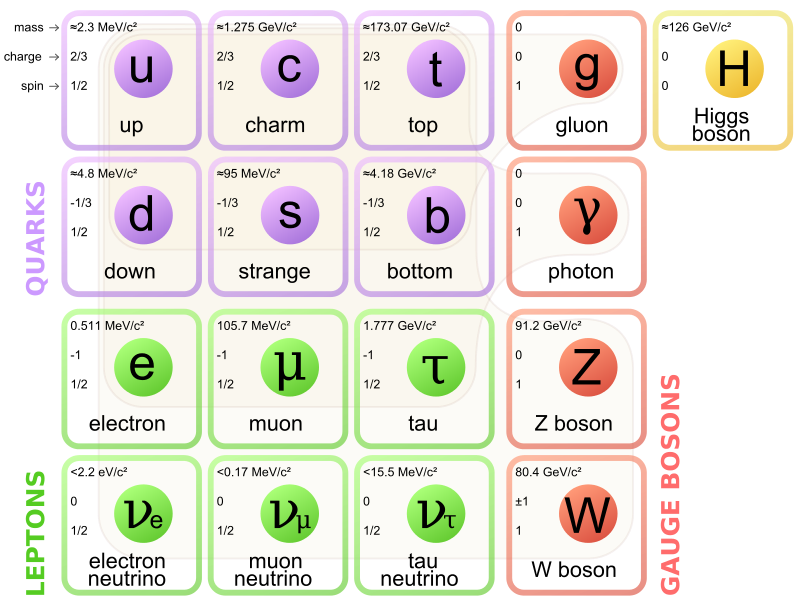
\includegraphics[width=0.7\textwidth]{figures/CLIC/StandardModel.png}
  \caption{The building blocks of matter according to the Standard
    Model~\cite{wikipediaParticles}.}
  \label{fig:standardmodel}
\end{figure}

Today, the Standard Model is the best theory describing the subatomic
world. However, it does not answer questions like the nature of dark
matter. This theory also predicts the existence of the Higgs boson
which gives the mass to all particles. It was experimentally observed
in 2012 by the ATLAS~\cite{Aad20121} and CMS~\cite{Chatrchyan201230}
experiments at CERN.

The weak and the electromagnetic forces are closely related to each
other and can be unified as the \textit{electroweak} interaction and
the equations describing the unification predict the force-carrying
particles (the photon, the W and Z bosons). All force-carrying
particles are described as being massless which is true for the
photon, but the W and Z bosons have a mass about 100 times larger than
that of the proton. To solve this problem, the Brout-Englert-Higgs
mechanism was introduced which suggests that the Higgs boson gives the
mass to the W and Z boson by interaction with a Higgs field.

The Higgs boson can be produced in a particle collider by collisions
between highly energetic particles. Heavy particles, like the Higgs
boson, are occasionally produced and detected by a particle
detector. The most important parameters of a particle collider are its
center-of-mass energy, determining the types of particles that can be
studied or discovered, and its instantaneous luminosity, determining
the event rates. For a given process, the cross section is a measure
of quantum mechanical probability for interaction and it depends on
the fundamental physics. Therefore, the observed number of events for
a given process depends on the integrated luminosity over the
operation time of the collider and the cross section of the
process. The Standard Model predicts different mechanisms to produce
the Higgs boson and the cross section is very small. For example, in
LHC only 1 Higgs boson is produced per 10 billion collisions.

An electron-positron collider allows to perform precision measurements
by colliding beams made of elementary particles. With elementary
particles, the center-of-mass energy and the polarisation of the
colliding particles can be selected precisely. Unlike proton-proton
collisions at the LHC experiments, there is no underlying event from
proton remnants. The complicated environment of a hadron machine makes
the measurements of the fundamental properties of the Higgs boson very
hard. The added value of an electron-positron collider would be to
measure in great details the Higgs mass and its total decay width, its
spin-parity quantum numbers, its couplings to fermions and gauge
bosons and also its self couplings that allows for the reconstruction
of the scalar potential that is responsible of electroweak symmetry
breaking~\cite{Linssen:1425915}.


CLIC is foreseen to be built and operated in three stages with
center-of-mass energies of $380\,\gev$, $1.5\,\tev$ and $3\,\tev$ as
shown in \cref{fig:CLICstaging}~\cite{Felzmann:2157041}. The site
studies have shown that CLIC could be placed near CERN
underground. For each stage, to increase the center-of-mass energy,
more accelerating modules will be needed, making the accelerator
longer. The site length for $3\,\tev$ will be 50~km.

\begin{figure}[htbp]
  \centering
  \includegraphics[width=0.7\textwidth]{figures/CLIC/staging.pdf}
  \caption{The three implementation stages of CLIC near CERN with
    center-of-mass energies of $380\,\gev$, $1.5\,\tev$ and
    $3\,\tev$~\cite{Felzmann:2157041}.}
  \label{fig:CLICstaging}
\end{figure}

The different energy stages at CLIC allow for maximising the
luminosity performance and physics potential for high precision
measurements of Standard Model physics (e.g. Higgs, top) as well as
new physics potentially discovered at the $13\,\tev$ LHC.

The first energy stage allows for studying the Standard Model Higgs
physics and top-quark physics with the possibility to perform a t\={t}
threshold scan. This stage gives the possibility to perform
model-independent cross-section
measurements~\cite{Abramowicz:2016zbo}. The second energy stage
provides direct sensitivity to many physics beyond the SM (BSM)
models. With larger Higgs statistics, rare processes such as t\={t}H
and double Higgs production can be measured. Finally, the third energy
stage provides the best sensitivity to new physics, the double-Higgs
production and allows for improving the measurements of the Higgs
self-coupling and HHWW quartic
coupling. \cref{fig:HiggsProductionMechanisms} shows different
mechanisms to produce the Higgs boson at CLIC.

\begin{figure}[htbp]
  \centering
  \begin{tikzpicture}
    % \node[anchor=south west,inner sep=0] (image) at
    % (0,0){\includegraphics[page=43, trim=30mm 235mm 25mm 30mm, clip,
    %   width=\textwidth]{figures/CLIC/clicCDR.pdf}};

    \node[anchor=south west,inner sep=0] (image) at
    (0,0){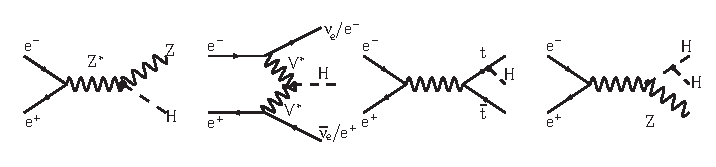
\includegraphics[width=\textwidth]{figures/CLIC/HiggsProductionMechanism.pdf}};
    
    \begin{scope}[x={(image.south east)},y={(image.north west)}]
      
      \node[below, color=black] at (0.14, 0.1)
      {e\textsuperscript{+}e\textsuperscript{-}$\rightarrow$ZH};

      \node[below, color=black] at (0.4, 0.1)
      {e\textsuperscript{+}e\textsuperscript{-}$\rightarrow$H$\nu_{e}\bar{\nu_{e}}$};

      \node[below, color=black] at (0.6, 0.1)
      {e\textsuperscript{+}e\textsuperscript{-}$\rightarrow$t\={t}H};

      \node[below, color=black] at (0.87, 0.1)
      {e\textsuperscript{+}e\textsuperscript{-}$\rightarrow$ZHH};
      
      % \draw[help lines,xstep=.1,ystep=.1] (0, 0) grid (1,1);
      % \foreach \x in {0,1,...,9} { \node [anchor=north] at (\x/10,0) {0.\x}; }
      % \foreach \y in {0,1,...,9} { \node [anchor=east] at (0,\y/10) {0.\y}; }
      
    \end{scope}
    
  \end{tikzpicture}
  \caption{Standard Model Higgs boson production mechanisms at
    CLIC~\cite{Linssen:1425915}.}
  \label{fig:HiggsProductionMechanisms}
\end{figure}

The cross sections to produce a Higgs with a mass of $M_H = 126\,\gev$
as a function of the center-of-mass energy $\sqrt{s}$ are given in
\cref{fig:corssSectionH125}. Below $\sqrt{s}$ of $\sim500\,\gev$, the
HZ mechanism is dominant. For higher energies, the
H$\nu_{e}\bar{\nu_{e}}$ mechanism dominates.

\begin{figure}[htbp]
  \centering
  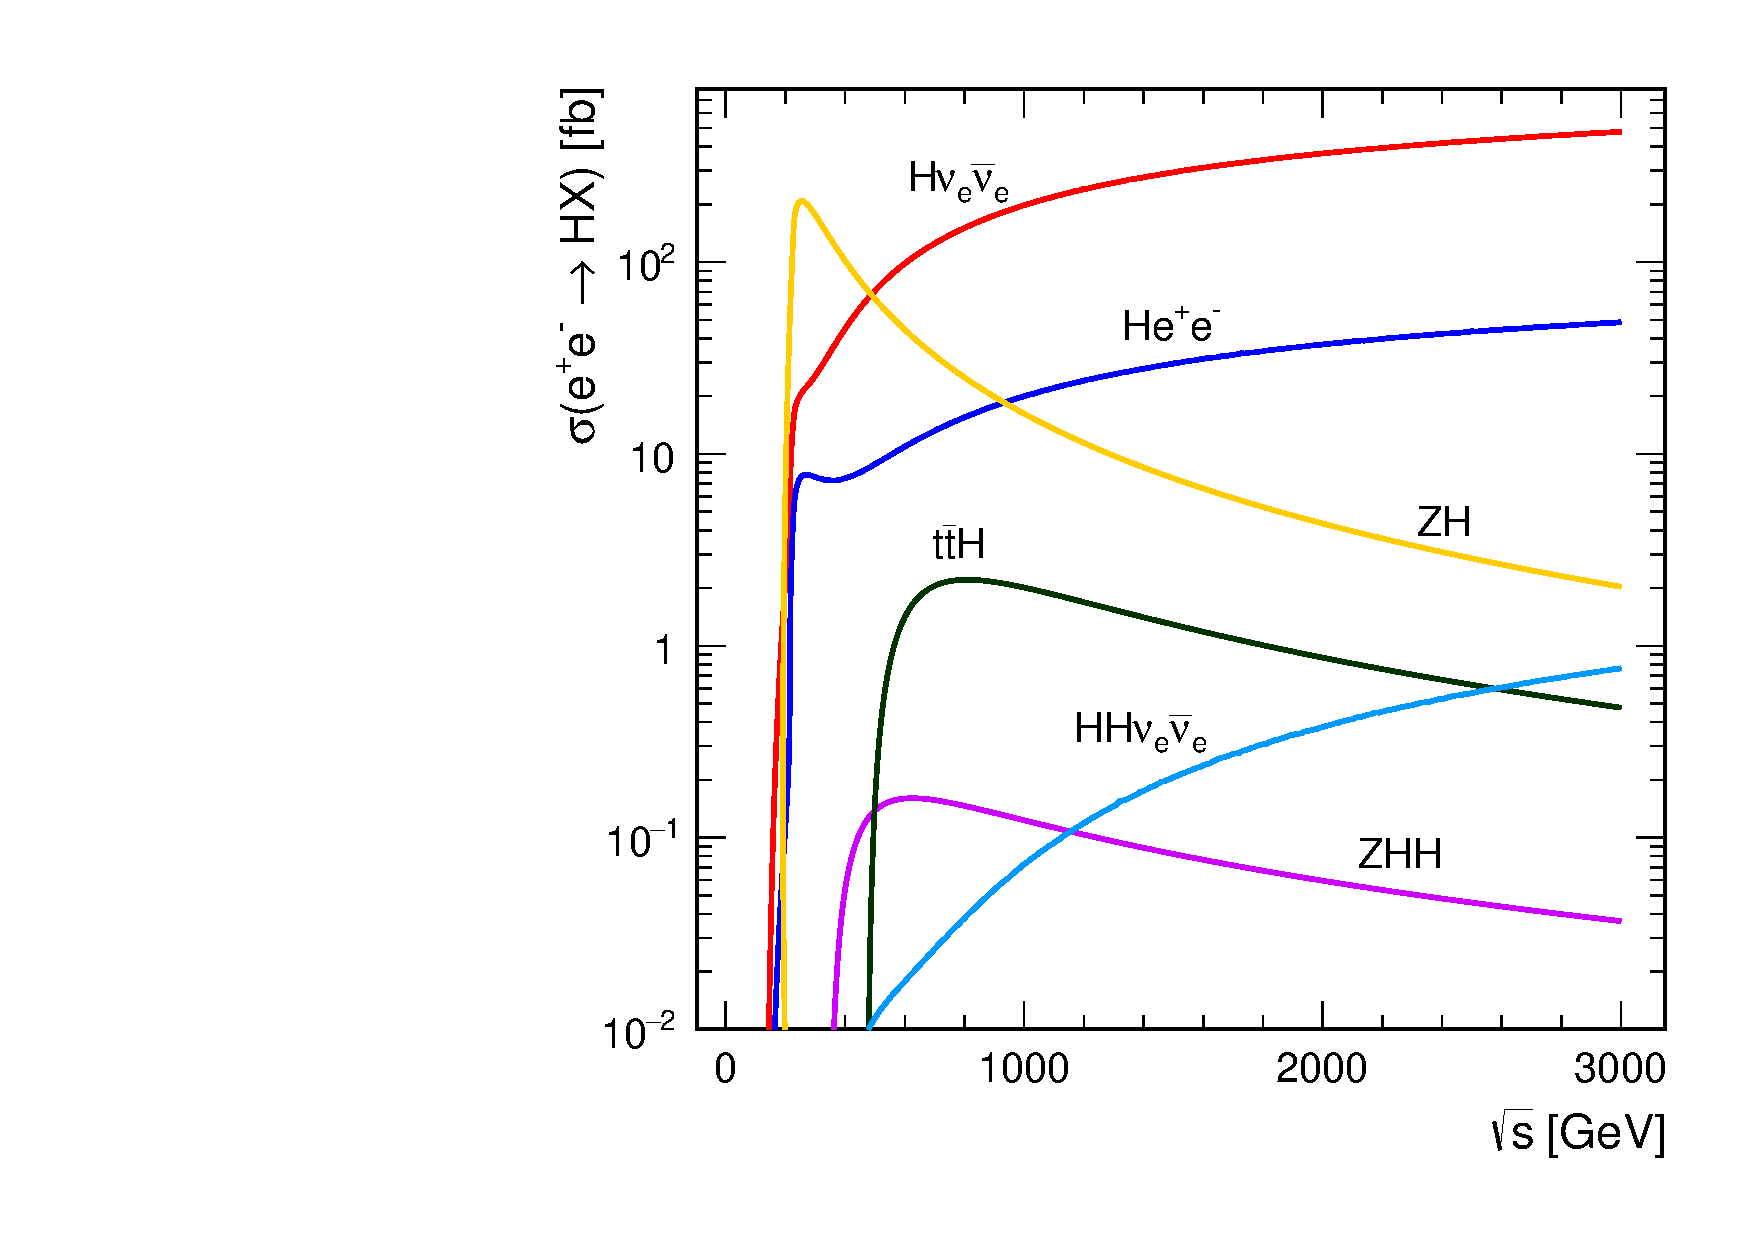
\includegraphics[width=0.5\textwidth]{figures/CLIC/xsec_vs_cme.pdf}
  \caption{Cross sections for the main Higgs production mechanisms for
    a $M_H~=~126\,\gev$ Higgs boson as a function of the e$^+$e$^-$
    center-of-mass energy in a lepton collider. These values
    correspond to unpolarised beams and the effect of beamstrahlung is
    not included~\cite{Felzmann:2157041}.}
  \label{fig:corssSectionH125}
\end{figure}

Final states with heavy quark flavours are important in many physics
channels, such as the Higgs and the top. The identification of the
heavy quarks is performed through the measurement of the displaced
vertices and the vertex detector has a crucial role in these
measurements as described in the following chapters.


\section{The CLIC accelerator}

The schematic layout of the CLIC accelerator complex at
$\sqrt{s}=3\,\tev$ is shown in \cref{fig:CLIC_accelerator}. The
electron and positron beams are accelerated on a linear trajectory and
collide in the central region (at the interaction point), where the
CLIC detector is placed. Each linac is fed by a drive-beam generation
complex.

\begin{figure}[htbp]
  \centering
  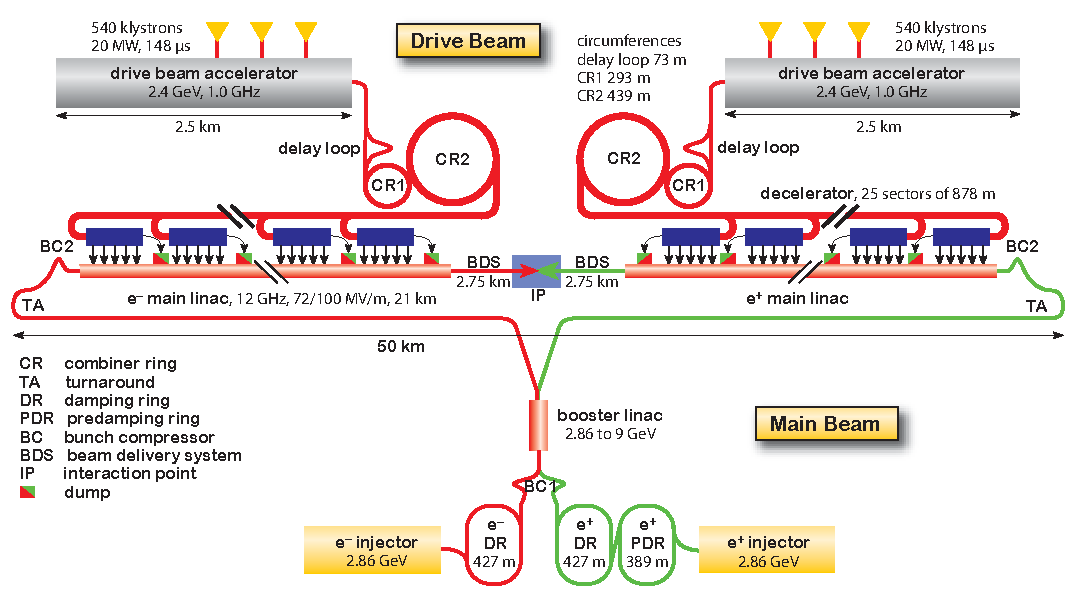
\includegraphics[width=\textwidth]{figures/CLIC/CLIC-layout2015pub.pdf}
  \caption{Schematic layout of the CLIC accelerator complex at
    $\sqrt{s}=3\,\tev$. Each linac is fed by a drive-beam generation
    complex~\cite{Felzmann:2157041}.}
  \label{fig:CLIC_accelerator}
\end{figure}

To limit the length of the accelerator, the accelerating field has to
be as high as possible. The accelerating gradient is chosen to be
100~MV/m. This leads to the use of copper cavities at room temperature
instead of superconducting cavities since the latter have an
intrinsically limited maximum field. The copper cavities are fed with
radio frequency (RF) power at a very high frequency of
$12\,\gigahertz$ to generate the high accelerating field. This leads
to a total RF peak power of 9.2~TW for both linacs. Since maintaining
such high power levels is not possible for very long, the duration of
the bunch train is limited to 156~ns with a repetition frequency of
50~Hz.


Traditionally, klystrons are used in accelerators to provide the RF
power to the main beam. However, for CLIC, klystrons are not directly
used to accelerate the main beam since a large number of them would be
needed and their efficiency would be too low at $12\,\gigahertz$. A
two-beam acceleration scheme is used to reach the nominal collision
energy. A drive beam is running in parallel to the main beam. The
drive beam has a low energy of $2.4\,\gev$ and a high current of
100~A. It is used to transfer the energy of the klystrons to the main
beam which has a lower current and higher energy. Power Extraction and
Transfer Structures (PETS) are special RF devices which extract the
power of the drive beam by decelerating the beam. The extracted energy
is then provided to the main beam. CLIC is divided into sectors with
an average length of 878~m and each section accelerates the main beam
by $\approx62\,\gev$.


\cref{tab:NominalMachineParams} summarises the nominal beam parameters
for the $3\,\tev$ CLIC and $13\,\tev$ LHC. An instantaneous luminosity
$\mathcal{L}$ of a few $10^{34}$~\inversecmsquaredsec insures a
sufficient amount of data collected in a reasonable amount of
time. The beam sizes at the interaction point of CLIC have to be
extremely small in order to achieve the desired luminosity. The RF
pulse duration limits the number of bunches and the bunch-crossing
separation. CLIC and LHC have similar luminosity despite the
differences in beam parameters.

\begin{table}[htbp]
  \centering
  \caption{Nominal beam parameters for CLIC at $\sqrt{s}=3\,\tev$ and
    LHC at $\sqrt{s}=13\,\tev$.}
  \label{tab:NominalMachineParams}
  \begin{tabular}{l c c}
    \toprule
    & CLIC at $\sqrt{s}=3\,\tev$ & LHC at $\sqrt{s}=13\,\tev$\\
    \midrule
    Colliding particles & electron-positron & proton-proton \\
    Instantaneous luminosity $\mathcal{L}$ & $6\times10^{34}$ \inversecmsquaredsec & $1\times10^{34}$ \inversecmsquaredsec \\
    Bunch-crossing separation & 0.5~ns & 25~ns \\
    Bunches per train & 312 & Not applicable \\
    Train duration & 156~ns & Not applicable \\
    Train repetition & 50~Hz & Not applicable \\
    IP size in x / y / z directions & 45~nm / 1~nm / $44\,\micron$ & $15\,\micron$ / $15\,\micron$ / 50~cm \\
    \bottomrule
  \end{tabular}
\end{table}

\subsection{Beam-induced backgrounds}
\label{sec:beamInducedBackgrounds}

The small beam sizes at CLIC cause strong electromagnetic radiation
(Beamstrahlung) from the electron and positron bunches in the field of
the opposite beam. The generation of Beamstrahlung photons leads to a
reduction of the available centre-of-mass energy $\sqrt{s}$ of the
e\textsuperscript{+}e\textsuperscript{-} collisions. The interactions
of Beamstrahlung photons produce lepton pairs and hadrons at low polar
angles which are mostly contained in the
beam-pipe~\cite{Dannheim:1443516}. In the inner detector layers,
incoherently produced electron-positron pairs ($\sim60$ particles per
bunch crossing) and $\gamma\gamma\rightarrow$hadrons events ($\sim54$
particles per bunch crossing) are the dominant backgrounds.

The electron-positron pairs produced at low polar angles have very
small transverse momentum. The occupancies in the innermost layers of
the detector can be reduced to an acceptable level by optimising the
inner and forward detector regions. The beam-pipe walls have to be
placed outside of the high-rate region. The inner detectors have to be
shielded from the backscattered particles which originate from the
forward region.

The $\gamma\gamma\rightarrow$hadrons interactions produce particles
with a higher transverse momentum spectrum and a more central
polar-angle distribution. This results in large rates of background
particles reaching the outer detector layers. In each train, at most
one interesting physics event is expected along with $\sim1000$
hadronic background events.

Hit time stamping on the level of 1 to 10~ns in all sub-detectors is
needed in order to separate the physics from the background events.

The exposure to radiation of the main detector elements is expected to
be small compared to high-energy hadron-colliders.

\section{The CLIC detector}
\label{sec:CLICdetector}

To cover the CLIC physics potential, a detector concept is under
development. The physics goals set challenging requirements on the
design of the detector. Simulation tools are crucial for the design,
development as well as the optimisation of the detector model.

The experimental conditions due to the beam-induced background (see
\cref{sec:beamInducedBackgrounds}), set the most demanding
requirements at the highest collision energy. Therefore, the detector
model is mainly optimised for the $3\,\tev$ CLIC.

\cref{fig:CLIC_detector_concept} shows the CLIC detector model as
implemented in simulations. The overall length and height of the
detector are 11.4~m and 12.9~m respectively. It is composed of several
sub detectors. The vertex detector is the closest to the IP and
consists of pixelated silicon detectors. It is followed by the main
tracker which is also a silicon-based detector. After the tracking
systems, fine grained calorimeters are used: the silicon-tungsten
electromagnetic calorimeter (ECAL) and the steel hadronic calorimeter
(HCAL). The superconducting coil surrounds the calorimeters to provide
a magnetic field of 4~T to deflect the trajectory of charged
particles. The tracking detectors use the radius of curvature to
measure the momentum of charged particles. In the very forward region,
the luminosity calorimeter (LumiCal) is used to reconstruct precisely
the energy and angle of electrons and positrons obtained from Bhabha
events and employed for the luminosity
measurements~\cite{Abramowicz:2010bg}. The beam calorimeter (BeamCal)
is used for electron tagging by the identification of high energy
electrons~\cite{Abramowicz:2004me}. Finally the iron yoke surrounds
the whole detector and is instrumented for the identification of
muons.


\begin{figure}[htbp]
  \centering
  \begin{tikzpicture}
    \node[anchor=south west,inner sep=0] (image) at
    (0,0){\includegraphics[width=0.62\textwidth]{figures/CLIC/CLICdp_Top_view_HD_temp.pdf}};
    \begin{scope}[x={(image.south east)},y={(image.north west)}]
      %% \draw[help lines,xstep=.1,ystep=.1] (0, 0) grid (1,1);
      %% \foreach \x in {0,1,...,9} { \node [anchor=north] at (\x/10,0) {0.\x}; }
      %% \foreach \y in {0,1,...,9} { \node [anchor=east] at (0,\y/10)
      %% {0.\y}; }
      \node[draw, text width=2cm] at (-0.2, 0.9) {Ultra low-mass vertex detector};
      \draw[->,line width=1pt, color=black](-0.02, 0.9) -- (0.5, 0.5);

      \node[draw, text width=2cm] at (-0.2, 0.7) {Main tracker, silicon based};
      \draw[->,line width=1pt, color=black](-0.02, 0.7) -- (0.35, 0.55);

      \node[draw, text width=2cm] at (-0.2, 0.5) {Forward region with LumiCal \& BeamCal};
      \draw[->,line width=1pt, color=black](-0.02, 0.45) -- (0.25, 0.49);

      \node[draw, text width=2cm] at (-0.2, 0.2) {Fine grained
        calorimetry optimised for Particle Flow Analysis (PFA)};
      \draw[->,line width=1pt, color=black](-0.02, 0.2) -- (0.3, 0.3);

      \node[draw, text width=2cm] at (1.15, 0.15) {Return yoke (Fe) with detectors for muon ID};
      \draw[->,line width=1pt, color=black](1, 0.1) -- (0.8, 0.1);

      \node[draw, text width=2cm] at (1.15, 0.79) {Solenoid magnet: B=4~T};
      \draw[->,line width=1pt, color=black](1, 0.79) -- (0.8, 0.79);
      

      \node[color=black] at (0.5, 0.05) {11.4~m};
      \draw[<->,line width=1pt, color=black](0.03, 0.02) -- (0.97,
      0.02);

      \node[color=black] at (1.1, 0.5) {12.9~m};
      \draw[<->,line width=1pt, color=black](0.99, 0.01) -- (0.99, 0.99);
      
      % \draw[help lines,xstep=.1,ystep=.1] (0, 0) grid (1,1);
      % \foreach \x in {0,1,...,9} { \node [anchor=north] at (\x/10,0) {0.\x}; }
      % \foreach \y in {0,1,...,9} { \node [anchor=east] at (0,\y/10) {0.\y}; }
      
    \end{scope}
  \end{tikzpicture} 
  \caption{Schematic layout of the CLIC detector
    concept~\cite{CLICdetUnpublishedNote}.}
  \label{fig:CLIC_detector_concept}
\end{figure}

\subsection{Requirements for the vertex-detector}
\label{sec:VXD_requirements}

The main goal of the CLIC vertex detector is the efficient tagging of
heavy quarks through the precise measurement of the displaced
vertices. To achieve this goal, Monte Carlo simulations have shown
that a high-momentum term in the transverse impact-parameter
resolution of $a\approx5\,\micron$ and a multiple-scattering term of
$b\approx15\,\micron$ are needed using the canonical
parametrisation~\cite{Linssen:1425915}:

\begin{equation}
 \sigma(d_0)=\sqrt{a^2+b^2 \cdot\gev^2/(p^2 \text{sin}^3\theta)} \; ,
  \label{eq:canonicalParam}
\end{equation}

where $p$ is the momentum of the particle and $\theta$ is the polar
angle with respect to the beam axis.

To meet these requirements, a multi-layer barrel and endcap pixel
detector with an inner radius of $\approx$30~mm with a geometrical
coverage extending down to low polar angles
($\theta_{min}\approx8^{\circ}$) is needed. For the beam-pipe and for
each of the detection layers a material budget of $\approx0.2\%$ of a
radiation length (X\textsubscript{0}) is considered. Sensors with a
single-point resolution of $\approx3\,\micron$ operating in a magnetic
field of 4~T are required.

In the innermost layers, an occupancy of $\approx3\%$ due to the
beam-induced backgrounds is expected~\cite{Dannheim:1443516}. To
separate these backgrounds from physics events, a time slicing of the
hits with an accuracy of $\approx10$~ns is required. To achieve this
precise time stamping, hybrid detectors (where sensors and electronics
are separately manufactured and later combined) are preferred since
they provide more advanced timing measurement technologies.

In comparison to the current pixel detectors in the LHC experiments,
the expected radiation level in the region of the CLIC vertex detector
is moderate. For the inner-detector layers a total $1\,\mev$
neutron-equivalent fluence of less than
$10^{11}$~neq/cm\textsuperscript{2}/year and a total ionising dose of
less than 1~kGy are expected~\cite{Dannheim:1443516}.

The aim of the vertex detector R\&D is to achieve the required
single-point resolution with pixels of size
$\approx25\,\micron\times25\,\micron$ with $50\,\micron$ thick sensors
coupled to $50\,\micron$ thick readout ASICs with pulse-height
measurement capability. The constraint on the material budget implies
no active cooling elements can be placed inside the vertex
detector. To limit the maximum power dissipation of the readout
electronics to $\approx50~\text{mW/cm}^2$, forced air-flow cooling and
power pulsing (i.e. turning off most components on the readout chips
during the 20~ms gaps between bunch trains) are foreseen.

\section{Flavour-tagging performance at CLIC}
\label{sec:flavourTagging}

The precision physics measurements require excellent flavour-tagging
performance of the CLIC vertex detector. Different vertex detector
geometries have been studied for
CLIC~\cite{AlipourTehrani:1742993,Tehrani:2015tla}. This section
presents the impact of the geometry on the flavour-tagging performance
in simulations. This study has been published
in~\cite{Tehrani:2015tla}.

A first geometry designed for the CLIC vertex detector is shown in
\cref{fig:disksGeom}. It contains 5 layers in the barrel and 4 disks
in the endcap region. Since forced airflow cooling is foreseen for
CLIC as illustrated in \cref{fig:cooling}, a spiral arrangement for
the modules in the endcap regions has been implemented instead of
disks, allowing the air to flow through the vertex detector.

\begin{figure}[htbp]
  \centering
  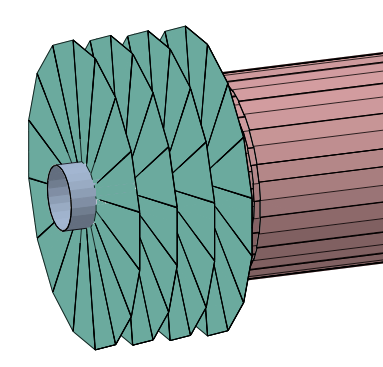
\includegraphics[width=0.4\textwidth]{figures/CLIC/cdr.png}
  \caption{The schematic view of the disks geometry with 5
    single-sided layers in the barrel region and 4 single-sided disks
    in the endcap region.}
  \label{fig:disksGeom}
\end{figure}

The physics performance of the geometries described in
Table~\ref{tab:geometries} and illustrated in
Figure~\ref{fig:geometries} have been studied in simulations.


The multi-variate LCFIPlus flavour-tagging
package~\cite{website:LCFIPlus} is used to assign each jet category
with a beauty (b) and charm (c) probability. The fake rates of
separating the charm and beauty jets from each other and from light
flavour (LF) jets have been investigated.

The detector models in simulation consider the single-point resolution
of the sensors ($\sim3\,\micron$) and include layer thicknesses based
on constraints from an engineering model of the mechanical support and
the air cooling system~\cite{AlipourTehrani:1742993}.


\begin{table}[htbp]
  \caption{Vertex detector geometries implemented in simulations.}
  \begin{center}
    \begin{tabular}{ l c c c }
      \hline
      Geometry & Barrel layers & Endcap layers & Material budget \\ \hline \hline
      \emph{spirals} (Figure~\ref{fig:SpiralsGeometry}) & 5 single-sided & 4 single-sided & $0.1\%X_{0}$ per single-sided layer  \\ %\hline 
      \emph{double\_spirals} (Figure~\ref{fig:doubleLayer}) & 3 double-sided & 3 double-sided & $0.2\%X_{0}$ per double-sided layer  \\ %\hline
      \emph{double\_spirals\_v2} & 3 double-sided & 3 double-sided & $0.4\%X_{0}$ per double-sided layer  \\ \hline  
    \end{tabular}
  \end{center}
  \label{tab:geometries}
\end{table}


\begin{figure}[htbp]
  \begin{subfigure}[b]{0.33\textwidth}
    \centering
    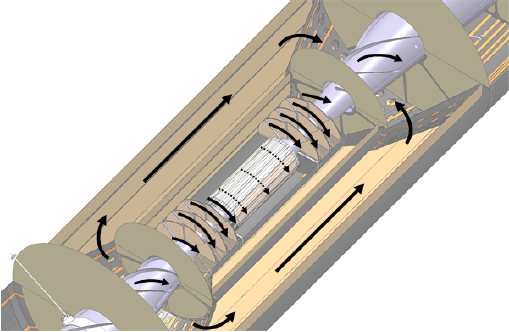
\includegraphics[width=\textwidth]{figures/CLIC/Cooling.png}  
    \caption{}
    \label{fig:cooling}
  \end{subfigure}~
  \begin{subfigure}[b]{0.33\textwidth}
    \centering
    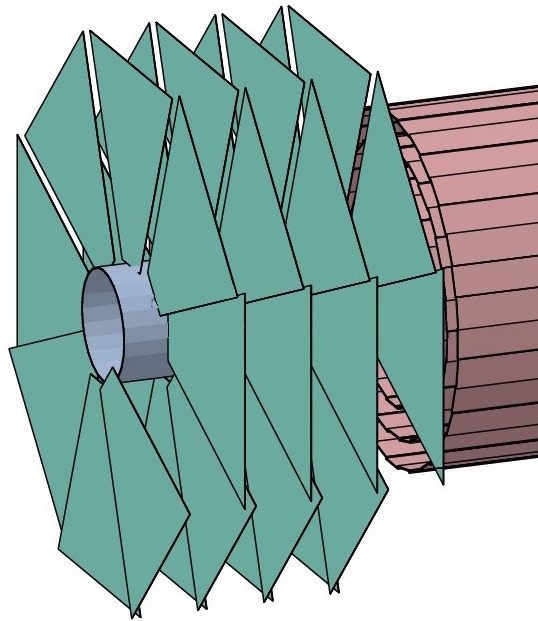
\includegraphics[width=0.65\textwidth]{figures/CLIC/single_spiral.jpg}
    \caption{}
    \label{fig:SpiralsGeometry}
  \end{subfigure}~
  \begin{subfigure}[b]{0.25\textwidth}
    \centering
    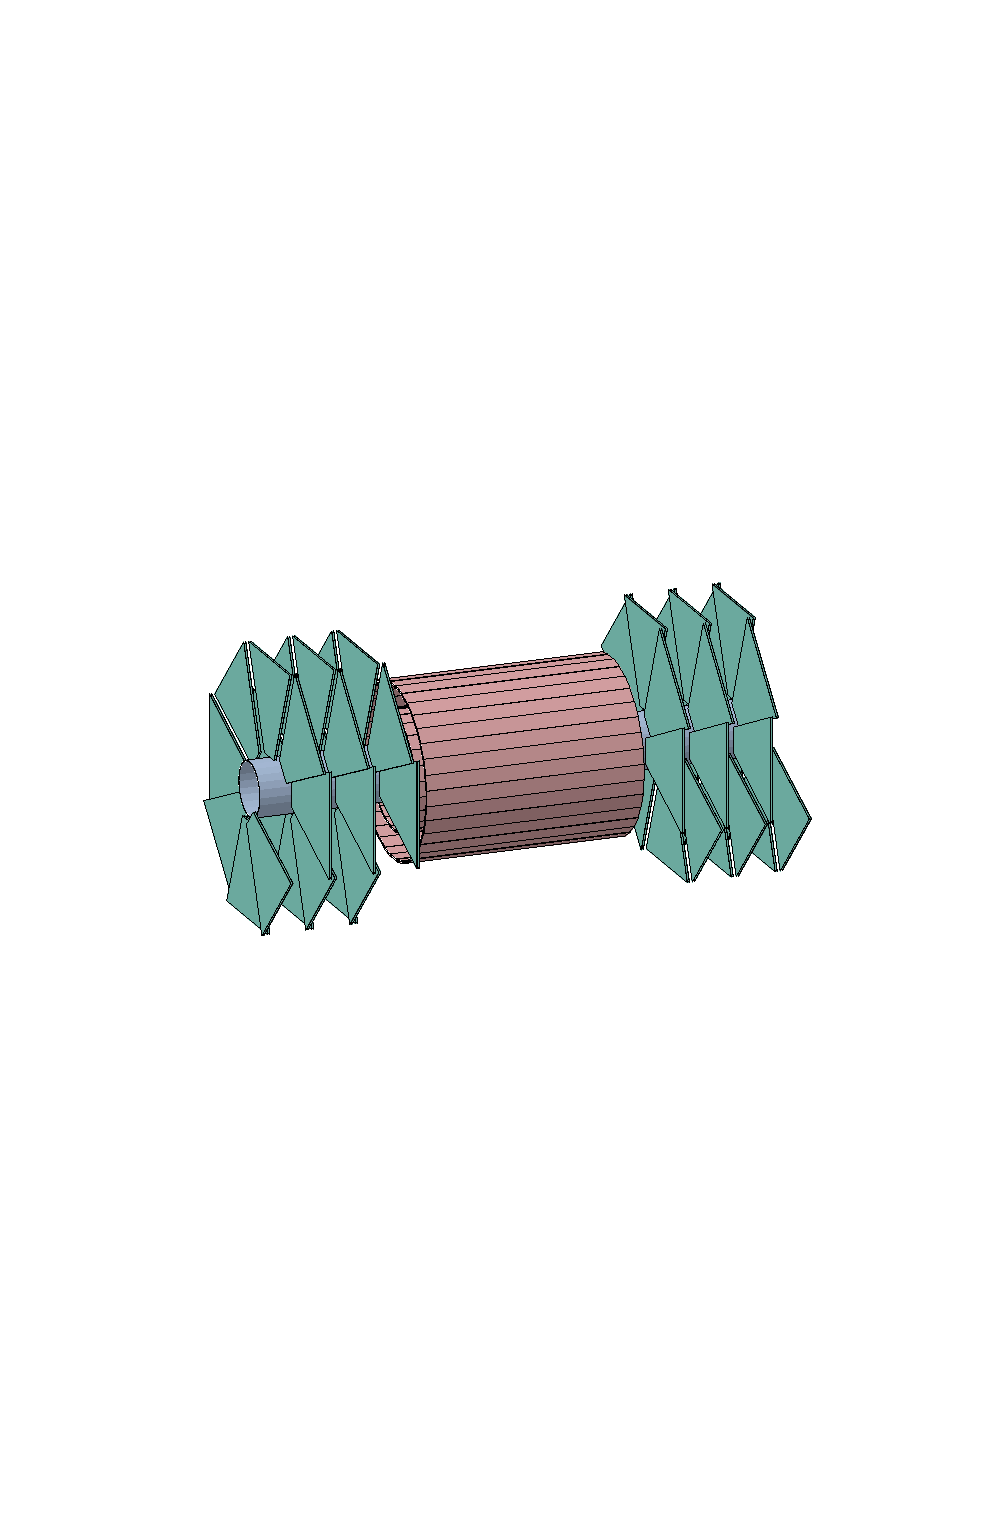
\includegraphics[trim = 32mm 98mm 85mm 106mm, clip, width=0.65\textwidth]{figures/CLIC/double_spiral.pdf} \\
    
\includegraphics[width=1.5\textwidth]{figures/CLIC/double_layer_module.png} 
    \caption{}
    \label{fig:doubleLayer}
  \end{subfigure}
  \caption{(a)~Sketch showing the airflow cooling strategy within the
    vertex detector~\cite{DuarteRamos:1572989}. (b)~Schematic view of
    the vertex detector for the \emph{spirals} geometry. (c)~Schematic
    view of the vertex detector for the
    \emph{double\_spirals(\_v2)}. In the \textsc{GEANT4}
    simulations~\cite{Agostinelli:2002hh}, a double-sided layer is
    implemented as two silicon sensors on top of each other with an
    overall thickness of
    \SI{2}{\milli\meter}. From~\cite{Tehrani:2015tla}.}
  \label{fig:geometries}
\end{figure}

The performance of the flavour tagging depends on the jet energy and
polar angle: dijet events with different center-of-mass energies,
$\sqrt{s}$, having polar angles of
$10^{\circ} \leq \theta \leq 90^{\circ}$ with a uniform distribution
in azimuthal $\phi$ angles are considered. Initial state radiation
(ISR) and beamstrahlung (BS) were switched off during the event
generation and hence the final-state quarks are in a back-to-back
configuration. For each jet flavour, energy and angle, 80000 events
are used for the following processes: e$^+$e$^-$ $\rightarrow$ b\={b},
c\={c}, u\={u}, d\={d}, s\={s}. The boosted decision tree (BDT)
classifiers are trained using 50\% of the generated events and the
other 50\% are used for testing the performance of the flavour
tagging.

\cref{fig:DisksPerformance} shows the dependence of the
flavour-tagging performance on the jet polar angle in the
\textit{disks} geometry for jets in dijet events at
$\sqrt{s}=200\,\gev$. \cref {fig:DisksPerformance_btag} shows the fake
rate of recognising beauty jets as charm jets versus the
beauty-tagging efficiency. For dijet events at $\theta=40^{\circ}$,
for a b-tagging efficiency of $80\%$, the probability to misidentify
charm quarks as beauty quarks is
$\sim5\%$. \cref{fig:DisksPerformance_ctag} shows the fake rate of
recognising charm jets as beauty jets versus the charm-tagging
efficiency. As expected, the b-tagging performance is better than the
c-tagging performance. However, CLIC allows for a higher charm tagging
performance compared to the LHC experiments.

\begin{figure}
  \begin{subfigure}[b]{0.49\textwidth}
    \centering
    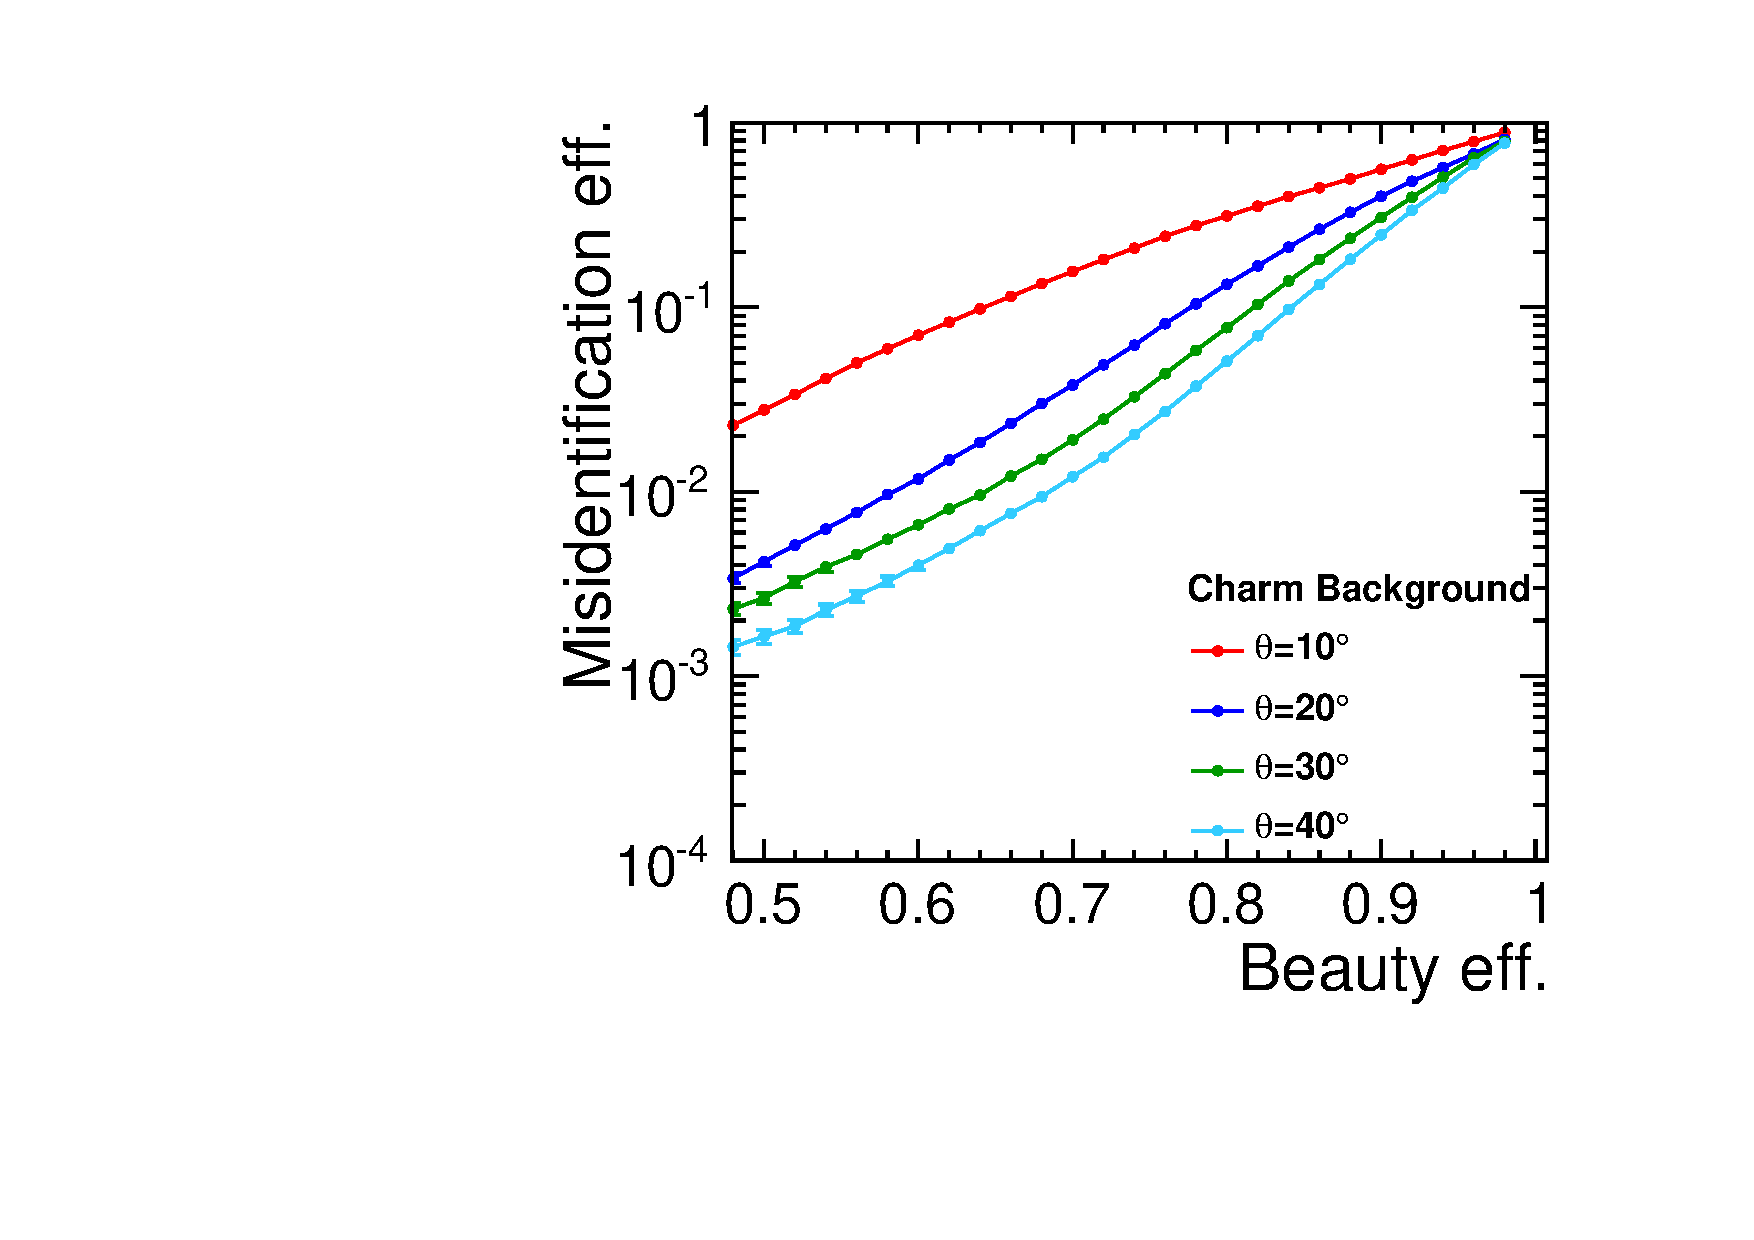
\includegraphics[width=\textwidth]{figures/CLIC/allAngles_CLIC_SiD_CDR_Beauty_Charm_200.pdf}
    \caption{}\label{fig:DisksPerformance_btag}
  \end{subfigure}\hfill
  \begin{subfigure}[b]{0.49\textwidth}
    \centering
    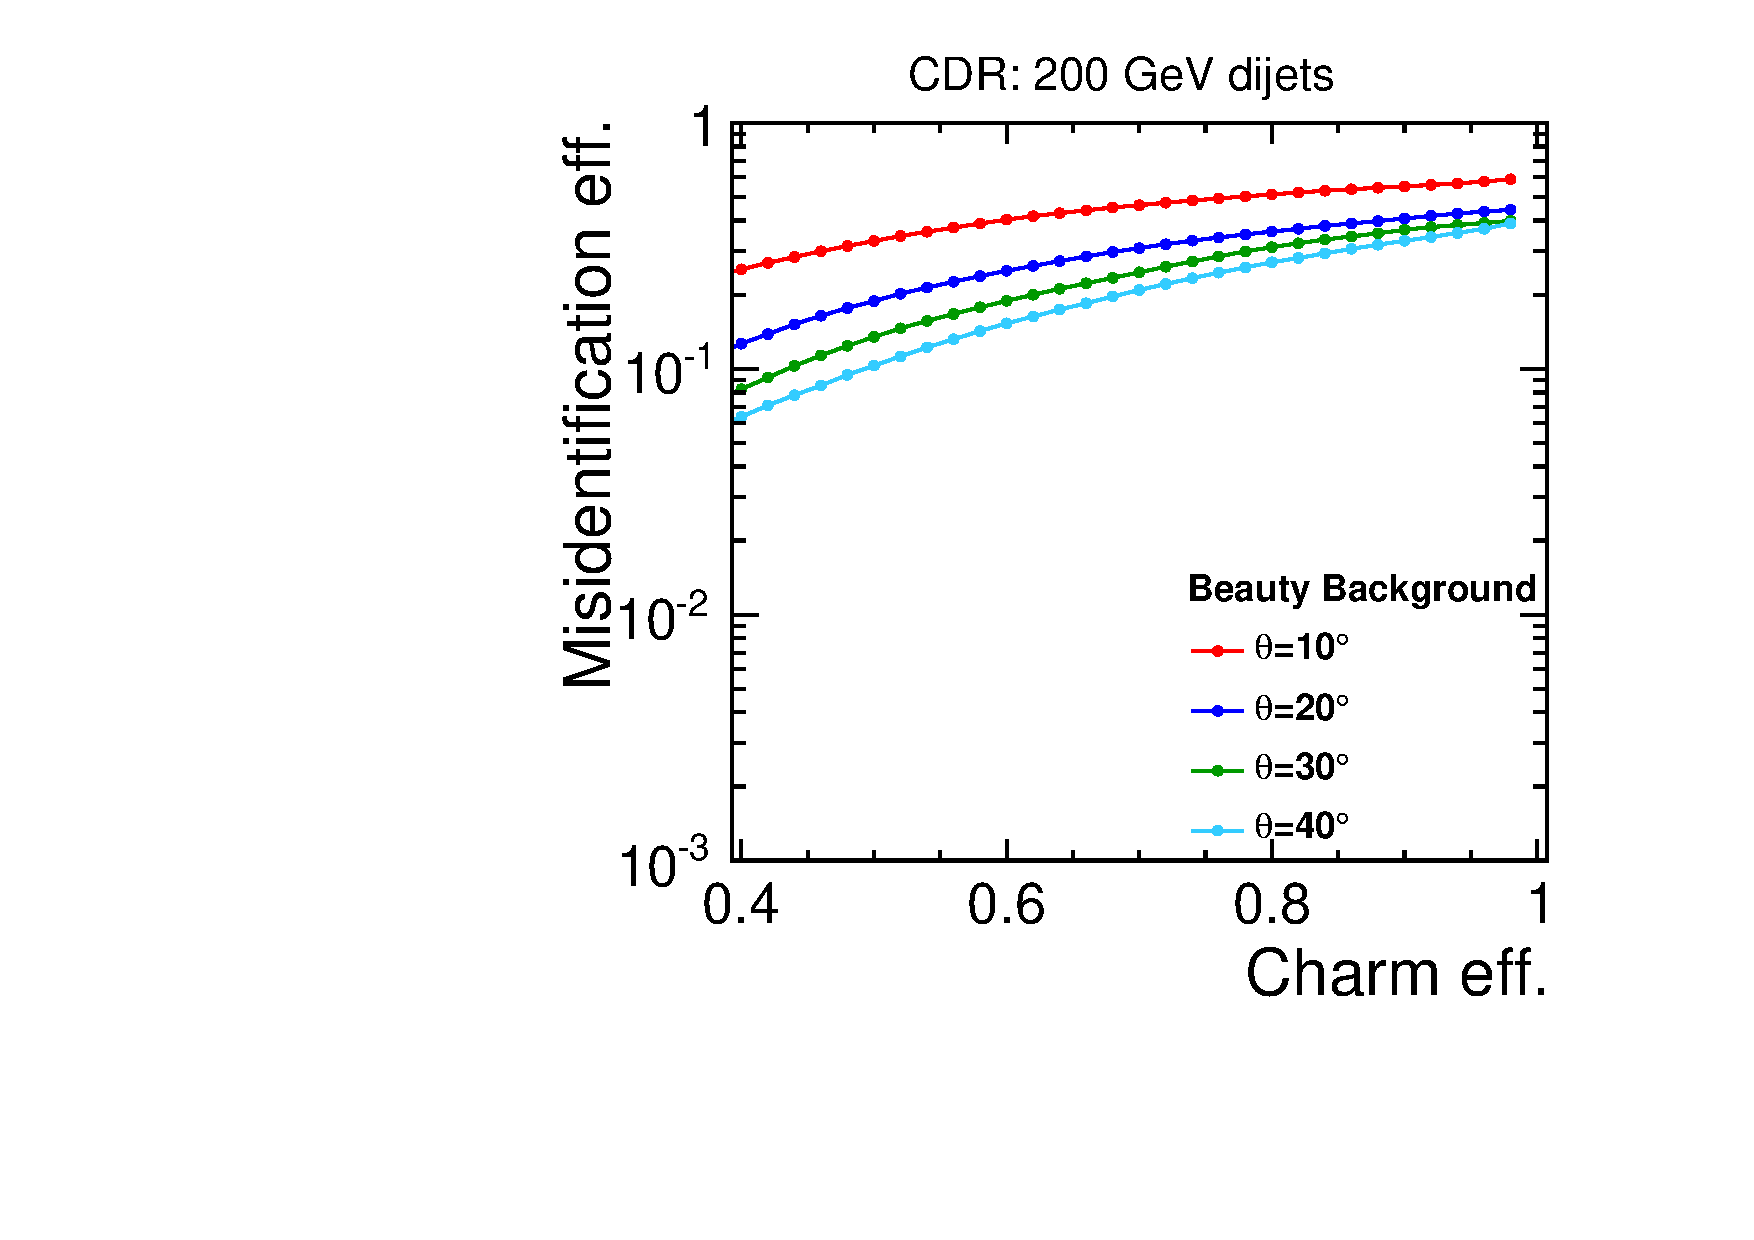
\includegraphics[width=\textwidth]{figures/CLIC/allAngles_CLIC_SiD_CDR_Charm_Beauty_200.pdf}
    \caption{}\label{fig:DisksPerformance_ctag}
  \end{subfigure} 
  \caption{(a) b-tag and (b) c-tag efficiency for jets in dijet events
    at $\sqrt{s}=200\,\gev$ with different polar angles for the
    \textit{disks} geometry~\cite{AlipourTehrani:1742993}.}
  \label{fig:DisksPerformance}
\end{figure}

The flavour-tagging performance for the different vertex detector
geometries as shown in \cref{fig:geometries} is summarised in
\cref{fig:performance} where the fake rate of recognising charm and
light flavour jets as beauty jets is plotted versus the b-tag
efficiency.

The \emph{spirals} and \emph{disks} have a similar flavour-tagging
performance except for jets at $\theta=40^{\circ}$ (see
Figure~\ref{fig:spiral_disks}), which corresponds to the transition
between the vertex endcaps and the barrel region, where the
beauty-tagging performance is up to $20\%$ worse using the
\emph{spirals} geometry (compared to disks). With the spiral
configuration, the number of sensitive layers becomes dependent on the
azimuthal angle $\phi$ and fewer layers can be hit in certain ranges
of $\phi$. The performance degradation caused by this $\phi$
dependence can be mitigated by increased $\phi$ overlap in future
geometry implementations.

The performance of the \emph{spirals} and the \emph{double\_spirals}
is very similar as shown in Figure~\ref{fig:spiral_doubleSpirals}.
The \emph{double\_spirals\_v2} geometry is a more realistic version of
the \emph{double\_spirals} geometry, taking into account the material
used for the mechanical support of the sensors and also for the
cables. As shown in Figure~\ref{fig:doubleSpirals_doubleSpirals}, the
misidentification probability increases by $\sim$35\% due to the
increased material.


\begin{figure}[htbp]
  \begin{subfigure}[b]{0.33\textwidth}
    \centering
    \begin{tikzpicture}
      \node[anchor=south west, inner sep=0] (image) at (0,0){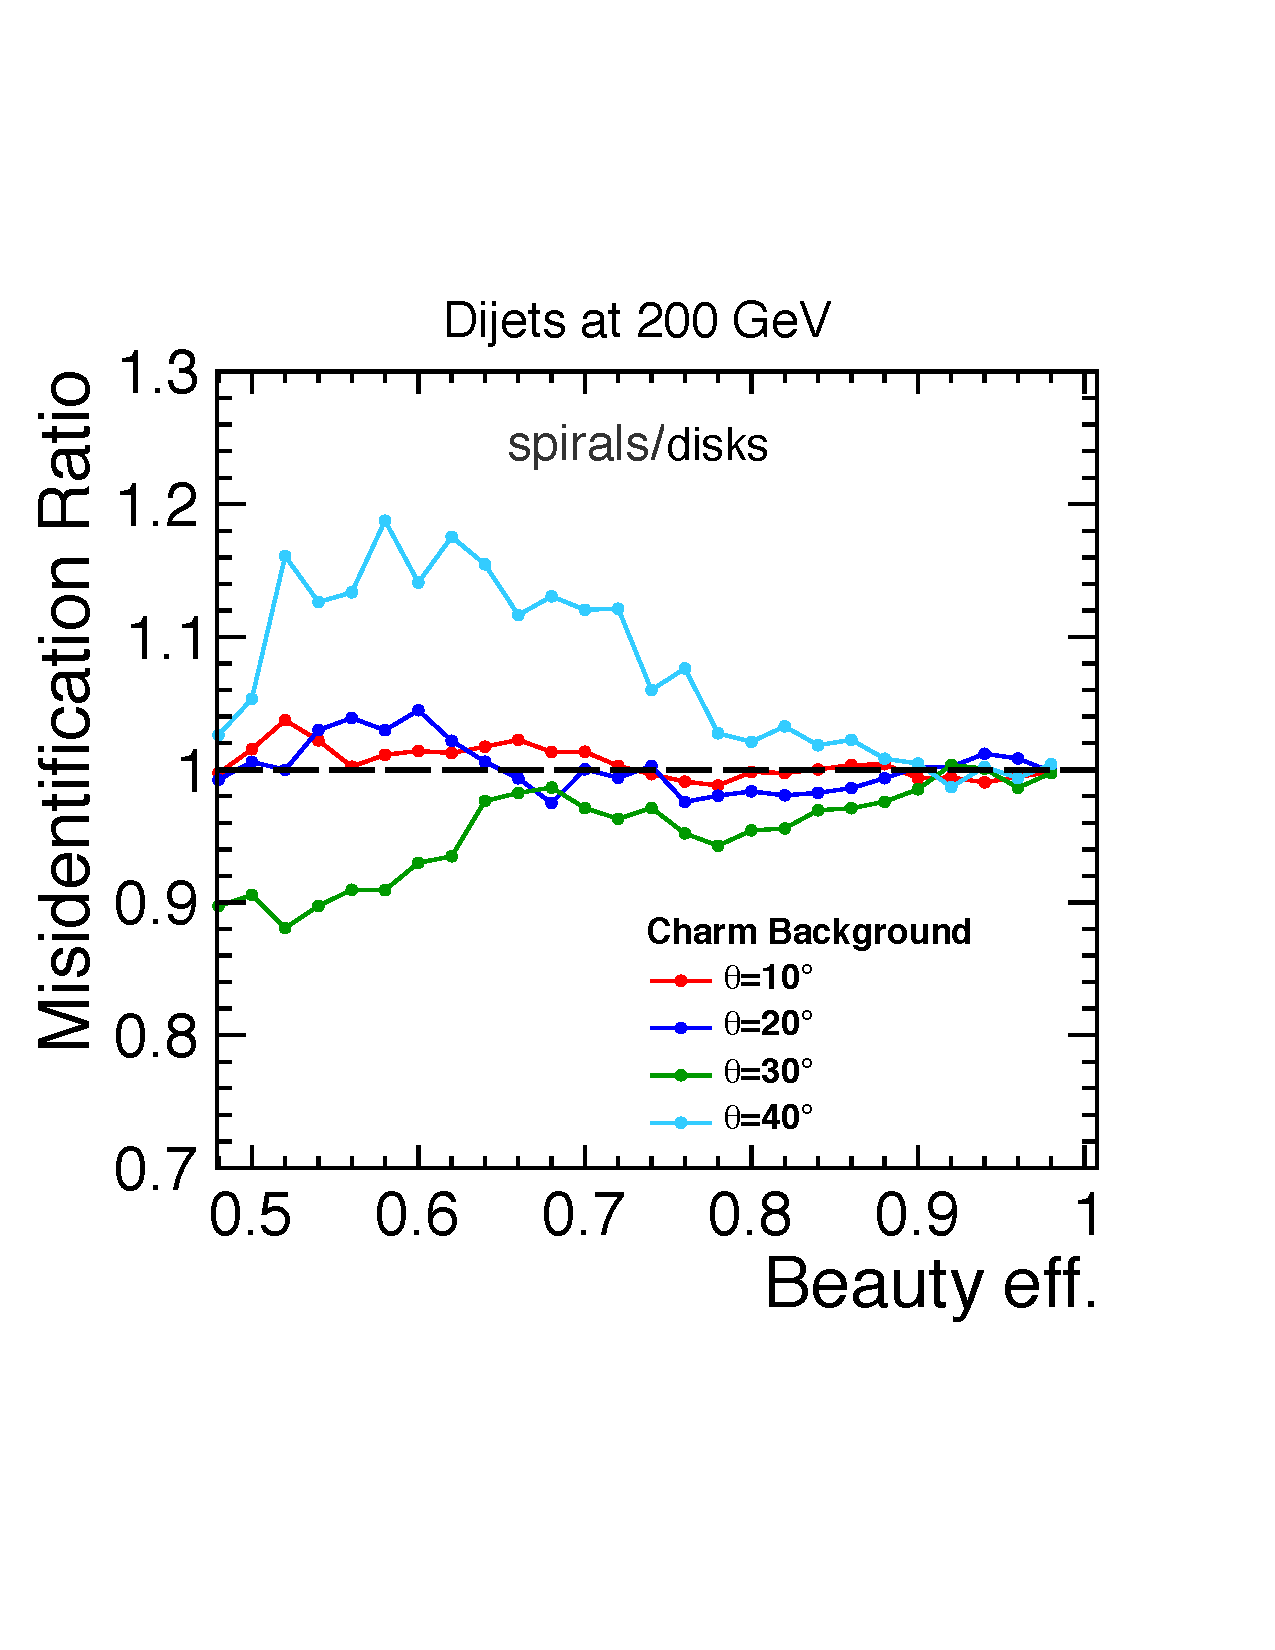
\includegraphics[trim = 5mm 50mm 20mm 20mm, clip, width=\textwidth]{figures/CLIC/200GeV_Ratio_allAngles_spirals_CDR_B_C.pdf}};
      \draw  (1.8, 1.5) node {\textbf{CLICdp}};
    \end{tikzpicture}
    \caption{}
    \label{fig:spiral_disks}
  \end{subfigure}~
  \begin{subfigure}[b]{0.33\textwidth}
    \centering
    \begin{tikzpicture}
      \node[anchor=south west, inner sep=0] (image) at (0,0){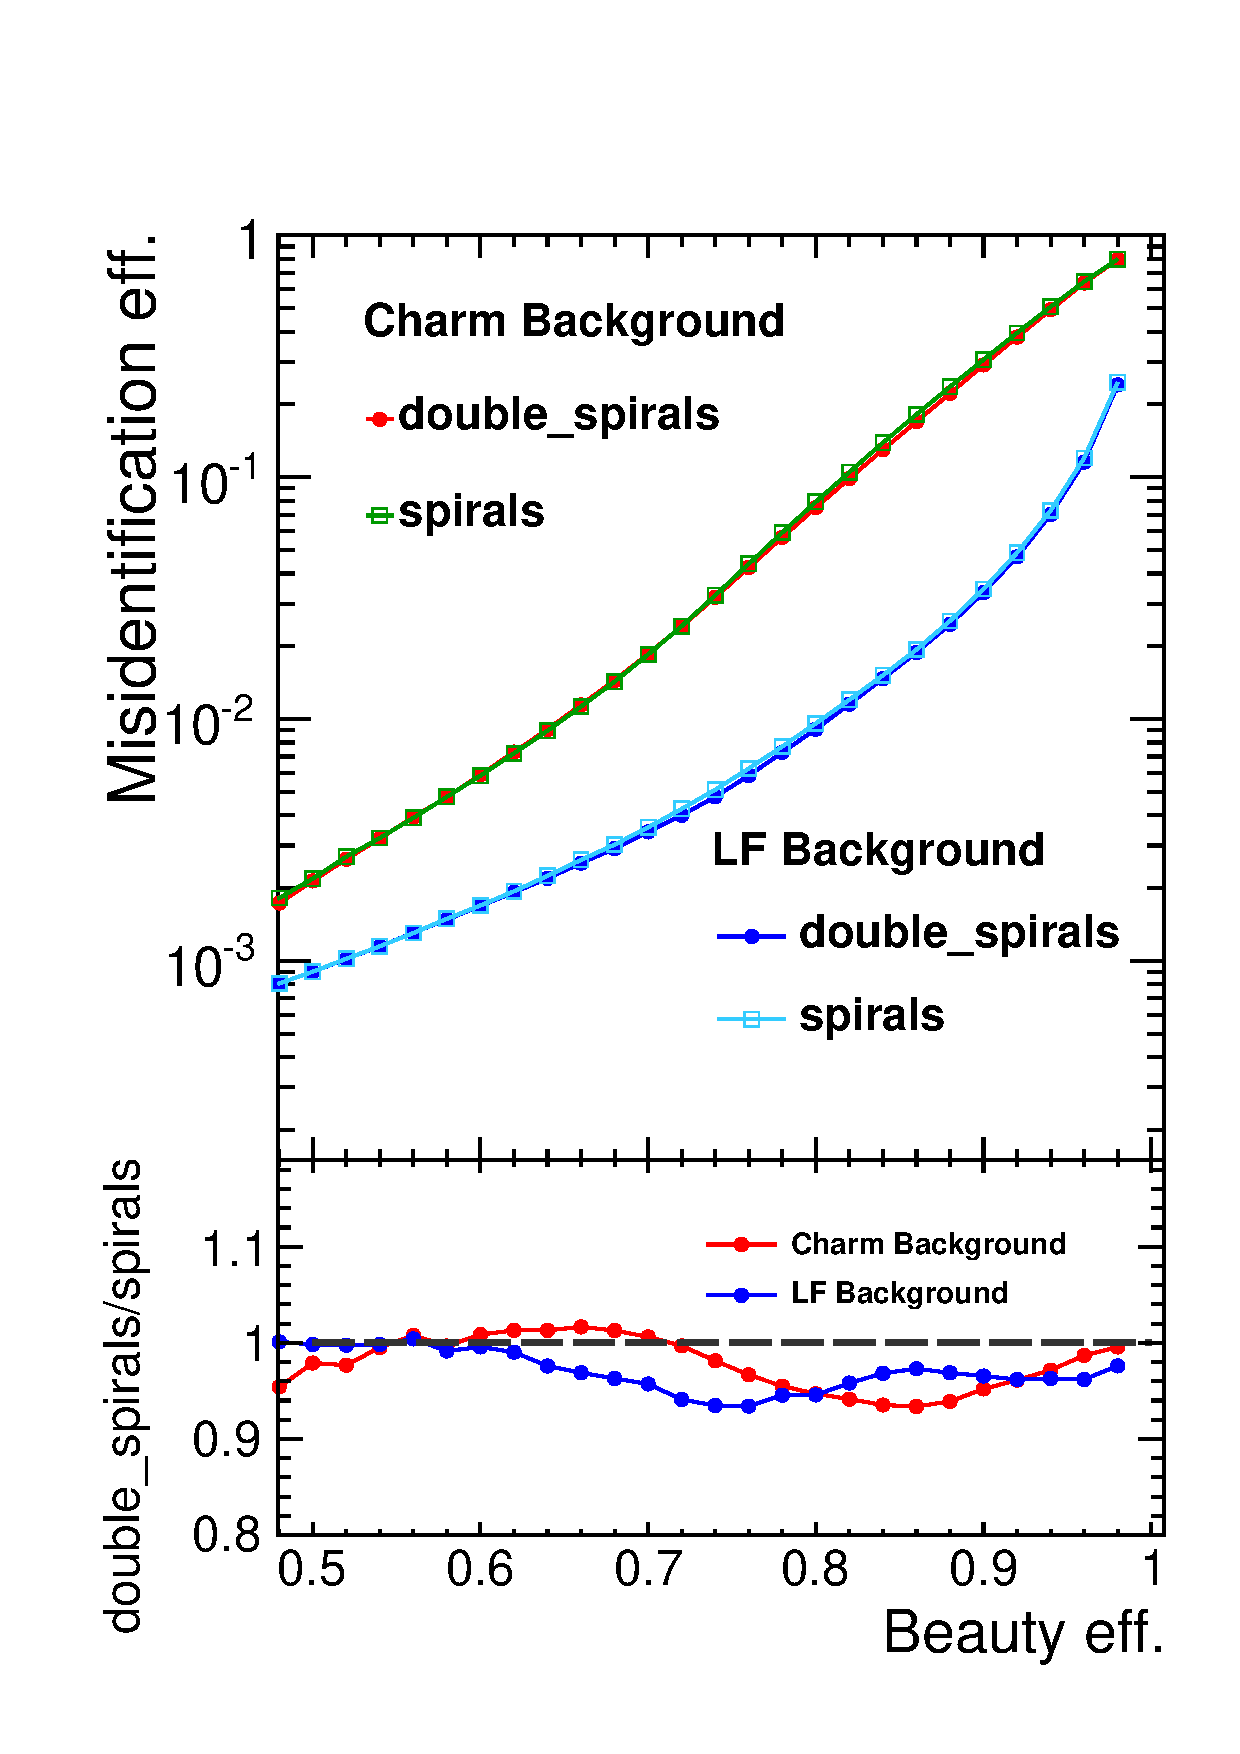
\includegraphics[width=\textwidth]{figures/CLIC/general_200_Beauty.pdf}};
      \draw (1.8, 2.8) node {\textbf{CLICdp}};
    \end{tikzpicture}
    \caption{}
    \label{fig:spiral_doubleSpirals}
  \end{subfigure}~
  \begin{subfigure}[b]{0.33\textwidth}
    \centering
    \begin{tikzpicture}
      \node[anchor=south west, inner sep=0] (image) at (0,0){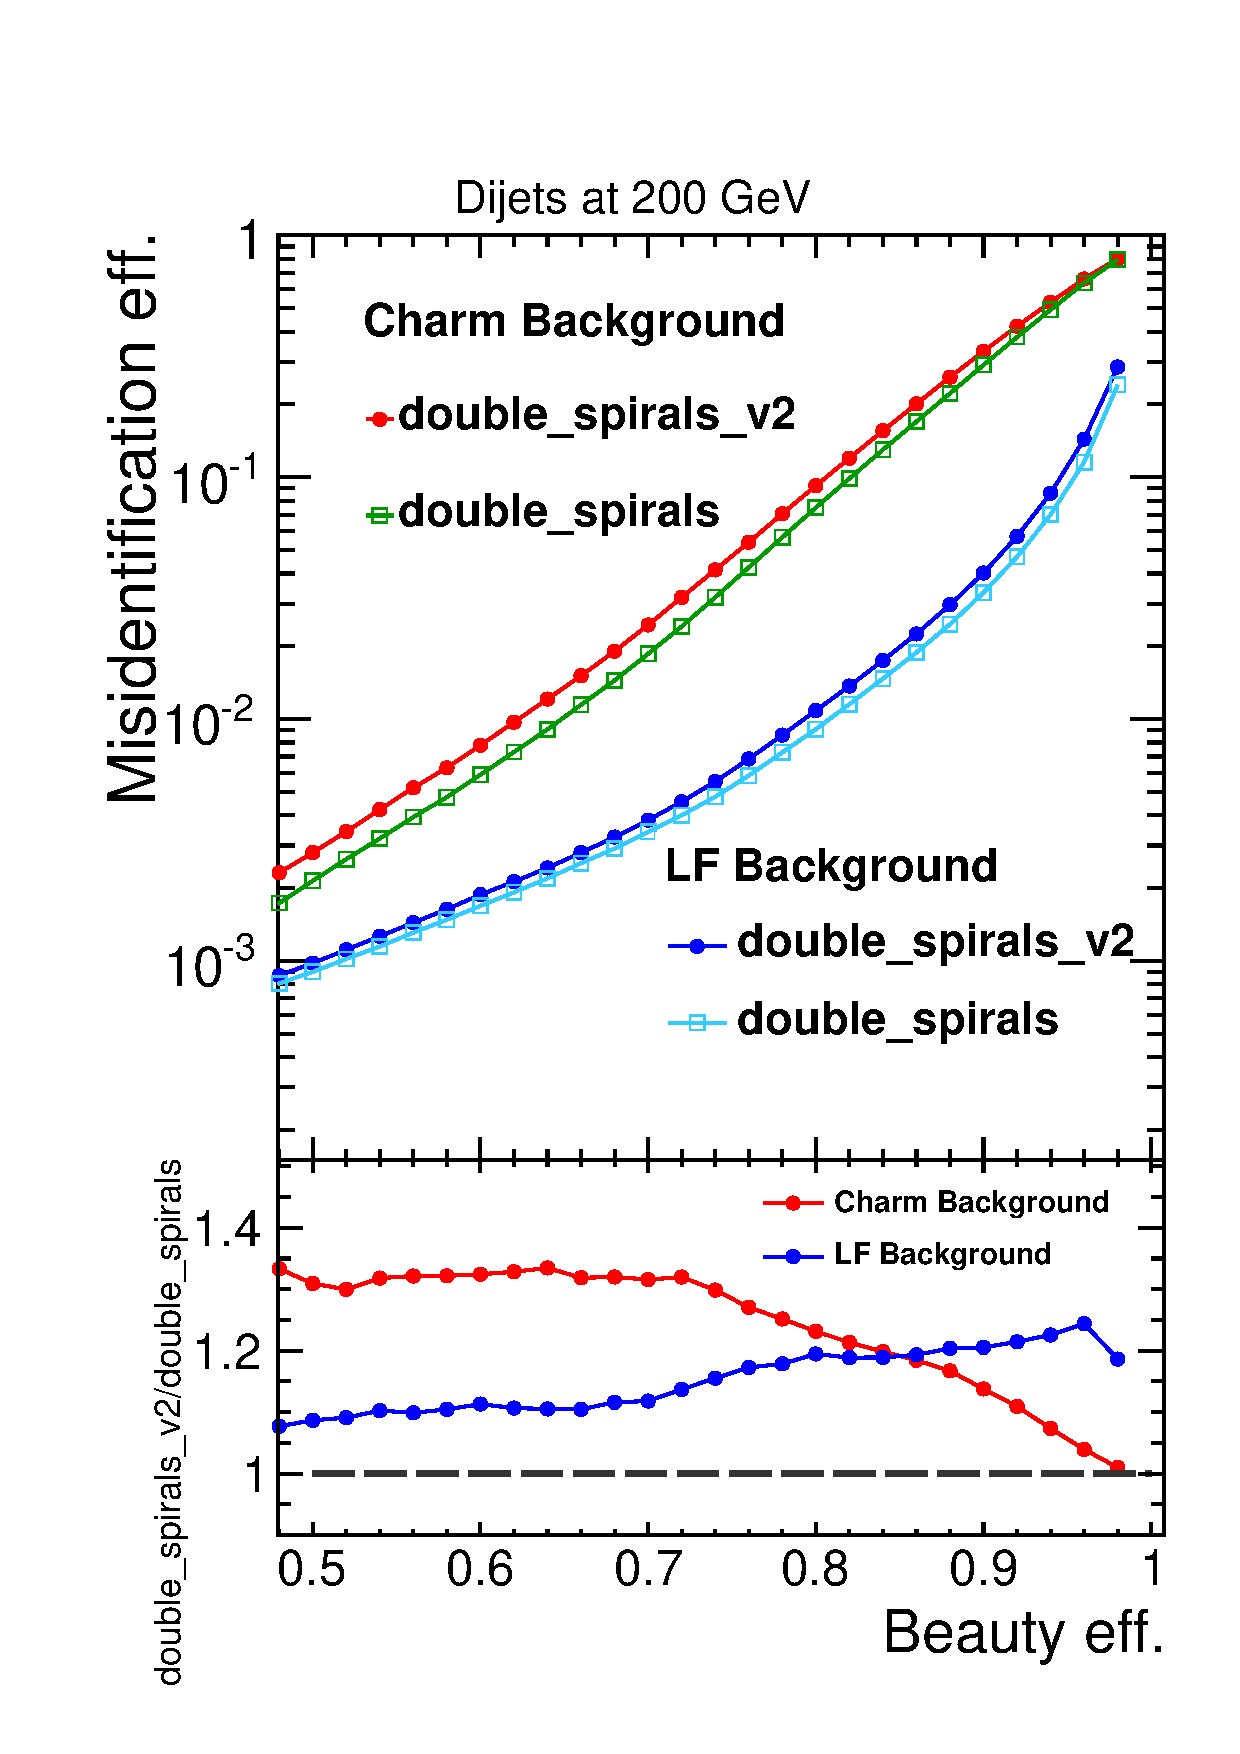
\includegraphics[width=\textwidth]{figures/CLIC/heavy_general_200_Beauty.pdf}};
      \draw (1.8, 2.8) node {\textbf{CLICdp}};
    \end{tikzpicture}
    \caption{}
    \label{fig:doubleSpirals_doubleSpirals}
  \end{subfigure}
  \caption{Beauty-tagging performance for dijet events at
    \SI{200}{\giga\electronvolt}. (a)~Comparison between \emph{disks}
    and \emph{spirals} in terms of the ratio of the misidentification
    probabilities for charm background. (b)~Comparison of the
    beauty-tagging performance between the \emph{spirals} and
    \emph{double\_spirals} geometries. (c)~Comparison of the
    beauty-tagging performance between the \emph{double\_spirals} and
    \emph{double\_spirals\_v2} geometries. For (a) the
    misidentification ratio for each polar angle is shown
    separately. For (b) and (c), dijet events with a mixture of polar
    angles between \SI{10}{\degree} and \SI{90}{\degree} are
    considered. From~\cite{Tehrani:2015tla}.}
  \label{fig:performance}
\end{figure}

A detector model for CLIC is under development which takes into
account the progressing engineering studies. The spiral arrangement of
the modules in the vertex endcaps allows to use airflow cooling which
has the potential to reduce the material budget
significantly. Double-sided modules provide more sensitive layers with
the same amount of support material as single-sided modules. The
overall results show that the implemented geometries are similar in
terms of the flavour-tagging performance for simulated dijet
events. The impact of a spiral arrangement of the modules in the
endcap region remains similar to the disks. The amount of material, on
the other hand, was found to have a large impact on the performance.

The following chapters focus on the R\&D of the pixel detectors in the
vertex detector with high-resolution and very low material budget in
order to achieve high flavour-tagging performance as required by the
precision physics to be measured at CLIC.



% \section{Summary}
% \label{sec:summary_CLIC}

% The CLIC detector model for simulations is under development with the
% requirements set by the precision physics to be measured. With these
% requirements, it allows for identification of beauty and charm quarks
% and this is possible with a vertex detector with a high spatial
% resolution and very low material budget to limit the multiple
% scatterings. This thesis focuses on the R\&D of the pixel detectors in
% the vertex detector with high-resolution and very low material budget.

% ============================================================================== 
% planning for the chapter
% ============================================================================== 
% Accelerator (two-beam acceleration), CLIC detector concept, picture of
% the full detector (3 pages)

% \section{Requirements for the CLIC vertex detector}
% motivation for pixel detectors in high-energy physics (flavour-tagging
% plots), requirements, design, technical challenges
% (cooling/mechanics), Beam induced backgrounds, Radiation damage in the
% vertex detector (3 pages).


% \section{Flavour tagging at CLIC}
% say motivation of this thesis $\Rightarrow$ provide input for the
% digitiser (1 page) and the detector simulation software.

% ==============================================================================
\chapter{Semiconductor detectors}
\label{sec:SiliconTheory}
%==============================================================================    

Semiconductor materials have a great advantage in many radiation
detection applications. The main benefits are the high energy
resolution due to the large number of free charge carriers that are
created by a given incident radiation, their compact sizes, fast
timing, while the effective thickness can be adapted to the
requirements of the applications. Though, they show some limitations
for smaller sizes and their performance can degrade from radiation
induced damages. Among semiconductor materials, silicon detectors are
predominant for charged particle spectroscopy.

In this chapter, we will review the basic properties of semiconductor
material, charge generation in silicon and the transport of charge
carriers through drift and diffusion. Pixel detectors are studied
through pn-junctions. 

%% --------------------------------------------- %%
\section{Basic properties of semiconductor material}
Due to the periodic lattice of crystalline structure of semiconductor
material, electrons within the solid have allowed energy bands. The
energy of the electrons is confined to one of the energy bands and the
bands may be separated by gaps of forbidden
energies.\\ \cref{fig:energyBands} schematically illustrates the bands
in insulators, semiconductors and metals. In the \textit{valence
  band}, the electrons are bonded to specific lattice sites within the
crystal. The electrons in the \textit{conduction band} are free to
move through the crystal and contribute to the electrical
conductivity. The \textit{bandgap} (E\textsubscript{g}) separates the
valence from the conduction band and allows to classify wether the
material is a semiconductor, an insulator or a metal. In the absence
of thermal excitation, the valence band for the semiconductors and
insulators is completely full and the conduction band empty. Therefore
they are not electrically conductive. Metals are highly electrically
conductive since the fermi energy level (E\textsubscript{F}) lies in
the conduction band and the electrons are free to migrate through the
material even at very low temperatures. However, for insulators and
semiconductors the electrons must cross the bandgap to become
conductive. The bandgap for semiconductors ($\sim1\,\ev$) is much
lower than for insulators ($\sim5\,\ev$). If an electron in the
valence band gains enough thermal energy to cross the bandgap and
reach the conduction band, it leaves behind a vacancy (a hole) behind
in the valence band. The electron-hole pair can move under the
influence of an external electric field (electrons in the opposite
direction of the holes). This motion creates conductivity in the
material. This property is exploited in silicon detectors to detect
radiation and is developed more in the coming sections.




\begin{figure}[htbp]
  \centering
  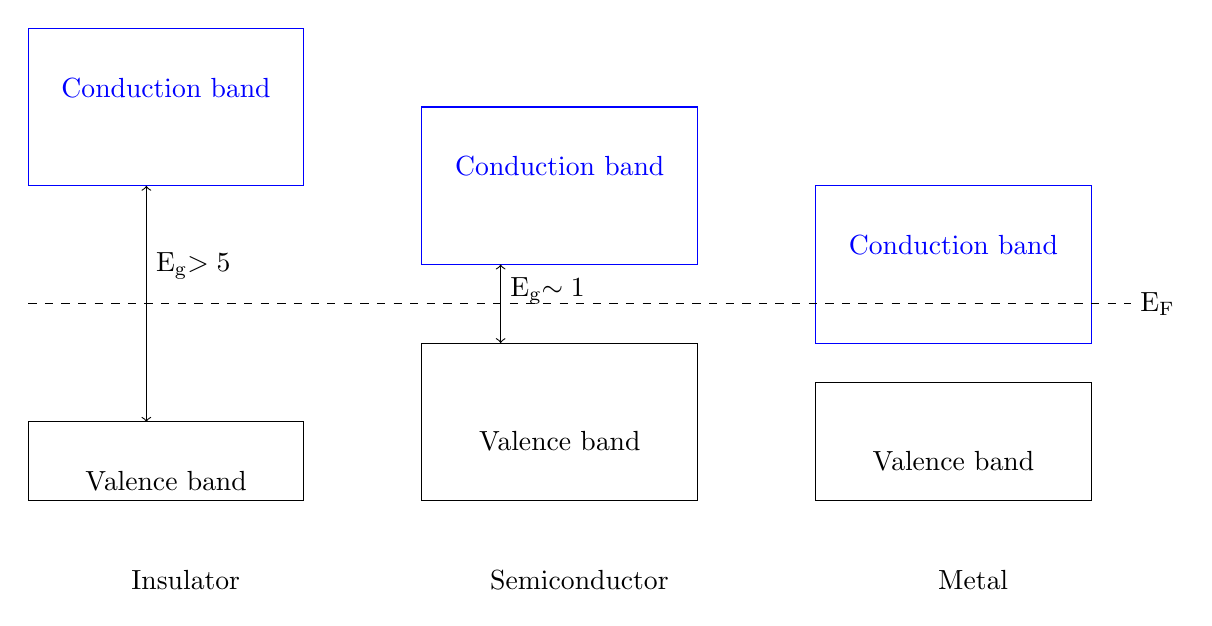
\begin{tikzpicture}
    \begin{scope} % Valence and conduction bands
      %  ----- insulator ----- %
        \draw (0, 1) rectangle node[below] {Valence band}  ++ (3.5, 1);
        \draw[blue] (0, 5) rectangle node[above] {Conduction band} ++ (3.5, 2);
        \node at (2, 0) {Insulator};

        % ----- Semiconductor ----- %
        \draw (5, 1) rectangle node[below] {Valence band}  ++ (3.5, 2);
        \draw[blue] (5, 4) rectangle node[above] {Conduction band} ++ (3.5, 2);
        \node at (7, 0) {Semiconductor};

        % ----- Metal ----- %
        \draw (10, 1) rectangle node[below] {Valence band}  ++ (3.5, 1.5);
        \draw[blue] (10, 3) rectangle node[above] {Conduction band} ++ (3.5, 2);
        \node at (12, 0) {Metal};
    \end{scope}


    \begin{scope} % Energy levels
        \draw[dashed] (0, 3.5) -- (14, 3.5) node[right] {E\textsubscript{F}};
        \draw[arrows=<->](1.5, 2)--(1.5, 5) node [pos=0.66,right] {E\textsubscript{g}$>5\,\ev$};
        \draw[arrows=<->](6, 3)--(6, 4) node [pos=0.66,right] {E\textsubscript{g}$\sim1\,\ev$};
    \end{scope}

  \end{tikzpicture}
  \caption{Illustation of the band structures for electron energies in
  insulators, semiconductors and metals. E\textsubscript{F} represents the Fermi energy level and E\textsubscript{g} the bandgap.}  
  \label{fig:energyBands}
\end{figure}

%% --------------------------------------------- %%
\subsection{Silicon}
\label{sec:silicon}

In semiconductors, the excitation energy is defined by the periodicity
of the crystal lattice. Silicon is a semiconductor with a
\textit{diamond} lattice as illustrated in
\cref{fig:SiliconDiamondLattice}. The dimension $a$ is the lattice
constant and is \SI{5.34}{\angstrom} in silicon.


\begin{figure}[htbp]
  \centering
  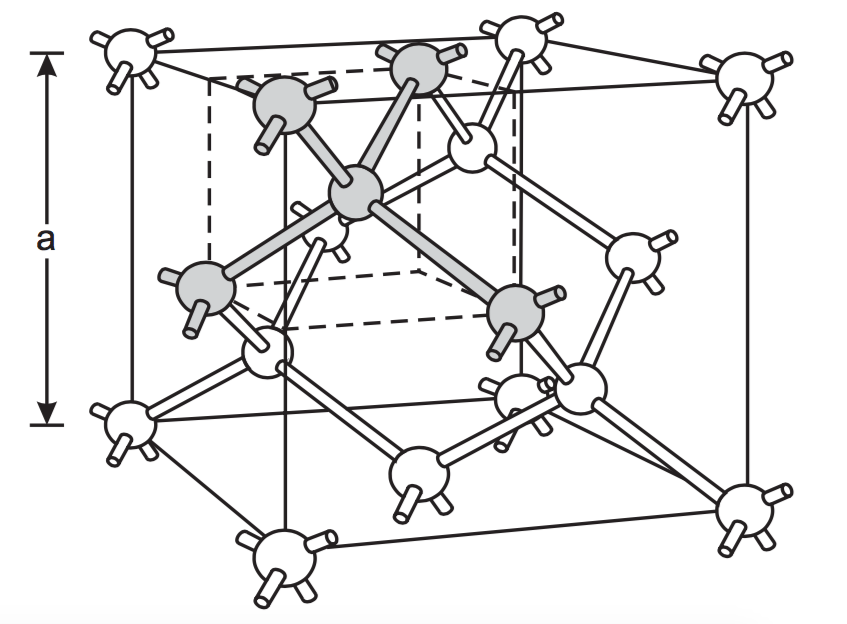
\includegraphics[width=0.5\textwidth]{figures/ChargeSharing/SiliconDiamondLattice.png}
  \caption{Lattice structure of silicon. The building block of the
    lattice is formed by a central atom bonded to four equidistant
    neighbours as shown in shaded
    gray. From~\cite{Spieler2005}.}\label{fig:SiliconDiamondLattice}
\end{figure}

In the periodic table, silicon is a group four element as it has four
valence electrons and which combine with four neighbours to build
covalent bonds and close the outer shell.  At 0~K, no electrical
conduction is possible since all the electrons fill completely the
valence band. An incident radiation can break a bond and excite an
electron into the conduction band. This leaves a \textit{hole} or a
vacant state in the valence band and the electron can freely move in
the conduction band. The hole can also move in the valance band by the
indirect mechanism where an electron from a neighbouring atom fills it
and creates another hole.

An external electric field can direct the motion of the electrons and
holes created. Holes are treated as positive charge carriers. 

In silicon, the ionisation energy or the average energy deposition
required to produce an electron-hole pair is $3.6\,\ev$.

%% --------------------------------------------- %%
\subsection{Doping}
\label{sec:doping}

By introducing special impurities, the conductivity of semiconductors
can be controlled. Typical concentration ranges between
$10^{12}-10^{18}\,\inversecmcubic$. In semiconductors, the
conductivity comes from either electrons (n-type) or holes (p-type).

In \textit{n-type doping}, a silicon atom is replaced with an atom
having five valence electrons, for example phosphorus. This creates an
excess in electrons into the lattice and is called a donor. The donor
electron is lightly bound to the impurity atom. As a consequence, the
ionisation probability is increased and mobile electrons are
introduced into the conduction band.

In \textit{p-type doping}, by introducing a group three atom into the
silicon lattice such as the boron, one impurity valence electron is
left. This type of dopant is called an acceptor: the dopant borrows an
electron from a neighbouring atom and the holes can move freely
throughout the crystal.
 
%% --------------------------------------------- %%
\section{Charge generation and recombination in silicon}
\label{sec:chargeInSi}

Previously, we have reviewed the basic properties of semiconductor
material with a focus on silicon. The electron-hole generation is also
introduced. In this section, we focus on the amount of charge
generated due to an incident radiation.

\subsection{Bethe-Bloch formula}
In silicon, free charge careers are generated due to thermal effects
and lead to leakage current. A current is also generated due to the
interaction of charged particles with silicon and can be
detected. Part of the absorbed energy generates electron-hole pairs
through scattering processes with the shell electrons of silicon and
can be collected by the readout electronics. The number of
electron-hole pairs produced, as well as the total energy loss of the
particle in the detector, are stochastic quantities.

The energy loss along the particle track is described by the
Bethe-Bloch formula~\cite{Beringer:1900zz}:

\begin{equation}
  - \braket{{dE}\over{dx}} = 4 \pi N_A r_{e}^2 m_e c^2 z^2 \frac{Z}{A}  \frac{1}{\beta^2} \left[ \frac{1}{2} \ln{\frac{2 m_e c^2 \beta^2 \gamma^2 T_{max}}{I^2}} - \beta^2 - \frac{\delta\left(\beta\gamma\right)}{2}\right]\; ,
  \label{eq:BetheBloch}
\end{equation}

where $N_A$ is the Avogadro's number, $r_e$ the classical electron
radius, $m_ec^2$ the rest energy of the electron, $z$ is the charge of
the traversing particle, $Z$ the atomic number, $A$ the atomic mass of
the absorption medium, $\beta={v \over c}$,
$\gamma=1/\sqrt{1-\beta^2}$, $I$ the mean excitation energy, $T_{max}$
the maximum kinetic energy that a particle can transfer to a shell
electron and $\delta\left(\beta\gamma\right)$ the density effect
correction to ionisation energy loss. Relativistic particles with an
energy loss near the minimum of the Bethe-Bloch formula are considered
as minimum ionising particles (MIPs).

\subsection{Energy-loss spectrum in silicon}
Ionisation is also subject to statistical fluctuations and
\cref{eq:BetheBloch} gives its average value. It can be described by a
probability density function called \textit{straggling function} and
characterised by the most probable energy loss ($\Delta_{p}$) and
full-width-at-half-maximum ($w$). \cref{fig:LandauDistribution} shows
examples of this distribution in thin sensors. If a particle is not
stopped in the sensor, the energy deposition varies around the peak of
the distribution with a large tail for high signals. The main reason
for the highly-skewed energy-loss distribution is the manifestation of
$\delta$-rays which happens when electrons acquire enough energy by
interaction and themselves become ionising particles. The
$\delta$-rays not only make the average value of the energy-loss
higher than the most probable value ($\Delta_{p}$) of the
distribution, but also create big clusters and thus degrade the
spatial resolution of the detector. This is the reason why the Bethe
equation (c.f. \cref{eq:BetheBloch}) is ill-defined experimentally and
not used for applications where the energy loss for single particles
is described.

The fluctuations around $\Delta_{p}$ increase for thinner sensors and
should be taken into account for the design of the dynamic range of
the readout electronics.


\begin{figure}[htbp]
  \centering
  \includegraphics[width=0.7\textwidth, page=14, trim = 50mm 160mm
    40mm 20mm, clip]{Articles/rpp2009-rev-passage-particles-matter.pdf}
  \caption{Straggling function in silicon for 500 MeV pions,
    normalized to unity at the most probable value $\Delta_{p}$. $w$
    is the full-width-at-half-maximum~\cite{Beringer:1900zz}.}
  \label{fig:LandauDistribution}
\end{figure}

In literature, several approaches address the calculation of the
straggling functions. The Landau and the Bichsel models, two of the
most relevant models, are described in \cref{sec:landau,sec:bichsel}. 

The probability of the occurrence of collisions and the probability
for a particular energy loss $E$ are considered for the calculation of
the straggling functions. To obtain correct straggling functions, the
accurate determination of the collision cross section as function of
energy loss, $\sigma(E)$, is necessary.

\subsection{The Landau distribution}\label{sec:landau}
The most commonly used model in experiments, is a Landau distribution
convoluted with a Gaussian. The most probable value $\Delta_p$ of the
distribution is given by the Landau-Vavilov
method~\cite{Landau:1944if,Vavilov:1957zz}:

\begin{equation}
  \Delta_p=\xi \left[\text{ln}{{2mc^2\beta^2\gamma^2}\over{I}}+\text{ln}{\xi \over I}+0.200-\beta^2-\delta\left(\beta\gamma\right) \right] \; ,
  \label{eq:LandauVavilovMPV}
\end{equation}

where $\xi=(K/2)\braket{Z/A}(x/\beta^2)$~\mev for a detector of
moderate thickness $x$ in g~\inversecmsquared. All the other
parameters are similar to the ones described for \cref{eq:BetheBloch}.

Though the Landau-Vavilov calculation does not describe correctly the
width of the energy distribution for thin silicon sensors. For thick
material, the width of the distribution is $4\xi$.

For $\gamma\gg100$, \cref{eq:LandauVavilovMPV} is simplified to~\cite{Bichsel}

\begin{equation}
  \textsubscript{L}\Delta_{p} (\kev)=t \left(0.1791+0.01782 \ln\left(t\right)\right) \; ,
  \label{eq:LandauVavilovMPV_simplified}
\end{equation}

where $t$ (in \micron) is the thickness of the silicon.

When the Landau distribution is combined with a Gaussian, $\Delta_ p$
increases and gives better agreement with data.

\subsection{The Bichsel model}\label{sec:bichsel}
The Bichsel model~\cite{Bichsel} takes into account the binding of
atomic electrons to find a better agreement between data and
theory. In this model, experimental and theoretical data for
dielectric functions, x-ray absorption coefficients and generalised
oscillator strengths are used to reproduce accurately the observed
energy loss spectrum over a wide range of incident particle velocities
and silicon thicknesses, including very thin silicon sensors. But no
analytical description of the straggling function is provided.

Bichsel provides an approximation of $\Delta_{p}$ and $w$ (in \ev) as
function of the thickness $t$ (in $\micron$) of silicon detectors for
particles with charge $\pm1e$ and $\beta\gamma>500$ as listed in
\cref{eq:MPV1,eq:MPV2,eq:FWHM}:

\begin{itemize}
\item For $13<t<110$ [\micron]:
  \begin{equation}
    \Delta_{p}=t \cdot \left(100.6+35.35 \cdot \ln(t) \right)\; ,
    \label{eq:MPV1}
  \end{equation}
\item For $110<t<3000$ [\micron]:
  \begin{equation}
    \Delta_{p}=t \cdot \left(190+16.3 \cdot \ln(t) \right)\; ,
    \label{eq:MPV2}
  \end{equation}
\item For $30<t<260$ [\micron]:
  \begin{equation}
    w=t \cdot \left(259.6-28.41 \cdot \ln(t) \right).
    \label{eq:FWHM}
  \end{equation}
\item For $260<t<2560$ [\micron]:
  \begin{equation}
    w=71.3 t \left( 1+ 39.4/t^{0.8} \right)
    \label{eq:FWHM2}
  \end{equation}
\end{itemize}

\cref{tab:EdepForDifferentThickness} summarises the $\Delta_{p}$ and
$w$ for detectors thicknesses at our disposal and tested at test beams
with the results presented in the following chapters.

\begin{table}[htbp]
  \centering
  \caption{Calculated $\Delta_{p}$ and $w$ for silicon sensors with
    various thicknesses using
    \cref{eq:MPV1,eq:MPV2,eq:FWHM,eq:FWHM2}.}
  \label{tab:EdepForDifferentThickness}
  \begin{tabular}{c c c c}
    \toprule
    Thickness [\micron] &  $\Delta_{p}$ [\kev] & $w$ [\kev] & $\Delta_{p} / w$ \\ 
    \midrule
    50 & 11.9 & 7.42 & 1.6      \\
    100 & 26.34 & 12.88 & 2.045 \\
    150 & 40.75 & 17.59 & 2.32  \\
    %%200 & 55.27 & 21.82 & 2.53  \\
    300 & 84.89 & 30.18 & 2.8 \\
    \bottomrule
  \end{tabular}
\end{table}

\subsection{Multiple scattering}

In addition to energy loss, when a particle goes through the detector,
its trajectory is deflected by small-angle scatters. The deflection is
mainly due to the Coulomb interaction of the charged particle with the
nuclei. The strong interaction has also a contribution for
hadrons. When leaving the detector, the scattering angle of the
particle follows a Gaussian distribution with an RMS given
by~\cite{Lynch:1990sq}:

\begin{equation}
  \theta\textsuperscript{RMS}={{13.6\,\mev}\over{\beta p c}} z
\sqrt{x \over X_0} \left[1+0.038\ln{\left(x \over X_0 \right)}\right],
  \label{eq:multipleScattering}
\end{equation}

where the angle $\theta$ is in radians, the particle momentum $p$ in
\mev, $z$ the charge number of the particle and $x/X_0$ the thickness of
the absorption medium in units of the radiation length.

In high-energy physics applications, the material budget of pixel
detectors is minimised in order to have the smallest scattering angles
possible.

%% --------------------------------------------- %%
%% \subsection{\textsc{Geant4}}\label{sec:Silicon_Geant4}
%% --------------------------------------------- %%
\section{Silicon device physics and properties}


In this section, we review the motion of the charge carriers in
silicon. First the motion in an intrinsic silicon is studied. Then, a
pn-junction is described and the motion of charge carriers in silicon
detectors is sketched.

\subsection{Transport of charge carriers}
In silicon detectors, the movement of the charge carriers (holes and
electrons) lead to signal pulses in the electrical contacts which can
be detected by the readout electronics. 
In the absence of any external electric field, free charge carriers move
randomly and are scattered due to their collisions with the crystal
lattice or other impurities. On average, in equilibrium conditions,
the traveled distance averaged over charges is zero. In addition to
the statistical movement, two other mechanisms can affect the
transport of charge carriers: diffusion (due to a gradient in
concentration) and drift (in the presence of an external electric
field).

The diffusion implies that a carrier is more probable to move from a
high-concentration region to a low-concentration region. The diffusion
current per unit area is given by~\cite{Rossi:976471}:

\begin{equation}
  \begin{aligned}
    J_{n, diff}=-{kT \over e} \mu_n \nabla n \qquad \textnormal{for electrons}
    \; , \\
    J_{p, diff}={kT \over e} \mu_p \nabla p \qquad \textnormal{for holes}
    \; , 
  \end{aligned}
  \label{eq:diffusionCurrent}
\end{equation}
where $k$ is the Boltzmann constant, $T$ the absolute temperature, $e$ the
elementary charge, $\mu$ the mobility of the charge carriers, $\nabla
n$ and $\nabla p$ are the gradients of the electron and hole
concentrations.

Charge carriers are accelerated between two random collisions in the
presence of an external electric field in the direction of the field
and leads to and average drift velocity given by~\cite{Rossi:976471}:

\begin{equation}
  \begin{aligned}
    v_{n}=-\mu_n \textbf{E} \qquad \textnormal{for electrons}
    \; , \\
    v_{p}=\mu_p \textbf{E} \qquad \textnormal{for holes}
    \; , 
  \end{aligned}
  \label{eq:driftVelocity}
\end{equation}
where $v$ is the average drift velocity, $\textbf{E}$ the electric
field and $\mu$ the mobility of the charge carriers. The mobility is a
function of the electric field. For higher electric fields the charge
carriers gain more acceleration and the number of collisions per unit
time increases. This leads to a saturation of the drift velocity
$v_s$. The mobility dependence on the electric field is described by~\cite{Jacoboni197777}:
\begin{equation}
  \mu=\frac{v_{s}/E_{c}}{\left[1+(E/E_{c})^{\beta}\right]^{1/\beta}}\; ,
  \label{eq:mobility}
\end{equation}

where the parameters are described in \cref{tab:mobility_parameters}.

\begin{table}[htbp]
  \centering
  \caption{Parameters for the mobility as described in
    \cref{eq:mobility} with T the absolute temperature and E the
    absolute electric field.}
  \label{tab:mobility_parameters}
  \begin{tabular}{c c c c}
    \toprule
    Parameter & Electrons & Holes & unit \\
    \midrule
    $v_s$ & 1.53 $\times$ $10^9$ $\times$ T\textsuperscript{-0.87} &
1.62 $\times$ $10^8$ $\times$ T\textsuperscript{-0.52} & cm/s \\ 
    $E_c$ & 1.01 $\times$ T\textsuperscript{1.55} & 1.24 $\times$ T\textsuperscript{1.68} & V/cm \\ 
    $\beta$ & 2.57 $\times$ $10^{-2}$ $\times$ T\textsuperscript{0.66} & 0.46 $\times$ T\textsuperscript{0.17} & -\\
    \bottomrule
  \end{tabular}
\end{table}

\cref{fig:Mobility_electron_holes} shows the mobility for electrons
and holes as a function of the electric field. For a low electric
field, the mobility for intrinsic silicon at 300~K is:
\begin{equation*}
  \begin{aligned}
    \mu_n=1415 \pm 46 \qquad \textnormal{\cmsquared/(Vs)} \; , \\
    \mu_p=480 \pm 17 \qquad \textnormal{\cmsquared/(Vs)} \; .
  \end{aligned}
\end{equation*}

\begin{figure}[htbp]
  \centering
  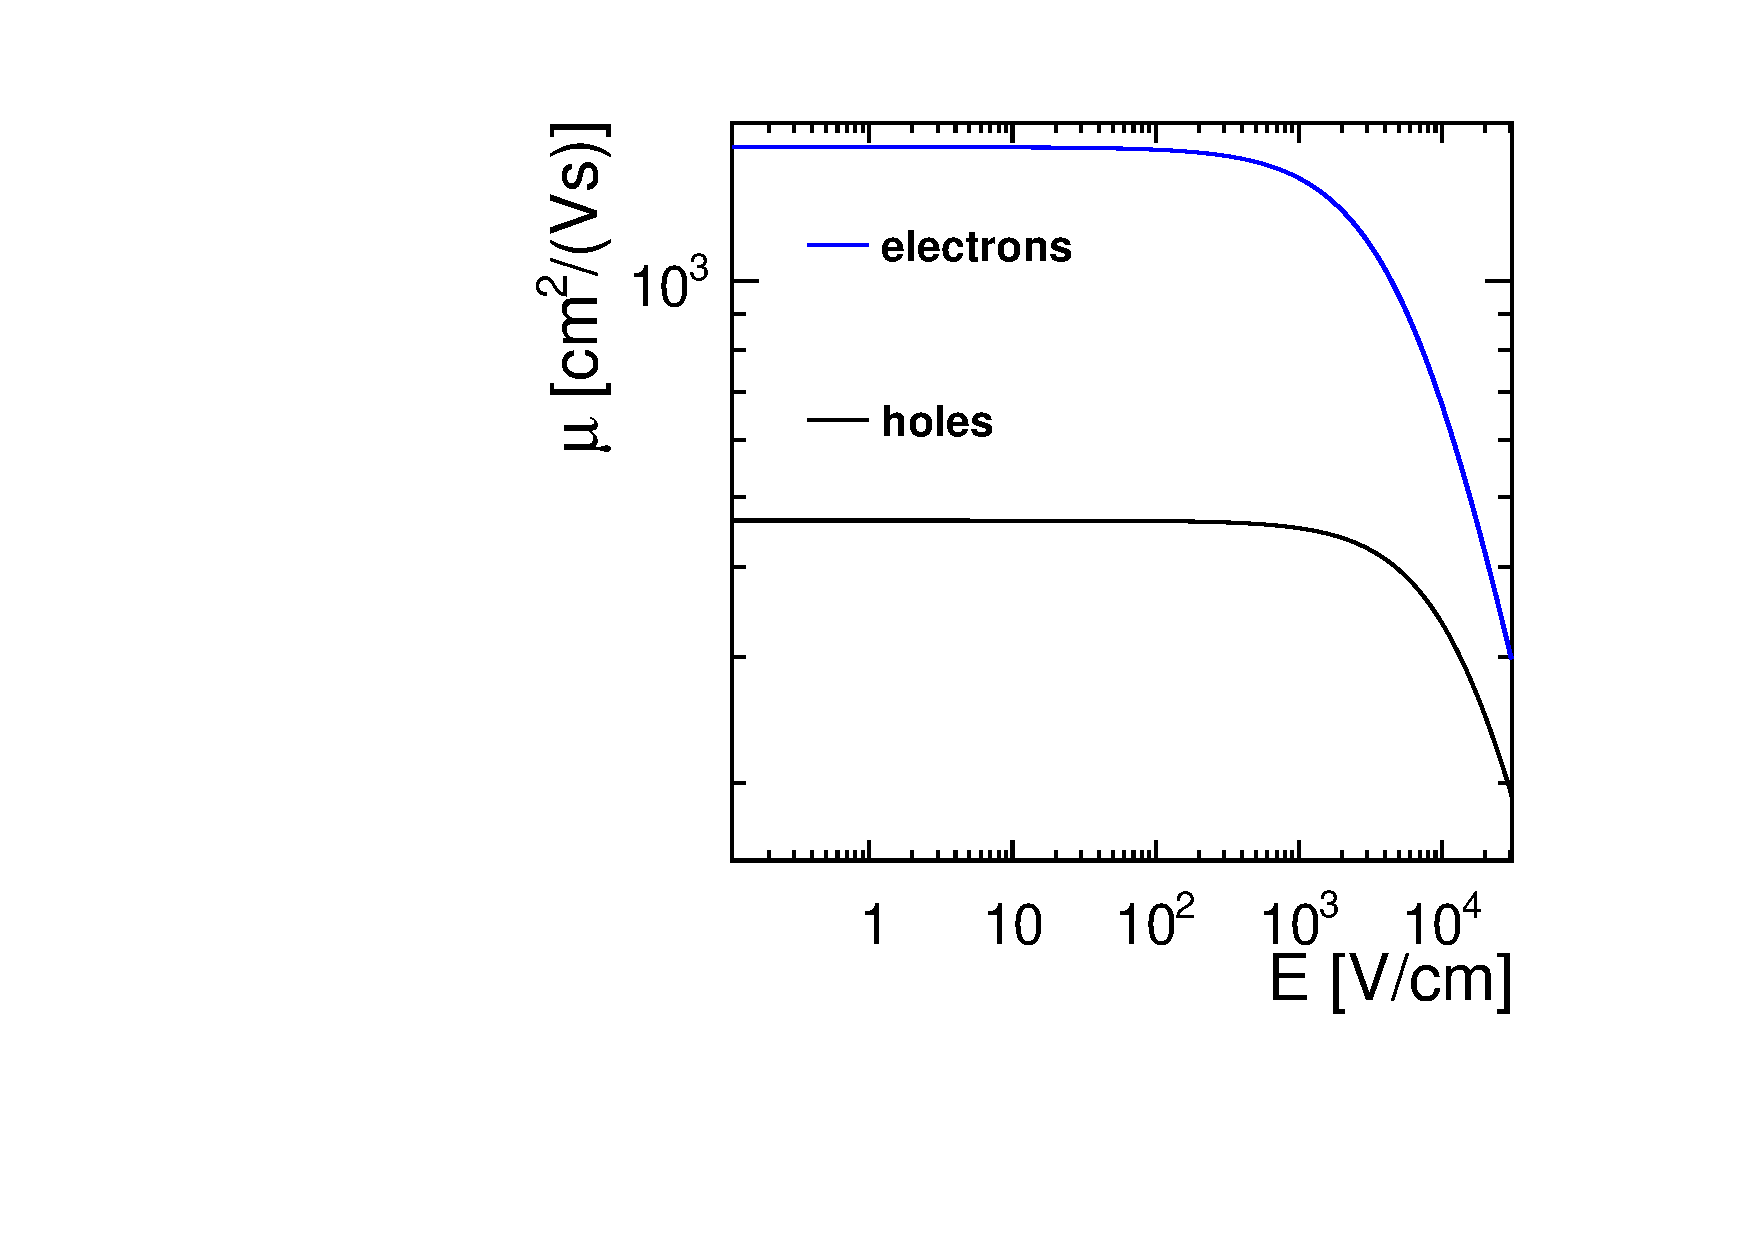
\includegraphics[width=0.5\textwidth]{figures/ChargeSharing/Mobility_electron_holes.pdf}
  \caption{Mobility for electrons and holes as a function of an
    applied electric field calculated with the \cref{eq:mobility}.}
  \label{fig:Mobility_electron_holes}
\end{figure}


Holes are three times less mobile than electrons which make them more
likely to be trapped in an irradiated material.

%% --------------------------------------------- %%
%\section{Pixel detectors: pn-junction}

% Silicon sensors are made of reversely biased pn-junctions. The
% electric field due to the bias voltage allows the charge carriers to
% drift towards the readout chip and also to suppress the leakage
% current.

\subsection{pn-junction in thermal equilibrium}

By joining a p-type with an n-type material, a pn-junction is
obtained. The p and n-type regions are electrically neutral. Due to
thermal diffusion, the holes and the electrons are driven across the
junction. This implies that electrons move from the n-type material to
the p-regions leaving a positive net charge in n-regions. The same
applies to the p-type region which is negatively charged. A potential
is built up when the electrons diffuse to the p-region. This potential
limits the diffusion depth when it exceeds the available energy for
thermal diffusion and is called the built-in potential $V_{bi}$
between the p and n-regions. The built-in potential depends
logarithmically on the doping levels~\cite{Spieler2005}:

\begin{equation}
  V_{bi}= {{kT}\over e} \text{log}\left({N_a N_d} \over {n_i^2} \right)\; ,
  \label{eq:Built_in_potential}
\end{equation}

where $N_a$ and $N_d$ are the acceptor and donor concentrations and
$n_i$ is the intrinsic silicon carrier concentration. For a typical
detector diode $V_{bi}\approx0.5$~V.

The diffusion of the holes and electrons across the junction to the
oppositely-doped regions, leads to a region free of mobile carriers
called the depletion region. As seen previously, $V_{bi}$ limits the
diffusion depth and therefore the width of the depletion region.

Applying an external potential breaks down the thermal equilibrium. By
applying a reverse bias potential, i.e. negative potential to the
p-region and positive potential to the n-region, the potential barrier
and the depletion width are increased.

Under a forward bias on the pn-junction, the diode current increases
rapidly with the voltage. But a reverse bias causes a quick
saturation of the current flow within the junction and the pn-diode
can be used as a rectifier. This property is used for the detection of
radiation in silicon detectors as described in the next section.

\subsection{reverse-biased pn-junction}

The reverse-biased pn-junction is crucial in detection of radiation in
silicon detectors as it increases the depletion width. This forms a
capacitor empty of charge carriers where the undepleted p and
n-regions are the electrodes and the depletion region is the
dielectric. The electric field in the depletion region the mobile
carriers to the electrodes.  The electric field due to the bias
voltage allows the charge carriers to drift towards the readout chip
and also to suppress the leakage current which can be an important
source of noise.

Here, we derive the depletion width, the electric field distribution,
the drift and the diffusion within a pn-junction reverse-biased at a
voltage of $V_B$.

The potential $\varphi$ at each point is described by Poisson's
equation~\cite{Knoll2010}:

\begin{equation}
  \nabla^{2}  \varphi=-{\rho \over \epsilon}\; ,
  \label{eq:poisson}
\end{equation}

where $\epsilon$ is the dielectric constant of the medium and $\rho$
the net charge density. The electric field E due to the electric
potential is obtained by:

\begin{equation}
E=-\text{grad }\varphi \; .
\label{eq:Efield}
\end{equation}


To simplify, we assume an abrupt junction where the charge densities
on the p and n-regions illustrated in \cref{fig:chargeDensity} and
given by:
\begin{equation}
  \rho(z)= 
  \begin{cases} 
    eN_{d}, & \mbox{if } 0\leq z < z_{n}\\ 
    -eN_{a}, & \mbox{if } z_{p}\leq z < 0 
  \end{cases} 
  \; .
\label{eq:chargeDensity}
\end{equation}

\begin{figure}[htbp]
  \centering
  \begin{tikzpicture}[node distance = 2.5cm, auto]
    \begin{scope}[x={(image.south east)},y={(image.north west)}]

      \draw[black, thick, ->] (0.5, 0.1) -- (0.5, 0.9); 
      \node[above, color=black] at (0.5, 0.9) {$\rho$};
      \draw[black, thick, ->] (0.1, 0.5) -- (0.9, 0.5);
      \node[right, color=black] at (0.9, 0.5) {Depth (z)};
      \node[left, color=black] at (0.5, 0.6) {e$N_d$};
      \node[below, color=black] at (0.8, 0.5) {$z_n$};

      \node[above, color=black] at (0.3, 0.5) {$z_p$};
      \node[right, color=black] at (0.5, 0.2) {-e$N_a$};
      
      \draw[black, thick, dashed] (0.5, 0.6) -- (0.8, 0.6); 
      \draw[black, thick, dashed] (0.8, 0.6) -- (0.8, 0.5);
 
      \draw[black, thick, dashed] (0.3, 0.5) -- (0.3, 0.2);
      \draw[black, thick, dashed] (0.5, 0.2) -- (0.3, 0.2);

      % \draw[help lines,xstep=.1,ystep=.1] (0, 0) grid (1,1);
      % \foreach \x in {0,1,...,9} { \node [anchor=north] at (\x/10,0) {0.\x}; }
      % \foreach \y in {0,1,...,9} { \node [anchor=east] at (0,\y/10) {0.\y}; }

    \end{scope}
  \end{tikzpicture}
  \caption{Charge density distribution for a simplified pn-junction.}
  \label{fig:chargeDensity}
\end{figure}



In one dimension, Poisson's equation is simplified to:
\begin{equation}
{{d^{2}  \varphi(z)} \over {dz^{2}}}=-{\rho(z) \over \epsilon}\; .
\label{eq:poisson1D}
\end{equation}

First, considering the n-side, the first and second integrations of the Poisson equation give:
\begin{equation}
    {{d\phi(z)} \over {dz}}=-{{eN_{d}} \over \epsilon} (z-z_{n}) 
    \; ,
    \label{eq:PoissonIntegration1}
  \end{equation}

\begin{equation}
  \phi(z)=-{{eN_{d}} \over \epsilon} {z^{2} \over 2}+{{eN_{d}zz_{n}}\over \epsilon}+Vj
  \; ,
  \label{eq:PoissonIntegration2}
\end{equation}

where $V_j$ is the potential at the interface where the n- and the p-sides join. At the boundary of the depletion region $z=z_{n}$:

\begin{equation}
  \phi(z_{n})=V_{B}={{eN_{d}z_{n}^{2}} \over \epsilon}+V_j 
  \; ,
  \label{eq:BounderyPotential}
\end{equation}

where $V_B$ is the reverse bias voltage. In the p-region,

\begin{equation}
  V_j={{eN_az_p^2} \over {2\epsilon}}
  \; .
\end{equation}

The total potential is given by:

\begin{equation}
V_b={{e} \over {2 \epsilon}}(N_dz_n^2+N_az_p^2)
  \; .
\end{equation}

Since the overall charge neutrality is maintained,
\begin{equation}
N_d z_n=N_a z_p
  \; ,
\end{equation}

the reverse bias potential can be expressed as:

\begin{equation}
V_b={e \over {2\epsilon}}\left(1+{N_a \over N_d}\right) N_a z_p^2={e \over {2\epsilon}}\left(1+{N_d \over N_a}\right) N_d z_n^2
  \; .
\end{equation}

The depletion widths on the n- and p-sides of the junction are

\begin{equation}
  \begin{multlined}
z_n=\sqrt{{2 \epsilon V_b} \over {eN_d(1+N_d/N_a)}} \\
z_p=\sqrt{{2 \epsilon V_b} \over {eN_a(1+N_a/N_d)}} 
\; .
\end{multlined}
\end{equation}

The total depletion width is 

\begin{equation}
W=z_n+z_p=\sqrt{{2 \epsilon V_b \left(N_a+N_d\right)} \over {eN_aN_d} }
\; .
\end{equation}

Considering an asymmetrical junction with $N_d \ll N_a$ for which the
junction potential is equal to the potential of the p-contact:

\begin{equation}
V_j=\left(N_d \over N_a\right) {V_b \over \left(  1+N_d/N_a \right)} \stackrel{N_d \ll N_a}{\approx} {N_d \over N_a}V_b
\; .
\end{equation}


For a pixel detector with asymmetric junction with a highly doped
surface $N_c$ concentration and a lightly doped bulk $N_b$
($N_b \ll N_c$), the doping concentration is expressed in terms of the
bulk resistivity,
\begin{equation}
\rho_b = {1 \over {e\mu_{b}N_{b}}}
\; ,
\end{equation}
where $\mu_b$ and $N_b$ are the mobility and the doping concentration
of the bulk. The depletion width $W$ becomes,
\begin{equation}
W=\sqrt{2 \epsilon \mu_b \rho_bV_b}
\; .
\label{eq:depletionWidth}
\end{equation}

By taking into account the built-in reverse bias voltage,
\cref{eq:depletionWidth} is written as,

\begin{equation}
W=\sqrt{2 \epsilon \mu_b \rho_b \left(V_b+V_{bi}\right)}=\sqrt{{2 \epsilon \left(V_b+V_{bi}\right)} \over {eN_b}}
\; .
\label{eq:depletionWidth2}
\end{equation}

The electric field of \cref{eq:PoissonIntegration1}, by replacing the depletion width and $N_d$ by \cref{eq:depletionWidth2} can be expressed as
\begin{equation}
E(z)={{2\left(V_b+V_{bi}\right)} \over {W}} \left({z \over W}-1\right)
\; .
\end{equation}

The depletion voltage (for $W=d$) can be expressed as,
\begin{equation}
V_D={{eN_bd^2} \over {2 \epsilon}}-V_{bi}
\; ,
\label{eq:depletionVoltage}
\end{equation}
where $d$ is the detector thickness. \\

The electric field drops linearly from its maximum value at the
junction to zero at the opposite contact. Increasing the bias voltage
beyond the needed bias to completely deplete the detector adds a
uniform field. By neglecting the built-in voltage (as the bias voltage
is much higher), the electric field is written as,
\begin{equation}
E(z)={{V_B-V_D} \over d}+\left(1-{z \over d}\right)2{V_D \over d}
\; .
\label{eq:Efield_drift}
\end{equation}

The charge carriers, drift through the silicon detector with a
velocity as defined by,

\begin{equation}
  \vec{v}_{drift}=\mu_c \cdot \vec{E}\; .
\end{equation}

In one-dimension, and considering $\mu_c$ constant, the drift velocity is written as
\begin{equation}
v_{drift}={{dz} \over {dt}}=\mu_c \cdot E(z)
\; .
\end{equation}

The time required for a charge originating at point $z_0$ to reach a point $z$ is
\begin{equation} 
  t(z)=\int_{z_0}^{z} {{ds} \over {\mu_c \cdot E(s)}}
  \; .
  \label{eq:driftTimeIntegral}
\end{equation}

By integrating \cref{eq:driftTimeIntegral} and replacing the electric
field by \cref{eq:Efield} one obtains:

\begin{equation} 
  t(z, z_0)={{d^2} \over {2 \mu_c V_D}} ln\left( {{d(V_B+V_D)-2V_Dz_0} \over {d(V_B+V_D)-2V_Dz}} \right)
  \; .
  \label{eq:driftTimeIntegratedz0}
\end{equation}

In \cref{eq:driftTimeIntegratedz0}, by replacing $z_0=0$, we obtain:
\begin{equation} 
  t(z)={{d^2} \over {2 \mu_c V_D}} ln\left( {{V_B+V_D} \over {V_B+V_D-2V_Dz/d}} \right)
  \; .
  \label{eq:driftTimeIntegrated}
\end{equation}

The diffusion standard deviation is given by:

\begin{equation} 
  \sigma_{diffusion}\left(z\right)=\sqrt{2 D_{b} t_{c}}=\sqrt{{{kTd^2}\over{eV_D}}ln\left({{V_B+V_D}\over{V_B+V_D-2V_Dz/d}}\right)}
  \; .
  \label{eq:sigmaDiffusion}
\end{equation}


The drift time depends on the charge carrier as shown in
\cref{eq:driftTimeIntegrated}. \cref{fig:Drift_n_vs_p} compares the
drift time for n and p-type carriers in a $50\,\micron$ thick silicon
sensor with a depletion voltage of |V\textsubscript{D}|=4~V and biased
at |V\textsubscript{B}|=15~V as a function of the depth. The electrons
have a higher drift time and therefore are faster for readout. But
diffusion does not depend on the carrier type.

\cref{fig:Efield_n_vs_p} shows the electric field and the mobility
distribution as a function of the depth in silicon.

\begin{figure}[htbp]
  \centering
  \begin{subfigure}[b]{0.45\textwidth}
    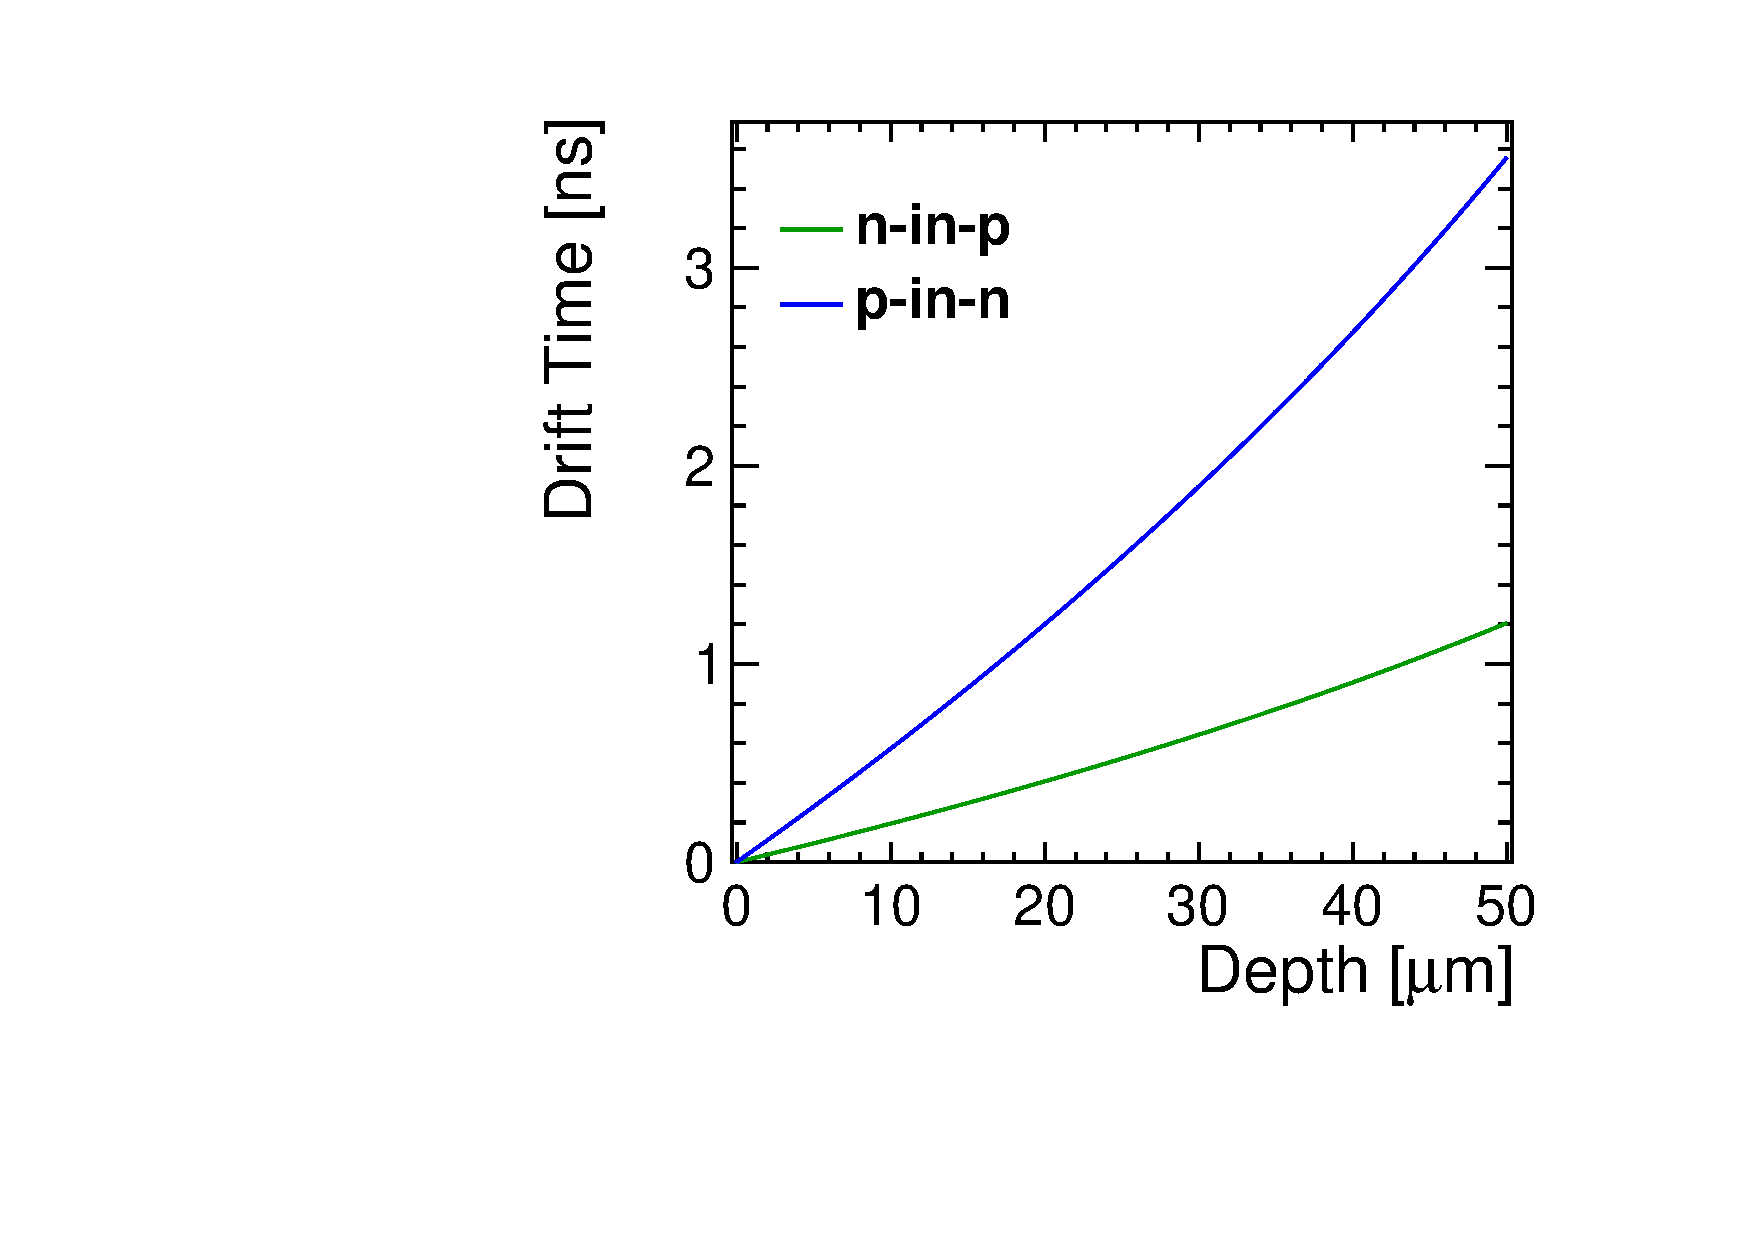
\includegraphics[width=\textwidth]{figures/ChargeSharing/DriftTime_n_vs_p_carrier.pdf}
    \caption{}
  \end{subfigure}\hfill
  \begin{subfigure}[b]{0.45\textwidth}
    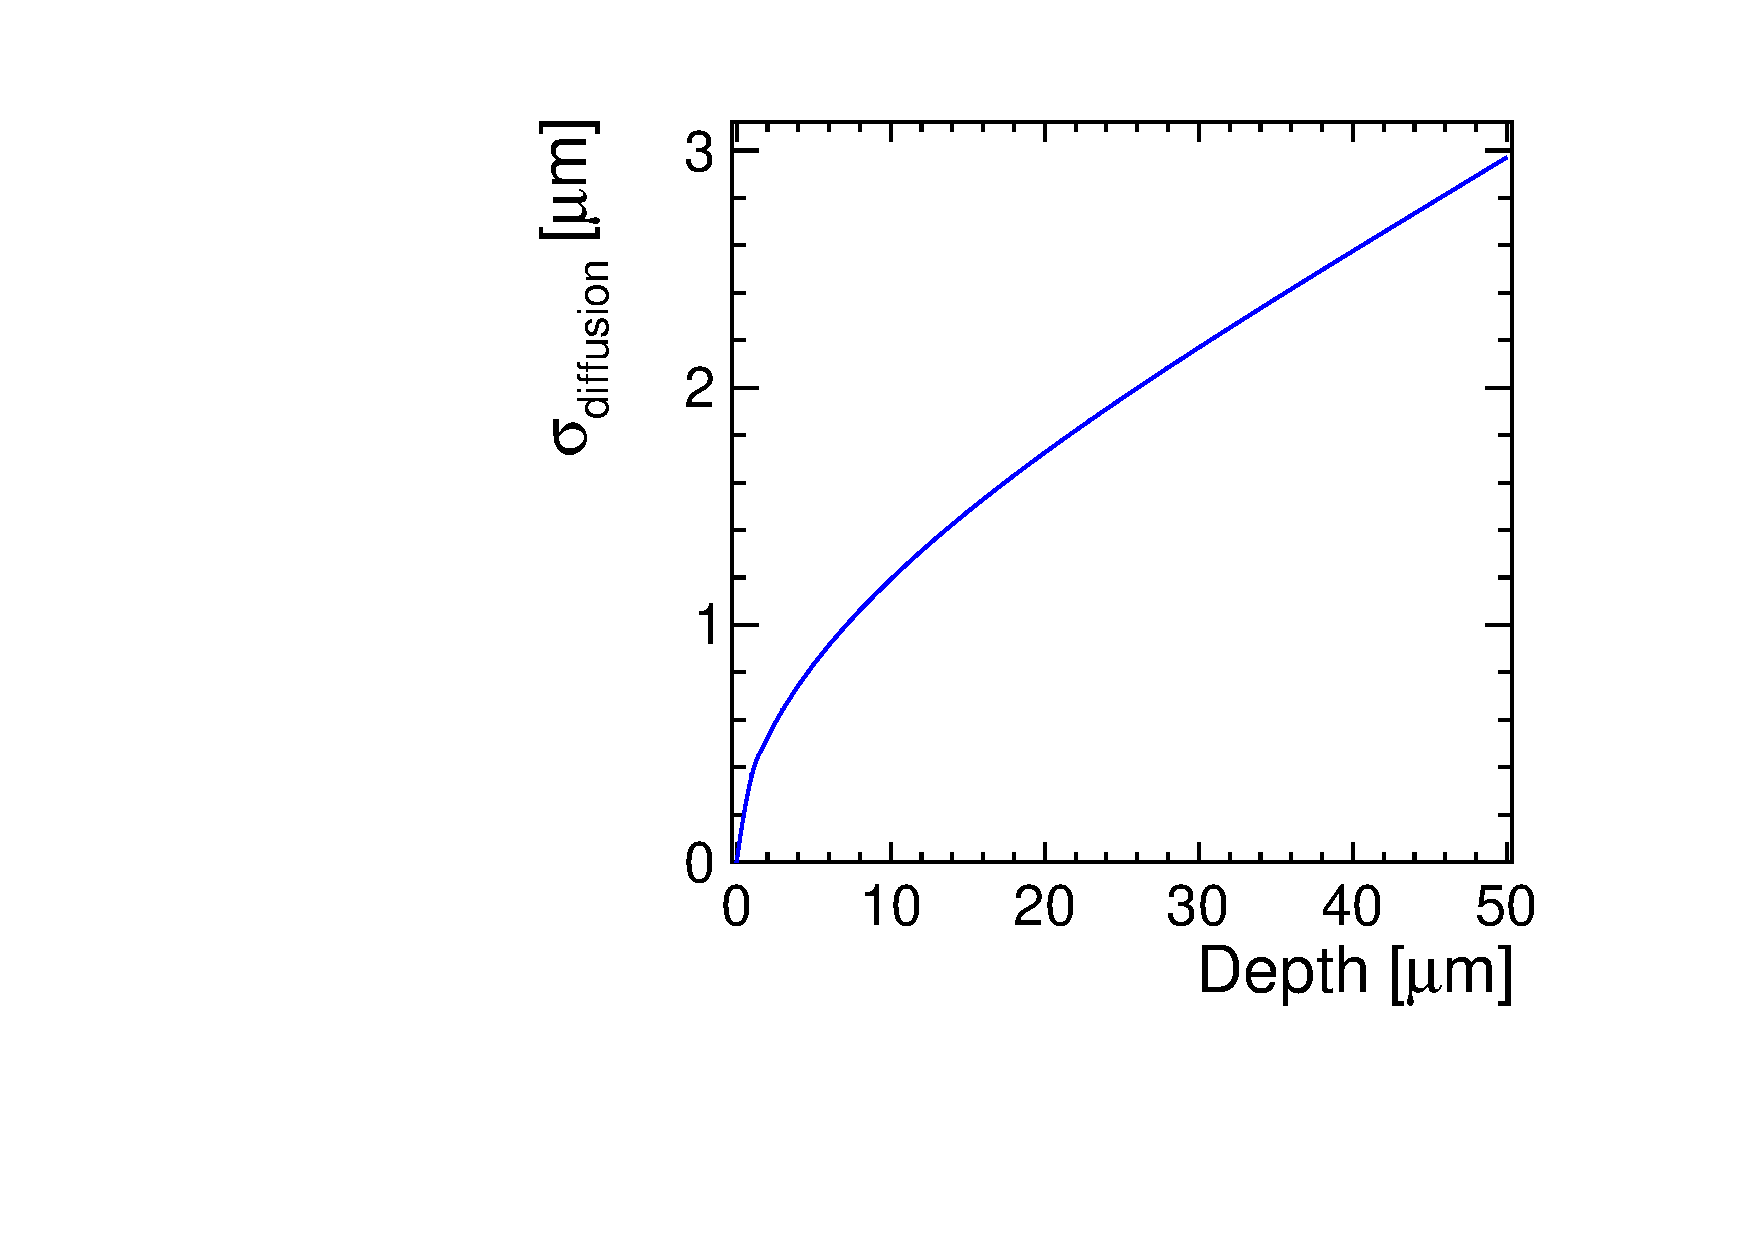
\includegraphics[width=\textwidth]{figures/ChargeSharing/Diffusion_n_vs_p_carrier.pdf}
    \caption{}
  \end{subfigure}
  \caption{(a) Drift time (b) diffusion standard deviation for n and
    p-type carriers as a function of the depth in the
    sensor. Diffusion does not depend on the carrier type. The
    depletion voltage is |V\textsubscript{D}|=4~V and the bias voltage
    is |V\textsubscript{B}|=15~V.}\label{fig:Drift_n_vs_p}
\end{figure}

\begin{figure}[htbp]
  \centering
  \begin{subfigure}[b]{0.45\textwidth}
    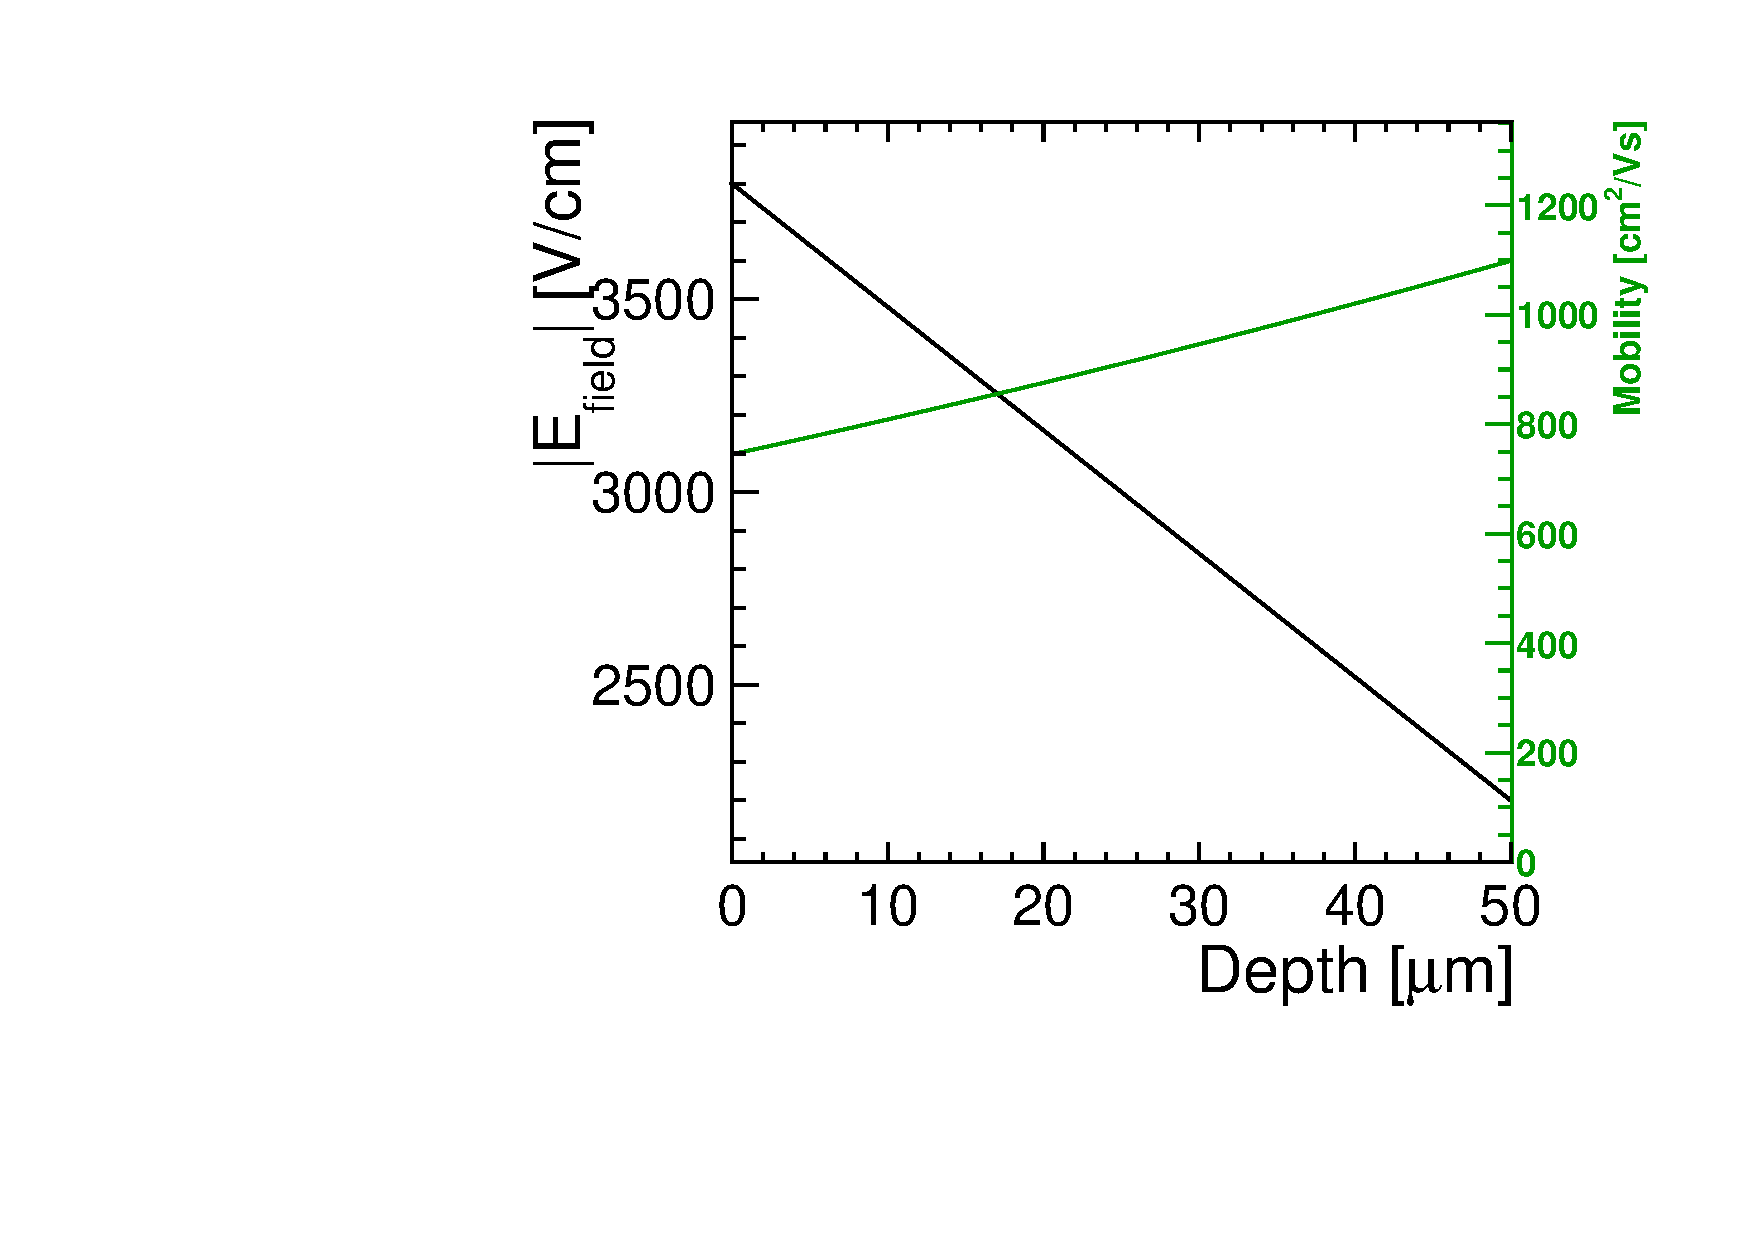
\includegraphics[width=\textwidth]{figures/ChargeSharing/Efield_mob_n_carrier.pdf}
    \caption{}
  \end{subfigure}\hfill
  \begin{subfigure}[b]{0.45\textwidth}
    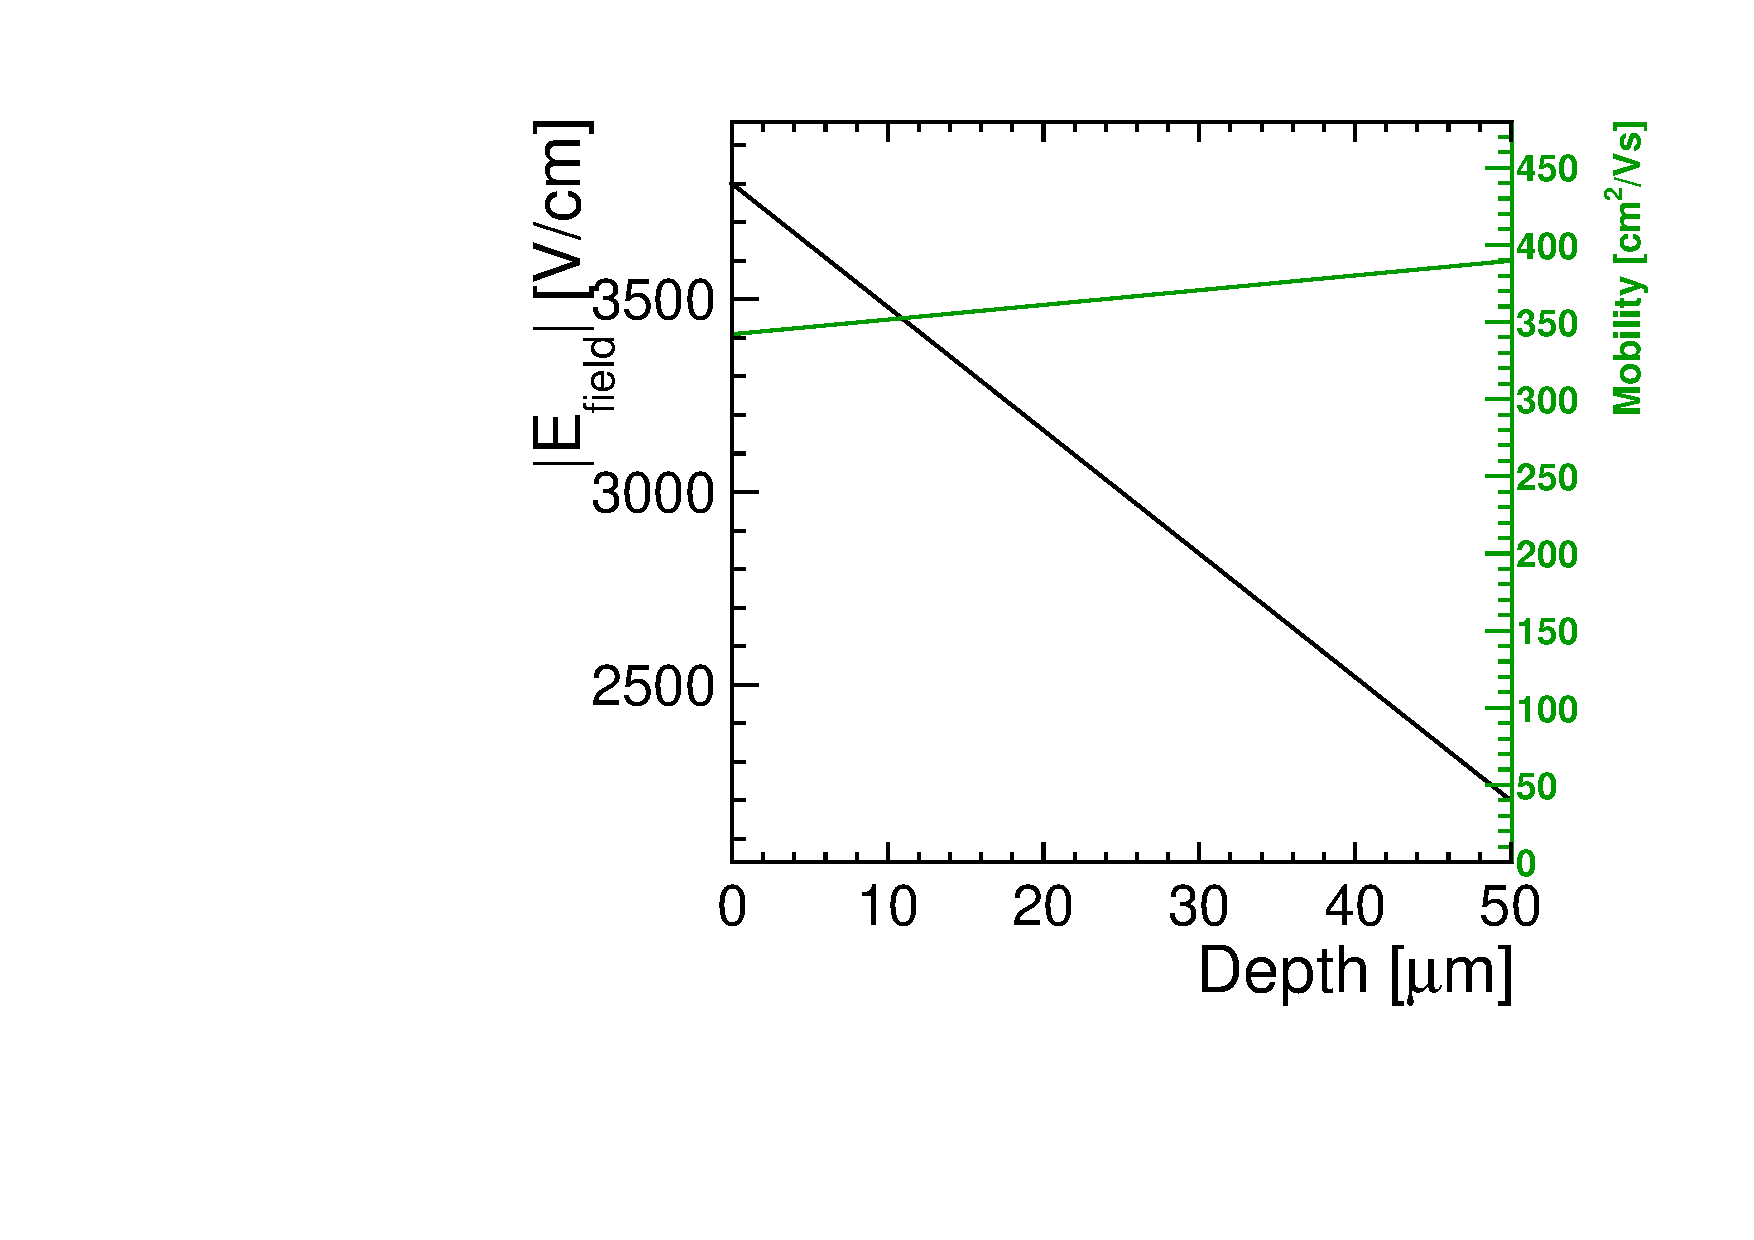
\includegraphics[width=\textwidth]{figures/ChargeSharing/Efield_mob_p_carrier.pdf}
    \caption{}
  \end{subfigure}
  \caption{The electric field and the mobility as a function of the
    depth for (a) n-type carriers and (b) p-type
    carriers.}\label{fig:Efield_n_vs_p}
\end{figure}

%% --------------------------------------------- %%
%% \subsection{TCAD simulations}

%%\newpage
\section{Pixelated silicon sensors properties}

Previously, we have reviewed the properties of a pn-junction as it is
the building block of pixel detectors. By segmenting the electrodes on
a pn-junction a pixel detector is obtained. The highly doped
electrodes, which can be n or p-type, are introduced through a mask to
form a pixel matrix with ion implantation. Each pixel forms an
independent pn-junction and the gaps between the pixels are
electrically controlled to isolate a pixel from its neighbouring
diodes. With an aluminum layer deposited on the electrodes provides
the external bias voltage and signal path to the readout electronics
with a low resistance.


%\subsection{Silicon sensors types}
%\subsection{Leakage current}
\subsection{Charge collection and Ramo's theorem: induced charge}
\label{sec:RamoTheorem}

Previously, we have seen that due to incident radiation, a signal is
produced by the motion of charge carriers in the detector. We can
naively interpret this statement as the signal is formed with a delay
when the charge carriers are collected by the electrodes. But in
reality, such a delay does not exist and a signal pulse is created
immediately after a charge carrier starts its motion to the
electrodes. When the last charge carriers arrive at the collecting
electrodes, the charge induction process ends and the signal pulse is
fully developed. The timing evolution of the signal is important in
understanding the timing properties of detectors. In the following, we
derive the induced charge in a pixel detector.

For the calculation of the induced charge, first, consider the simple
example of a charge $q$ near an infinitely large electrode with all
the electric field lines terminating on the electrode. The Gauss's
law, for a surface $S$ surrounding the charge is expressed as:

\begin{equation}
\oint_{s} \vec{E} \cdot d\vec{a}=q\; .
\label{eq:GaussLaw}
\end{equation}

The induced charge obtained by integrating over a Gaussian surface
enclosing only the electrode is $-q$. Considering two parallel
electrodes with a charge $q$ in between as showin in
\cref{fig:InducedCharge_parallelPlates}. If the charge is placed
midway between the two parallel plates, it induces equal charge of
$-q/2$ on the both electrodes as half of the electric field lines end
up on the higher and the other half on the lower electrode. When the
charge moves closer to a plate rather than the other, the induced
charge will be higher for the closer plate.

The induced charge can not be observed directly but its change can be
measured when the two electrodes are connected in a closed circuit
(like a pixel detector) as it produces an induced current.

\begin{figure}[htbp]
  \centering
  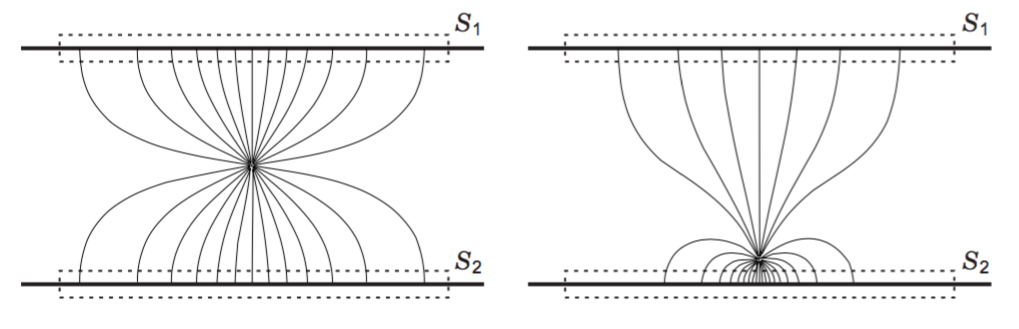
\includegraphics[width=0.8\textwidth]{figures/Ramo/InducedCharge_parallelPlates.png}
  \caption{The charge induced on two parallel plates depending on the
    position of the charge $q$. From~\cite{Spieler2005}.}
  \label{fig:InducedCharge_parallelPlates}
\end{figure}

Ramo's theorem~\cite{Ramo:1939vr} describes the time evolution of the
induced current created in a detector. The induced current on the
electrodes is described as a function of the weighting potential
$\Phi$ which describes the coupling of a charge to an electrode. The
weighting potential is defined for a specific electrode. In Ramo's
theorem, it is obtained by setting the potential of the electrode to 1
and setting all other electrodes to potential 0. \cref{eq:RamoCharge}
describes the induced charge $Q_k$ on electrode $k$ if a charge q
moves along any path from position $z_0$ to $z_p$:
\begin{equation}
    Q_{k}=q \cdot [\Phi_k(z_p)-\Phi_k(z_0)] \; .
   \label{eq:RamoCharge} 
  \end{equation}

It is important to note that the weighting potential (field) is
different than the electric potential (field). The electric field
determines the drift trajectory and velocity of the charge carriers
whereas the weighting field depends only on the geometry of the
electrodes and defines how the charge motion induces a charge to a
specific electrode. In the specific case of two-electrode
configuration the electric and the weighting fields are the same.


\cref{fig:RamoTCAD} shows the weighting field and potential
distributions calculated using TCAD simulations~\cite{synopsysTCAD}
(c.f. \cref{sec:TCAD}). For this study, we consider a silicon sensor
with 5 pixels, having a thickness of 200~\micron and over-depleted
with a bias voltage of \SI{50}{\volt} on the back-side. First,
\SI{0}{\volt} is applied to all the electrodes and then \SI{1}{\volt}
is applied to the electrode~$k$. By taking the difference between the
two configurations, the weighting potential and field are obtained.


\begin{figure}[htbp]
  \centering
  \begin{subfigure}[b]{0.49\textwidth}
    \centering
    \begin{tikzpicture}
      \node[anchor=south west,inner sep=0] (image) at (0,0){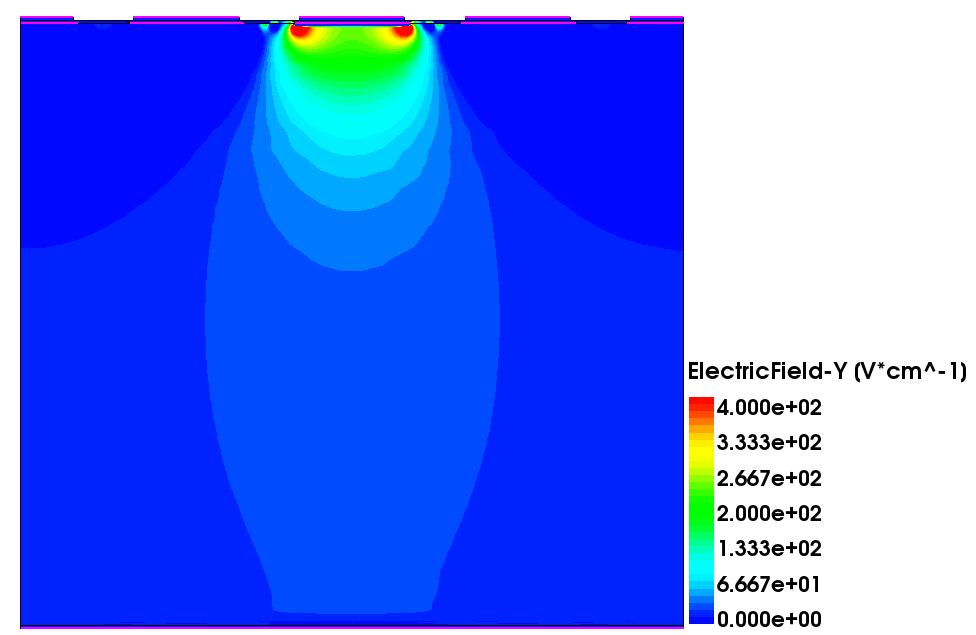
\includegraphics[width=\textwidth]{figures/Ramo/EfieldY_Ramo.png}};
      \begin{scope}[x={(image.south east)},y={(image.north west)}]
        \node[above, color=black] at (0.35, 1) {electrode $k$};
      \end{scope}
    \end{tikzpicture} 
    \caption{Weighting field}\label{fig:WeightingFieldRamo}
  \end{subfigure}\hfill
  \begin{subfigure}[b]{0.49\textwidth}
    \centering
    \begin{tikzpicture}
      \node[anchor=south west,inner sep=0] (image) at (0,0){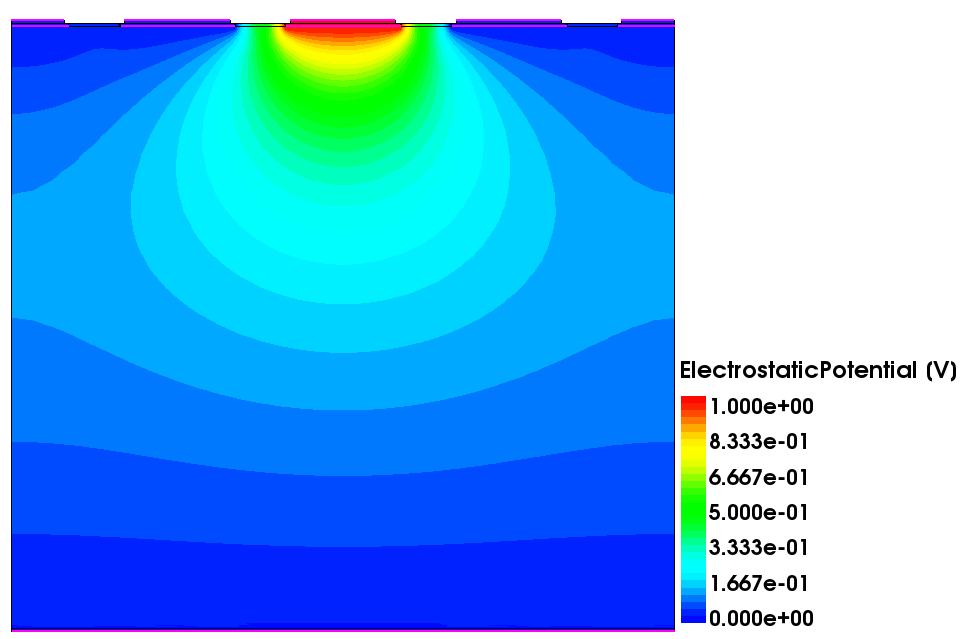
\includegraphics[width=\textwidth]{figures/Ramo/RamoPotential.png}};
      \begin{scope}[x={(image.south east)},y={(image.north west)}]
        \node[above, color=black] at (0.35, 1) {electrode $k$};
      \end{scope}
    \end{tikzpicture} 
    \caption{Weighting potential}\label{fig:WeightingPotentialRamo}
  \end{subfigure} 
  \caption{The weighting field and potential.}\label{fig:RamoTCAD}
\end{figure}

The weighting potential for different hit positions on the x-axis is
shown in \cref{fig:RamoTCADCuts}. Since, the total charge collected by
the electrode $k$ depends only on the depth positions $z_0$ and $z_p$,
in the absence of the radiation-induced damages (which would affect
the distributions of the electric and weighting fields), the Ramo
theorem can be neglected. The charge carriers drift following the
electric field distribution and the diffusion causes multi-pixel hits.

\begin{figure}[htbp]
  \centering
  \begin{subfigure}[b]{0.48\textwidth}
    \centering
    \begin{tikzpicture}
      \node[anchor=south west,inner sep=0] (image) at
      (0,0){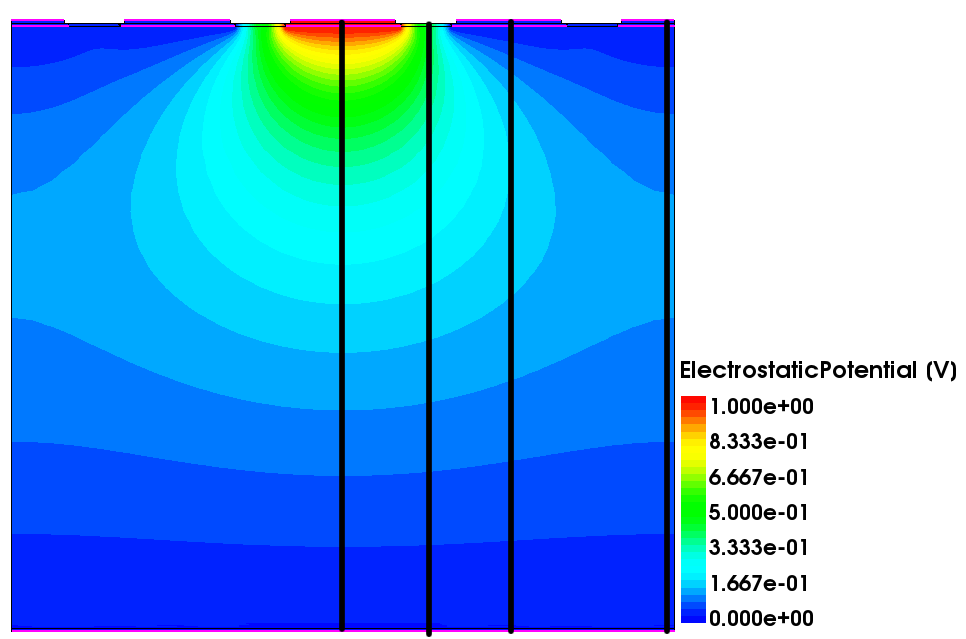
\includegraphics[width=\textwidth]{figures/Ramo/RamoPotential_cuts.png}};
      \begin{scope}[x={(image.south east)},y={(image.north west)}]
        \draw[->, thick] (-0.1, 1)--(0.73, 1) node[right]{$x$~$[\micron]$};
        \draw[->, thick] (0, 1.1)--(0, -0.1) node[below]{Depth $z$~$[\micron]$};
        \draw[-] (0.355, 1.01) -- (0.355, 0.99) node[above] {0};
        \draw[-] (0.445, 1.01) -- (0.445, 0.99) node[above] {27.5};
        \draw[-] (0.533, 1.01) -- (0.533, 0.99) node[above] {55};
        \draw[-] (0.69, 1.01) -- (0.69, 0.99) node[above] {109};


        \draw[-] (-0.01, 0.01) -- (0.01, 0.01) node[left] {200};
        \draw[-] (-0.01, 0.97) -- (0.01, 0.97) node[left] {0};
        %% \draw[help lines,xstep=.1,ystep=.1] (0, 0) grid (1,1);
        %% \foreach \x in {0,1,...,9} { \node [anchor=north] at (\x/10,0) {0.\x}; }
        %% \foreach \y in {0,1,...,9} { \node [anchor=east] at (0,\y/10) {0.\y}; }

      \end{scope}
    \end{tikzpicture} 
    \caption{}\label{fig:RamoPotentialCuts}
  \end{subfigure}\hfill
  \begin{subfigure}[b]{0.49\textwidth}
    \centering
    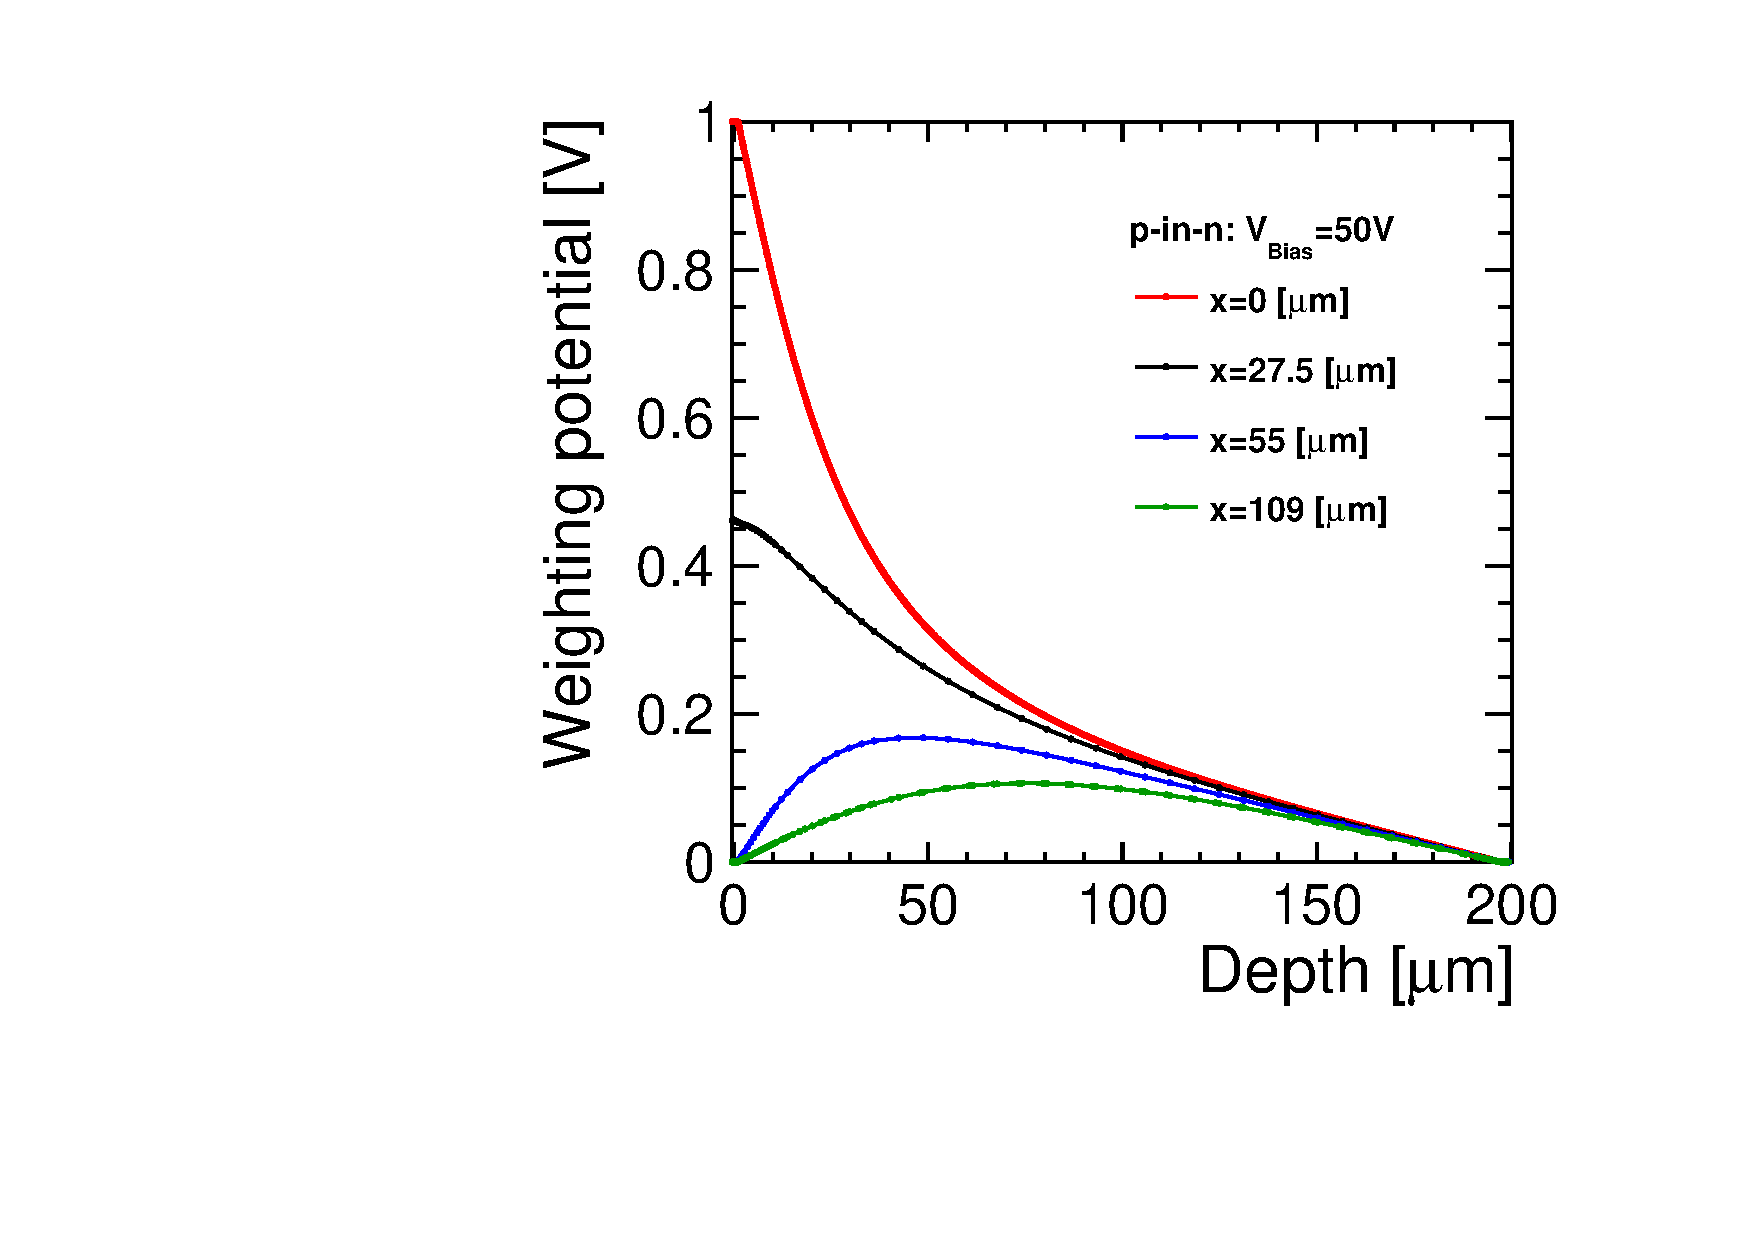
\includegraphics[width=0.9\textwidth]{figures/Ramo/WeightingPotential_1D.pdf}
    \caption{}\label{fig:RamoPotentialCuts1D}
  \end{subfigure} 
  \caption{The weighting potential for different positions on the x-axis using TCAD simulations. The detector has a thickness of $200\,\micron$.}
  \label{fig:RamoTCADCuts}
\end{figure}


\section{Spatial resolution}

The spatial resolution of a pixel detector is mainly determined by the
pixel pitch. But this can be improved by the readout choice (binary or
analogue), the threshold value, the charge sharing, thickness of the
detector and the reconstruction algorithm. The effect of the readout
is studied in the sections here-below.

The spatial resolution is defined by:
\begin{equation}
\sigma_{position}^2={{\int_{-p/2}^{p/2} \left(x_r-x_m\right)^2
    D\left(x_r\right) dx_r } \over { \int_{-p/2}^{p/2}
    D\left(x_r\right) dx_r }}\; ,
\label{eq:spatialRes}
\end{equation}

where $\sigma_{position}$ is the average distance between the real
impact position $x_r$ and the measured position $x_m$ of the particle
in a pixel. $D\left(x\right)$ is the hit probability density function
in a pixel. $p$ represents the pixel pitch size.

In the coming sections, the spatial resolution defined by
\cref{eq:spatialRes} is studied for different scenarios and
assumptions.

%% \begin{figure}[htbp]
%%   \centering
%%   \begin{subfigure}[b]{0.3\textwidth}
%%     \centering
%%     \begin{tikzpicture}
%%       \draw[->, thick] (-2,0)--(2,0) node[right]{$x$};
%%       \draw[->, thick] (0, -0.5)--(0, 2) node[above]{$D\left(x\right)$};
      
%%       \draw[-] (-1.5, 1) -- (-1.5, 0) node[below]{${-p \over 2}$};
%%       \draw[-] (-1.5, 1) -- (1.5, 1);
%%       \draw[-] (1.5, 1) -- (1.5, 0) node[below]{${p \over 2}$};
%%       \node[] at (0.2, 1.2) {1};
%%     \end{tikzpicture}
%%     \caption{}\label{fig:SpatResBinary}
%%   \end{subfigure}\hfill
%%   \begin{subfigure}[b]{0.3\textwidth}
%%     \centering
%%     \begin{tikzpicture}
%%       \draw[->, thick] (-2,0)--(2,0) node[right]{$x$};
%%       \draw[->, thick] (0, -0.5)--(0, 2) node[above]{$D\left(x\right)$};
      
%%       \draw[-] (-0.7, 1) -- (-0.7, 0) node[below]{\tiny ${{-(p-s)}\over 2}$};
%%       \draw[-] (-0.7, 1) -- (0.7, 1);
%%       \draw[-] (0.7, 1) -- (0.7, 0) node[below]{\tiny ${(p-s)\over 2}$};
%%       \node[] at (0.2, 1.2) {1};
%%       \draw[-] (-1.5, 0.1) -- (-1.5, 0) node[below] {${-p \over 2}$};
%%       \draw[-] (1.5, 0.1) -- (1.5, 0) node[below] {${p \over 2}$};
%%     \end{tikzpicture}
%%     \caption{}\label{fig:SpatResBinaryChargeSharing}
%%   \end{subfigure}\hfill
%%   \begin{subfigure}[b]{0.3\textwidth}
%%     \centering
%%     \begin{tikzpicture}
%%       \draw[->, thick] (-2,0)--(2,0) node[right]{$x$};
%%       \draw[->, thick] (0, -0.5)--(0, 2) node[above]{$D\left(x\right)$};
      
%%       \draw (-1.5,0) to[out=0, in=-120] (-0.9,0.2) to[out=60, in=180](-0.3, 1)--(0,1);
%%       \draw (0,1)--(0.3, 1) to [out=-20, in=120] (0.9,0.2) to[out=-60,
%%       in=0] (1.5,0);

%%       \draw[-] (-1.5, 0.1) -- (-1.5, 0) node[below] {${-p \over 2}$};
%%       \draw[-] (1.5, 0.1) -- (1.5, 0) node[below] {${p \over 2}$};

%%       \draw[-] (-0.5, 0.1) -- (-0.5, 0) node[below] {\tiny ${-(p-s) \over 2}$};
%%       \draw[-] (0.5, 0.1) -- (0.5, 0) node[below] {\tiny ${(p-s) \over 2}$};

%%       \node[] at (0.2, 1.2) {1};
%%     \end{tikzpicture}
%%     \caption{}\label{fig:SpatResAnaglogChargeSharing}
%%   \end{subfigure}
%%   \caption{(a) Binary readout. (b) Binary readout with charge
%%     sharing. (c) Analog readout with charge sharing.}\label{fig:SpatialResolution}
%% \end{figure}



\subsection{Binary readout} \label{sec:binaryReadout}
The simplest case for the resolution computation is to consider a
binary readout with single threshold for signal and noise
discrimination. For a pixel centered at 0 and having a pitch $p$ with
a probability density function as illustrated in
\cref{fig:SpatResBinary}, the following assumptions are considered:

\begin{itemize}
\item The threshold is adjusted in a way to fire one pixel per
  particle track.
\item Only hit positions between $-p/2$ and $p/2$ trigger a signal in
  pixel 0.
\item A uniform density of particles hit the detector ($D\left(x\right)=1$).
\end{itemize}


The average difference between the real position ($x_r$) and the
measured position ($x_m=0$) of the particle in a pixel is calculated
using \cref{eq:spatialRes} \cite{Rossi:976471}:
\begin{equation}
\sigma_{position}^2={{\int_{-p/2}^{p/2} \left(x_r\right)^2
    1 dx_r } \over { \int_{-p/2}^{p/2}
    1 dx_r }}={p^2 \over 12} \; ,
\label{eq:spatialResBinary}
\end{equation}
which results in a spatial resolution of:
\begin{equation}
\sigma_{position}={p \over \sqrt{12}} \;.
\label{eq:sigmaposBinary}
\end{equation}

\begin{figure}[htbp]
  \centering
  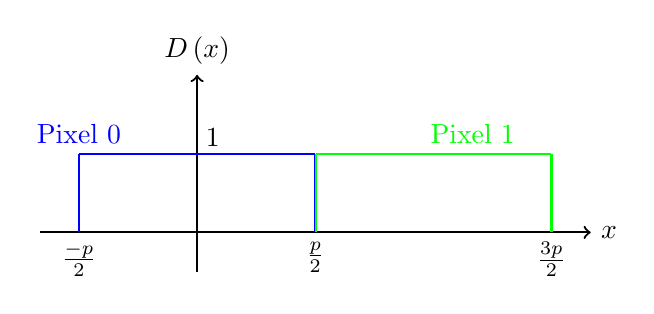
\begin{tikzpicture}
    \begin{scope}
      \draw[->, thick] (-2,0)--(5,0) node[right]{$x$};
      \draw[->, thick] (0, -0.5)--(0, 2) node[above]{$D\left(x\right)$};
      
      \draw[-, blue, thick] (-1.5, 1) -- (-1.5, 0);
      \node[below] at (-1.5, 0) {${-p \over 2}$};
      \draw[-, blue, thick] (-1.5, 1) -- (1.5, 1);
      \draw[-, blue, thick] (1.5, 1) -- (1.5, 0);
      \node[below] at (1.5, 0) {${p \over 2}$};
      \node[] at (0.2, 1.2) {1};
      \node[above, blue] at (-1.5, 1) {Pixel 0};

      \draw[-, green, thick] (1.51, 1) -- (1.51, 0);
      \draw[-, green, thick] (1.51, 1) -- (4.5, 1);
      \draw[-, green, thick] (4.5, 1) -- (4.5, 0);
      \node[below] at (4.5, 0) {${{3p} \over 2}$};
      \node[above, green] at (3.5, 1) {Pixel 1};
    \end{scope}
  \end{tikzpicture}
  \caption{The hit probability density function for two neighbouring
    pixels (pixel 0 and pixel 1) when a binary readout is used to
    acquire the sensor pulse.}
  \label{fig:SpatResBinary}
\end{figure}

This simple model shows the worst resolution achieved and is only
dependent on the pitch size (geometry of the pixels). In reality, with
charge sharing, the signal of a particle track is shared between
several pixels and depending on the readout threshold more than one
pixel can be fired which is called a \textit{cluster} of pixels. The
resolution is therefore improved as described in
\cref{sec:resolutionBinarySharing,sec:resolutionAnalogSharing}.

\subsection{Binary readout and charge sharing}\label{sec:resolutionBinarySharing}
The threshold of the readout electronics is usually set as low as
possible which can result in more than one pixel hit per particle
track. In this case, the charge is shared between two or more pixels
(called a cluster). Multi-hit clusters improve the resolution of
\cref{eq:sigmaposBinary}. \cref{fig:SpatResBinaryChargeSharing}
illustrates the charge sharing between two pixels. If a track passes
close to the edge of a pixel (within a distance of $s\over 2$ close to
the edge), then the neighbouring pixel is also fired. For events
triggering single-hit events, the spatial resolution in pixel 0 for
1-hit clusters is given by:

\begin{equation}
\sigma_{position}^2={{\int_{-(p/2-s/2)}^{(p/2-s/2)} \left(x_r\right)^2
    1 dx_r } \over { \int_{-(p/2-s/2)}^{(p/2-s/2)}
    1 dx_r }}={(p-s)^2 \over 12} \; .
\label{eq:spatialResCharge sharing_1hit}
\end{equation}

For two-hit clusters, the spatial resolution is given by:
\begin{equation}
\sigma_{position}={s \over \sqrt{12}} \; .
\label{eq:spatialResChargeSharing_2hit}
\end{equation}



\begin{figure}[htbp]
  \centering
  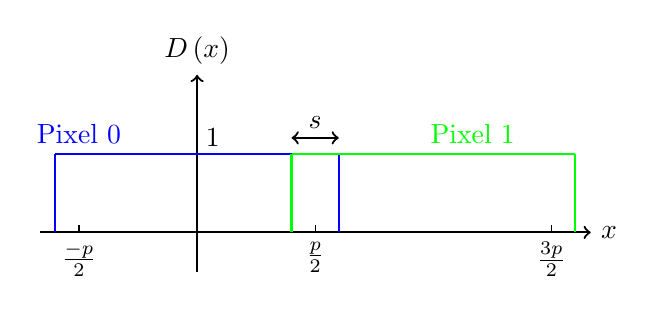
\begin{tikzpicture}
    \begin{scope}
      
      \draw[->, thick] (-2,0)--(5,0) node[right]{$x$};
      \draw[->, thick] (0, -0.5)--(0, 2) node[above]{$D\left(x\right)$};
      
      \draw[-, blue, thick] (-1.8, 1) -- (-1.8, 0);

      \draw[-] (-1.5, 0) -- (-1.5, 0.1);
      \node[below] at (-1.5, 0) {${-p \over 2}$};
      \draw[-, blue, thick] (-1.8, 1) -- (1.8, 1);
      \draw[-, blue, thick] (1.8, 1) -- (1.8, 0);

      \draw[-] (1.5, 0) -- (1.5, 0.1);
      \node[below] at (1.5, 0) {${p \over 2}$};
      \node[] at (0.2, 1.2) {1};
      \node[above, blue] at (-1.5, 1) {Pixel 0};
      
      \draw[-, green, thick] (1.2, 1) -- (1.2, 0);
      \draw[-, green, thick] (1.2, 1) -- (4.8, 1);
      \draw[-, green, thick] (4.8, 1) -- (4.8, 0);
      \draw[-] (4.5, 0) -- (4.5, 0.1);
      \node[below] at (4.5, 0) {${{3p} \over 2}$};
      \node[above, green] at (3.5, 1) {Pixel 1};

      \draw[<->, thick] (1.2, 1.2)--(1.8, 1.2);
      \node[above] at (1.5, 1.2) {$s$};
      
    \end{scope}
  \end{tikzpicture}
  \caption{The hit probability density function for two neighbouring
    pixels (pixel 0 and pixel 1) considering charge sharing between
    the two pixels when a binary readout is used to acquire the sensor
    pulse. For a track passing in the edge of the two pixels, within a
    distance of $s$/2 close to the edge, pixel 0 and pixel 1 are
    fired.}\label{fig:SpatResBinaryChargeSharing}
  % Binary readout with charge sharing.
\end{figure}

The average resolution considering single and multi-hit clusters is
given by:
\begin{equation}
{\sigma_{Total}^{2}}={{\left(p-s\right)^{2}} \over 12}+{{s^2}\over12} \; .
\label{eq:spatialResChargeSharingTotal}
\end{equation}

The optimal average spatial resolution is obtained for $s=p/2$ as
shown in \cref{fig:sigmaTotal} for two pixel pitches of is
$p=25\,\micron$ and $p=55\,\micron$. This means that the number of
single-hit and multi-hit clusters is the same. But, in this situation
one is not able to distinguish between one track triggering two pixels
and two tracks hitting the sensor within $2p$.

\begin{figure}[htbp] \centering
  \begin{subfigure}[b]{0.45\textwidth}
    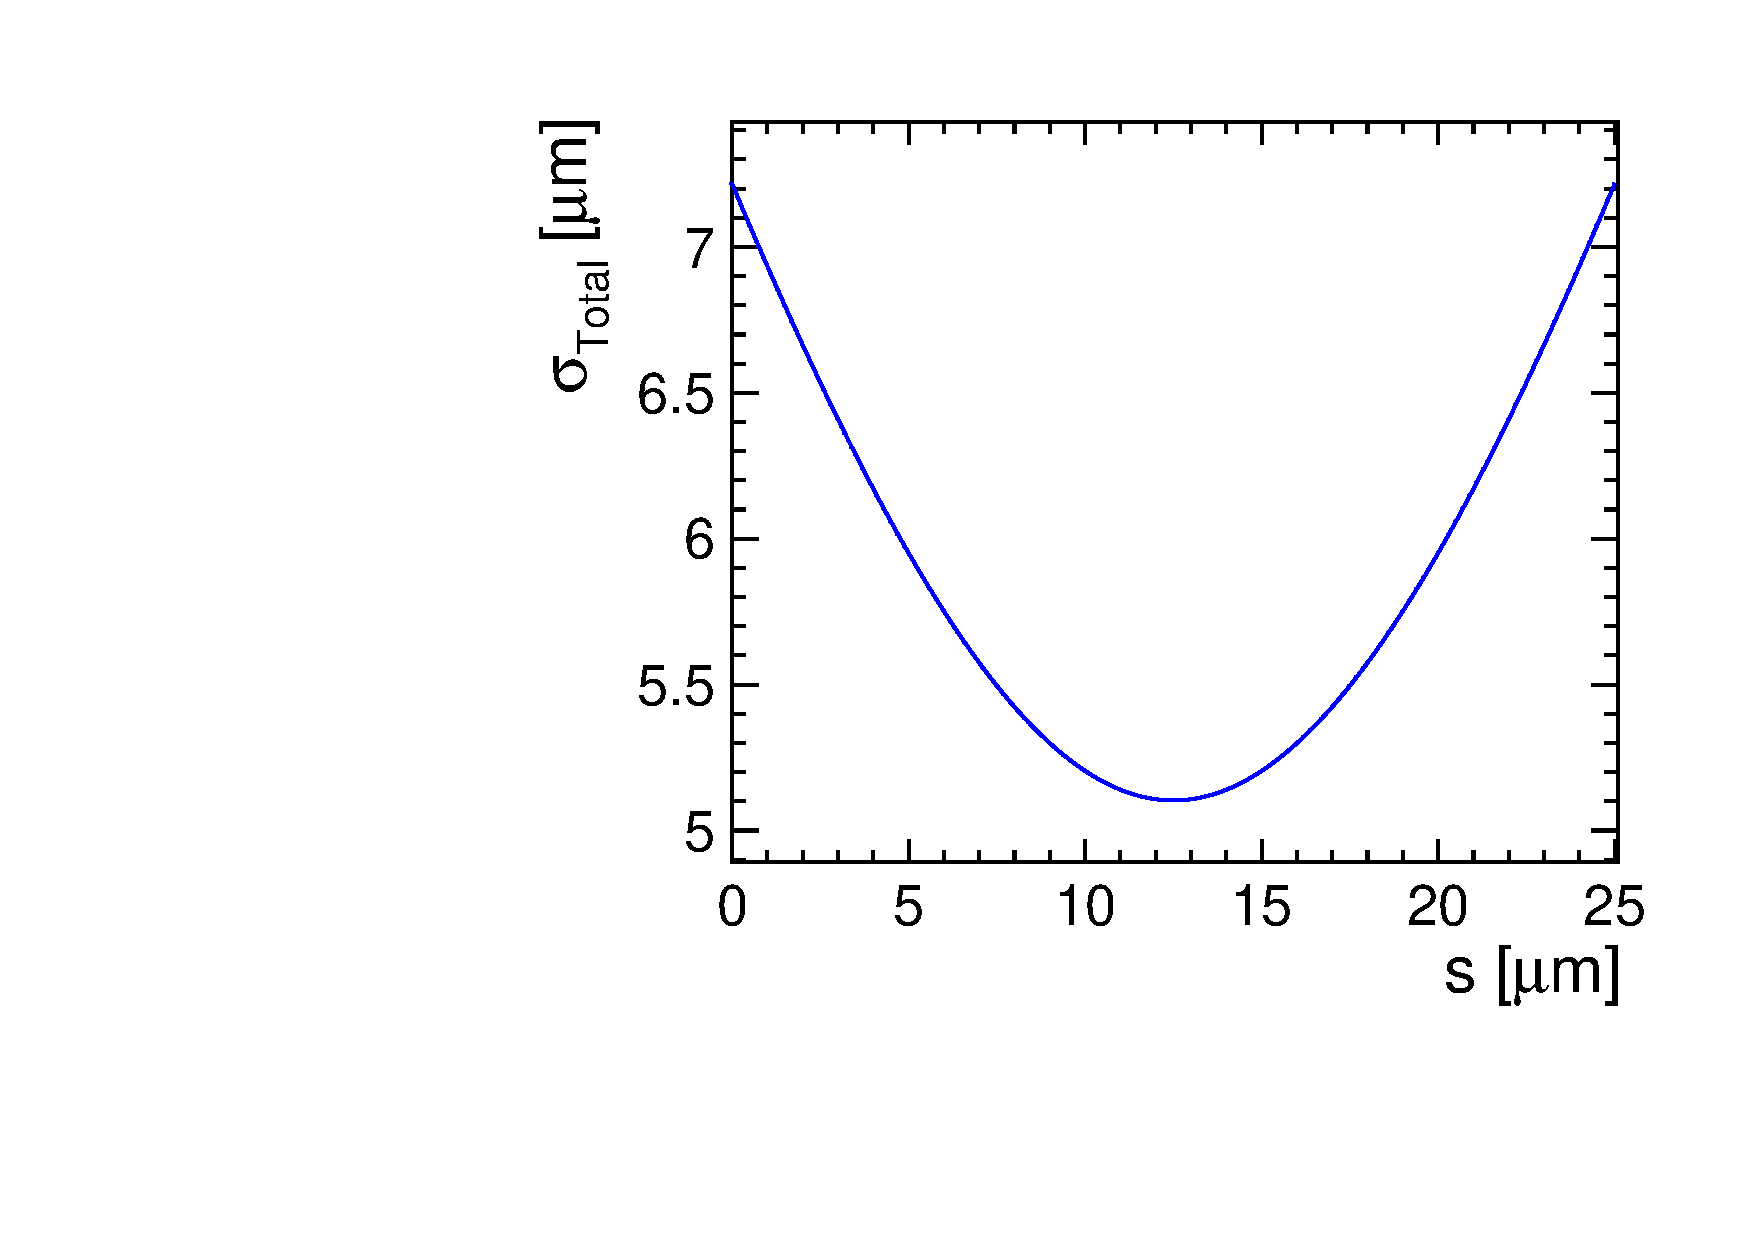
\includegraphics[width=\textwidth]{figures/ChargeSharing/resolution_binary_chargeSharing_s_25mupitch.pdf}
    \caption{$25\,\micron$ pitch}
  \end{subfigure} \hfill
  \begin{subfigure}[b]{0.45\textwidth}
    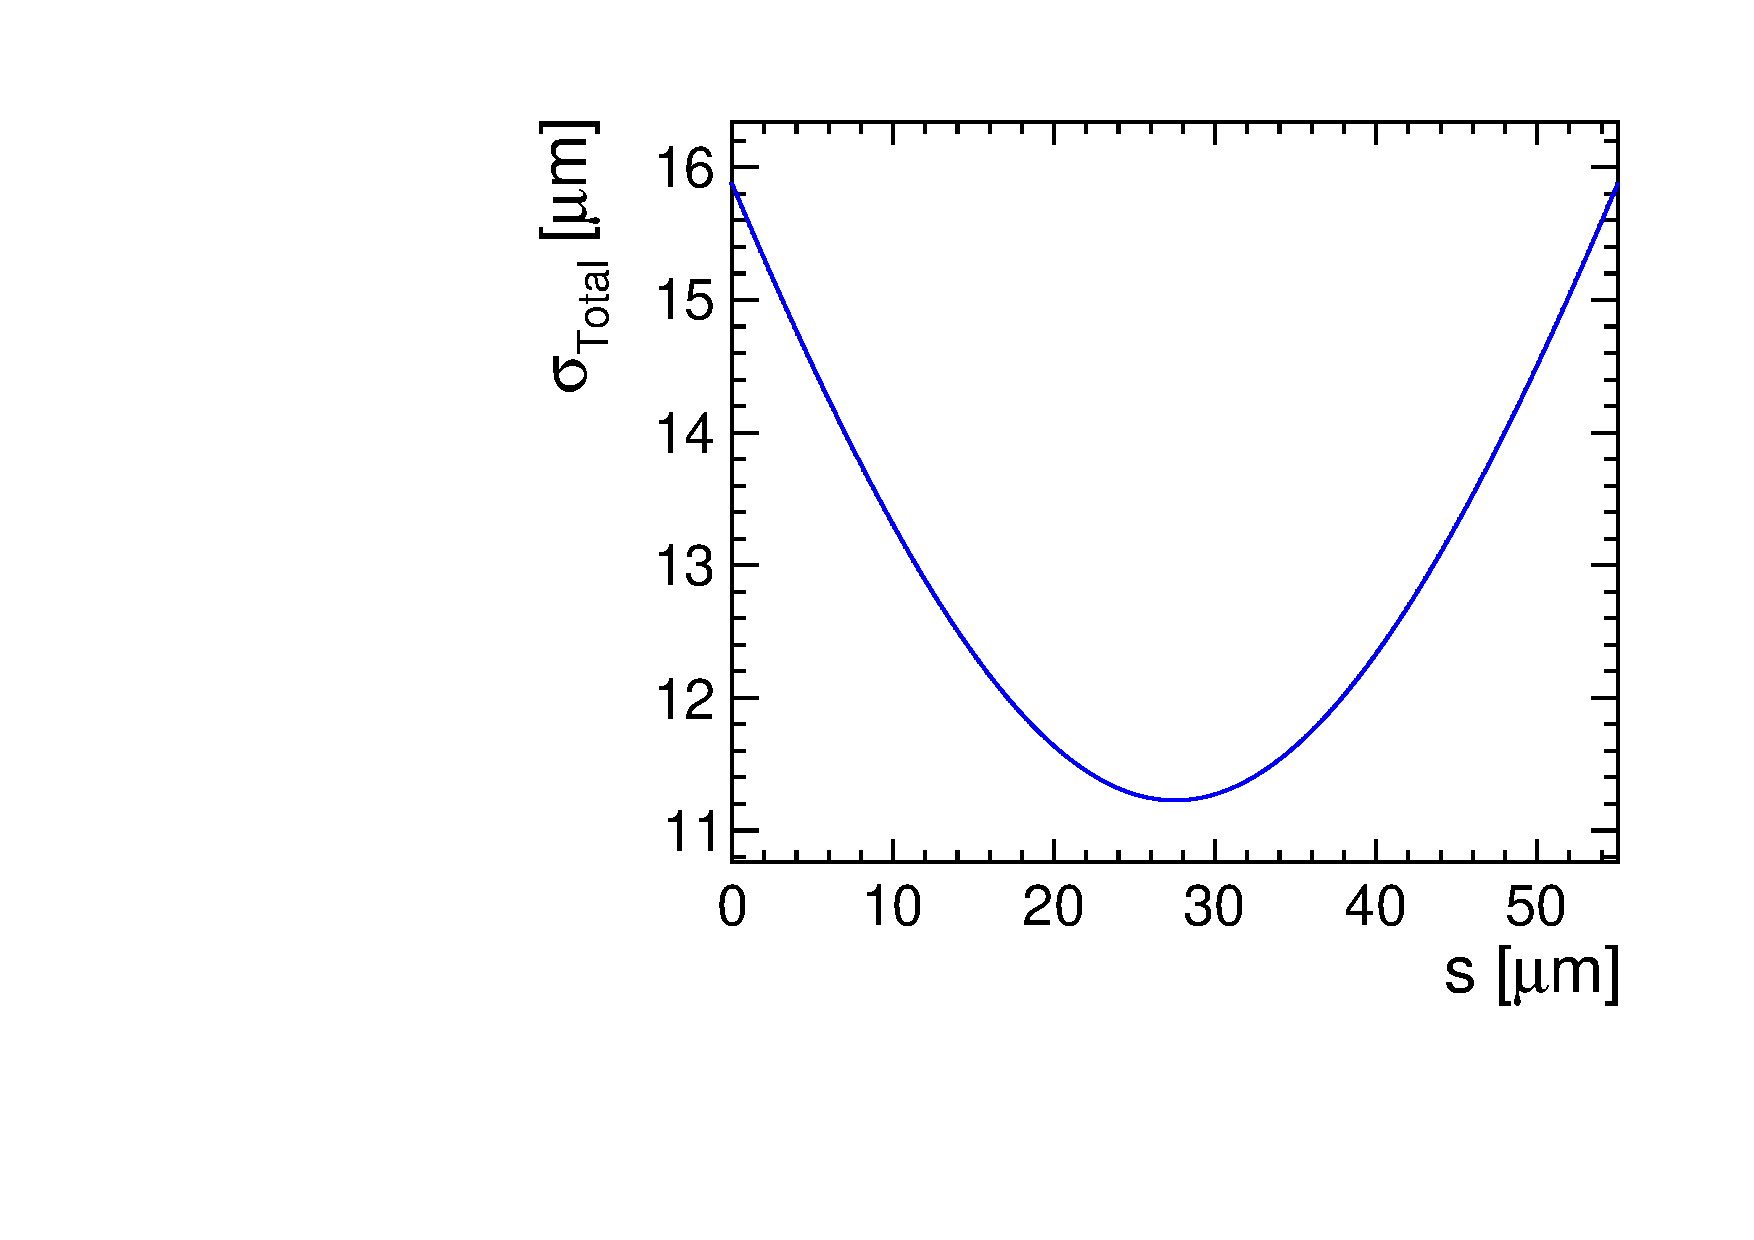
\includegraphics[width=\textwidth]{figures/ChargeSharing/resolution_binary_chargeSharing_s.pdf}
    \caption{$55\,\micron$ pitch}
  \end{subfigure}
  \caption{$\sigma_{\text{Total}}$ calculated using
    \cref{eq:spatialResChargeSharingTotal} with a pixel pitch of (a)
    $p=25\,\micron$ and (b) $p=55\,\micron$ where $s$ is the width of
    the charge sharing region as shown in
    \cref{fig:SpatResBinaryChargeSharing}.}
  \label{fig:sigmaTotal}
\end{figure}

%% --------------------------------------------------- %%
\subsection{Analogue readout and charge sharing}
\label{sec:resolutionAnalogSharing}
The spatial resolution can be significantly improved with an analogue
readout which delivers a signal proportional to the collected charge
as illustrated in \cref{fig:SpatResAnaglogChargeSharing}. In this
case, for multi-hit clusters the $\eta$-function~\cite{Belau:1983eh}
(c.f.~\cref{sec:EtaCorrection}) is used to reconstruct the hit
position within the pixels using the charge information. In the region
where only one pixel fires, the resolution is still limited to
$(p-s)\over \sqrt{12}$. In this case, the readout threshold is wished
to be as low as possible in order to detect the smallest amounts of
charge.

%% The charge carriers follow the field lines to end-up on a certain
%% electrode. They are also subject to thermal diffusion which spreads
%% the charge cloud as it drifts through the silicon. The width of the
%% diffusion $\sigma_{diffusion}(z)$ (for simplicity called $\sigma(z)$)
%% at depth $z$ is given by \cref{eq:driftTimeIntegrated}. The charge
%% distribution at position $x_{hit}$ for a pixel extending from $x_1$ to
%% $x_2$ is:
%% \begin{equation}
%% Q(x_{hit}, z)= Q(z) {1\over{\sqrt{2 \pi \sigma^2(z)}}}
%% {\int_{x_1}^{x_2} e^{-({{x-x_{hit}}\over{\sqrt{2} \sigma(z)}})^2} } dx\; .
%% \label{eq:ChargeDistribution}
%% \end{equation}

%% By integrating \cref{eq:ChargeDistribution} over the whole
%% thickness of the detector, the charge deposited in a pixel at
%% coordinate $x_{hit}$ having coordinates $x_1$ and $x_2$ is given by:  
%% \begin{equation}
%% Q(x_{hit})= \int_{x_1}^{x_2}  \int_{0}^{d} {Q(z) \over {\sqrt{2 \pi
%%       \sigma^2(z)}} } e^{-({{x-x_{hit}}\over{\sqrt{2} \sigma(z)}})^2}
%%   dz \; dx\; .
%% \label{eq:ChargeDistribution_integrated_z}
%% \end{equation}


\begin{figure}[htbp]
  \centering
  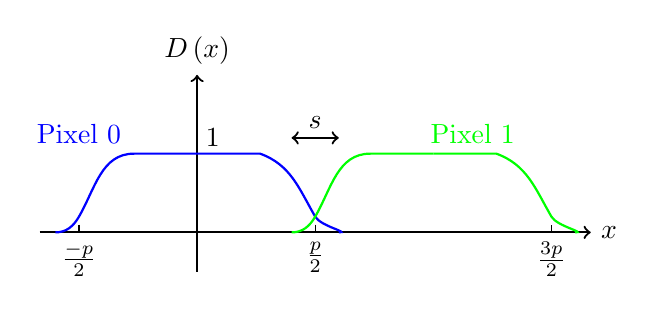
\begin{tikzpicture}
    \begin{scope}
      
      \draw[->, thick] (-2,0)--(5,0) node[right]{$x$};
      \draw[->, thick] (0, -0.5)--(0, 2) node[above]{$D\left(x\right)$};
      
      \draw[thick, blue] (-1.8,0) to[out=0, in=-120] (-1.5,0.2) to[out=60, in=180](-0.8, 1)--(0,1);
      \draw[thick, blue] (0,1)--(0.8, 1) to [out=-20, in=120] (1.5, 0.2) to[out=-60, in=0] (1.8,0);

      \draw[-] (-1.5, 0.1) -- (-1.5, 0) node[below] {${-p \over 2}$};
      \draw[-] (1.5, 0.1) -- (1.5, 0) node[below] {${p \over 2}$};
      \node[above, blue] at (-1.5, 1) {Pixel 0};

      \node[] at (0.2, 1.2) {1};


      \draw[thick, green] (1.2,0) to[out=0, in=-120] (1.5,0.2) to[out=60, in=180](2.2, 1)--(3,1);
      \draw[thick, green] (3,1)--(3.8, 1) to [out=-20, in=120] (4.5, 0.2) to[out=-60, in=0] (4.8,0);
      \draw[-] (4.5, 0) -- (4.5, 0.1);
      \node[below] at (4.5, 0) {${{3p} \over 2}$};
      \node[above, green] at (3.5, 1) {Pixel 1};

      \draw[<->, thick] (1.2, 1.2)--(1.8, 1.2);
      \node[above] at (1.5, 1.2) {$s$}; 
    \end{scope}
  \end{tikzpicture}
  \caption{The hit probability density function for two neighbouring
    pixels (pixel 0 and pixel 1) considering charge sharing between
    the two pixels using an analogue to acquire the sensor
    pulse.}\label{fig:SpatResAnaglogChargeSharing}
\end{figure}

%% --------------------------------------------------- %%
\section{The $\eta$-correction method}
\label{sec:EtaCorrection}

Due to the charge sharing, particle tracks create multi-pixel
clusters. The hit position within the pixel is reconstructed by using
the charges of the hit pixels as weights. This also takes into account
non-linearities in the charge sharing between
pixels~\cite{Belau:1983eh}.

The $\eta$-correction method calculates the distance with which the
hit position moves from the geometric centre of two pixels in a
cluster.

\begin{equation}
  \text{shift}=\sigma_{EC} \times \text{erf}^{-1}(2\times Q_{rel}-1) \; ,
  \label{eq:EtaCorrectionShift}
\end{equation}

where $\sigma_{EC}$ is a parameter to be determined and depends on
several factors such as the thickness of the silicon sensor, the
operating conditions of the assembly. The inverse error function
defined as erf\textsuperscript{-1} (z) where:

\begin{equation}
\text{erf(z)}={2\over\sqrt{\pi}} \int_{0}^{z} e^{-t^2} dt \; .
  \label{eq:EtaCorrectionErf}
\end{equation}

In \cref{eq:EtaCorrectionShift}, $Q_{rel}$ is the maximum charge of
the cluster divided by the total charge of the cluster
($Q_{max}/Q_{rel}$).


%% --------- Recycle text --------- %%
% \section{Detector systems}

% Figure~\ref{fig:basicDetectorFunction}, schematically summarises the sequence of basic detector functions.


% \begin{figure}[htbp]
%   \centering
%   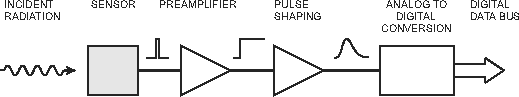
\includegraphics[width=\textwidth]{figures/basicDetectorFunction.png}
%   \caption{The sequence of basic detector functions. From~\cite{Spieler2005}.}
%   \label{fig:basicDetectorFunction}
% \end{figure}


% \subsection{Sensor} 
% A silicon sensor, converts the energy deposited by a particle to an electric signal by producing electron-hole pairs. By applying an electric field to the sensor, the produced pairs are con
% \subsection{Preamplifier}
% \subsection{Pulse shaper}
% \subsection{Digitiser}

%% --------------------------------------------------- %%
% Carriers move in random direction due to the thermal energy. \\
% Material-dependent diffusion constant given by the Einstein equation:  

% \begin{equation}
%   D_{b}={{k_{B} \cdot T \cdot \mu_{c}} \over {e}}
% \end{equation}
% where \(k=8.617 3324\) is the Boltzman constant.

% \begin{equation}
%   \sigma_{diffusion}=\sqrt{2 \cdot D_{b} \cdot t_{c}}
% \end{equation}






%% \begin{table}[htpb]
%%   \centering
%%   \caption{Sensors characteristics:}
%%   \label{tab:Efield_mobility}
%%   \begin{tabular}{ c c c c c c }
%%     \toprule
%%     Assembly & Sensor type & Thickness & V\textsubscript{depletion} &  V\textsubscript{bias} & THL\textsubscript{op} \\
%%     \midrule
%%     A06-W0110 & p-in-n & 50~\micron & $<15$~V & 15~V & 326 (855e\textsuperscript{-}) \\
%%     L04-W0125 & p-in-n & 100~\micron & 19.64~V & 35~V & 410 (916e\textsuperscript{-}) \\
%%     B06-W0125 & n-in-p & 200~\micron  & 30.31~V & -50~V & 435 (1066e\textsuperscript{-}) \\
%%     \bottomrule
%%   \end{tabular}
%% \end{table}

%% \begin{figure}[htbp]
%%   \centering
%%   \begin{subfigure}[b]{0.33\textwidth}
%%     \centering
%%     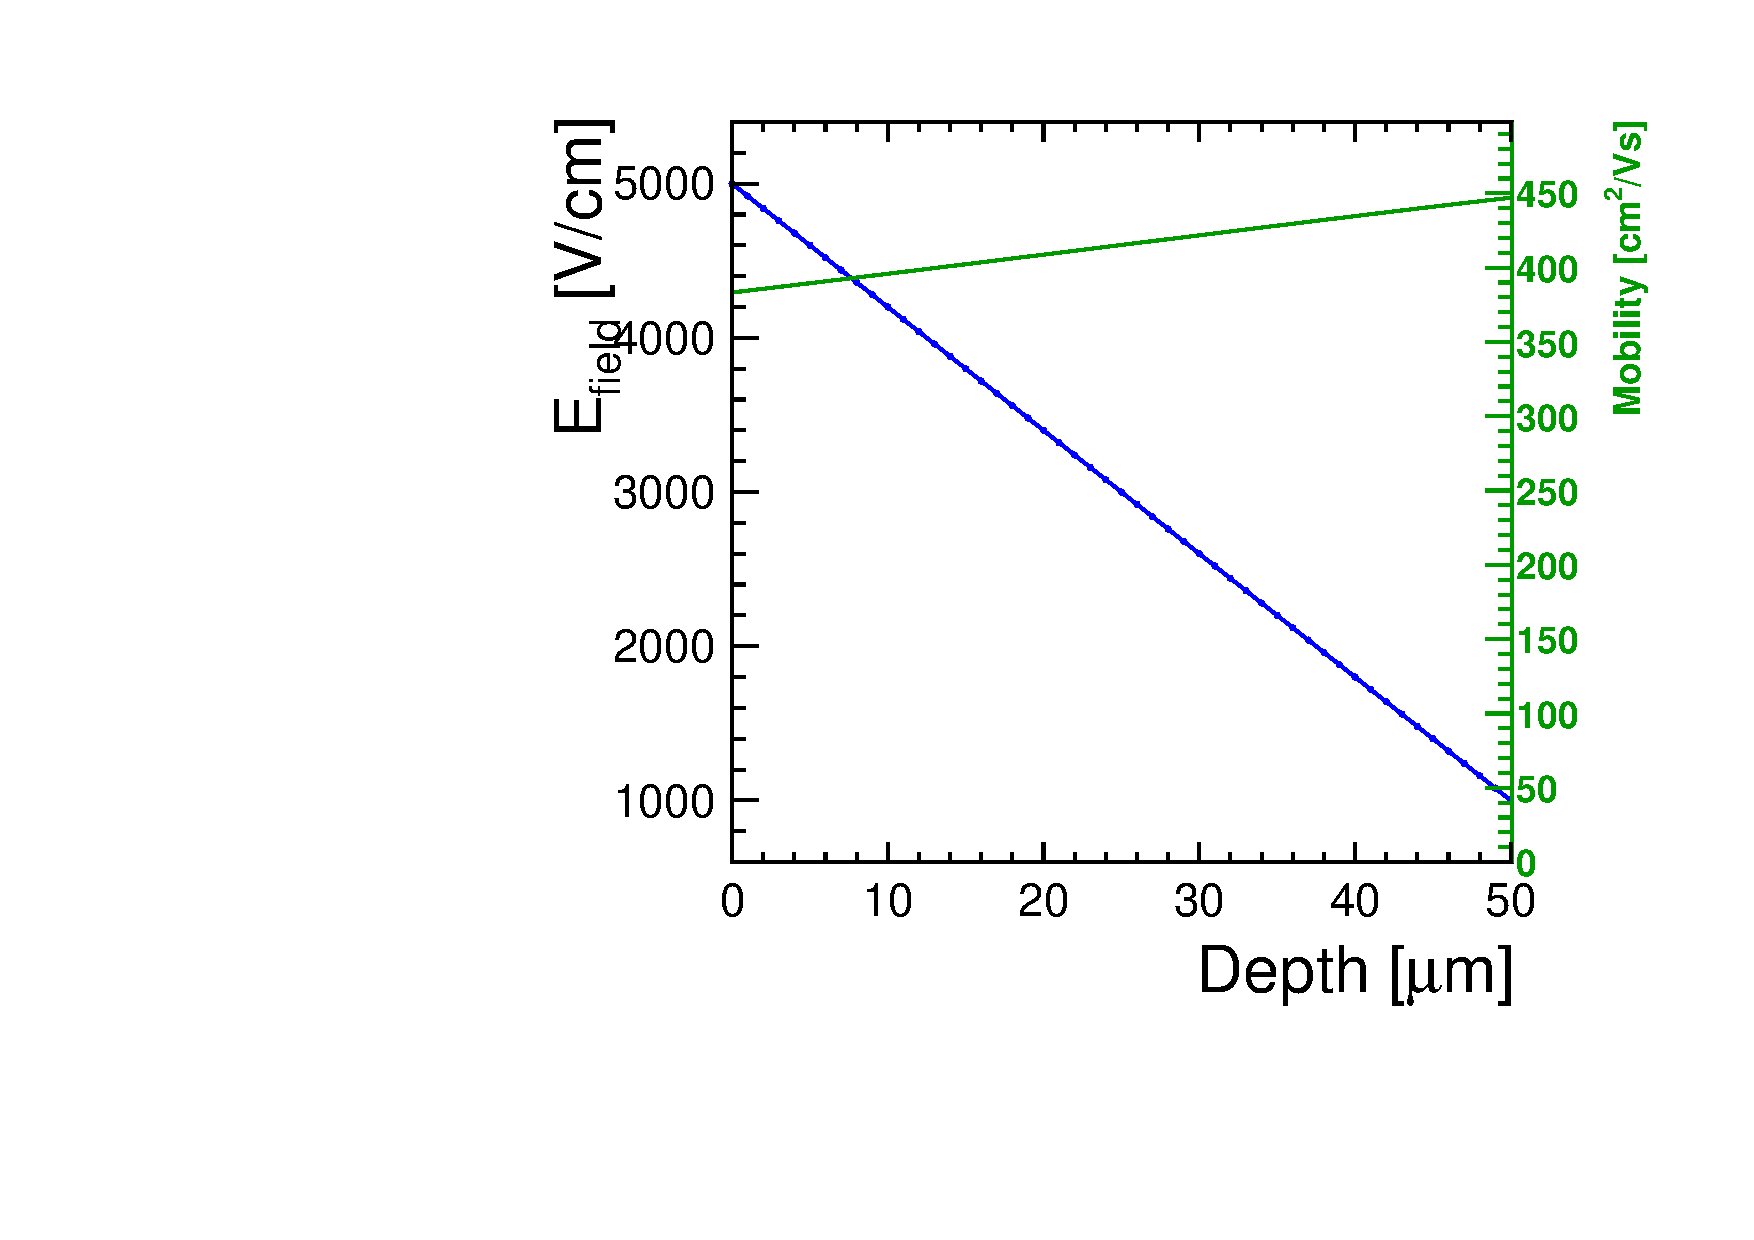
\includegraphics[width=\textwidth]{figures/ChargeSharing/Efield_mob_A06.pdf}
%%     \caption{50~\micron silicon}\label{fig:Mob_Efield_A06}
%%   \end{subfigure}\hfill
%%   \begin{subfigure}[b]{0.33\textwidth}
%%     \centering
%%     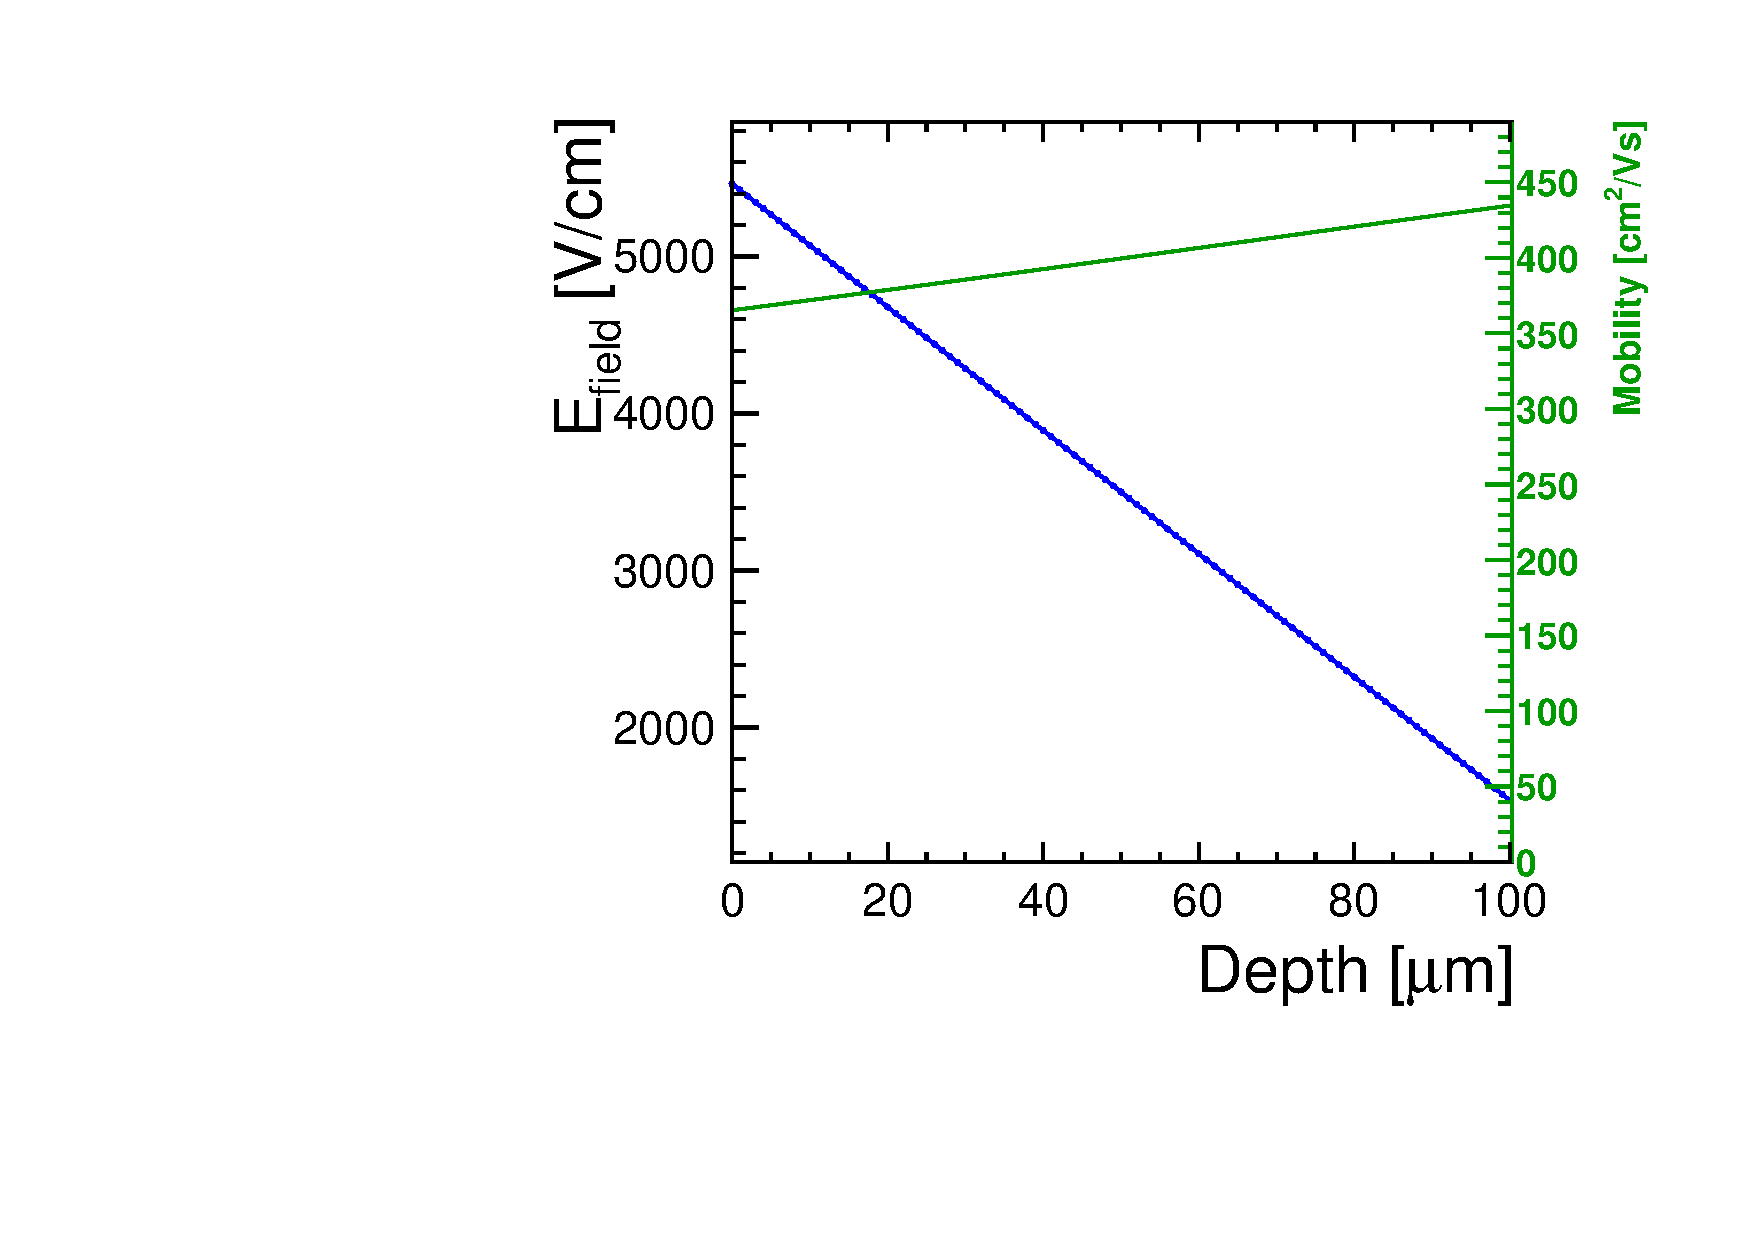
\includegraphics[width=\textwidth]{figures/ChargeSharing/Efield_mob_L04.pdf}
%%     \caption{100~\micron Silicon}\label{fig:Mob_Efield_L04}
%%   \end{subfigure} \hfill
%%   \begin{subfigure}[b]{0.33\textwidth}
%%     \centering
%%     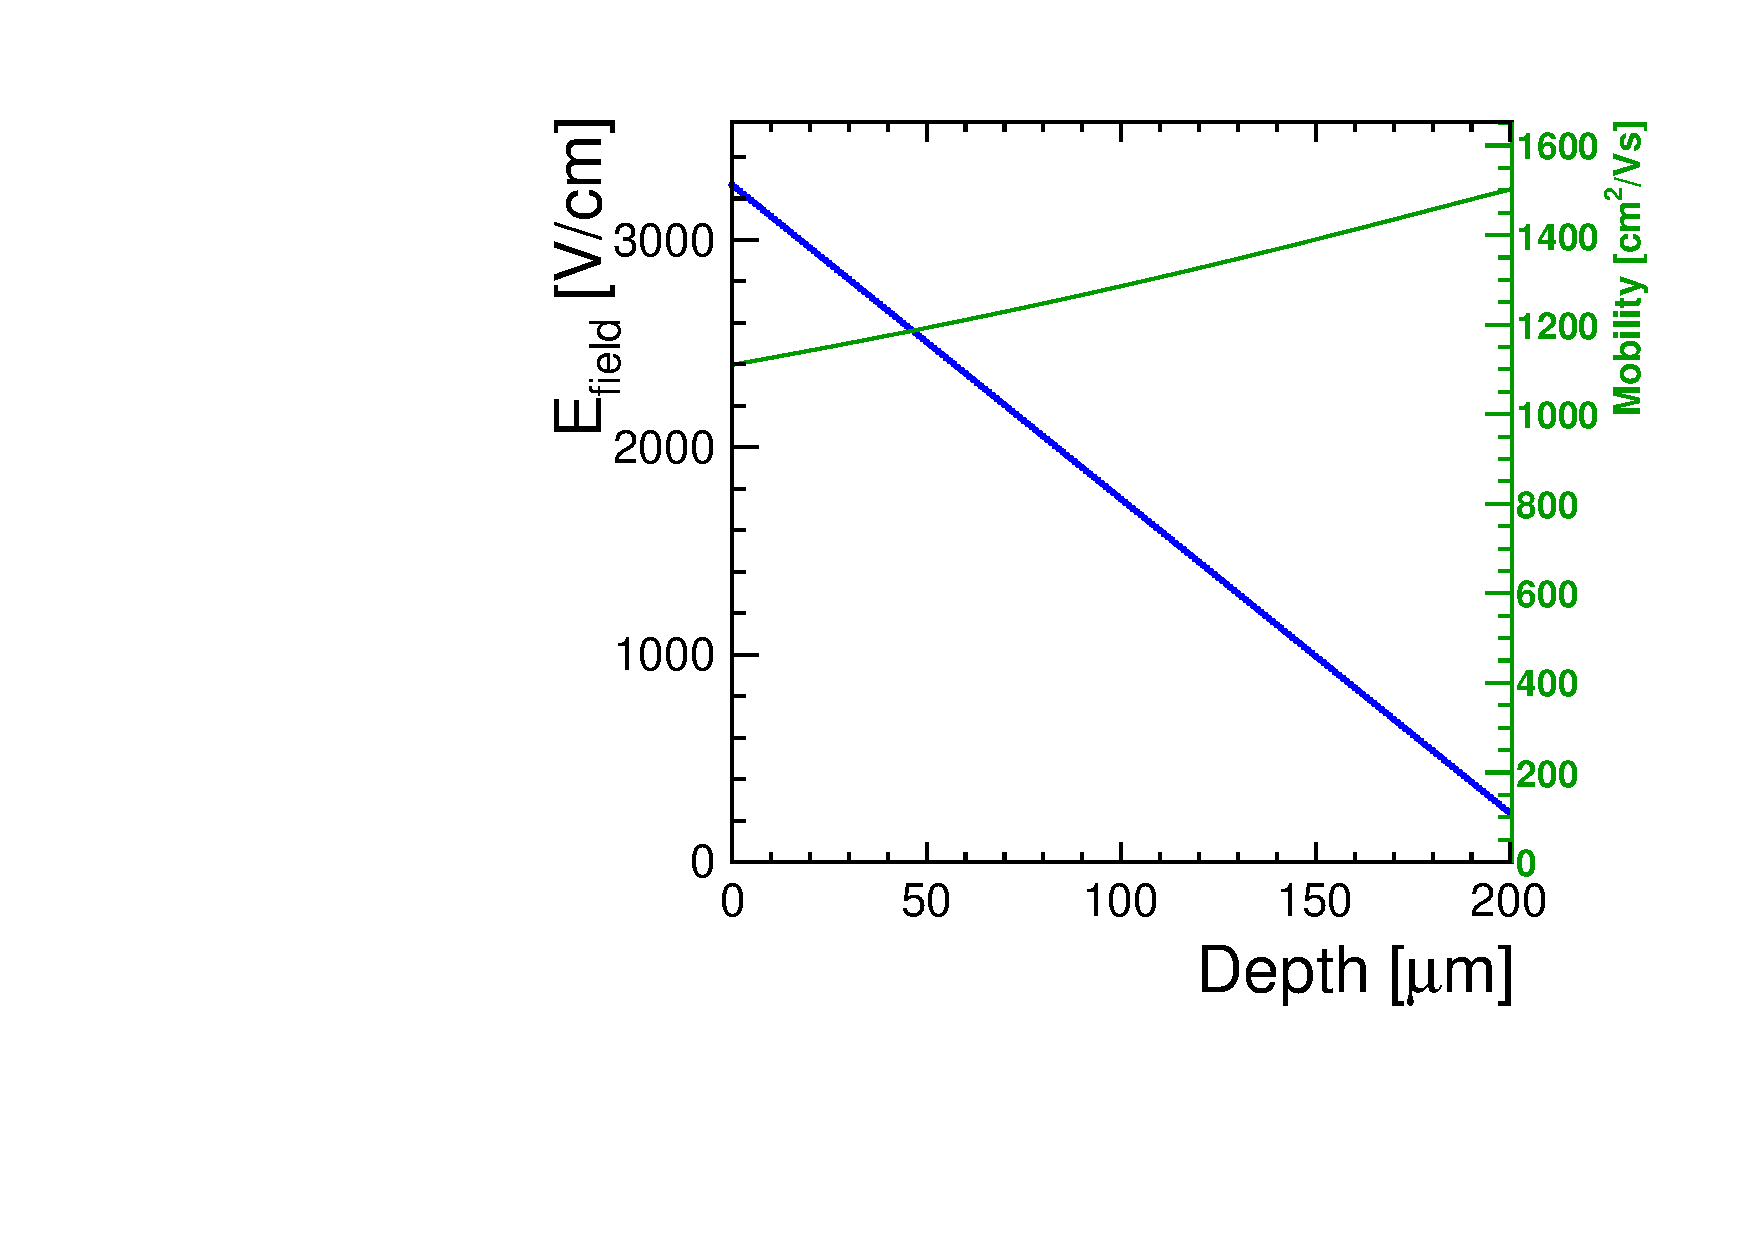
\includegraphics[width=\textwidth]{figures/ChargeSharing/Efield_mob_B06.pdf}
%%     \caption{200~\micron Silicon}\label{fig:Mob_Efield_B06}
%%   \end{subfigure} 
%%   \caption{Mobility dependence on the electric field.}\label{fig:Efield_mobility}
%% \end{figure}

%% Assuming the mobility constant is a good approximation for calculating
%% the charge sharing spread since the electric field is low. An example
%% is given for the case where the silicon sensor has a thickness of 200~\micron.

%% \begin{figure}[htbp]
%%   \centering
%%   \begin{subfigure}[b]{0.49\textwidth}
%%     \centering
%%     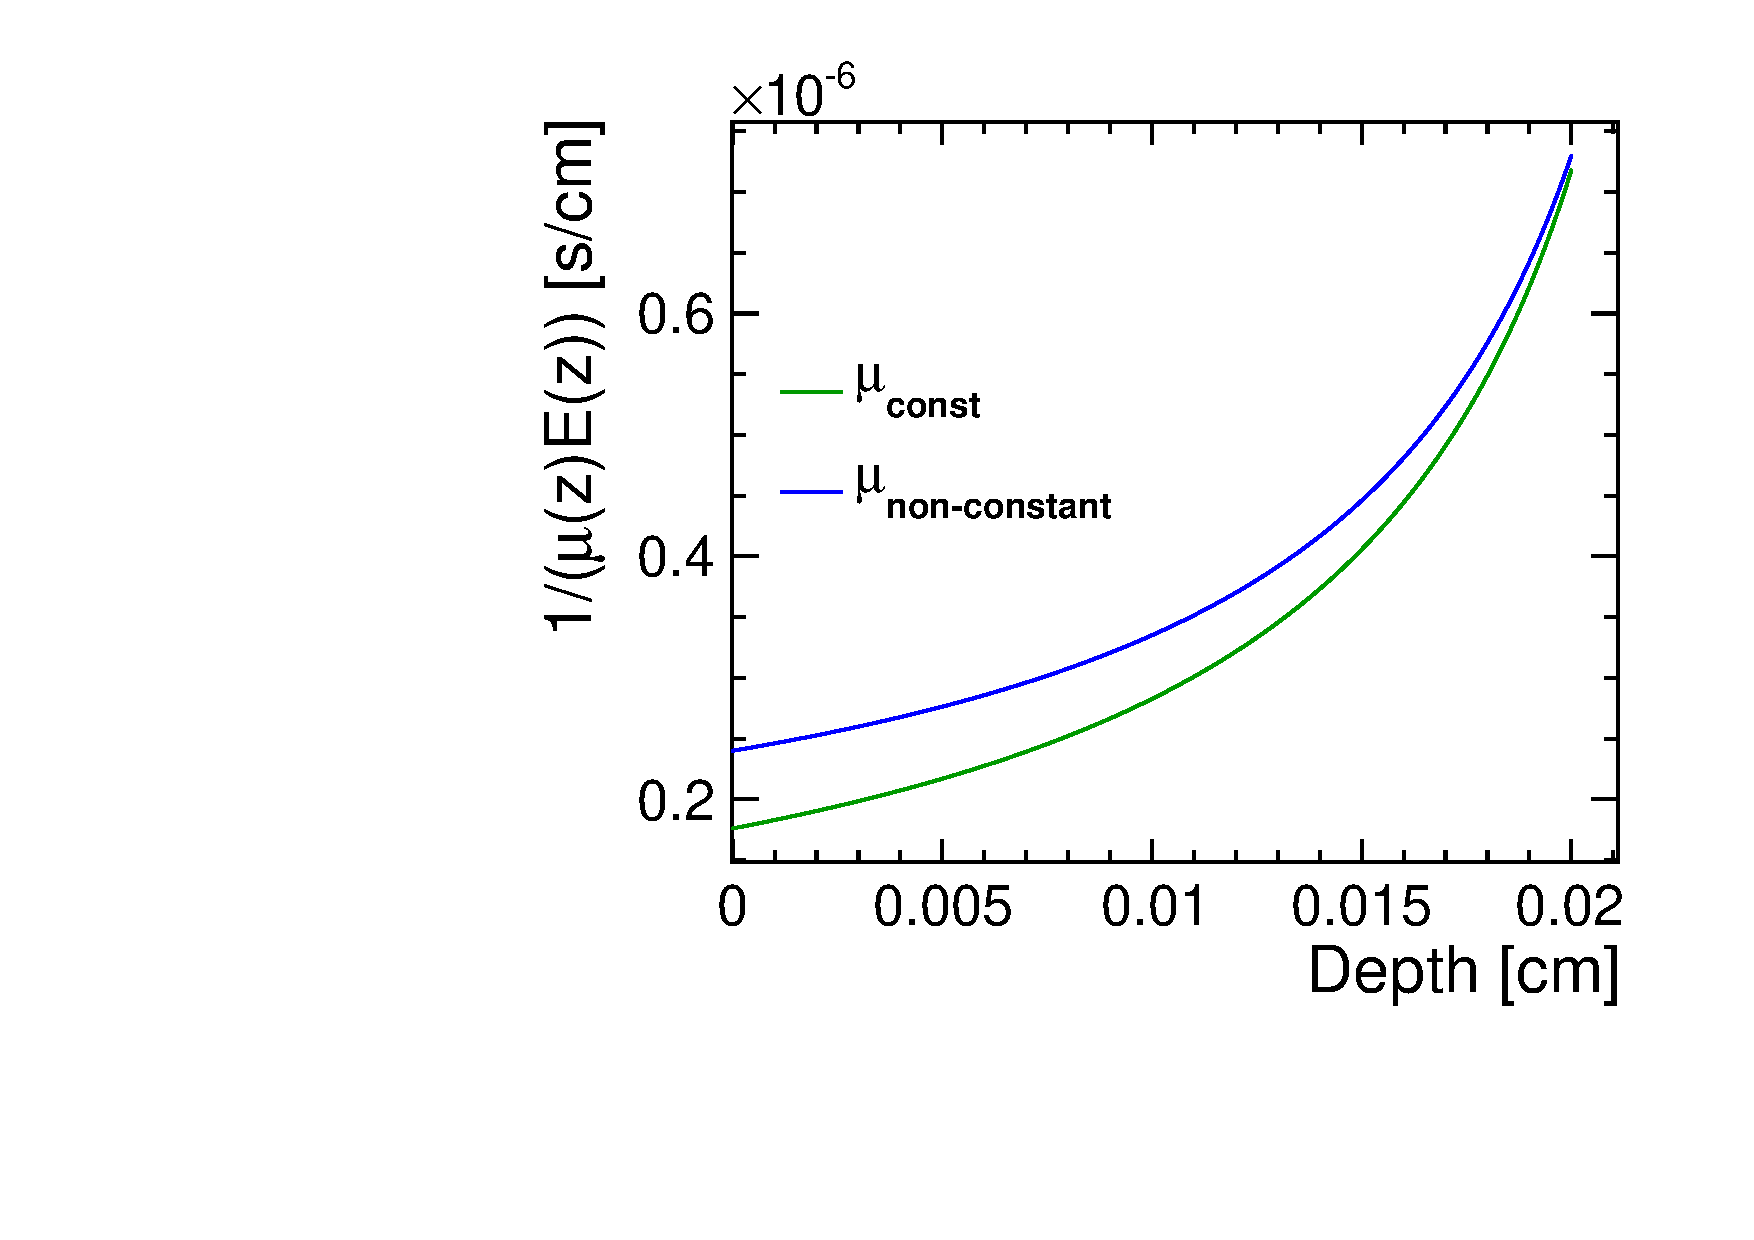
\includegraphics[width=\textwidth]{figures/ChargeSharing/B06_FunctionToIntegrate.pdf}
%%     \caption{}\label{fig:}
%%   \end{subfigure}\hfill
%%   \begin{subfigure}[b]{0.49\textwidth}
%%     \centering
%%     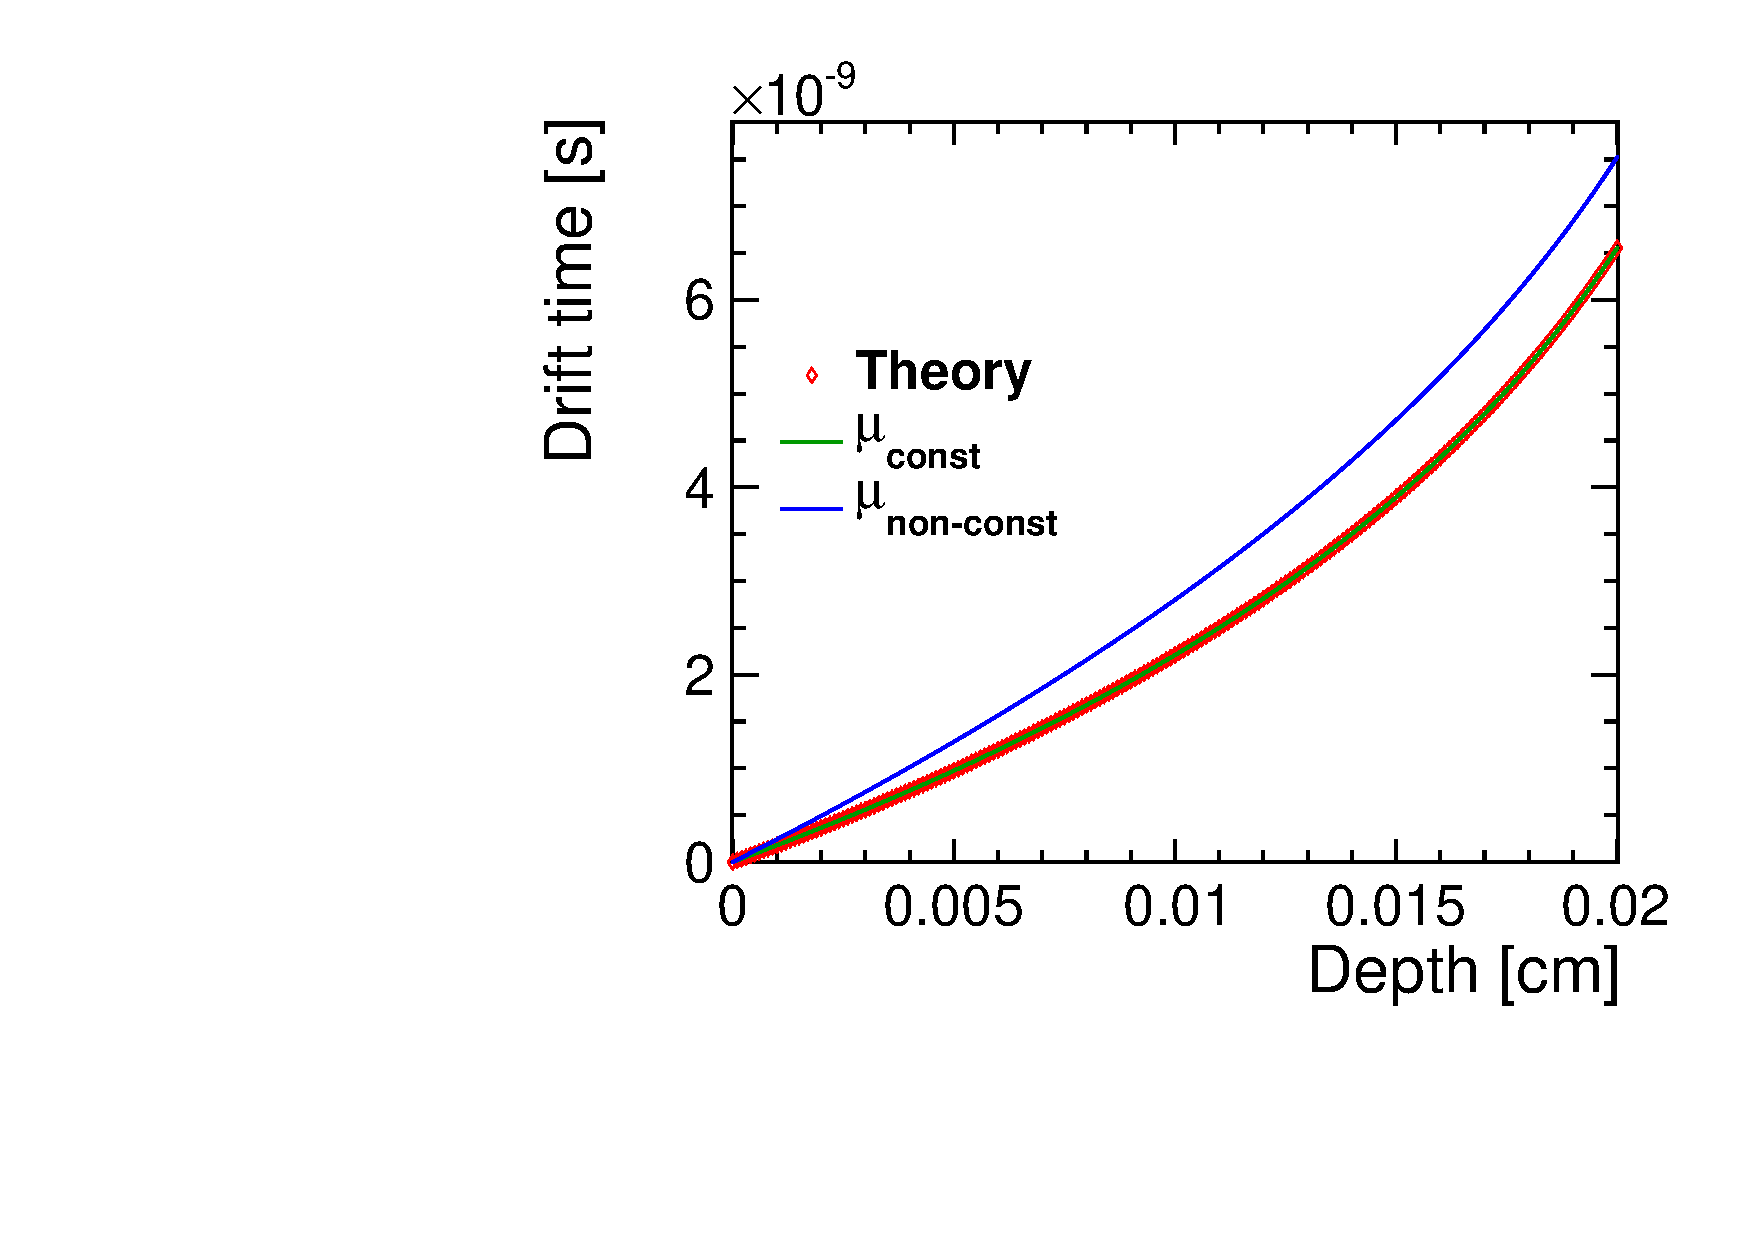
\includegraphics[width=\textwidth]{figures/ChargeSharing/B06_driftTime.pdf}
%%     \caption{}\label{fig:}
%%   \end{subfigure} 
%%   \caption{Drift time considering the mobility constant or non-constant.}\label{fig:}
%% \end{figure}

%% The diffusion constant and the diffusion spread considering the
%% mobility constant and non-constant.
%% \begin{figure}[htbp]
%%   \centering
%%   \begin{subfigure}[b]{0.49\textwidth}
%%     \centering
%%     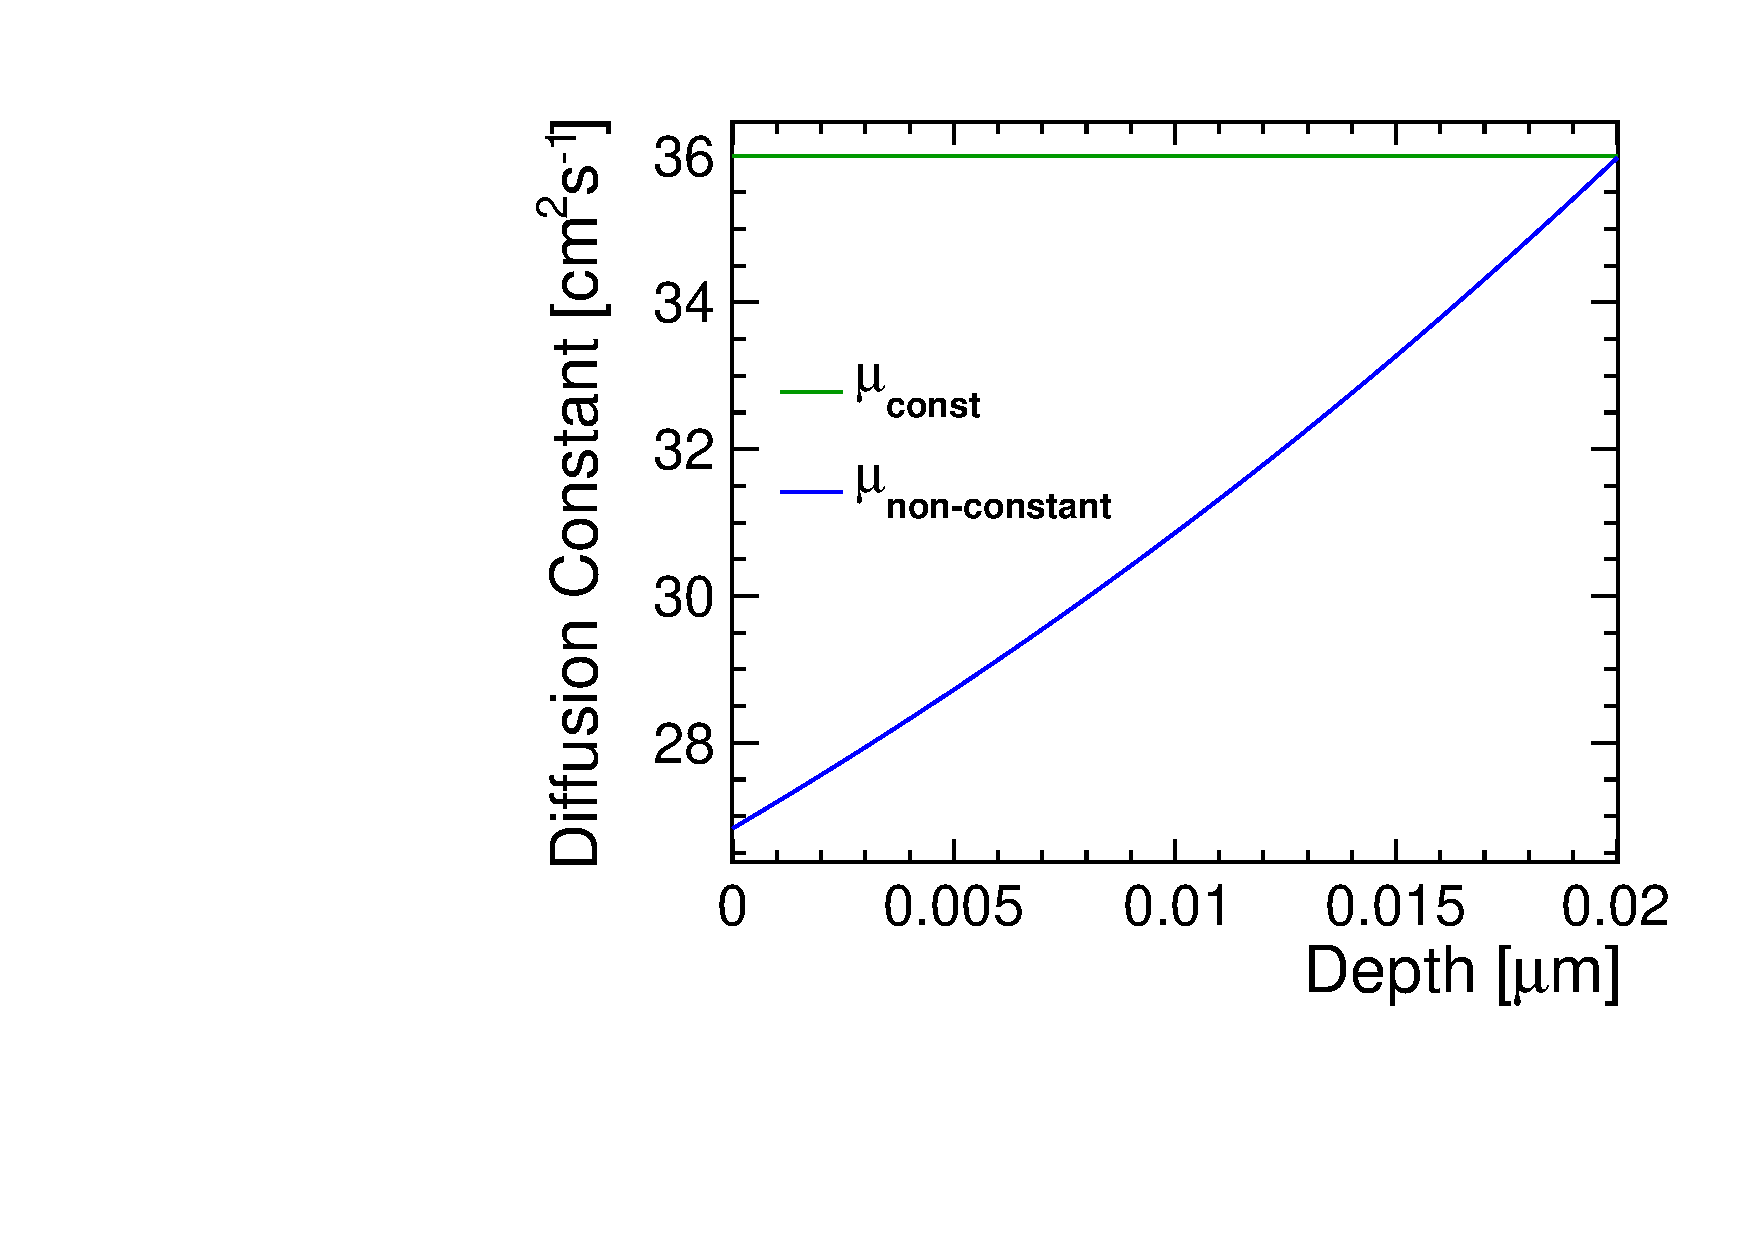
\includegraphics[width=\textwidth]{figures/ChargeSharing/B06_DiffusionConstant.pdf}
%%     \caption{}\label{fig:}
%%   \end{subfigure}\hfill
%%   \begin{subfigure}[b]{0.49\textwidth}
%%     \centering
%%     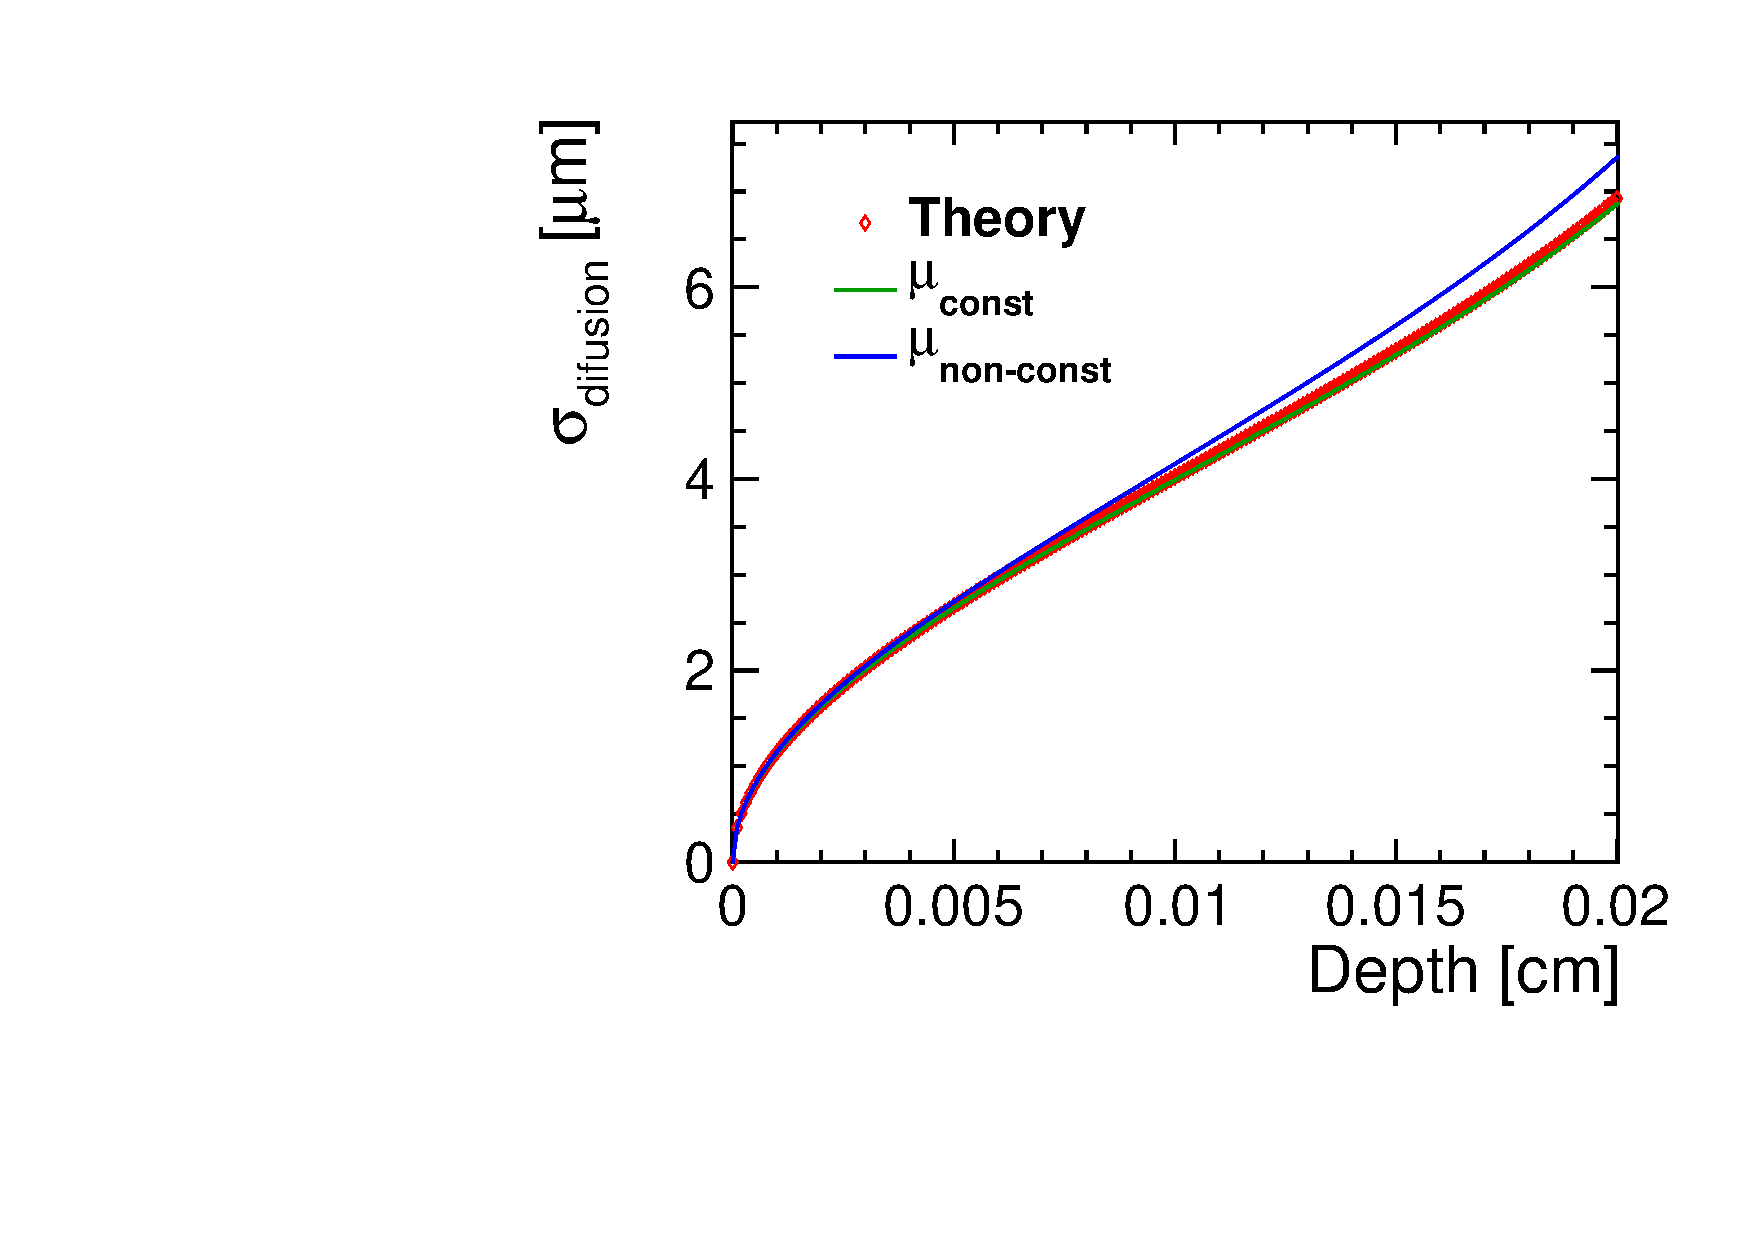
\includegraphics[width=\textwidth]{figures/ChargeSharing/B06_SigmaDiffusion.pdf}
%%     \caption{}\label{fig:}
%%   \end{subfigure} 
%%   \caption{The diffusion constant and spread for a constant mobility
%%     and a mobility which depends on the electric field. }\label{fig:}
%% \end{figure}

%% Comparing TCAD simulations and the charge sharing obtained by the
%% theoretical calculations gives us the following for a 200~\micron with
%% a depletion voltage of 30.31~V. Comparing for two different bias
%% voltages of 35~V and 50~V. In the case of the TCAD
%% simulations these results depend largely on the mesh divisions and
%% their locations. Both TCAD and theory assume a charge deposition of
%% 80e- per \micron.

%% \begin{figure}[htbp]
%%   \centering
%%   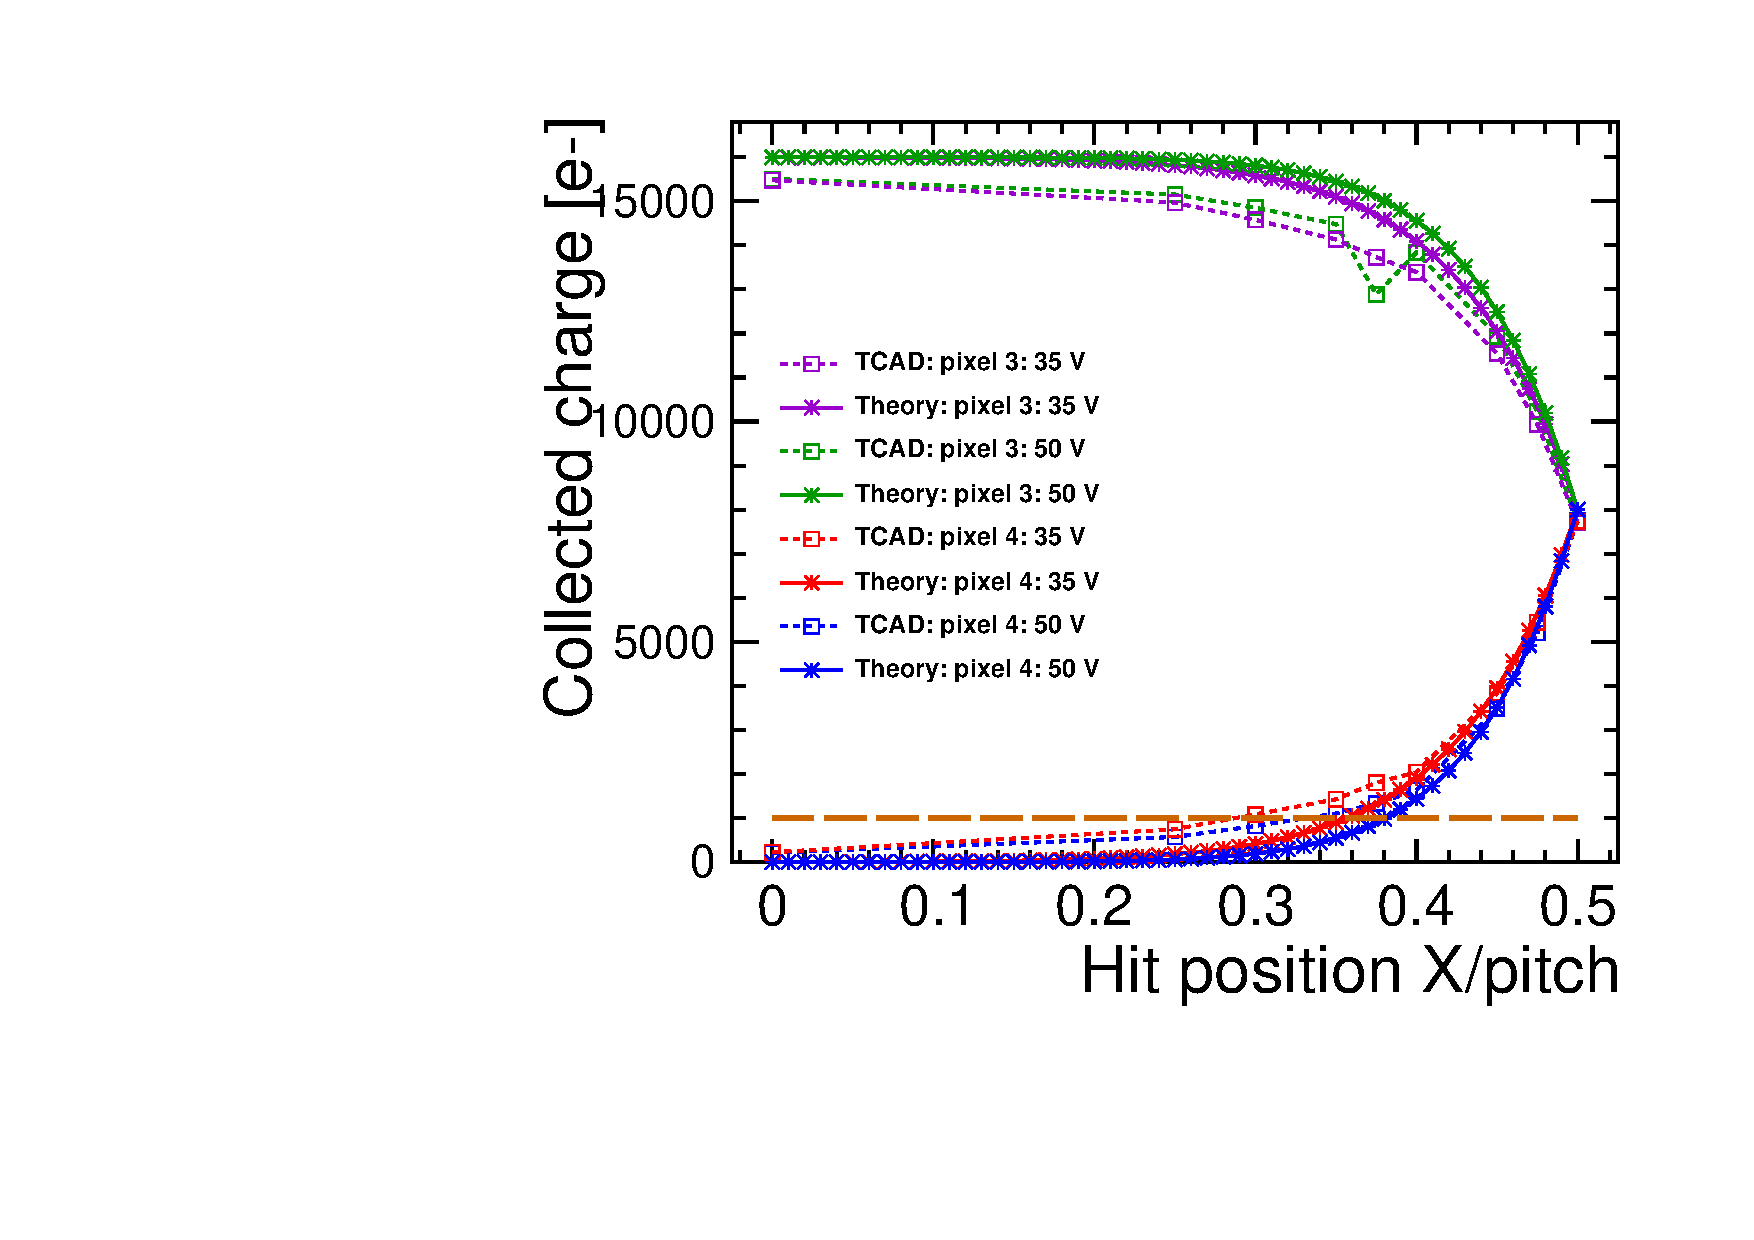
\includegraphics[width=0.5\textwidth]{figures/ChargeSharing/tcad_vs_theory.pdf}
%%   \caption{Diffusion comparing TCAD and theory.}\label{fig:}
%% \end{figure}

%==============================================================================    
\chapter{Pixel chip electronics and calibration}
\label{ch:FE_electronics}
%==============================================================================    

% ----------------------------- %
\tikzstyle{block} = [rectangle, draw, text width=5em, text centered, rounded corners, minimum
height=4em]
\usetikzlibrary{backgrounds,fit,decorations.pathreplacing} 
% ----------------------------- %

One of the key components of the detector systems is the readout
electronics. Each experiment, depending on the requirements, has its
own specific electronics. But the basic principles of the electronics
and optimisations of the signal-to-noise remain similar between
different applications.

In this chapter, we will review the basic principles and requirements
of the Timepix3 hybrid pixel readout chip which are used to study thin
and active-edge sensors as described in the following chapters. The
calibration method for the Timepix3 ASICs and also the noise
measurements are explored in this chapter.

%\section{Generic pixel chip properties}
\section{The Timepix3 hybrid readout ASICs}
\label{sec:TimepixChip}

The hybrid readout chip acquires the short ionisation current pulses
generated in the sensor by the passing of a high energetic
particle. The electronics are responsible for shaping the time
response of the system in order to optimise the minimum detectable
signal, energy deposition in detector measurement, event rate,
time-of-arrival and insensitivity to the pulse shape. Finally, the
signal is digitised and stored. Robustness to radiation and low power
consumption are other important considerations to be addressed amongst
others.


%% Timepix3 description
%% \section{The Timepix readout chip families}\label{sec:TimepixReadout}
The Timepix~\cite{art:tmpx,Timepix3Poikela} hybrid pixel detector
readout chip family, designed by the Medipix collaboration, is a
general purpose front-end electronics and can measure precisely the
energy deposited in the sensor and also provides accurate timing
information. This chip is used in a wide range of applications such as
high energy physics and medical imaging. The Timepix3 ASICs are
deployed for the CLIC vertex detector R\&D to study the feasibility of
thin sensors and also active-edge sensors as described in the coming
chapters. 

\cref{fig:detectorFunctions} schematically shows the basic signal flow
in a Timepix3-like hybrid pixel detector. Both analogue and
digital circuitry are combined. 

The incident radiation deposits energy in the sensor and it is
converted to an electrical signal. A high rate of particles can be
handled in a semiconductor detector because the sensor pulse is very
short (few nanoseconds). Since the magnitude of the signal charge is
small and subject to statistical fluctuations (\cref{sec:chargeInSi}),
a charge sensitive preamplifier is needed to amplify the signal. The
preamplifier should be designed in such a way to minimise the
electronic noise. The sensor capacitance and the input capacitance of
the amplifier are the critical parameters to increase the
signal-to-noise ratio (SNR): the lower the capacitance, the higher the
SNR. The amplification is done with a tunable discharge current of the
Krummenacher amplifier architecture
(I\textsubscript{krum})~\cite{KRUMMENACHER1991527}.

After the preamplifier, the pulse shaper is responsible for the
improvement of the SNR. It modifies the frequency response of the
signal to improve the signal and attenuate the noise. Since this
operation reduces the bandwidth of the signal, the duration of the
pulse will increase. A detector must cope with a high rate of pulses,
the width of the pulse must be optimised in a way to reduce the
pile-up. I\textsubscript{krum} affects the slope of the pulse
discharge after shaping: the higher its value, the shorter the
pulse.

The discriminator is used to compare the signal level to a
threshold (a voltage) and to discriminate a signal from a background
noise. Both polarities (electrons and holes collection) are accepted
by the front end.

The analog-to-digital converter (ADC) converts a continuously varying
amplitude to discrete steps. When the pulse height passes a threshold
in a comparator, counters are incremented to measure the energy and
the timing of the signal for example.

\begin{figure}[htbp]
  \centering
  \begin{tikzpicture}[node distance = 2.5cm, auto]
    \begin{scope}[x={(image.south east)},y={(image.north west)}]

      \coordinate (input);
      \node [block, right of=input] (sens) {Sensor};
      \node [block, right of=sens] (preamp) {Preamplifier};
      \node [block, right of=preamp] (pulse) {Pulse shaping};
      \node [block, right of=pulse] (discr) {Discriminator};
      \node [block, right of=discr] (conv) {ADC converter};
      \coordinate[right of=conv] (output);

      \draw[arrows=->] (input) -- node [text
      width=2cm,midway] {Incident radiation} (sens);
      \draw[arrows=->] (sens) -- (preamp);
      \draw[arrows=->] (preamp) -- (pulse);
      \draw[arrows=->] (pulse) -- (discr);
      \draw[arrows=->] (discr) -- (conv);
      \draw[arrows=->] (conv) -- node [text width=1.5cm,midway]
      {Digital data bus} (output);

      % \draw[] (sens) -- (discr.south);
      \draw[decorate,decoration={brace, mirror}, thick] (sens.south) to
      node[below,below] (bracket) {Analogue}
      (discr.south);

      \draw[decorate,decoration={brace, mirror}, thick] (conv.south west) to
      node[below,below] (bracket) {Digital}
      (conv.south east);

    \end{scope}
  \end{tikzpicture}
  \caption{Schematic overview of basic signal flow in a hybrid pixel
    detector. The energy deposited in the sensor by the incident
    radiation is converted to an electrical signal. The signal is
    integrated in the preamplifier, shaped by the pulse shaper and
    compared to a programmable threshold by the discriminator. The
    analogue-to-digital converter (ADC) digitises the signal for
    storage and analysis.}  
  \label{fig:detectorFunctions}
\end{figure}


An overview on the Timepix3 readout chip is given
in~\cref{tab:timepixOverview}. It consists of a $256\times256$ pixel
matrix with pixels pitch of $55\,\micron$. This chip allows for three
operation modes: photon counting (PC), Time-over-threshold (TOT) and
Time-of-Arrival (TOA) measurements. In addition, Timepix3 allows for
simultaneous measurement of the TOT and the TOA.

\begin{table}[htbp]
  \centering
  \caption{Overview of the Timepix3 readout ASICs.}
  \label{tab:timepixOverview}
  \begin{tabular}{l c}
    \toprule
    Pixel Matrix& $256\times256$\\
    Pixel Pitch [\micron] & 55\\
    Technology & 130~nm CMOS\\
    Counter Depth & 10 bit TOT and 18
                            bit TOA \\
    Clock speed & up to 40~\megahertz for TOT and 640~\megahertz for
                  TOA \\
    Readout Type & Data driven \& frame based \\
    Electronic Noise without sensor & $<70$ e\textsuperscript{-} RMS\\
    \bottomrule
  \end{tabular}
\end{table}


In the photon counting mode, a counter is incremented each time a
photon hits the pixel and deposits an energy higher than the
programmable threshold.
 
\cref{fig:TOT_TOA_concept} schematically shows the energy and the
timing measurement of the signal. The Time-over-threshold (TOT) allows
for the measurement of the energy deposited in a pixel. The pulse is
amplified and the pulse shaper integrates the signal to form a step
pulse with a long approximately linear decay. The time above the
programmable threshold is proportional to the energy deposited and
during this time, the TOT counter is incremented.

The Time-of-Arrival (TOA) measures the arrival time of a hit and
therefore is used as a time stamping of the hits. When the amplifier
output exceeds the pixel threshold, the discriminator output rises and
the fast TOA (FTOA) counter counts until the rising edge of the
general clock. A combination of the TOA and the FTOA counters is used
as the timing information for the hits.

\begin{figure}[htbp]
  \centering
  \begin{tikzpicture}
    \begin{scope}[x={(image.south east)},y={(image.north west)}]
      % pulse
      \draw[-, thick] (0.1, 0.8) -- (0.2, 0.8);
      \draw[-, thick] (0.2, 0.8) -- (0.21, 0.98);
      \draw[-, thick] (0.21, 0.98) -- (0.22, 0.8);
      \draw[-, thick] (0.22, 0.8) -- (1, 0.8);

      % shaper
      \draw[-, thick] (0.1, 0.5) -- (0.2, 0.5);
      \draw[-, thick] (0.2, 0.5) -- (0.22, 0.7);
      \draw[-, thick] (0.22, 0.7) -- (0.8, 0.5);
      \draw[-, thick, dashed, green] (0.1, 0.55) -- (0.8, 0.55);
      \draw[-, thick] (0.8, 0.5) -- (1, 0.5);

      % comparator
      \draw[-, thick] (0.1, 0.3) -- (0.21, 0.3);
      \draw[-, thick] (0.21, 0.3) -- (0.21, 0.4);
      \draw[-, thick] (0.21, 0.4) -- (0.65, 0.4);
      \draw[-, thick] (0.65, 0.4) -- (0.65, 0.3);
      \draw[-, thick] (0.65, 0.3) -- (1, 0.3);

      \timing [] at (0.11, 0.2) {HLLHHLLHHLLHHLLHHLLHHLLHH};
      \draw[arrows=<->, thick](0.21, 0.15)--(0.65, 0.15) node [pos=0.5, below]
      {\textbf{TOT (3 counts)}};

      \timing [] at (0.1,0.0) {llllllhlhlhlhllllllllllllllllllllllllllllllllllllll};

      \draw[-, thick, dashed, blue] (0.21, 0.55) -- (0.21, 0.0);
      \draw[-, thick, dashed, blue] (0.65, 0.55) -- (0.65, 0.0);

      \draw[-, thick, dashed, red] (0.355, 0.2) -- (0.355, 0.0);

      \draw[arrows=<->, thick](0.21, -0.05)--(0.35, -0.05) node [pos=0.5, below]
      {\textbf{FTOA (4 counts)}};


      \node[left] at (0.1, 0.8) {Sensor pulse};
      \node[left, green] at (0.1, 0.6) {Threshold};
      \node[left] at (0.1, 0.5) {Pulse after shaping};
      \node[left] at (0.1, 0.3) {Discriminator output};
      \node[left] at (0.1, 0.2) {General clock}; %$40\,\megahertz$ Clk}
      \node[left] at (0.1, 0.0) {FTOA clock}; %$640\,\megahertz$ Clk (FTOA)     


    \end{scope}
  \end{tikzpicture}
  \caption{Schematic overview of the Time-over-Threshold (TOT) and
    Time-of-Arrival (TOA) measurements for the Timepix3 readout chips.}
  \label{fig:TOT_TOA_concept}
\end{figure}


\subsection{SPIDR readout system for Timepix3}\label{sec:TimepixReadout}

The SPIDR (Speedy PIxel Detector Readout) readout system has been
developed by NIKHEF and CERN is used~\cite{Visser:2015bsa} for the
Timepix3 data acquisition. This system is able to handle high rates of
data sent by the Timepix3 ASIC at full speed. This is achieved with
Xilinx Virtex-7 FPGA~\cite{XilinxVirtex7} and a 10~Gb Ethernet link.

\begin{figure}[htbp] \centering
  \begin{subfigure}[b]{0.3\textwidth}
    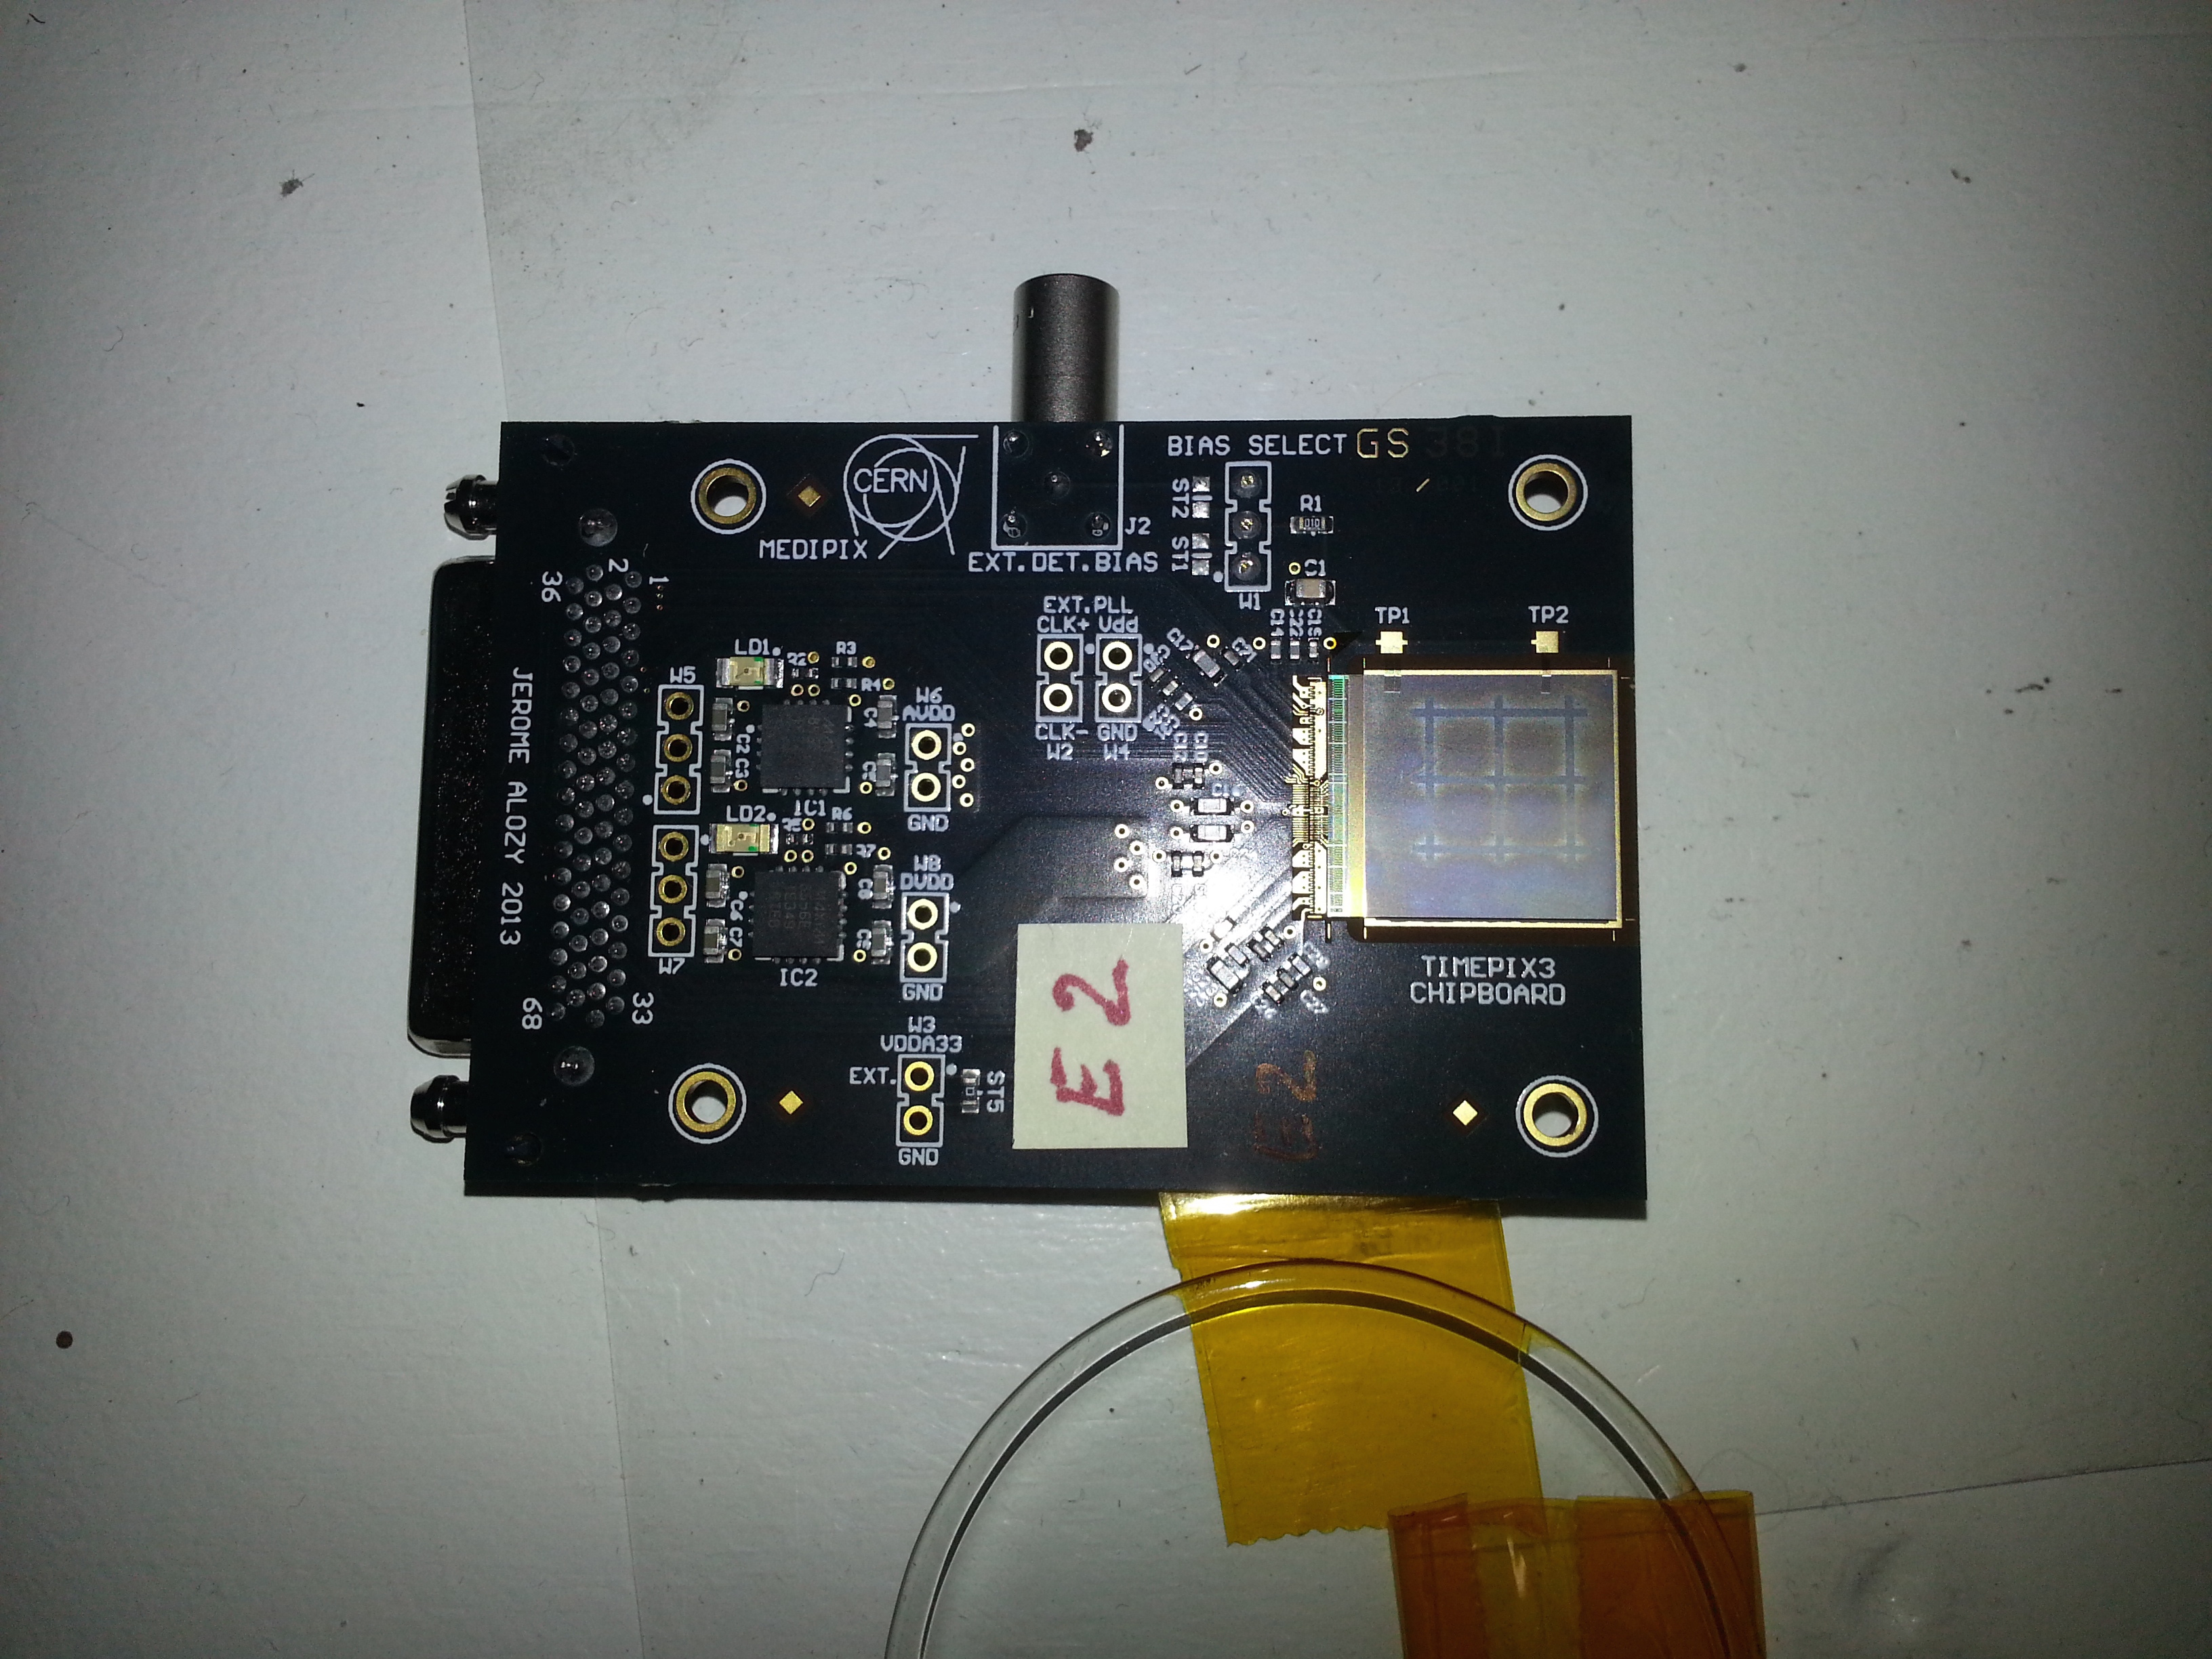
\includegraphics[width=\textwidth]{./figures/Calibration/Timepix3board.jpg}
    \caption{}\label{fig:Timepix3board_PCB}
  \end{subfigure}\hfill
  \begin{subfigure}[b]{0.65\textwidth}
    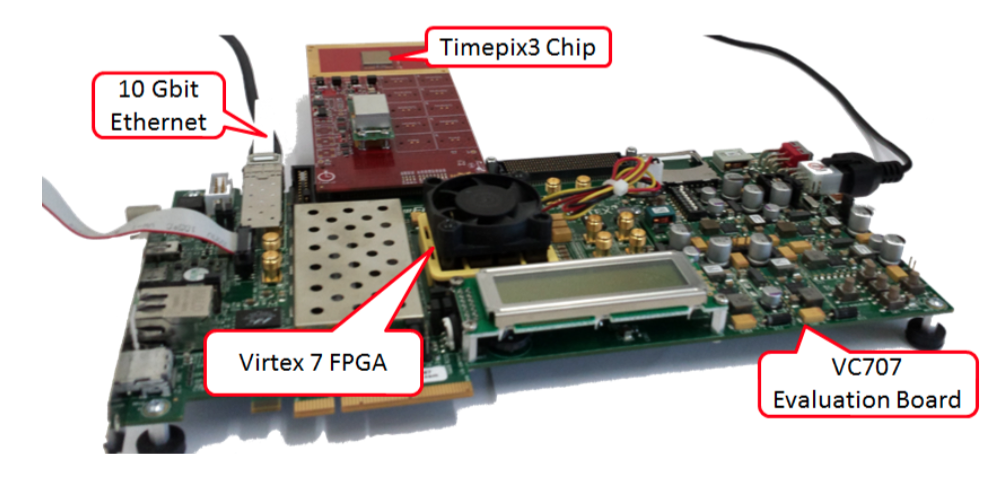
\includegraphics[width=\textwidth]{./figures/Calibration/SPIDRboard.png}
    \caption{}
  \end{subfigure}
  \caption{(a) Timepix3 chip board and (b) SPIDR readout board.}
  \label{fig:Timepix3board_SPIDR}
\end{figure}

The Timepix3 readout chip allows for a data-driven zero-suppressed
readout mode which can reach higher readout rates than the frame based
mode. In the data driven mode, after a hit is processed by the pixel,
a data packet containing the TOT and the TOA information is
immediately sent off the chip. This reduces significantly the dead
time of the pixels and allows to reach very high readout rates of up
to 40~Mhits/s/\cmsquared.

The different settings of the chip are controlled externally using
programmable DACs such as the I\textsubscript{krum}, threshold,
polarity of the sensor and the clock speed.

%% --------------------------------------------- %%
\section{Timepix3 assemblies}\label{sec:Timepix3Assemblies}
A summary of the Timepix3 assemblies is shown in
\cref{tab:Timepix3Assemblies}. Advacam sensors~\cite{AdvacamRef} of
thickness $50$-$300\,\micron$ are bump-bonded to Timepix3 readout
chips.

\begin{table}[htbp]
  \centering
  \caption{Details of different Advacam planar pixel sensors
    bump-bonded to Timepix3 readout ASICs and studied in calibration
    and test beams. For active-edge sensors, the edge distance is
    defined by the distance between the last pixel implant and the
    physical sensor edge.}
  \label{tab:Timepix3Assemblies}
  \resizebox{\textwidth}{!}{\begin{tabular}{lccccc}
    \toprule
    Timepix3 ID & Thickness [\micron] & Type & Edge distance [\micron] & Guard-ring potential & Assembly\\
    \midrule
     W19\_G7 & 50 & n-in-p & 20 & Without GR & 20-NGR-50 \\
     W19\_F7 & 50 & n-in-p & 23 & Floating & 23-FGR-50 \\
     W19\_L8 & 50 & n-in-p & 28 & Grounded & 28-GNDGR-50 \\
     W19\_C7 & 50 & n-in-p & 55 & Grounded & 55-GNDGR-50 \\ \hline
     W5\_E2 & 100 & n-in-p & 55 & Grounded & 55-GNDGR-100 \\ \hline
     W5\_F1 & 150 & n-in-p & 55 & Grounded & 55-GNDGR-150 \\ \hline
     W2\_J5 & 300 & p-in-n & - & - & - \\
    \bottomrule
  \end{tabular}}
\end{table}

%% --------------------------------------------- %%
\section{Electronic noise}\label{sec:noise}

Electronic noise places a limit on the minimum detectable signal
level, defines the ability to distinguish signal levels and their
precision of measurement. Thermal excitations and sensor leakage
currents are important sources for the noise. The electronic noise can
be measured as explained further in
\cref{sec:thresholdCalibration}. For Timepix3 readout chips, the
electronic noise before bonding to any sensor is less than
70~e\textsuperscript{-} RMS and after bonding it increases to
$\sim80$~e\textsuperscript{-} RMS due to the capacitance of the sensor
and its leakage current.

The electronic noise is an important parameter to determine the
operating threshold of the readout chip. In fact, the operating
threshold for the Timepix3 chip is set to 6 times the electronic noise
RMS. This threshold significantly reduces the detection of noisy
hits. Sometimes at this threshold few pixels show a high rate of hits
in absence of incident radiation (hot pixels) and they are manually
masked to be able to operate the chip at the lowest possible
threshold.

The operating threshold affects significantly the spatial resolution
of the device. A lower threshold allows for a higher detection of the
charge sharing. For this reason, it is important to minimise the
electronic noise.

%% --------------------------------------------- %%
\section{Threshold dispersion and equalisation} 
\label{sec:ThresholdEqualisation}


In semiconductor electronics, manufacturing imperfections cause
variations in the performance within the device. The programmable
global threshold of the chip is one of the most affected
parameters. In fact, the global threshold is programmed through a
programmable DAC (Digital-to-Analog) and is translated to the voltage
applied at the discriminator. The signal level is compared to this
voltage. For the same global threshold value, the voltage on the
discriminator can vary highly from one pixel to another. To overcome
this dispersion, a 4-bit local threshold adjustment is applied to each
pixel in order to make a uniform global threshold. The photon counting
mode is then employed. The equalisation consists of adjusting this
local threshold. First it is set to its minimum value (mask 0000). The
global threshold DAC (THL) is scanned and the number of pixels
responding are counted. Then the adjustment bit is set to its maximum
value (mask 1111) and THL is scanned again. For each pixel, the
operation range is thus known. Assuming a linear relationship between
the two points, the adjustment threshold is adjusted in such a way
that the global threshold will remain uniform across the matrix.

\cref{fig:THLequalisation} shows the threshold equalisation for the
assembly W2\_J5. After equalisation the response of the chip becomes
more uniform even though some dispersion remains.

\begin{figure}[htbp] 
  \centering
  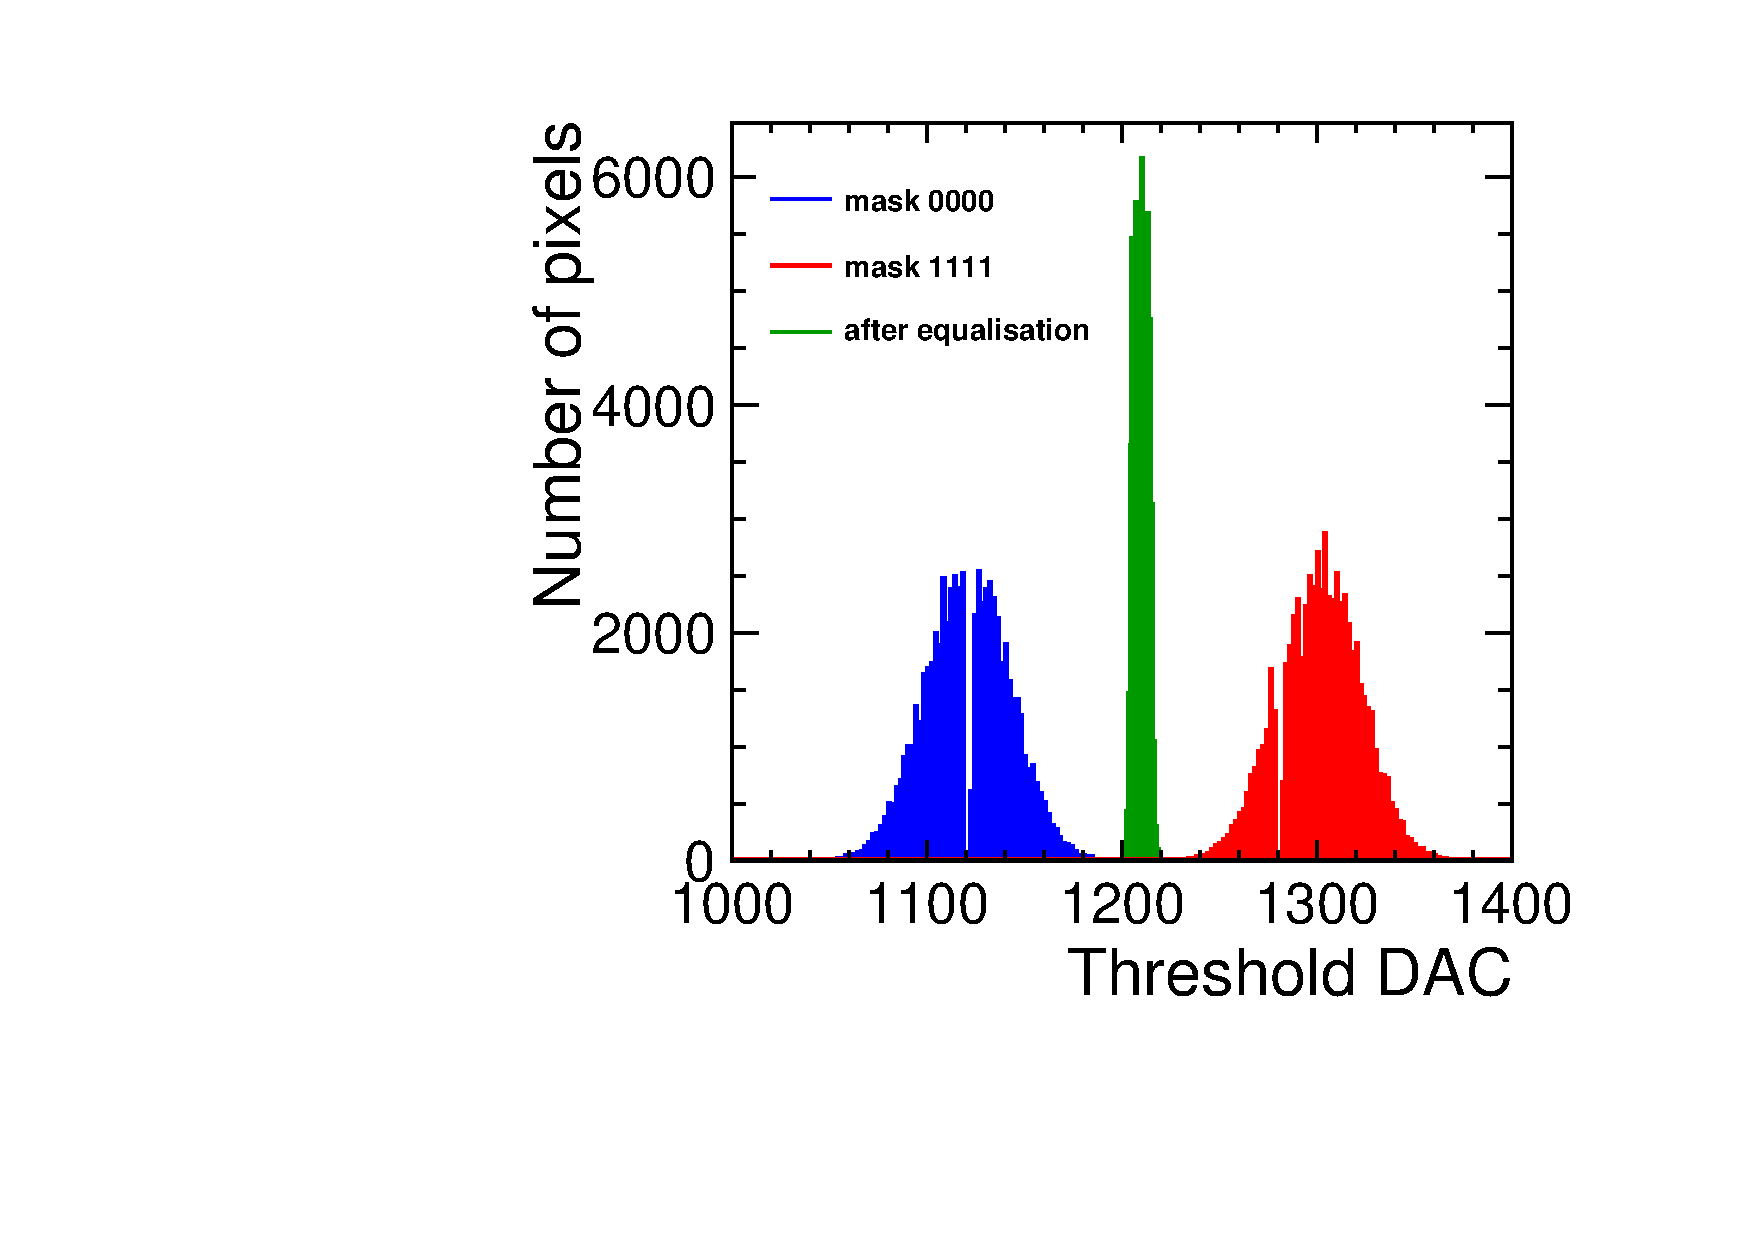
\includegraphics[width=0.6\textwidth]{./figures/Calibration/THLequalisation_W2_J5.pdf}
  \caption{Spread of pixel responses for the assembly W2\_J5 during
    equalisation for the local threshold set at its minimum value
    (mask 0000), to its maximum value (mask 1111) and after
    equalisation.}
  \label{fig:THLequalisation}
\end{figure}

\section{Calibration} \label{sec:calibration} The aim of the
calibration is to parametrise the measurements done by the readout
chip, namely the relationship between the threshold DAC and the TOT
with the energy deposited in the sensor (in number of collected
charge) as well as the relation between the TOA measurement and the
time of arrival of the particle (in seconds). In this work we focus on
the threshold DAC and the TOT calibration.

The threshold DAC and TOT calibration can be achieved using two main
methods. The first one consists of the use of photons from radioactive
sources with a characteristic decay energy or photons from X-ray
fluorescence (XRF) with a characteristic emission
energy~\cite{AlipourTehrani:2054922}. The photon being stopped in the
sensor, it deposits its full energy. Since the energy of the photon is
known, its relation to the threshold DAC or TOT can be characterised. 

The second method consists of the use of an internal analog test pulse
generator. The Timepix3 readout ASICs provide an internal test pulse
generator which can be used for calibration as well as equalisation of
the readout chip. In each pixel, a capacitor allows for injecting a
charge by switching a voltage over it. The charge injected is given by

\begin{equation}
  Q = C \cdot \Delta V \; ,
  \label{eq:testpulseCharge}
\end{equation}

where Q is the injected charge, C the injection capacitance and
$\Delta V$ the voltage applied. A priori, the injection capacitance is
unknown and its value varies from pixel to pixel, but its value can be
measured. For the capacitance, $20.2$~e\textsuperscript{-}/mV is a
good approximation.

In \cref{fig:detectorFunctions}, the injection capacitance replaces
the sensor. For the calibration if the chip is bump-bonded to a
sensor, the sensor is fully depleted with a bias voltage.

\subsection{TOT-energy calibration} \label{sec:EnergyCalibration}

The TOT calibration parametrises the relationship between the energy
deposited (in number of electrons) and the TOT measurement. Due to the
non-linearity of the Timepix3 charge preamplifier, this relationship
is modeled as a hyperbola. The function used to fit the data points is
called a \textit{surrogate function} and is defined as:

\begin{equation}
  \text{TOT} = a \, E + b - \frac{c}{E - t} \; ,
  \label{eq:TOTsurrogateFunction}
\end{equation}

where TOT denotes Time-Over-Threshold, $E$ the energy and $a, b, c, t$
are the parameters to be found~\cite{Jakubek2008155}. The inverse of
the surrogate function is defined as:

\begin{equation}
  E = { {t \cdot a - \text{TOT} -b + \sqrt{\left(b+t \cdot a -\text{TOT}\right)^2+4\cdot a \cdot c}} \over {2a} } \; ,
  \label{eq:inverseTOTsurrogateFunction}
\end{equation}

In \cref{eq:TOTsurrogateFunction}, for higher values of the energy,
the relationship between TOT and $E$ is linear with gradient $a$ and
intercept $b$ since the term $aE+b$ dominates. At low energy, the term
$c/(E-t)$ becomes important. The parameter $c$ defines the amount of
curvature in the function. An asymptote occurs at $E=t$. The point at
which the fit crosses the x-axis (TOT=0) corresponds to the threshold:
below the threshold no charge can be detected. The range for the TOT
and the boundary between low energy (non-linear response) and high
energy (linear response) depend on the clock frequency, the threshold
and the I\textsubscript{krum} value.

For the calibration of the assemblies, the Timepix3 ASICs is operated
in the TOT mode and the test-pulse injection is used
(\cref{eq:testpulseCharge}). Test pulses with heights ranging from
$0\,\mv$ to $800\,\mv$ (corresponding to 0 electrons to 14000
electrons) are sent to each pixel. For each pulse height, 100
test-pulses are sent. The sum of the TOTs and also the sum of the
squared of the TOTs for each pulse height is recorded. The mean of the
TOT response and the standard deviations are then calculated. Finally,
the data are fitted with the surrogate function as given in
\cref{eq:TOTsurrogateFunction} for each pixel and the pixel-by-pixel
energy calibration of the assembly is determined.

\cref{tab:timepix3Operation} summarises the DAC settings used for the
operation of the Timepix3 assemblies in test beams. The same settings
are as well used for the calibration. \cref{fig:TOTcalib_55GNDGR100}
shows the pixel-by-pixel calibration for assembly W5\_E2 operated at
two different threshold DACs of 1160 and 1190. For a higher threshold,
the curves are shifted towards higher energy values on the x-axis but
the slope (parameter $a$) remains the same.

\begin{table}[htbp]
  \centering
  \caption{DAC settings for the operation and calibration of the
    Timepix3 assemblies. VFBK is a programmable DAC to determine the
    baseline voltage of the chip.}
  \label{tab:timepix3Operation}
  \begin{tabular}{ c c c c }
    \toprule
    I\textsubscript{krum} & TOT/TOA Clock & FTOA Clock & VFBK \\
    \midrule
    10 & $40\,\megahertz$ & $640\,\megahertz$ & 150 \\
    \bottomrule
  \end{tabular}
\end{table}

\begin{figure}[htbp] \centering
  \begin{subfigure}[b]{0.45\textwidth}
    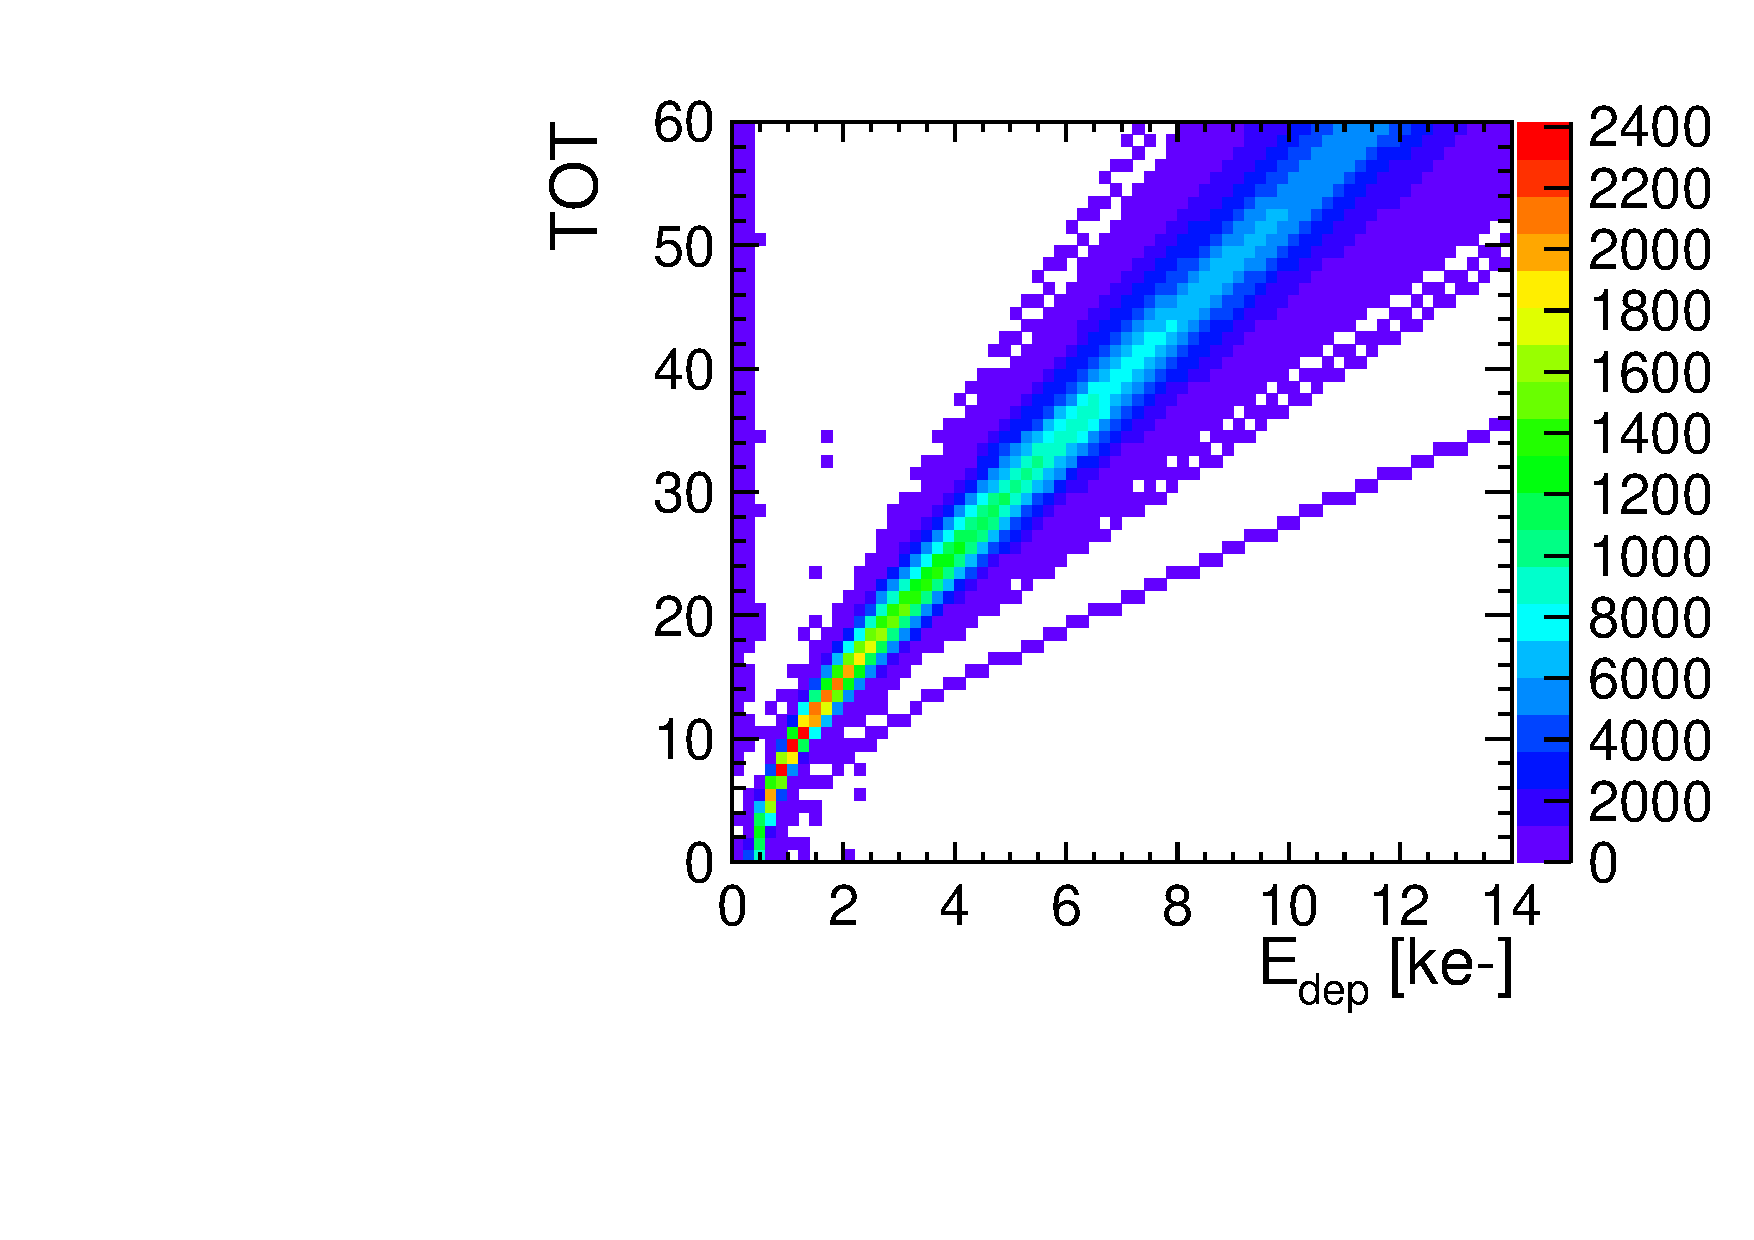
\includegraphics[width=\textwidth]{./figures/Calibration/TOTcalibration_W0005_E02_thresh1160.pdf}
    \caption{}
  \end{subfigure} \hfill
  \begin{subfigure}[b]{0.45\textwidth}
    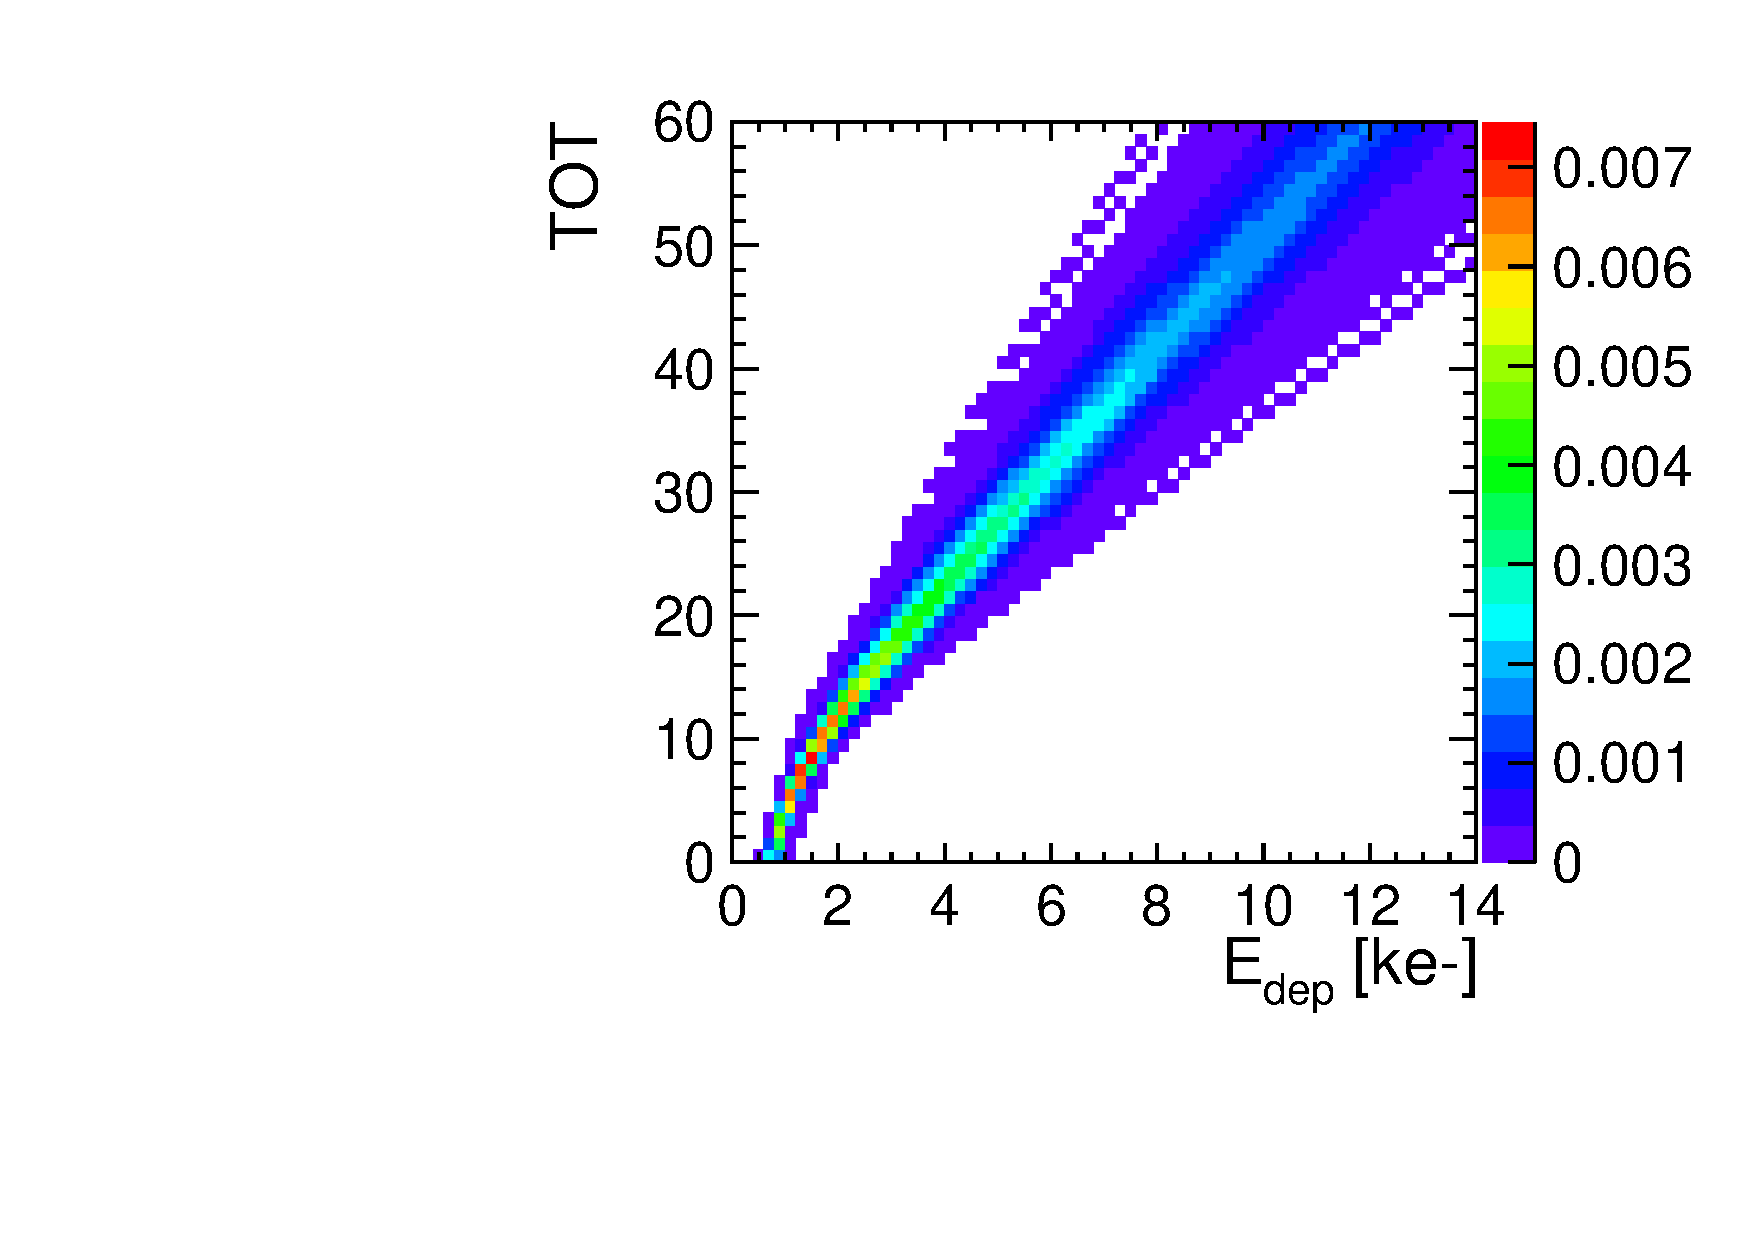
\includegraphics[width=\textwidth]{./figures/Calibration/TOTcalibration_W0005_E02_thresh1190.pdf}
    \caption{}
  \end{subfigure}
  \caption{Pixel-by-pixel calibration of the TOT for assembly W5\_E2
    operated at the threshold DACs of (a) THL=1160 and (b) THL=1190.}
  \label{fig:TOTcalib_55GNDGR100}
\end{figure}

The calibration for the other assemblies are given in
\cref{sec:appendixFE_electronics}.


\subsection{Threshold-energy calibration} 
\label{sec:thresholdCalibration}

\cref{sec:noise} describes the selection of the operating threshold
DAC (Digital-to-Analog Converter) for a Timepix3 readout chip. This
threshold can be translated into an effective energy and used as a
data point for the surrogate fit at the crossing-point on the
$x$-axis. The counting mode is used for this measurement.

For Timepix3 assemblies, the threshold is calibrated using test pulses
at four different heights corresponding to 0, 1000, 3000 and 6000
electrons. For each pulse height, 200 pulses are sent to the pixels in
the diagonal of the matrix and the threshold DAC is scanned with a
step of 2 from a level of no counts (threshold above the signal) to a
level where all the pixels count (threshold close to the noise level)
resulting in an S-shaped curve as shown in
\cref{fig:scurve_example}. The readout electronics noise smears the
ideal sharp turn on and generates the S-curve. At the maximum gradient
of the S-curve, the threshold DAC corresponds to the pulse
amplitude. The derivative of the S-curve is a Gaussian as shown in
\cref{fig:deriv_example} with a mean at the maximum gradient of the
S-curve. The derivative at each point of the S-curve corresponds to
the slope of the line connecting it to its neighbour.

\begin{figure}[htbp] \centering
  \begin{subfigure}[b]{0.45\textwidth}
    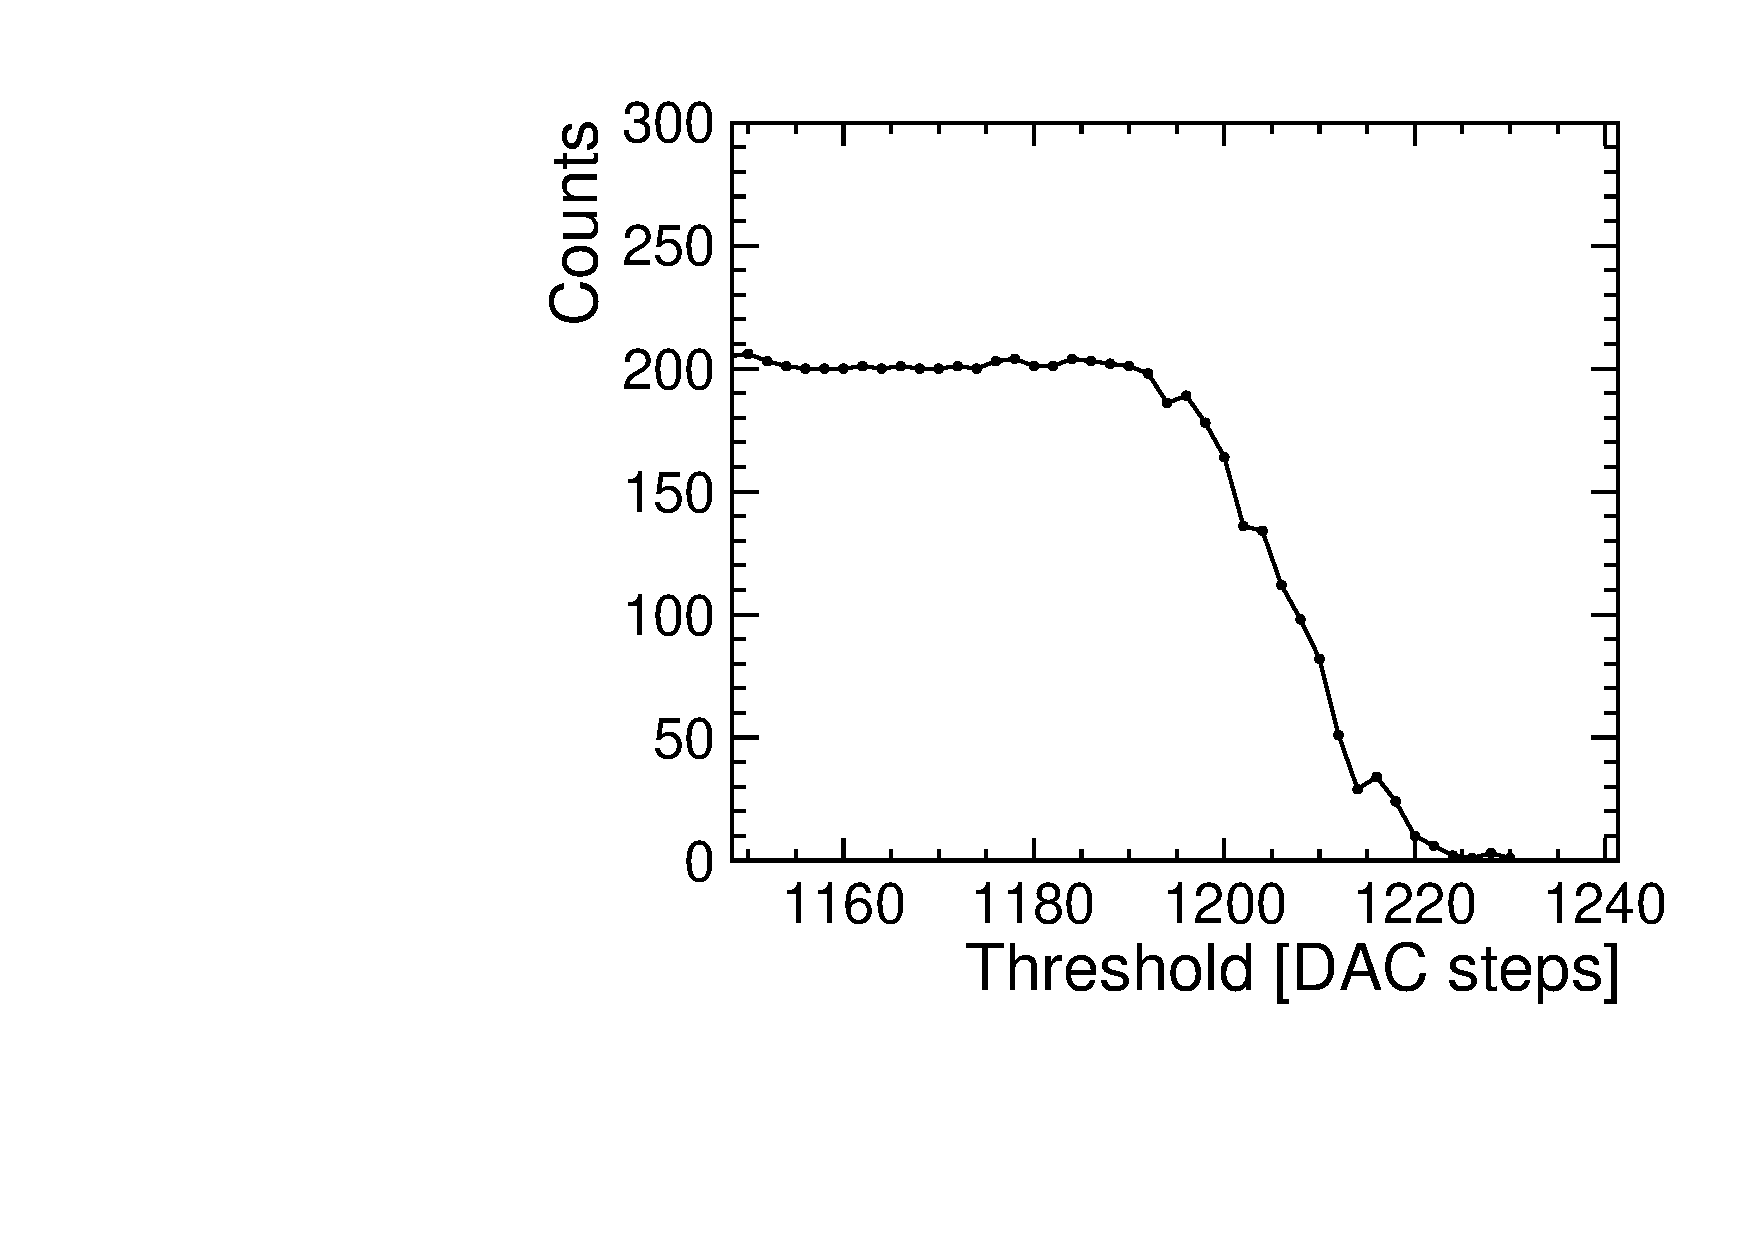
\includegraphics[width=\textwidth]{./figures/Calibration/W5_E2_scurve_ampl1.pdf}
    % \begin{tikzpicture} \node[anchor=south west,inner sep=0] (image)
    %   at
    %   (0,0){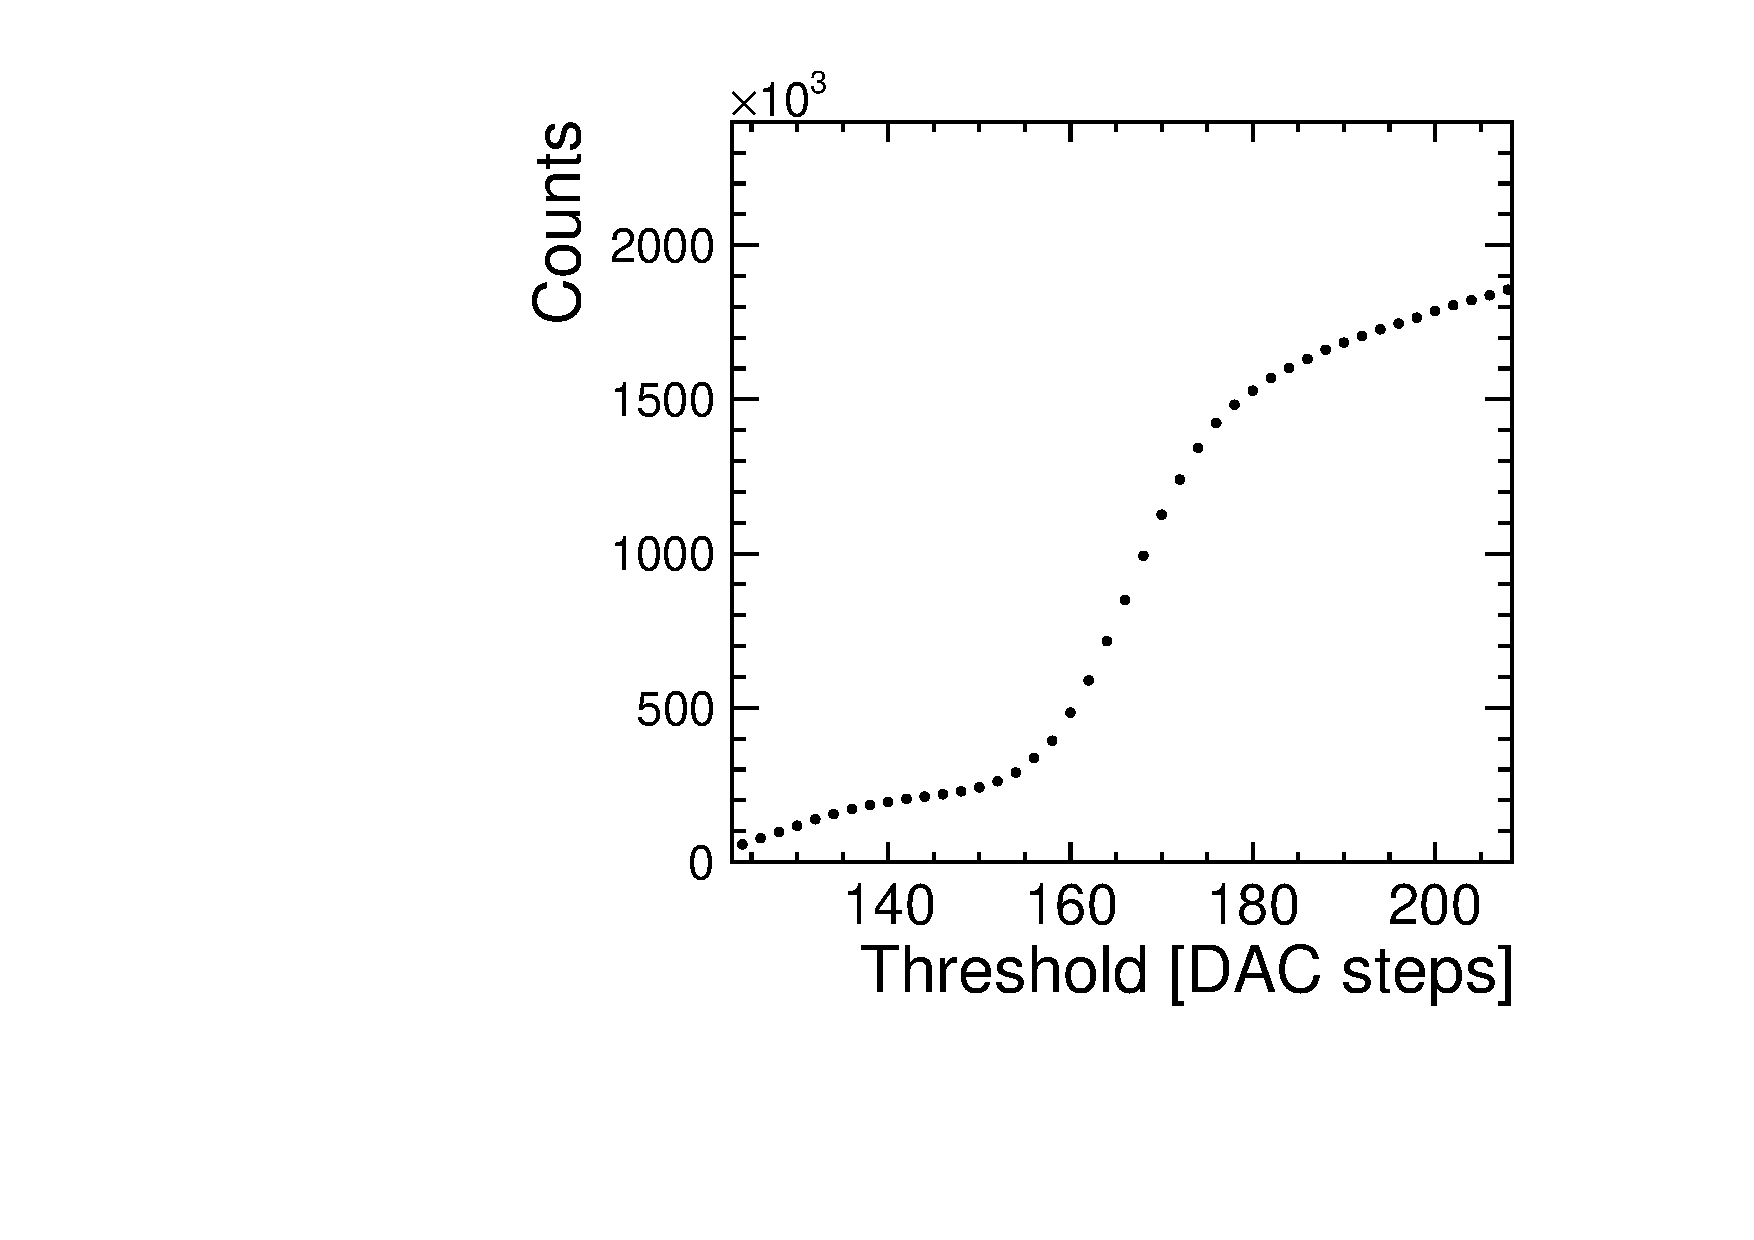
\includegraphics[width=\textwidth]{./figures/Calibration/L04-W0125_scurve_In.pdf}};
    %   % \draw[->,line width=.4pt, color=black](1.8, 1.4) -- (2.4, 1.4);
    %   \node[left, color=black] at (1.9, 1.6) {$K_{\beta}$}; %\draw[->,line
    %   width=.4pt, color=black](3, 2.7) -- (3.7, 2.7); \node[left,
    %   color=black] at (3.5, 2.7) {$K_{\alpha}$};
    % \end{tikzpicture}
    \caption{Measured S-curve}
    \label{fig:scurve_example}
  \end{subfigure} \hfill
  \begin{subfigure}[b]{0.45\textwidth}
    % 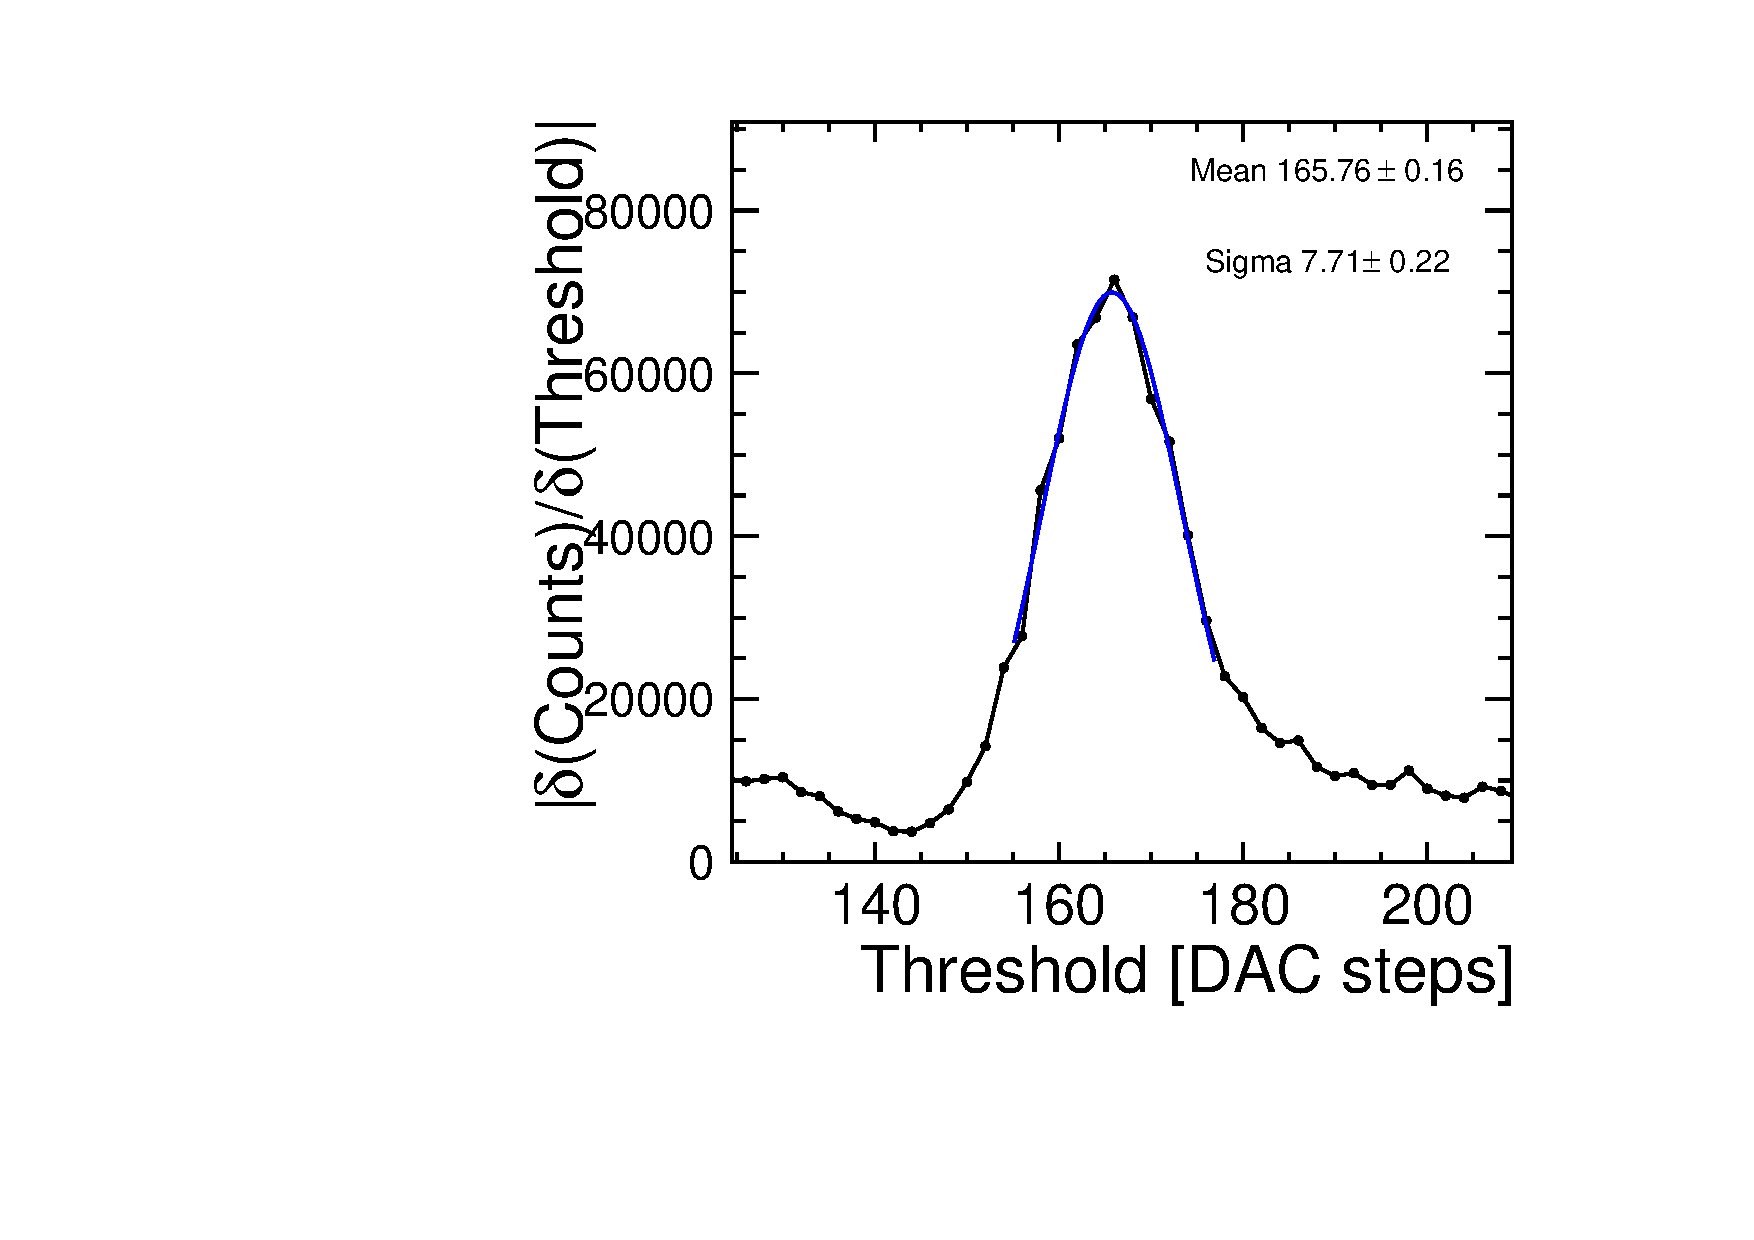
\includegraphics[width=\textwidth]{./figures/Calibration/L04-W0125_scurveDeriv_In.pdf}
    \includegraphics[width=\textwidth]{./figures/Calibration/W5_E2_deriv_scurve_ampl1.pdf}
    \caption{Derivative of the S-curve}
    \label{fig:deriv_example}
  \end{subfigure}
  \caption{An example of a measured S-curve (a) and its derivative
    fitted with a Gaussian function (b) for the assembly W5\_E2 using
    a pulse height of 1000 electrons for the pixel (0, 0). This
    measurement is performed for all the pixels on the diagonal of the
    matrix for each assembly. The threshold DAC is scanned with a step
    size of 2.}
  \label{fig:scurve_deriv_example}
\end{figure}

A linear fit is used to parametrise the relationship between the pulse
height and the threshold DAC given by the mean of the derivative of
the S-curves:
\begin{equation}
  THL_{DAC}=p \; THL_{e-} + q \; ,
  \label{eq:THLDAC}
\end{equation}
where $THL_{DAC}$ is the threshold DAC setting and $THL_{e-}$ the
corresponding energy (in number of electrons). 

\cref{fig:THLcalib_55-GNDGR-100} shows an example of the threshold
calibration obtained for the assembly W5\_E2. Each point used for the
fit corresponds to the mean of the Gaussian fitted to the derivative
of the S-curve for each pulse height. The error on each point
corresponds to the error on the mean of the fitted Gaussians of all
diagonal pixels combined using the propagation of errors.

\begin{figure}[htbp]
  \centering
  \includegraphics[width=0.5\textwidth]{./figures/Calibration/THLcalibration_W0005_E02.pdf}
  \caption{Threshold calibration for W5\_E2. Each point corresponds to
    the maximum gradient of the S-curve for each pulse height. A
    linear function as described in \cref{eq:THLDAC} was used to fit
    the data points and obtain the parameters $p$ and $q$.}
  \label{fig:THLcalib_55-GNDGR-100}
\end{figure}

% \begin{figure}[htbp]
%   \centering
%   \includegraphics[width=0.5\textwidth]{./figures/Calibration/A06-W0110_THLcalibration.pdf}
%   \caption{Threshold calibration for A06-W0110. Each point corresponds
%     to the maximum gradient of the S-curve for each target (Cu, Zr, Pd
%     and In). A linear function as described in \cref{eq:THLDAC} was
%     used to fit the data points and obtain the parameters $p$ and
%     $q$.}
%   \label{fig:THLcalib_A06}
% \end{figure}

The operating threshold DAC for each assembly was converted to an
energy by solving \cref{eq:THLDAC} for $THL_{e-}$ with
$THL_{DAC}=THL_{DAC}^{op}$. The error on the evaluated threshold in energy
($THL_{e-}^{op}$) is obtained by the propagation of errors for the
inverse of \ref{eq:THLDAC}:
\begin{equation}
  \sigma_{THL_{e-}}^2(THL_{DAC})={{{(THL_{DAC}-q)^2} \over {p^4}} \sigma_{p}^2} +
        {\frac{1}{p^2} \sigma_{q}^2}+
        {2 {{THL_{DAC}-q} \over p^3} \sigma_{pq}^2} \; ,
        \label{eq:THLerror}
\end{equation}
where $p$, $q$ are given by the linear fit using \cref{eq:THLDAC} with
standard deviations $\sigma_{p}$, $\sigma_{q}$ and covariance
$\sigma_{pq}$.

\cref{tab:THLcalibration} summarises the fit parameters p and q, the
operating threshold DAC and its conversion into energy deposition in
number of electrons for all the assemblies listed in
\cref{tab:THLcalibration}.

\begin{table}[htbp]
  \centering
  \caption{Threshold fit parameters p and q, the operating threshold
    DAC and its conversion into energy deposition.}
  \label{tab:THLcalibration}
  \begin{tabular}{lcccc}
    \toprule
    Assembly & p [DAC steps/e\textsuperscript{-}] & q [DAC steps] & THL\textsubscript{DAC}\textsuperscript{op} [DAC steps] & THL\textsubscript{e-}\textsuperscript{op} [e\textsuperscript{-}] \\
    \midrule
    W19\_G7 & $0.087\pm0.000$ & $1144.037\pm0.005$ & 1190 & $526.230\pm0.649$ \\
    W19\_F7 & $0.092\pm0.000$ & $1131.874\pm0.009$ & 1187 & $600.406\pm0.551$ \\
    W19\_L8 & $0.090\pm0.000$ & $1082.057\pm0.005$ & 1133 & $568.506\pm0.538$ \\
    W19\_C7 & $0.091\pm0.000$ & $1092.887\pm0.005$ & 1148 & $608.700\pm0.488$ \\
    W5\_E2 &  $0.095\pm0.000$ & $1106.921\pm0.004$ & 1160 & $561.019\pm0.712$ \\
    W5\_F1 & $0.089\pm0.000$ & $1103.618\pm0.004$ & 1153 & $554.885\pm0.493$ \\
    W2\_J5 & $-0.109\pm0.000$& $1232.643\pm0.034$ & 1170 & $565.723\pm1.560$\\
    \bottomrule
  \end{tabular}
\end{table}



For further verification of these results, the Timepix3 DAC step gain
for each assembly is calculated to be around
11~$\pm$e\textsuperscript{-}/step, in agreement
with~\cite{Timepix3Poikela}. 

Without any test-pulse injection, the threshold scan results in a
Gaussian distribution. The mean of the Gaussian distribution defines
the baseline of the chip and its width, the electronic noise. For all
assemblies the noise varies between 6 to 7 DAC values which
corresponds to 70 to 80 electrons, again in agreement
with~\cite{art:tmpx} (the error is obtained by error propagation of
\cref{eq:THLDAC}). Except for the assembly W2\_J5 which appears to be
noisy. \cref{tab:THLcalibration_noise} summarises the baseline mean,
the threshold DAC step, the electronic noise and its conversion into
energy deposition for the assemblies listed in
\cref{tab:THLcalibration}.


%%%%%%%%%%%%%%%%%%%%%%%%%%%%%%%%%%%%%%%%%%%%%%%%%%

\begin{table}[htbp]
  \centering
  \caption{Measured baseline mean, threshold DAC step gain, the electronic noise
    and its conversion into energy deposition.}
  \label{tab:THLcalibration_noise}
  \resizebox{\textwidth}{!}{\begin{tabular}{lcccc}
    \toprule
    Assembly & Baseline mean [DAC steps] & Threshold DAC step [e\textsuperscript{-}] & Noise [DAC steps] & Noise [e\textsuperscript{-}] \\
    \midrule
    W19\_G7 & $1143.992\pm0.005$ & $11.450\pm0.000$ & $6.864\pm0.005$ & $78.585\pm0.056$ \\
    W19\_F7 & $1131.664\pm0.009$ & $10.892\pm0.000$ & $7.060\pm0.009$ & $76.891\pm0.098$ \\
    W19\_L8 & $1081.998\pm0.005$ & $11.160\pm0.000$ & $6.996\pm0.005$ & $78.078\pm0.058$ \\
    W19\_C7 & $1092.825\pm0.005$ & $11.044\pm0.000$ & $7.413\pm0.005$ & $81.870\pm0.051$ \\
    W5\_E2  & $1106.895\pm0.004$ & $10.570\pm0.000$ & $7.155\pm0.004$ & $75.628\pm0.046$ \\
    W5\_F1  & $1103.591\pm0.004$ & $11.237\pm0.000$ & $6.711\pm0.004$ & $75.408\pm0.046$ \\
    W2\_J5  & $1231.70\pm0.034$ & $-9.177\pm0.000$ & $11.826\pm0.041$ & $108.53\pm0.379$ \\
    \bottomrule
  \end{tabular}}
\end{table}

%%%%%%%%%%%%%%%%%%%%%%%%%%%%%%%%%%%%%%%%%%%%%%%%%%%%%%%%
%%%%%%%%%%%%%%%%%%%%%%%%%%%%%%%%%%%%%%%%%%%%%%%%%%%%%%%%
%%%%%%%%%%%%%%%%%%%%%%%%%%%%%%%%%%%%%%%%%%%%%%%%%%%%%%%%
% \begin{table}[htbp]
%   \caption{Measured DAC step gain.}
%   \label{tab:DACStep}
%   \centering
%   \begin{tabular}{ c c c }
%     \toprule
%     Assembly & Threshold DAC step [\ev] & Threshold DAC step [\Pem] \\
%     \midrule
%     A06-W0110  & $81\pm0.009$ & $22.475\pm0.025$  \\
%     C04-W0110  & $85\pm0.039$ & $23.544\pm0.011$ \\
%     L04-W0125 &  $86\pm0.022$ & $23.775\pm0.006$ \\
%     B06-W0125  & $86\pm0.120$ & $23.978\pm0.033$ \\
%     \bottomrule
%   \end{tabular}
% \end{table}

% Threshold measurements were not completed for assemblies B07-W0125 and
% D09-W0126. Assembly B07-W0125 did not fully deplete due to a broken
% corner of the sensor. The derivative of the CuXRF S-curve did not form
% a peak as the photon energy was close to the noise level. Assembly
% D09-W0126 was not operating as expected for a $100\,\micron$
% sensor. Therefore the calibration of these assemblies was done without
% threshold measurements.



%% \begin{table}[htbp]
%%   \centering
%%   \caption{Advacam active-edge n-in-p planar pixel sensor assemblies. The edge distance is defined by the distance between the last pixel implant and the physical sensor edge.}
%%   \label{tab:NominalThreshold}
%%   \resizebox{\textwidth}{!}{\begin{tabular}{lccc}
%%       \toprule
%%       Assembly & Nominal THL\textsubscript{DAC}\textsuperscript{op} [DAC steps] & Nominal THL\textsubscript{e-}\textsuperscript{op} [electrons]\\
%%       \midrule
%%       20-NGR & 1190 & 466.5\\
%%       23-FGR & 1187 & 532.4\\ \hline
%%       28-GNDGR & 1133 & 517.8\\
%%       55-GNDGR & 1148 & 553.7\\
%%       55-GNDGR-100 & 1160 & 537.9\\ \hline
%%       55-GNDGR-150 & 1153 & 441.2\\
%%       \bottomrule
%%   \end{tabular}}
%% \end{table}


% \begin{table}[htbp]
%   \caption{Threshold fit parameters $p$ and $q$, the operating
%     threshold DAC and its conversion into energy.}
%   \label{tab:evalTHL} 
%   \centering
%   \begin{tabular}{ c c c c c }
%     \toprule
%     Assembly & $p$ [DAC steps/\kev] & $q$ [DAC steps] & $THL_{DAC}^{op}$ [DAC steps] & $THL_{\kev}^{op}$ [\kev] \\
%     \midrule
%     A06-W0110 & $-12.36\pm0.03$ & $364.0\pm0.50$ & 326 & $3.077\pm0.033$ \\
%     C04-W0110 & $-11.8\pm0.02$ & $441.6\pm0.42$ & 405 & $3.102\pm0.030$ \\
%     L04-W0125 & $-11.68\pm0.02$ & $448.6\pm0.31$ & 410 & $3.303\pm0.023$ \\
%     B06-W0125 & $11.58\pm0.037$ & $390.6\pm0.80$ & 435 & $3.836\pm0.057$ \\
%     \bottomrule
%   \end{tabular}
% \end{table}

% ==============================================================================
\chapter{Simulation and reconstruction software frameworks}
\label{sec:Software}
%==============================================================================    

Simulation tools have a crucial role in the development and also
understanding of the performance of semiconductor devices. The
simulations are validated with the data and used to predict the
performance of small-pitch pixels where data is unavailable. 

This chapter describes the simulation tools used to understand the
performance of Timepix3 devices. The reconstruction software (for data
and simulation) is also presented.

%% --------------------------------------------- %%
\section{\textsc{Geant4}}\label{sec:Silicon_Geant4}

\textsc{Geant4}~\cite{Agostinelli:2002hh}, as an object-oriented
simulation toolkit implemented in C++ programming language, is widely
used in high energy, nuclear and accelerator physics, medical and
space sciences. As the modern particle physics is going towards
large-scale detectors, more accurate simulations are needed in order
to understand the complex situations. \textsc{Geant4} provides
software components which can be used to study basic phenomena,
geometries and full-scale detector simulations for
experiments. \textsc{Geant4} simulations take into account parameters
such as: the geometry of the system, the materials involved, the
fundamental particles, the generation of primary particles, the
tracking of particles through materials and external electromagnetic
fields, the physics processes involved in the possible interaction of
the particles with the materials they are passing through, the
response of sensitive components and mostly validated with data.

\textsc{Geant4} provides physics models for different type of
interactions called \textit{physics lists}. The \textit{emstandard}
physics lists provide the electromagnetic interactions of photons and
charged particles with matter and is suited for the simulation of
ionisation, bremsstrahlung, gamma conversion and other electromagnetic
interactions of particles with energies from $1\,\kev$ up to
$10\,\pev$~\cite{Apostolakis2009859}. This physics list is commonly
used for the simulation of the energy loss in pixel detectors.

\textsc{Geant4} provides as well the Photo-Absorption Ionisation (PAI)
model~\cite{Apostolakis:2000yu} for the precise simulation of
ionisation energy loss by relativistic charged particles in very thin
absorbers. Since in very thin sensors the Landau model is not
suitable, the PAI model is based on the photo-absorption cross-section
tables obtained by experimental data. In practice several classes are
used to calculate the integral ionisation cross-section, the mean
number of ionising collisions as well as the mean ionisation energy
loss for the selected material and the given Lorentz factor.

\cref{fig:BichselVSG4} compares the energy loss due to ionisation in
$50\,\micron$ and $450\,\micron$ thick silicon sensors for different
\textsc{Geant4} physics lists and the Bichsel model
(c.f. \cref{sec:bichsel}). \textsc{Geant4} version 10.1.2 is used to
obtain these distributions. Version 9.6.2 also showed the same
results. For $50\,\micron$ thick sensor, the \textit{emstandard\_opt3}
physics list gives a reasonable value for the $\Delta_p$ but the width
$w$ of the distribution is more narrow than the Bichsel
distribution. The PAI model corrects for $w$ and the energy deposition
is very similar to the Bichsel model. For the thick sensor of
$450\,\micron$, both PAI and emstandard\_opt3 physics lists show
similar distributions as the Bichsel model.

The energy deposition given by the PAI model is very close to the one
calculated by Bichsel especially for the fluctuations around the most
probable value and for very thin sensors. For this reason, the PAI
model is chosen to be used later for the simulations even though it
requires more computation power.
 
\begin{figure}[htbp] \centering
  \begin{subfigure}[b]{0.45\textwidth}
    \includegraphics[width=\textwidth]{figures/ChargeSharing/50um_bichsel_physicsLists.pdf}
    \caption{}
  \end{subfigure} \hfill
  \begin{subfigure}[b]{0.45\textwidth}
    \includegraphics[width=\textwidth]{figures/ChargeSharing/450um_bichsel_physicsLists.pdf}
    \caption{}
  \end{subfigure}
  \caption{Energy-loss distribution in (a) $50\,\micron$ and (b)
    $450\,\micron$ thick silicon sensors by $120\,\gev$ $\pi^{+}$
    comparing the Bichsel model and \textsc{Geant4} using the PAI and
    the emstandard\_opt3 physics lists.}
  \label{fig:BichselVSG4}
\end{figure}

%% --------------------------------------------- %%
\section{AllPix simulation framework}
\label{sec:AllPix}

AllPix~\cite{allpix} is a \textsc{Geant4}-based simulation
software. It is written in C/C++ and provides a flexible interface to
define any pixel detector geometry to simulate pixelated sensors and
readout chips.

The pixel detectors are placed in the world volume. \textsc{Geant4}
provides the simulation of particles through the matter: it calculates
the position of the hits (or the Monte Carlo Truth position)
considering the multiple scatterings and the energy deposition in the
sensitive volumes (sensors). The software user defines the
semiconductor physics and readout chip properties in a digitiser as
described here below.

\cref{fig:TPX3TelescopeAllpix} shows an example of the simulation for
the Timepix3 telescope (described in \cref{ch:Telescope}) in AllPix
with the device under test (DUT) in the middle of the rotated telescope
planes.

\begin{figure}[htbp]
  \centering
  \begin{tikzpicture}
    \node[anchor=south west,inner sep=0] (image) at
    (0,0){\includegraphics[width=0.8\textwidth]{figures/ActiveEdge/Allpix_telescope_withParticles.png}};
    \begin{scope}[x={(image.south east)},y={(image.north west)}]
      \node[above, color=white] at (0.45, 0.65) {\textbf{DUT}};
    \end{scope}
  \end{tikzpicture}
  \caption{Simulation of the Timepix3 telescope with AllPix.}
  \label{fig:TPX3TelescopeAllpix}
\end{figure}

%% --------------------------------------------- %%
\subsection{Coordinate system}

The convention used for the pixel detectors (in AllPix but also the
reconstruction software as described in \cref{sec:recoSoft}) for a
Timepix3-like matrix of $256\times256$ pixels is shown in
\cref{fig:coordinateSystem}. The pixel coordinates (X, Y) and the
\textcolor{blue}{local coordinates (x, y) in millimeters} of the
center of the pixels in the corners of the matrix are shown. In this
convention we are looking from the sensor side with the periphery on
the top.

\begin{figure}[htbp]
  \centering
  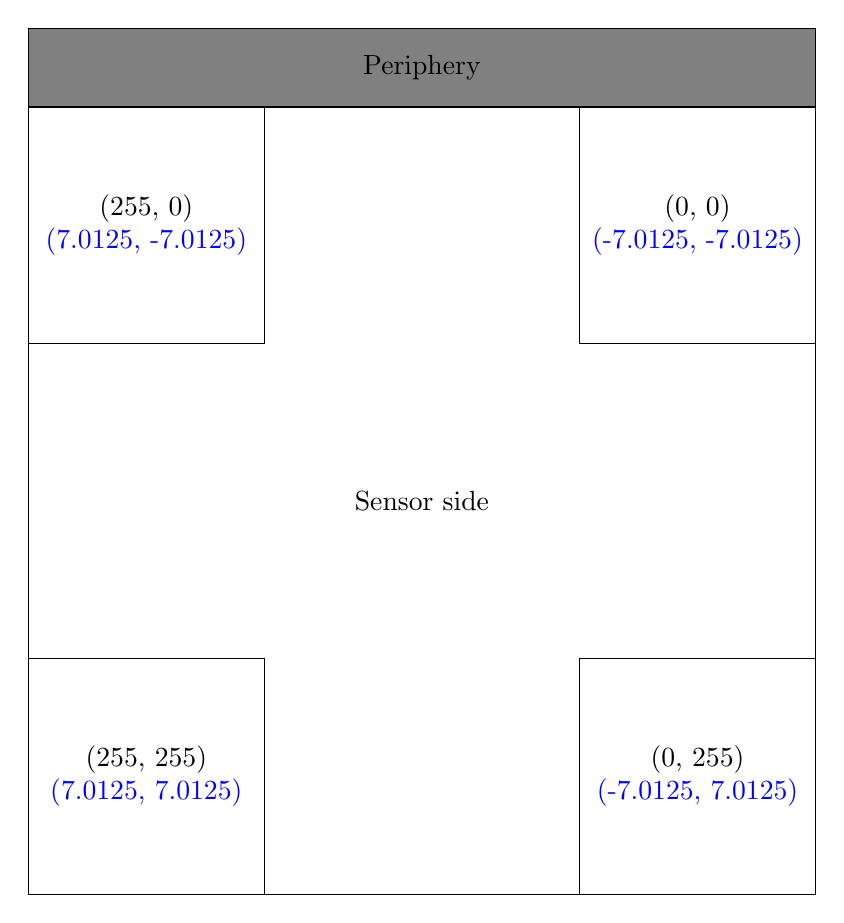
\begin{tikzpicture}
    \begin{scope} 

      \draw (0, 0) rectangle (10, 10) node[pos=.5] {Sensor side};
      \draw[fill=gray] (0, 10) rectangle (10, 11) node[pos=.5]
      {Periphery};

      \draw (0, 10) rectangle (3, 7) node[align=center, pos=.5] {(255, 0) \\ \textcolor{blue}{(7.0125, -7.0125)}};
      \draw (7, 10) rectangle (10, 7) node[align=center, pos=.5] {(0, 0) \\ \textcolor{blue}{(-7.0125, -7.0125)}};
      
      \draw (0, 0) rectangle (3, 3) node[align=center, pos=.5] {(255,
        255) \\ \textcolor{blue}{(7.0125, 7.0125)}};
      \draw (7, 0) rectangle (10, 3) node[align=center, pos=.5] {(0, 255) \\ \textcolor{blue}{(-7.0125, 7.0125)}};
      % \draw[help lines,xstep=.1,ystep=.1] (0, 0) grid (10,10);
      % \foreach \x in {0,1,...,9} { \node [anchor=north] at (\x/10,0) {0.\x}; }
      % \foreach \y in {0,1,...,9} { \node [anchor=east] at (0,\y/10)
      %   {0.\y}; }

    %   \draw[step=2cm,color=gray] (-5, -5) grid (5, 5);
    %   \matrix[matrix of nodes,nodes={inner sep=0pt,text width=2cm,align=center,minimum height=2cm}]{
    %     {(255, 0) \\ \textcolor{blue}{(7.0125, -7.0125)}} & &  & {(0,0) \\ \textcolor{blue}{(-7.0125, -7.0125)}} \\
    %     &  &  &  \\
    %     &  &  &  \\
    %     {(255, 255) \\ \textcolor{blue}{(7.0125, 7.0125)}} &  &  & {(0, 255) \\ \textcolor{blue}{(-7.0125, 7.0125)}} \\};
    \end{scope}  
  \end{tikzpicture}
  \caption{The coordinates system for a matrix of $256\times256$
    pixels. The pixel coordinates (X, Y) and the
    \textcolor{blue}{local coordinates (x, y) in millimeters} of the
    center of the pixels in the corners of the matrix are shown. In
    this convention, we are looking from the sensor side with the
    periphery on the top.}
  \label{fig:coordinateSystem}
\end{figure}
%% --------------------------------------------- %%
\subsection{Geometry of the pixel detector}

In AllPix, the pixel detector geometry can be defined by the pitch
size, the thickness of the sensor and the readout chip, the PCB
properties, the mechanical support and other geometry properties
related to an assembly. These parameters are usually defined in an XML
file format called the \texttt{pixeldetector.xml}. Each detector is
identified by a unique ID. This facilitates the running of the
simulation with different parameters by only changing the
\texttt{pixeldetector.xml} file without any need of re-compiling the
code. It is also possible to define the parameters of the digitiser in
this XML file.
%% --------------------------------------------- %%
\subsection{Geometry of the simulation scenario}

The simulation scenario is defined in the file \texttt{macro.in}. The
position of the detectors in the space is specified by the coordinates
(x, y, z) and the rotations around the x, y and z axes of the centre
of the detectors. The physics list used by \textsc{Geant4} is
specified. The General Particle Source (GPS), which is the
\textsc{Geant4} toolkit for Monte-Carlo of the high-energy particle
transport is also described in the macro. The particle type, the beam
energy, the position and distributions are customisable. The
simulation is done based on frames.

Visualisation parameters are also given in the macro. Open
Inventor~\cite{OpenInventor} can be, for example, used to visualise
the simulation scenario and also the particle tracks in the detectors.

%% --------------------------------------------- %%
\subsection{Digitisation}

\textsc{Geant4}, for each simulation step (\texttt{G4Step}) through
the matter, provides the energy deposited in the sensitive
material. The step length can be customised. For thin sensors
simulations a step of $2\,\micron$ is selected and provides a precise
energy deposition. The semiconductor physics in a Silicon detector is
then defined in the digitiser. The drift and diffusion are performed
at each step (using \cref{eq:sigmaDiffusion}) to simulate the
electron-hole pair movement in the electric and magnetic fields. The
digitiser also defines the parameters of the readout chip. The
electronic noise is added and the chip threshold are applied to the
hits. The hit energy is converted to the digital value TOT
(time-over-threshold) using the readout ASICs calibrations.

\cref{fig:digitisation} schematically illustrates the digitisation in
a sensor. Each \textsc{Geant4} step is shown in a circle. At each
step, the contribution of the diffusion is calculated in the hit and
its neighbouring pixels. For each pixel, all the contributions sum up
and the total charge deposited in a pixel is calculated.

\begin{figure}[htbp]
  \centering
  \begin{tikzpicture}[node distance = 2.5cm, auto]
    \begin{scope}[x={(image.south east)},y={(image.north west)}]

      \draw[thick] (0.2, 0.6) -- (0.8, 0.6);
      \draw[thick] (0.2, 0.2) -- (0.8, 0.2);

      \draw[thick] (0.2, 0.2) -- (0.2, 0.6);
      \draw[thick] (0.8, 0.2) -- (0.8, 0.6);  

      \draw[thick] (0.4, 0.2) -- (0.4, 0.6);  
      \draw[thick] (0.6, 0.2) -- (0.6, 0.6);  

 


      \draw[green, thick] (0.45, 0.2) circle (0.5mm);
      \node[right, color=green] at (0.45, 0.22) {Step 1};
      \draw[green, thick] (0.45, 0.2) -- (0.36, 0.6);  
      \draw[green, thick] (0.45, 0.2) -- (0.54, 0.6);
      \draw[green, thick, <->] (0.36, 0.62) -- (0.54, 0.62);
      \node[above, color=green] at (0.36, 0.62) {$\sigma_{1}$};

      \draw[red, thick] (0.473, 0.3) circle (0.5mm);
      \node[right, color=red] at (0.473, 0.32) {Step 2};
      \draw[red, thick] (0.473, 0.3) -- (0.403, 0.6);
      \draw[red, thick] (0.473, 0.3) -- (0.543, 0.6);
      \draw[red, thick, <->] (0.403, 0.64) -- (0.543, 0.64);
      \node[above, color=red] at (0.403, 0.64) {$\sigma_{2}$};

      \draw[cyan, thick] (0.5, 0.4) circle (0.5mm);
      \node[right, color=cyan] at (0.5, 0.42) {Step 3};
      \draw[cyan, thick] (0.5, 0.4) -- (0.45, 0.6);
      \draw[cyan, thick] (0.5, 0.4) -- (0.55, 0.6);
      \draw[cyan, thick, <->] (0.45, 0.66) -- (0.55, 0.66);
      \node[above, color=cyan] at (0.45, 0.66) {$\sigma_{3}$};

      \draw[purple, thick] (0.525, 0.5) circle (0.5mm);
      \node[right, color=purple] at (0.525, 0.52) {Step 4};
      \draw[purple, thick] (0.525, 0.5) -- (0.495, 0.6);
      \draw[purple, thick] (0.525, 0.5) -- (0.555, 0.6);
      \draw[purple, thick, <->] (0.495, 0.68) -- (0.555, 0.68);
      \node[above, color=purple] at (0.495, 0.68) {$\sigma_{4}$};

      \draw[blue, thick, ->] (0.4, 0.0) -- (0.6, 0.8);  
      \node[above, color=blue] at (0.6, 0.8) {MIP};
      \draw[black, thick, ->] (0.1, 0.2) -- (0.1, 0.6);  
      \node[left, color=black] at (0.1, 0.4) {E\textsubscript{field}};

      \node[below, color=black] at (0.3, 0.15) {Pixel 1};
      \node[below, color=black] at (0.5, 0.15) {Pixel 2};
      \node[below, color=black] at (0.7, 0.15) {Pixel 3};

      %% \node at (4.5,4) 
      %% {some text spanning three lines with automatic line breaks};

      %% \draw[help lines,xstep=.1,ystep=.1] (0, 0) grid (1,1);
      %% \foreach \x in {0,1,...,9} { \node [anchor=north] at (\x/10,0) {0.\x}; }
      %% \foreach \y in {0,1,...,9} { \node [anchor=east] at (0,\y/10) {0.\y}; }
    \end{scope}
  \end{tikzpicture}
  \caption{Illustration of the digitisation in a sensor. Each
    \textsc{Geant4} step (\texttt{G4Step}) is shown with a circle. The
    contribution of the diffusion ($\sigma_1$, $\sigma_2$, $\sigma_3$
    and $\sigma_4$) in the hit and its neighbouring pixels is
    calculated.}
  \label{fig:digitisation}
\end{figure}


%% --------------------------------------------- %%
%% --------------------------------------------- %%
\section{TCAD simulations}
\label{sec:TCAD}
Technology Computer-Aided Design (TCAD) as a powerful simulation tool
is used to optimise and develop semiconductor processing technologies
as well as the device operation~\cite{synopsysTCAD}. TCAD uses the
finite element method to numerically solve the solutions to the
physical partial differential equations in semiconductor, such as the
continuity and diffusion equations. This allows for the modeling of
the structural properties and the electrical behaviour of
semiconductor devices.

For this study Synopsys TCAD version I-2013.12 is used for several
purposes. First to understand the movement of charge carriers in
silicon and the coupling to the readout in as described in
\cref{sec:RamoTheorem}. Also it is used to simulate active-edge
devices and understand the measurements later in
\cref{ch:ActiveEdgeSensors}.
%% --------------------------------------------- %%

%% --------------------------------------------- %%
\section{Reconstruction and analysis software frameworks}
\label{sec:recoSoft}

The offline reconstruction of the test beam data is done using two
software frameworks. The EUTelescope software
package~\cite{Rubinskiy,EutelescopeWebsite} is used to reconstruct the
tracks from the telescope and extrapolate their positions on the
DUT. For the analysis of the DUT data, the python-based software
pyEudetanalysis is used (it can be found as a GitHub
directory~\cite{pyeudet}).

\subsection{EUTelescope}
The EUTelescope software is based on the ILCSoft
framework~\cite{Aplin:2009zz}. This latter provides the basic building
blocks such as the LCIO (Linear Collider Input Output) data model, the
geometry description toolkit GEAR and a modular application framework
for event analysis, called Marlin~\cite{Gaede:2006pj}.

A modular analysis and reconstruction chain can be defined using
Marlin processors. Each processor implements algorithms for specific
tasks. The input parameters for the algorithms can be configured and
loaded at runtime using \textit{steering files} in XML format. For
each event, the processors are called centrally by Marlin and this
scheme offers flexibility to the users.

EUTelescope framework, originally developed for the EUDET/AIDA pixel
beam telescope~\cite{Rubinskiy:2014kza}, provides Marlin processors
for the track reconstruction and data analysis of test beam
experiments. \cref{fig:EUTelescope_EUDET_pipeline} schematically shows
the analysis strategy in EUTelescope framework starting from the raw
data recorded during the test beam to finally particle tracks
reconstruction. Since each experiment has its own data format for the
DUT, the format converter is defined by the user. This makes the
framework more flexible for testing different chip families.

\begin{figure}[htbp]
  \centering
  \begin{tikzpicture}
    \node[anchor=south west,inner sep=0] (image) at
    (0,0){\includegraphics[width=0.8\textwidth]{figures/Telescope/EUTelescope_pipeline.png}};
    \begin{scope}[x={(image.south east)},y={(image.north west)}]
    \end{scope}
  \end{tikzpicture} 
  \caption{Data reconstruction and analysis strategy using the
    EUTelescope framework. From~\cite{Jansen:2016bkd}.}
  \label{fig:EUTelescope_EUDET_pipeline}
\end{figure}

The EUTelescope framework is adapted for the reconstruction of the
data from the Timepix3 telescope. The framework is originally written
for a frame-based readout mode and had to be adapted to the
data-driven readout mode which was used during the data taking. This
affects mainly the definition of an event. In a frame-based mode, an
event corresponds to a frame where the shutter of the detectors are
opened and all the hits are integrated during an exposure time. When
the shutter is closed, there is a dead-time where no data is acquired
and all the hits are read out from the readout chips and recorded on
tape in a raw data file. Whereas in the data-driven mode, the data are
acquired as soon as a pixel is hit (there is no shutter and almost no
dead-time). The hits are written in the raw file with their
time-stamps coming from a combination of the TOA and the FPGA timing
from the SPIDR readout. They are not ordered in time in the raw file
since the readout chip does not send them in the order they are
produced. Some pre-processing is needed to order the hits by their TOA
and create events.

The reconstruction chain for the Timepix3 telescope is described in
the following steps:

\begin{enumerate}
\item Converter: converts the raw files written by each telescope
  planes and the DUT in a binary format to an LCIO event. The
  data-driven zero-suppressed mode is used for the data acquisition of
  the Timepix3 readout ASICs. This mode allows for a very low
  dead-time and all the particles at the SPS spill are recorded. Every
  hit is written with a 64-bit time-stamp (\texttt{long long int})
  related to the TOA of the hits and a time-stamp from the FPGA. The
  hits written in the raw file are not necessarily ordered in time. In
  the converter processor, the hits within a timing window of 3~ms are
  read and filled into a vector. The hits in the vector are ordered in
  time according to their time-stamps. An LCIO event is built by
  choosing the hits in the six telescope planes and the DUT with time
  stamps differing by $2.5\,\microsecond$. With this constraint, most
  probably one track per event is obtained and all the hits belong to
  the same track. Hot pixels (with the maximum allowed frequency of
  0.1 i.e. pixels firing at minimum once every 10 events) are as well
  calculated and also the $\eta$-correction~\cite{Belau:1983eh}
  values.
\item Clustering: the clusters in each telescope plane is found.
\item Hit making: reconstruction of the hit position for each cluster
  with the $\eta$-correction method.
\item Alignment: by assuming straight tracks, the alignment processor
  uses Millepede~II algorithm~\cite{Blobel20065} to align the
  telescope planes with respect to each other. It consists of a least
  squares minimisation problem ($\chi^2$minimisation). A proper
  definition of the geometry is important for this step.
\item Track finding: fits the tracks based on the hits on the
  telescope planes by taking into account the multiple scatterings
  (radiation length of the material for the described geometry) and
  the positions of the planes. The \texttt{EUTelTestFitter} algorithm
  is used for the analysis of the test-beam. The tracks are then
  extrapolated on the DUT.
\end{enumerate} 

\subsection{pyEudetAnalysis}
For the analysis of the DUT data, the python-based software
\texttt{pyEudetanalysis} is used. It can be found as a GitHub directory~\cite{pyeudet}.

% % ==============================================================================
\chapter{AllPix simulation framework}
\label{ch:AllPix}
%==============================================================================  

\section{Introduction}
\section{Geometry description of the sensors}
\section{Geometry description of the world}
\section{Digitiser}
\section{Reconstruction software}

%% --------------------------------------------- %%
\section{AllPix: a \textsc{Geant4}-based simulation software}
AllPix~\cite{allpix}, is used as a wrapper on \textsc{Geant4} to
simulate the test beam setup. The software is written in C/C++. It
provides a flexible interface to define the geometry of the
setup. \cref{fig:TPX3TelescopeAllpix} shows the telescope planes
and the DUT simulated in AllPix.

\begin{figure}[htbp]
  \centering
  \begin{tikzpicture}
    \node[anchor=south west,inner sep=0] (image) at
    (0,0){\includegraphics[width=0.8\textwidth]{figures/ActiveEdge/Allpix_telescope_withParticles.png}};
    \begin{scope}[x={(image.south east)},y={(image.north west)}]
      \node[above, color=white] at (0.45, 0.65) {\textbf{DUT}};
    \end{scope}
  \end{tikzpicture}
  \caption{Simulation of the Timepix3 telescope with AllPix.}
  \label{fig:TPX3TelescopeAllpix}
\end{figure}

The main components of the software are described here-below:
\begin{enumerate}
\item Digitiser: \textsc{Geant4}, for each simulation step
  (\texttt{G4Step}) through the matter, provides the energy deposited
  in the sensitive material. The step length can be customised. For
  thin sensors simulations a step of $2\,\micron$ is selected and
  provides a precise energy deposition. The semiconductor physics in a
  Silicon detector is then defined in the digitiser. The drift and
  diffusion are performed at each step to simulate the electron-hole
  pair movement in the electric and magnetic fields. The readout ASIC
  is also simulated in the digitiser. The electronic noise is added
  and a threshold is applied to the hits. The hit energy is converted to the
  digital value TOT (time-over-threshold) using the readout ASICs calibrations.
\item \texttt{pixeldetector.xml}: defines a pixel detector
(\texttt{<pixeldet id=''300"/>}) with a unique ID. It contains all the
properties of the pixel detector like the pixel pitch, detector
thickness, chip thickness, PCB properties and other geometry
properties related to an assembly. It can be customised and define the
parameters of the digitisers. This will allow to run the program
without needing to compile whenever one wants to change a parameter.
\item \texttt{macro.in}: Define the position of the detectors in the
space by giving the x, y and z position of the centre of the detectors
and the rotations around the x, y and z axes. The physics list used by
\textsc{Geant4} is also defined in this file. Visualisation parameters
are also given. The General Particle Source (GPS), which is the
\textsc{Geant4} toolkit for Monte-Carlo of the high-energy particle
transport is also described in the macro. The particle type, the beam
energy, the position and distributions are customisable. The
simulation is done based on the frames.
\end{enumerate}


\subsection{Coordinate system}

Pixel coordinates (X, Y) and the center of the pixels in \textcolor{blue}{local coordinates (x,
  y)} (in millimeters) in the corners of the sensor. In
\cref{fig:coordinateSystem}, we are looking from the sensor side with
the periphery on the top. The same coordinate system is used for both
AllPix and EUTelescope.
\begin{figure}[htbp]
  \centering
  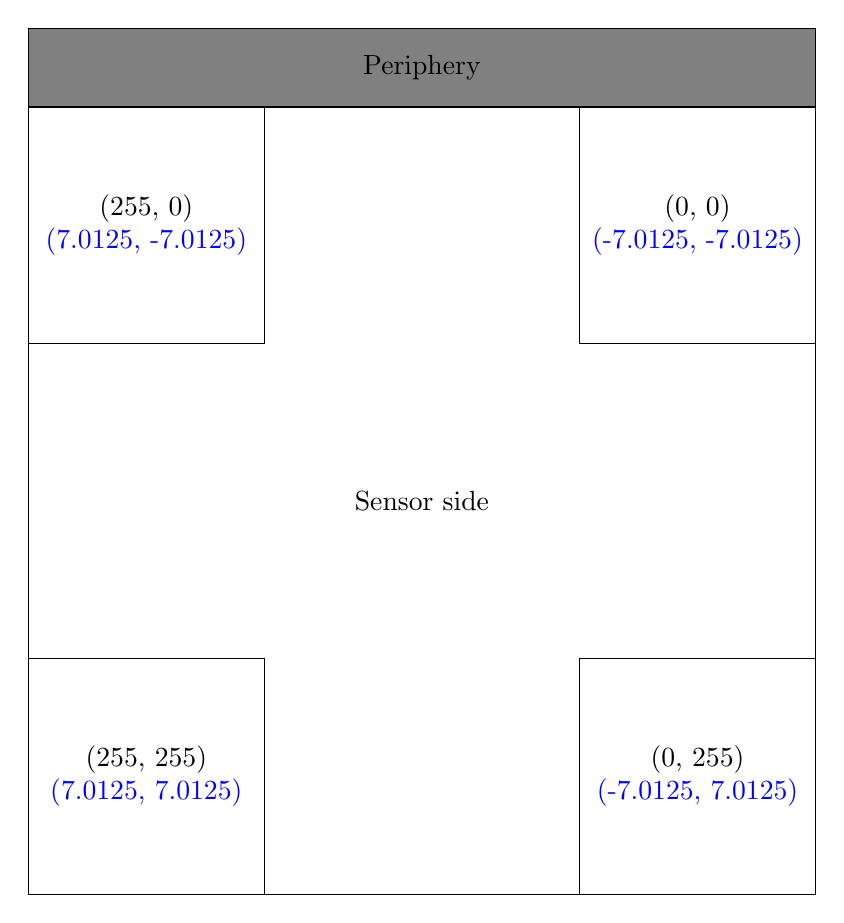
\begin{tikzpicture}
    \begin{scope} 

      \draw (0, 0) rectangle (10, 10) node[pos=.5] {Sensor side};
      \draw[fill=gray] (0, 10) rectangle (10, 11) node[pos=.5]
      {Periphery};

      \draw (0, 10) rectangle (3, 7) node[align=center, pos=.5] {(255, 0) \\ \textcolor{blue}{(7.0125, -7.0125)}};
      \draw (7, 10) rectangle (10, 7) node[align=center, pos=.5] {(0, 0) \\ \textcolor{blue}{(-7.0125, -7.0125)}};
      
      \draw (0, 0) rectangle (3, 3) node[align=center, pos=.5] {(255,
        255) \\ \textcolor{blue}{(7.0125, 7.0125)}};
      \draw (7, 0) rectangle (10, 3) node[align=center, pos=.5] {(0, 255) \\ \textcolor{blue}{(-7.0125, 7.0125)}};
      % \draw[help lines,xstep=.1,ystep=.1] (0, 0) grid (10,10);
      % \foreach \x in {0,1,...,9} { \node [anchor=north] at (\x/10,0) {0.\x}; }
      % \foreach \y in {0,1,...,9} { \node [anchor=east] at (0,\y/10)
      %   {0.\y}; }

    %   \draw[step=2cm,color=gray] (-5, -5) grid (5, 5);
    %   \matrix[matrix of nodes,nodes={inner sep=0pt,text width=2cm,align=center,minimum height=2cm}]{
    %     {(255, 0) \\ \textcolor{blue}{(7.0125, -7.0125)}} & &  & {(0,0) \\ \textcolor{blue}{(-7.0125, -7.0125)}} \\
    %     &  &  &  \\
    %     &  &  &  \\
    %     {(255, 255) \\ \textcolor{blue}{(7.0125, 7.0125)}} &  &  & {(0, 255) \\ \textcolor{blue}{(-7.0125, 7.0125)}} \\};
    \end{scope}  
  \end{tikzpicture}
  \caption{}
  \label{fig:coordinateSystem}
\end{figure}

% ==============================================================================
\chapter{The Timepix3 beam telescope}
\label{ch:Telescope}
% ==============================================================================  

%% --------------------------------------------- %% 

Testing in a high energy beam is a crucial step in the R\&D for the
pixel detector sensors and readout chips. Test beam data are used at
various stages of the development for evaluating the performance of a
prototype in addition to simulations tools like TCAD and
\textsc{Geant4}.

A telescope is used to reconstruct the tracks of the particles going
through its planes. The track position is then extrapolated on the
Device Under Test (DUT). This allows to compare the position of the
hit on the DUT with the reconstructed track and extract the position
and time resolutions as well as the efficiency of the device.

For the CLIC vertex detector R\&D, the Timepix3 telescope is used as a
beam reference. This chapter gives an overview of the components of
the CLICdp Timepix3 telescope and its tracking performance. The
Timepix3 telescope is implemented in AllPix simulations
(c.f. \cref{sec:AllPix}) and its performance is compared to the data
taken at the CERN SPS~\cite{SPS}. Finally, the tracking resolution on
the DUT is extracted in simulations using the Monte Carlo information.

%% --------------------------------------------- %%
\section{Experimental setup at the CERN SPS}
\label{sec:CERN_SPS}
The Timepix3 telescope is placed at the H6 beam~\cite{H6Beamline} of
the CERN SPS typically operated with a $120\,\gev$ pion beam. The
assemblies listed in \cref{tab:Timepix3Assemblies} are tested as DUTs
using this telescope. The beam is configured in such a way to have
$\sim2.6 \times 10^6$ particles per five-second spill. The telescope
planes are positioned in a way to give the best tracking resolution
for the given beam energy taking into account multiple scatterings and
mechanical constraints.
%% --------------------------------------------- %%
\section{Components of the Timepix3 telescope}

%% --------------------------------------------- %%
\subsection{Coordinates system}
A Cartesian right-handed coordinate system is chosen to describe the
geometry of the telescope. The z-direction is along the beam as shown
in \cref{fig:TPX3Telescope} and the y-direction points vertically in
the up direction.

%% --------------------------------------------- %%
\subsection{Sensors and mechanics}
The Timepix3 telescope consists of six planes of Timepix3
ASICs~\cite{Timepix3Poikela} bump bonded to $300\,\micron$ thick
p-in-n planar sensors as shown in \cref{fig:TPX3Telescope}. The planes
are rotated by $9\degrees$ around the x axis (perpendicular to the
beam axis) and the z axis (parallel to the beam axis)
\cite{Akiba:2013yxa}. Given the pixel pitch and the sensor thickness,
this angle mainly leads to clusters of three-hit pixels. Combining the
TOT information, the reconstructed hit position provides sub-pixel
resolution. A tracking resolution of $\sim$$2\,\micron$
on the DUT can be obtained.


\begin{figure}[htbp]
  \centering
  \begin{tikzpicture}
    \node[anchor=south west,inner sep=0] (image) at
    (0,0){\includegraphics[width=0.6\textwidth]{ActiveEdge/Timepix3Telescope.jpeg}};
    \begin{scope}[x={(image.south east)},y={(image.north west)}]
      \node[above, color=white] at (0.5, 0.85) {Device Under Test};
      \node[above, color=white] at (0.5, 0.78) {(\textbf{DUT})};

      \draw[->, very thick, color=black](0.8, 0.25) -- (0.25, 0.25);
      \node[above, color=black] at (0.5, 0.18) {\textbf{Beam}};
      
      %% \draw[help lines,xstep=.1,ystep=.1] (0, 0) grid (1,1);
      %% \foreach \x in {0,1,...,9} { \node [anchor=north] at (\x/10,0) {0.\x}; }
      %% \foreach \y in {0,1,...,9} { \node [anchor=east] at (0,\y/10) {0.\y}; }
      
    \end{scope}
  \end{tikzpicture} 
  \caption{The Timepix3 beam reference telescope with six planes for
    the tracking and the DUT in the middle inserted perpendicular to
    the beam direction.}
  \label{fig:TPX3Telescope}
\end{figure}

The mechanical support for the telescope planes are optimised in order
to reduce the multiple scatterings of the particles and therefore
improving the tracking resolution. The Timepix3 assemblies are mounted
on a PCB as shown in \cref{fig:Timepix3board_PCB}. An aluminum support
is used to hold the PCB which does not cover the sensor. To protect
the sensors from light exposure, an ABS plastic material is used as
cover with a thickness of 2~mm and placed at a distance of 10~mm away
from the PCB (in black in
\cref{fig:TPX3Telescope}). \cref{tab:TPX3TelescopeMaterial} describes
the material (with their thicknesses and radiation lengths) seen by
the particles for each telescope plane which contributes to the
multiple scatterings. The PCB stacks up eight layers of copper
interlacing with Isola IS410 type material with an average fill factor
of $75\%$ for copper. Behind the PCB a layer of Copper is used for the
cooling of the chip. The total material of a telescope plane is
estimated to correspond to $\sim4\%$~X\textsubscript{0}.

\begin{table}[htbp]
  \centering
  \caption{The material in each telescope plane contributing to the
    multiple scatterings of the traversing particles. X refers to the thickness and X\textsubscript{0} to the radiation
    length (both in millimeters).}
  \label{tab:TPX3TelescopeMaterial}
  \begin{tabular}{l c c c}
    \toprule
    Material & X [mm] & X\textsubscript{0} [mm] & X/X\textsubscript{0} [$\%$] \\
    \midrule
    Cooling material for the chip (Cu) & 0.1 & 14.4 & 0.69 \\
    Isola IS410 in the PCB & 1.475 & 167.6 & 0.88 \\
    Copper in the PCB & 0.125 & 14.4 & 0.87 \\
    ASIC (Si) & 0.7 & 93.7 & 0.75\\
    Sensor (Si) & 0.3 & 93.7 & 0.32\\ 
    Sensor cover (ABS plastic) & 2 & 406.4 & 0.49 \\ \hline
    Total & & & 4 \\
    \bottomrule
  \end{tabular}
\end{table}

%% --------------------------------------------- %%
\subsection{Data taking conditions}
The SPIDR readout system, as described in \cref{sec:TimepixReadout},
is used for the data acquisition of the Timepix3 telescope planes. The
Timepix3 readout ASICs are operated with the data-driven
zero-suppressed readout mode. This system allows to record the data
from all the particles from the SPS spill without dead time. The data
is processed offline as described in \cref{sec:recoSoft}.


%% --------------------------------------------- %%
\section{Timepix3 telescope performance}
\label{sec:telescopePerformance}

The Timepix3 telescope is simulated with the \textsc{Geant4}-based
AllPix simulation framework (c.f. \cref{sec:AllPix}). This allows for
a better understanding of the telescope performance, extraction of the
tracking resolution on the DUT and comparison to data. Since AllPix
gives access to the Monte Carlo Truth position (MC position) of the
hits, the true tracking resolution can be obtained by comparing the MC
position with the reconstructed track or hit positions.

\subsection{Timepix3 telescope simulation in AllPix}
In the simulations, the geometry of the telescope is defined as
realistic as possible by taking into account the positions and the
rotations of the telescope planes, the thickness of the sensors and
the pixel pitch. 

The mechanical support for the telescope planes is implemented using
the material as described in \cref{tab:TPX3TelescopeMaterial}.

% \textsc{Geant4} provides the class \textsc{G4Material} which describes
% the macroscopic properties of the material used in simulations and
% contains all the relevant information on its constituent elements. The
% density and the radiation length of the material are the two main
% properties to be considered for the simulations. \textsc{Geant4}
% already provides a material database for all the standard material
% such as copper and silicon. For the Isola IS410, the material
% G4\_BONE\_COMPACT\_ICRU has the closest radiation length and
% density. For the sensor covers in ABS plastic, their constituent
% elements
% (C\textsubscript{8}H\textsubscript{8}~C\textsubscript{4}H\textsubscript{6}~C\textsubscript{3}H\textsubscript{3}N)
% have been implemented as a \textsc{G4Material} in the simulations to
% obtain the correct density and radiation length.

\begin{figure}[htbp]
  \centering
  \begin{tikzpicture}
    \node[anchor=south west,inner sep=0] (image) at
    (0,0){\includegraphics[width=0.6\textwidth]{figures/Telescope/AllpixTelescope.png}};
    \begin{scope}[x={(image.south east)},y={(image.north west)}]
      
      \draw[->, very thick, color=black](0.8, 0.9) -- (0.25, 0.9);
      \node[above, color=black] at (0.5, 0.91) {\textbf{Beam}};
      
      \node[above, color=black] at (0.9, 0.05) {\footnotesize{Plane 0}};
      \node[above, color=black] at (0.75, 0.05) {\footnotesize{Plane 1}};
      \node[above, color=black] at (0.6, 0.05) {\footnotesize{Plane 2}};
      \node[above, color=black] at (0.48, 0.05) {DUT};
      \node[above, color=black] at (0.35, 0.05) {\footnotesize{Plane 3}};
      \node[above, color=black] at (0.2, 0.05) {\footnotesize{Plane 4}};
      \node[above, color=black] at (0.07, 0.05) {\footnotesize{Plane 5}};

      \node[above, color=black] at (0.35, 0.7) {Sensor cover};
      \draw[->, color=black](0.35, 0.7) -- (0.35, 0.45);
      \node[above, color=black] at (0.9, 0.7) {Cooling};
      \draw[->, color=black](0.85, 0.7) -- (0.85, 0.4);

      %% \draw[help lines,xstep=.1,ystep=.1] (0, 0) grid (1,1);
      %% \foreach \x in {0,1,...,9} { \node [anchor=north] at (\x/10,0) {0.\x}; }
      %% \foreach \y in {0,1,...,9} { \node [anchor=east] at (0,\y/10) {0.\y}; }
      
    \end{scope}
  \end{tikzpicture} 
  \caption{The Timepix3 beam reference telescope implemented in AllPix
    with six planes for the tracking and the DUT in the middle
    inserted perpendicular to the beam direction. The sensor covers
    and the chip cooling are shown. The telescope planes numbering
    convention is also shown.}
  \label{fig:Timepix3Telescope_Allpix}
\end{figure}


A digitiser for the Timepix3 readout chips bump-bonded to planar
sensors is defined in AllPix. It simulates the silicon physics by
calculating the diffusion at each \textsc{Geant4} step as described in
\cref{sec:allpix_digitisation}. The contribution of the generated
charge by diffusion in the hit pixel and all its direct neighbouring
pixels is calculated for each step. All the contributions add-up and
the charge in each pixel is calculated. The electronic noise of the
Timepix3 ASIC sums up to the charge in each pixel. Finally a threshold
is applied to each pixel and finally, the pixel-by-pixel TOT
calibration (c.f.~\cref{sec:EnergyCalibration}) is applied.

\textsc{Geant4} General Particle Source (GPS) is used for the
simulation of $120\,\gev$ pions. The GPS generates a parallel beam
with a transverse (radial) standard deviation of 5~mm.

The spread of the tracks used in simulations due to the multiple
scatterings is shown in \cref{fig:MCbeamAngleDistr}. A scattering of
0.1~mrad can cause a displacement of up to $\sim3\,\micron$. The
angles $\phi$ and $\theta$ are given as:

\begin{equation}
  \phi=arctan{{x_2-x_{DUT}} \over {z_2-z_{DUT}}} \; ,
  \label{eq:beamAnglePhi}
\end{equation}

\begin{equation}
  \theta=arctan{{y_2-y_{DUT}} \over {z_2-z_{DUT}}} \; ,
  \label{eq:beamAngleTheta}
\end{equation}

where $x, y$ and $z$ are the MC positions of the hits on the planes 2
and the DUT.

\begin{figure}[htbp] \centering
  \begin{subfigure}[b]{0.45\textwidth}
    \includegraphics[width=\textwidth]{./figures/Telescope/MC_trackAnglePhi_planes_302_50.pdf}
    \caption{}
  \end{subfigure}\hfill
  \begin{subfigure}[b]{0.45\textwidth}
    \includegraphics[width=\textwidth]{./figures/Telescope/MC_trackAngleTheta_planes_302_50.pdf}
    \caption{}
  \end{subfigure}
  \caption{Track angular distribution in \textsc{Geant4} simulations
    comparing the global MC positions on the telescope plane 2 and on
    the DUT.}
  \label{fig:MCbeamAngleDistr}
\end{figure}

The EUTelescope software framework (c.f. \cref{sec:EUTelescope}) is
used to reconstruct the hits on the telescope planes using the
$\eta$-correction method~\cite{Belau:1983eh} and fit the tracks.

%% --------------------------------------------- %%
\subsection{Single-hit resolution on the telescope planes}

\cref{tab:AllPixTelescopePlanesParams} shows the parameters used for
the AllPix simulations of the sensors of the telescope planes. The
bias and the depletion voltages, the sensor type and the threshold
values are the parameters defining the charge sharing and the cluster
size distribution. Therefore they define the intrinsic resolution of
the sensors.

\begin{table}[htbp]
  \centering
  \caption{Parameters used for the simulation of the telescope planes in AllPix.}
  \label{tab:AllPixTelescopePlanesParams}
  \begin{tabular}{cccc}
    \toprule
    Bias voltage [V] & Depletion voltage [V] & Sensor type & Threshold [e-] \\
    \midrule
    50 & 30 & p-in-n & 1000 \\
    \bottomrule
  \end{tabular}
\end{table}


\cref{fig:TelescopeCluSize_data_simu} compares the cluster size
distribution and the charge of the clusters in data and simulations
for the first telescope plane (plane 0). There is a good agreement
between the cluster-size distributions in data and simulations. In
data, there is less single-pixel clusters due to slight imperfections
in the rotations of the planes.

\begin{figure}[htbp] \centering
  \begin{subfigure}[b]{0.3\textwidth}
    \includegraphics[width=\textwidth]{figures/Telescope/biasedResiduals/clusterSizeX_telescope0_data_simu.pdf}
    \caption{}
  \end{subfigure}\hfill
  \begin{subfigure}[b]{0.3\textwidth}
    \includegraphics[width=\textwidth]{figures/Telescope/biasedResiduals/clusterSizeY_telescope0_data_simu.pdf}
    \caption{}
  \end{subfigure}\hfill
  \begin{subfigure}[b]{0.3\textwidth}
    \includegraphics[width=\textwidth]{figures/Telescope/biasedResiduals/clusterSignal_telescope0_data_simu.pdf}
    \caption{}
  \end{subfigure}
  \caption{For the telescope plane 0, the cluster-size distribution in
    the (a) x direction and (b) y direction. (c) shows the sum of the
    charge in the cluster in units of
    TOT.} %data run 661, simulation run 54.
  \label{fig:TelescopeCluSize_data_simu}
\end{figure}

The hit resolution of a telescope plane is given by comparing the
reconstructed hit position with the Monte Carlo Truth position
(x\textsubscript{MC} and y\textsubscript{MC}) obtained by AllPix
simulations. \cref{fig:TelPlane0_MC_hit} shows the hit residuals of
the first telescope plane in x and y directions in simulations which
depend on their thickness, charge sharing and rotations. The standard
deviation of a Gaussian fit on the residuals distributions gives a
resolution of $\sim2.6\,\micron$. Since the residual distribution has
a tail, the RMS of the distribution is $\sim5.8\,\micron$. The
expected resolution of each telescope plane is expected to be
$\sim3.5$. The large tail in the residuals distribution causes the
discrepancy between the expected and the obtained resolution. The tail
in the residuals distribution is due to the reconstruction of the hit
positions of single-pixel clusters where the resolution is defined by
the pixel pitch.

% For this calculation, hits corresponding to tracks with the $10\%$ of
% highest $\chi^2$/NDF are ignored.

\begin{figure}[htbp] \centering
  \begin{subfigure}[b]{0.45\textwidth}
    \includegraphics[width=\textwidth]{figures/Telescope/telescopePlane0_MC_vs_hit_x.pdf}
    \caption{}
  \end{subfigure}\hfill
  \begin{subfigure}[b]{0.45\textwidth}
    \includegraphics[width=\textwidth]{figures/Telescope/telescopePlane0_MC_vs_hit_y.pdf}
    \caption{}
  \end{subfigure}
  \caption{The hit residuals of a telescope plane in (a) x and (b) y
    directions given by comparing the MC and the reconstructed hit
    positions.}
  \label{fig:TelPlane0_MC_hit}
\end{figure}

The residuals as a function of the x\textsubscript{MC} and
y\textsubscript{MC} are shown in \cref{fig:TelPlane0_MC_hit_2D}. The
intrinsic resolution does not depend on the position of the hit. This
confirms the coherence between the geometry description in the AllPix
simulations and the EUTelescope reconstruction. The shape of these
distributions is due to the beam profile which is more focused in the
middle of the sensors.

\begin{figure}[htbp] \centering
  \begin{subfigure}[b]{0.45\textwidth}
    \includegraphics[width=\textwidth]{figures/Telescope/telescopePlane0_MC_vs_hit_x_2D.pdf}
    \caption{}
  \end{subfigure}\hfill
  \begin{subfigure}[b]{0.45\textwidth}
    \includegraphics[width=\textwidth]{figures/Telescope/telescopePlane0_MC_vs_hit_y_2D.pdf}
    \caption{}
  \end{subfigure}
  \caption{The hit residuals of a telescope plane in (a) x and (b) y
    directions comparing the MC and the reconstructed hit positions as
    a function of the MC position.}
  \label{fig:TelPlane0_MC_hit_2D}
\end{figure}


%% --------------------------------------------- %%
\subsection{Biased residuals on each telescope plane}

The tracks on the telescope planes are reconstructed using a
$\chi^2$-minimisation method as described in
\cref{sec:EUTelescope}. The tracks are reconstructed in a biased way
since they include the hit information on each telescope plane. The
biased residual on each telescope plane is defined as the difference
between the measured hit and the biased fitted track position. It
determines the precision with which the track is reconstructed and
depends on the hit resolution of the telescope sensors, the number of
measurements and their positions and finally on the amount of multiple
scattering.

\cref{fig:telescopeBiasedRMS_data_simu} compares the RMS of the biased
residuals in data and simulations (the original distributions are
given in
\cref{fig:telescope_biasedResiduals_data_X,fig:telescope_biasedResiduals_data_Y}
for data and
\cref{fig:telescope_biasedResiduals_simu_X,fig:telescope_biasedResiduals_simu_Y}
for simulation). For this calculation, a cut is applied to discard
$10\%$ of tracks with the highest
$\chi^2$/NDF. \cref{fig:chi2_data_simu} shows the $\chi^2$/NDF
distributions in data (a) and in simulations (b) with the cut on the
$\chi^2$/NDF as illustrated with a red line.

\begin{figure}[htbp] \centering
  \begin{subfigure}[b]{0.45\textwidth}
    \includegraphics[width=\textwidth]{figures/Telescope/biasedResiduals/RMSX_simu_vs_data.pdf}
    \caption{}
  \end{subfigure}\hfill
  \begin{subfigure}[b]{0.45\textwidth}
    \includegraphics[width=\textwidth]{figures/Telescope/biasedResiduals/RMSY_simu_vs_data.pdf}
    \caption{}
  \end{subfigure}
  \caption{The RMS of the biased residuals in the (a) x and (b) y
    directions comparing the data and simulation for the telescope
    planes. A cut is applied to remove $10\%$ of the tracks with the
    highest $\chi^2$/NDF.}
  \label{fig:telescopeBiasedRMS_data_simu}
\end{figure}


\begin{figure}[htbp] \centering
  \begin{subfigure}[b]{0.45\textwidth}
    \includegraphics[width=\textwidth]{figures/Telescope/biasedResiduals/chi2_run661.pdf}
    \caption{Data}
  \end{subfigure}\hfill
  \begin{subfigure}[b]{0.45\textwidth}
    \includegraphics[width=\textwidth]{figures/Telescope/biasedResiduals/chi2_run77.pdf}
    \caption{Simulation}
  \end{subfigure}
  \caption{$\chi^2$/NDF distributions for (a) data and (b)
    simulation. A cut is applied to remove the $10\%$ of tracks with
    highest $\chi^2$/NDF (illustrated with the red line).}
  \label{fig:chi2_data_simu}
\end{figure}

The simulation is in good agreement with data in terms of biased
residuals. This means that the hit resolution of the telescope planes
and the amount of the multiple scatterings in the simulation are close
to reality and the simulation can be used to get a good estimation of
the tracking resolution on the DUT.

The width of the biased residuals increases with the distance (in z
direction). In fact, the uncertainty on the deflection angle due to
the multiple scatterings increases with larger distances of the
telescope planes.



\subsection{Tracking resolution on the DUT}
The tracking residuals on the DUT in the x and y directions is shown
in \cref{fig:DUT_MC_track}. This value can be only obtained in
simulations as the MC position is needed. For this calculation, the
same cut on the $\chi^2$/NDF as shown in \cref{fig:chi2_data_simu} is
applied for the track selection.

\begin{figure}[htbp] \centering
  \begin{subfigure}[b]{0.45\textwidth}
    \includegraphics[width=\textwidth]{figures/Telescope/Unbiased_trackRes_DUT_x.pdf}
    \caption{}
  \end{subfigure}\hfill
  \begin{subfigure}[b]{0.45\textwidth}
    \includegraphics[width=\textwidth]{figures/Telescope/Unbiased_trackRes_DUT_y.pdf}
    \caption{}
  \end{subfigure}
  \caption{The track residuals on the DUT comparing the reconstructed
    track position to the true position of the particles obtained from
    \textsc{Geant4} in AllPix simulations in (a) x and (b) y
    directions.}
  \label{fig:DUT_MC_track}
\end{figure}


The tracking resolution on the DUT as a function of the
x\textsubscript{MC} and y\textsubscript{MC} positions is shown in
\cref{fig:DUT_MC_track_2D}. In the y-direction, the residuals show a
shift of $\sim1\,\micron$. This can be explained to the fact that in
the y-direction, the three planes before the DUT are rotated in an
asymmetric way compared to the three other planes after the DUT in the
Timepix3 telescope. 

The standard deviation of the distributions is less than $2\,\micron$
which allows for in-pixel studies.

\begin{figure}[htbp] \centering
  \begin{subfigure}[b]{0.45\textwidth}
    \includegraphics[width=\textwidth]{figures/Telescope/Unbiased_trackRes_DUT_x_2D.pdf}
    \caption{}
  \end{subfigure}\hfill
  \begin{subfigure}[b]{0.45\textwidth}
    \includegraphics[width=\textwidth]{figures/Telescope/Unbiased_trackRes_DUT_y_2D.pdf}
    \caption{}
  \end{subfigure}
  \caption{The tracking resolution on the DUT in (a) x and (b)
    directions as a function of the MC position.}
  \label{fig:DUT_MC_track_2D}
\end{figure}




%% --------------------------------------------- %%
\cref{tab:SummaryOfResolutions} summarises the telescope performance
obtained in the simulations. The simulations confirm that the Timepix3
telescope allows for a high resolution track reconstruction on the DUT
($\sim2\,\micron$) as expected by~\cite{Akiba:2013yxa}. This telescope
is adapted for in-pixel studies and testing the DUTs with high
resolution constraints as expected for CLIC.

In \cref{ch:ThinSensorsStudies} the Timepix3 telescope is used to
precisely measure the resolution of thin sensors.

\begin{table}[htbp]
  \centering
  \caption{A summary of the measured telescope performance.}
  \label{tab:SummaryOfResolutions}
  \begin{tabular}{ccc}
    \toprule
    $\sigma$\textsubscript{int} [$\micron$] & $\sigma$\textsubscript{x,DUT} [$\micron$] & $\sigma$\textsubscript{y,DUT} [$\micron$]\\
    \midrule
    2.6 & 1.94 & 1.80 \\
    \bottomrule
  \end{tabular}
\end{table}
% ==============================================================================
\chapter{Thin sensors studies}
\label{ch:ThinSensorsStudies}
% ==============================================================================    

% The aim of the CLIC vertex detector is the precise determination of
% the displaced vertices and jet flavour-tagging in an environment with
% high occupancy from beam-induced backgrounds. Multi-layer barrel and
% endcap pixel detectors with geometrical coverage extending down to low
% polar angles ($\theta_{min}\sim8^{\circ}$) are foreseen to fulfill
% these requirements. The goal is to achieve a single-point resolution
% of $\sim 3\,\micron$ with $25\,\micron$ pixel pitch and analogue
% readout. A material budget of $\sim0.2\%$~X\textsubscript{0} per layer
% is required including readout, support and cabling. This can be
% achieved with $50\,\micron$ thick sensors on $50\,\micron$ thick
% readout ASICs.

As part of the R\&D programme for the CLIC vertex detector, the
performance of thin silicon sensors is quantified using the Timepix3
readout chip with $55\,\micron$ pixel pitch. $50\,\micron$ to
$150\,\micron$ thick planar sensors are bump-bonded to $750\,\micron$
thick Timepix3 ASICs. These assemblies are tested in test beams using
the CLICdp Timepix3 telescope.

The AllPix simulation framework (described in \cref{sec:AllPix}) is
used to simulate the performance of thin sensors and to understand the
charge sharing in such sensors. For the DUT the same digitiser as for
the Timepix3 telescope planes is used
(c.f. \cref{sec:allpix_digitisation}). This digitiser takes into
account the semiconductor physics, drift, diffusion charge sharing in
the planar sensors and also noise in the readout ASICs. The data is
used to validate the simulations. The simulation is finally
extrapolated for smaller pixels of $25\,\micron$ pitch.

%% --------------------------------------------- %%
\section{Thin-sensor assemblies}
A summary of thin sensors ($50-150\,\micron$ thick) bump-bonded to the
CLICdp Timepix3 readout ASICs is shown in
\cref{tab:Timepix3Assemblies}. These assemblies are tested using the
Timepix3 pixel beam reference telescope at the CERN SPS with the
experimental setup as described in \cref{sec:CERN_SPS}.

%% --------------------------------------------- %%
\subsection{Operating conditions}
\label{sec:operatingConditions}
The Timepix3 readout ASICs were operated with the optimised parameters
as described in \cref{tab:timepix3Operation}. The nominal values for
the threshold and the bias voltage are shown in
\cref{tab:nominalBiasThreshold}. For the nominal bias voltage, the
sensor is fully (or over) depleted. The nominal threshold set insures
that the readout chip is not operating in noisy
conditions. \cref{sec:noise} describes the procedure for the selection
of the nominal threshold value. These nominal values are held
throughout the data taking except for the cases where the threshold or
the bias voltages are scanned.

\begin{table}[htbp]
  \centering
  \caption{Nominal operating bias voltage, threshold in DAC and
    calibrated in number of electrons (measured as described in
    \cref{sec:thresholdCalibration}) for the tested assemblies as
    shown in \cref{tab:Timepix3Assemblies}.}
  \label{tab:nominalBiasThreshold}
  \begin{tabular}{lcccc}
    \toprule
    Timepix3 ID & Thickness [$\micron$] & Bias voltage [V] & Threshold [DAC] & Threshold [e\textsuperscript{-}]\\
    \midrule
    W19\_G7 & 50 & -15 & 1190 & $526.2\pm0.7$ \\
    W19\_F7 & 50 & -15 & 1187 & $600.4\pm0.6$ \\
    W19\_L8 & 50 & -15 & 1133 & $568.5\pm0.5$ \\
    W19\_C7 & 50 & -15 & 1148 & $608.7\pm0.5$ \\ \hline
    W5\_E2 & 100 & -20 & 1160 & $561.0\pm0.7$ \\ \hline
    W5\_F1 & 150 & -30 & 1153 & $554.9\pm0.5$ \\ %%\hline
    %% W2\_J5 & 300 & 100 & 1170 & $565.7\pm1.6$ \\
    \bottomrule
  \end{tabular}
\end{table}

% %% --------------------------------------------- %%
% \section{Samples and sensors geometries}
% %% The DAC settings used for the operation of the Timepix3 assemblies in
% %% test beams is summarised in \cref{tab:timepix3Operation}.
% %% \begin{itemize}
% %% \item I\textsubscript{krum} DAC is set to 10.
% %% \item TOT clock frequency: $40\,\megahertz$
% %% \item VFBK: 150
% %% \end{itemize}


% For most of the measurements, the DUT is perpendicular to the beam. A
% scan was done on the bias voltage and the threshold of the DUT. The
% bias scan allows to obtain the depletion voltage.

%% --------------------------------------------- %%
\section{Calibrated test beam data}

The test pulse calibration as described in
\cref{sec:EnergyCalibration} is applied to the test beam data in order
to convert the TOT values into energy deposited (in electrons) by the
MIP particles.


\cref{sec:testBeamDataCalibrated_TOT} shows the TOT distribution for
one, two, three and four-pixel clusters. The MPV of the TOT
distributions for different cluster sizes do not align due to the
non-linear behaviour of the Timepix3, as sharing the same deposited
charge amongst several pixels results in each pixel having a higher
TOT than would be expected from simply scaling the charge. The
calibrated energy distribution aligns for different cluster sizes
since the calibration takes into account the non-linearities of the
chip as shown in \cref{sec:testBeamDataCalibrated_Edep}. For the
$50\,\micron$ thick sensor, the calibrated distributions do not align
since higher deposited energies tend to give higher cluster sizes and
the distributions for larger cluster sizes are biased towards larger
energy depositions.

\begin{figure}[htbp] \centering
  \begin{subfigure}[b]{0.3\textwidth}
    \includegraphics[width=\textwidth]{./figures/Calibration/TOT_Clusters_W0019_C07.pdf}
    \caption{W19\_C7}
  \end{subfigure} \hfill
  \begin{subfigure}[b]{0.3\textwidth}
    \includegraphics[width=\textwidth]{./figures/Calibration/TOT_Clusters_W0005_E02.pdf}
    \caption{W5\_E2}
  \end{subfigure}\hfill
  \begin{subfigure}[b]{0.3\textwidth}
    \includegraphics[width=\textwidth]{./figures/Calibration/TOT_Clusters_W0005_F01.pdf}
    \caption{W5\_F1}
  \end{subfigure}
  \caption{TOT distribution for one, two, three and four-pixel
    clusters for various assemblies with (a) $50\,\micron$, (b)
    $100\,\micron$ and (c) $150\,\micron$ thick planar sensors.}
  \label{sec:testBeamDataCalibrated_TOT}
\end{figure}

\begin{figure}[htbp] \centering
  \begin{subfigure}[b]{0.33\textwidth}
    \includegraphics[width=\textwidth]{./figures/Calibration/Edep_Clusters_W0019_C07.pdf}
    \caption{W19\_C7}
  \end{subfigure} \hfill
  \begin{subfigure}[b]{0.33\textwidth}
    \includegraphics[width=\textwidth]{./figures/Calibration/Edep_Clusters_W0005_E02.pdf}
    \caption{W5\_E2}
  \end{subfigure}\hfill
  \begin{subfigure}[b]{0.33\textwidth}
    \includegraphics[width=\textwidth]{./figures/Calibration/Edep_Clusters_W0005_F01.pdf}
    \caption{W5\_F1}
  \end{subfigure}
  \caption{Energy deposition distribution for one, two, three and
    four-pixel clusters for various assemblies with (a) $50\,\micron$,
    (b) $100\,\micron$ and (c) $150\,\micron$ thick planar sensors.}
  \label{sec:testBeamDataCalibrated_Edep}
\end{figure}

For all assemblies, the energy deposition in electrons is given in
\cref{sec:appendixCalibDataG4}.

\cref{fig:G4_simu_data_Edep} compares the total energy deposition in a
cluster in data and simulation. The most-probable-value (MPV) and the
width of the distributions in data and simulation agree. Therefore the
calibration is validated.

\begin{figure}[htbp] \centering
  \begin{subfigure}[b]{0.3\textwidth}
    \includegraphics[width=\textwidth]{figures/TestBeam/50micron_Edep.pdf}
    \caption{$50\,\micron$}
  \end{subfigure} \hfill
  \begin{subfigure}[b]{0.3\textwidth}
    \includegraphics[width=\textwidth]{figures/TestBeam/100micron_Edep.pdf}
    \caption{$100\,\micron$}
  \end{subfigure} \hfill
  \begin{subfigure}[b]{0.3\textwidth}
    \includegraphics[width=\textwidth]{figures/TestBeam/150micron_Edep.pdf}
    \caption{$150\,\micron$}
  \end{subfigure} 
  %% \hfill
  %% \begin{subfigure}[b]{0.23\textwidth}

  %%   \caption{$300\,\micron$}
  %% \end{subfigure}
  \caption{The energy deposition for all cluster sizes in simulation
    and data for (a) W19\_G7, (b) W5\_E2 and (c) W5\_F1. The
    assemblies are operated at nominal conditions.}
  \label{fig:G4_simu_data_Edep}
\end{figure}


%% --------------------------------------------- %%
\section{Experimental and simulated results for thin sensors}

This section gives an overview on the performance of thin sensors and
compares data with AllPix simulations.

%% --------------------------------------------- %%
\subsection{Measurement of the depletion voltage}
\label{sec:ThinSensors_depletionVoltage}

The depletion voltage corresponds to the voltage at which the sensor
is fully depleted and the charge of the full thickness of the sensor
is collected. This can be measured in test beams by scanning the bias
voltage. For lower bias voltages the sensor is under depleted and
therefore the collected charge is also reduced. The depletion voltage
and the sensor thickness are related by \cref{eq:depletionVoltage}.

To obtain the depletion voltage, the total measured TOT is calculated
by summing up the TOT in the clusters considering all cluster
sizes. The distribution is fitted with a landau function convoluted
with a Gaussian. The fit is done using RooFit~\cite{Cranmer:2012sba}
and an example is given in \cref{fig:W5_F1_DepletionVoltage_TOTdistr}.
\cref{fig:W2_J5_DepletionVoltage_chargeVSbiasVoltage} shows the most
probable value (MPV) of the measured TOT as a function of the square
root of the bias voltage. The TOT MPV shows two distinct regions: a
sloped region and a plateau region. The depletion voltage of the
assembly is obtained by calculating the intersection of a linear fit
performed on both regions (defined by eye). The calculated depletion
voltages for all assemblies is summarised in
\cref{tab:depletionVoltage,fig:depletionVoltage}. The $50\,\micron$
thick sensor is depleted at a low bias voltage of $\sim$2~V. However
the measurement was done with a bias step size of $1$~V and the fits
give a higher depletion voltage of $\sim7$~V. From the depletion
voltage, the concentration of the dopants in the bulk is calculated to
be around $N_{bulk}\approx1.3\,\inversemetercubic$ and corresponds to
a resistivity of $\rho\approx10\text{k}\Omega\text{cm}$ for all the
assemblies.

\begin{figure}[htbp]\centering
  \begin{subfigure}[b]{0.45\textwidth}
  \includegraphics[width=\textwidth]{./figures/TestBeam/W5_F1_totalTOT_Langau_run761.pdf}
  % W2_J5_totalTOT_Langau_run1998.pdf}
  \caption{}\label{fig:W5_F1_DepletionVoltage_TOTdistr}
  \end{subfigure} \hfill
  \begin{subfigure}[b]{0.45\textwidth}
    \includegraphics[width=\textwidth]{./figures/TestBeam/depletionVoltage_W0005_F01_Edep.pdf}
    \caption{}\label{fig:W2_J5_DepletionVoltage_chargeVSbiasVoltage}
  \end{subfigure}
  \caption{(a) The measured energy deposition distribution in a
    $150\,\micron$ thick silicon sensor (W5\_F1) with a bias voltage
    of -30~V fitted with a Landau function convoluted with a Gaussian
    function. (b) The most probable value of the measured energy
    deposition as a function of the bias voltage for W5\_F1. Straight
    lines are used to fit the slope and the plateau regions. The
    depletion voltage corresponds to the intersection of these two
    regions and shown in a red dashed line. The continuous red line
    shows the nominal operating bias voltage.}
  \label{fig:W5_F1_DepletionVoltage}
\end{figure}

\begin{table}[htbp]
  \centering
  \caption{Measured depletion voltage for the assemblies described in
    \cref{tab:Timepix3Assemblies} and calculated by fitting the
    plateau and slope regions of TOT as a function of the bias
    voltage.}
  \label{tab:depletionVoltage}
  \begin{tabular}{lc}
    \toprule
    Assembly & Depletion voltage [V] \\
    \midrule
    W19\_G7 & -7 \\
    W19\_F7 & -7\\
    W19\_L8 & -7\\
    W19\_C7 & -7\\ \hline
    W5\_E2 & -12 \\ \hline
    W5\_F1 & -15 \\ %\hline
%    W2\_J5 & 63.23 \\ 
    \bottomrule
  \end{tabular}
\end{table}

%% --------------------------------------------- %%
\subsection{Cluster size distribution}
The cluster size distribution is an indication on the amount of charge
sharing in a sensor. For thicker sensors, more charge sharing is
expected since the charge drifts in a longer distance and diffuses
across a larger transverse area. The threshold of the readout
electronics has a large impact on the detection of the charge
sharing. The threshold should be as low as possible to avoid
undetected energy deposits.

In this analysis, the hit pixels form a cluster with a distance
criterion of $\sqrt{2}$: pixels sharing common corners or edges are
considered as clusters. For sensor thicknesses in the range of
$50\,\micron$-$150\,\micron$, clusters of size one to four are
expected due to the charge sharing. Larger clusters are expected due
to other effects such as $\delta$-rays.

The most common cluster shapes are illustrated in
\cref{tab:clusizeShapes}.

\begin{table}
  \centering
  \caption{Most common cluster shapes.}
  \label{tab:clusizeShapes}
  \begin{tabular}{ccccc}
    \toprule
    Shape & Cluster size & Size in $x$ & Size in $y$ & Name \\
    \midrule
    \begin{tikzpicture}
      \draw (0,0) rectangle (0.5,-0.5);
    \end{tikzpicture}
    & 1 & 1 & 1 & size 1 ($1\times1$) \\
    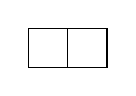
\begin{tikzpicture}
      \draw (0.0,0.0) rectangle (0.5,-0.5);
      \draw (0.5,0.0) rectangle (1.0,-0.5);
    \end{tikzpicture}
    & 2 & 2 & 1 & size 2 ($2\times1$) \\
    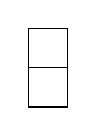
\begin{tikzpicture}
      \draw (0.0,0.0) rectangle (0.5,-0.5);
      \draw (0.0,0.5) rectangle (0.5,0.0);
    \end{tikzpicture}
    & 2 & 1 & 2 & size 2 ($1\times2$) \\
    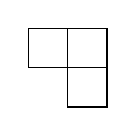
\begin{tikzpicture}
      \draw (0.0,0.0) rectangle (0.5,-0.5);
      \draw (0.5,-0.5) rectangle (1.0,-1.0);
      \draw (0.5,0.0) rectangle (1.0,-0.5);
    \end{tikzpicture}
    & 3 & 2 & 2 & size 3 ($2\times2$)\\
    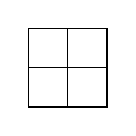
\begin{tikzpicture}
      \draw (0.0,0.0) rectangle (0.5,-0.5);
      \draw (0.5,-0.5) rectangle (1.0,-1.0);
      \draw (0.5,0.0) rectangle (1.0,-0.5);
      \draw (0.0,-0.5) rectangle (0.5,-1.0);
    \end{tikzpicture}
    & 4 & 2 & 2 & size 4 ($2\times2$) \\
    \bottomrule
  \end{tabular}
\end{table}

\cref{fig:G4_simu_data_cluSize} compares the cluster-size distribution
in simulations and data for the assemblies operated at nominal
conditions. There is a good agreement between simulation and data in
terms of cluster-size distribution.

\begin{figure}[htbp] \centering
  \begin{subfigure}[b]{0.3\textwidth}
    \includegraphics[width=\textwidth]{figures/TestBeam/50micron_sizeX.pdf}
    \caption{$50\,\micron$ (W19\_G7)}
  \end{subfigure} \hfill
  \begin{subfigure}[b]{0.3\textwidth}
    \includegraphics[width=\textwidth]{figures/TestBeam/100micron_sizeX.pdf}
    \caption{$100\,\micron$ (W5\_E2)}
  \end{subfigure} \hfill
  \begin{subfigure}[b]{0.3\textwidth}
    \includegraphics[width=\textwidth]{figures/TestBeam/150micron_sizeX.pdf}
    \caption{$150\,\micron$ (W5\_F1)}
  \end{subfigure} 
  %% \hfill
  %% \begin{subfigure}[b]{0.23\textwidth}

  %%   \caption{$300\,\micron$ p-in-n}
  %% \end{subfigure}
  \caption{The cluster size distribution in simulation and data for
    $50\,\micron$, $100\,\micron$ and $150\,\micron$ thick
    sensors. The assemblies are operated at nominal conditions.}
  \label{fig:G4_simu_data_cluSize}
\end{figure}


The fraction of different cluster sizes depends on the operating
conditions of the assemblies like the bias voltage and the threshold
of the readout ASICs. \cref{fig:cluSize_operatingConditions} shows the
cluster size fraction for a $150\,\micron$ thick sensor (assembly
W5\_F1) operated at different bias voltages and thresholds.  

Higher bias voltages reduce the amount of charge sharing since the
drift time is lowered in a stronger electric field and the charges
diffuse less in the transverse direction. For very low bias voltages,
the sensor is under-depleted. An increase in bias voltage in this
regime increases the charge sharing. The pixel neighbouring a hit
pixel is more likely to be over threshold as more charge is
collected. The results for other assemblies are shown in
\cref{fig:clusterSize_vs_biasVoltage}.

Lowering the threshold leads to an increase in the average cluster
size fraction distribution. Results for all assemblies are shown in
\cref{fig:clusterSize_vs_THLscan}.


\begin{figure}[htbp] \centering
  \begin{subfigure}[b]{0.45\textwidth}
    \includegraphics[width=\textwidth]{./figures/TestBeam/cluSize_biasScan_W0005_F01.pdf}
    \caption{}
  \end{subfigure} \hfill
  \begin{subfigure}[b]{0.45\textwidth}
    \includegraphics[width=\textwidth]{./figures/TestBeam/cluSize_THLscan_W0005_F01.pdf}
    \caption{}
  \end{subfigure}
  \caption{Cluster-size distribution as a function of (a) bias voltage
    and (b) threshold for the assembly W5\_F1 with a $150\,\micron$
    thick sensor.}
  \label{fig:cluSize_operatingConditions}
\end{figure}


The cluster size fraction as a function of the sensor thickness for
data recorded at the nominal operating conditions is shown in
\cref{fig:cluSize_thickness}. Charge sharing increases with sensor
thickness. The fraction of $1\times2$ and $2\times1$-pixel clusters
are very similar for square pixels and the curve labeled 2-pixel
clusters combine these two cluster geometries.

\begin{figure}[htbp] 
  \centering
  \includegraphics[width=0.5\textwidth]{./figures/TestBeam/cluSize_vs_thickness.pdf}
  \caption{Cluster-size distribution as a function of sensor thickness
    for runs recorded under nominal operating conditions.}
  \label{fig:cluSize_thickness}
\end{figure}

%% --------------------------------------------- %%
\subsection{Charge sharing as a function of the track position}

The charge sharing is studied by extrapolating the track position
obtained from the Timepix3 telescope to the DUT. The size of the
clusters depends on the track position within the pixel. For
perpendicular tracks, multi-pixel clusters are created when the track
hits the edges or the corners of a pixel, leading to the charge
sharing between the pixel and its neighbouring pixels. The charge
sharing is also affected by the operating threshold of the readout
ASIC. \cref{fig:chargeSharingTrack} illustrates the track position
within the pixel for 1 to 4-pixel cluster sizes for a $50\,\micron$
sensor. For other thicknesses, the track position within the pixel is
shown in
\cref{fig:chargeSharingTrack_W19_G7,fig:chargeSharingTrack_W5_E2,fig:chargeSharingTrack_W5_F1}.

\begin{figure}[htbp] \centering
  \begin{subfigure}[b]{0.23\textwidth}
    \includegraphics[width=\textwidth]{./figures/TestBeam/TrackPosWPixel_1hit_runW19_G7.pdf}
    \caption{Cluster size 1}
  \end{subfigure} \hfill
  \begin{subfigure}[b]{0.23\textwidth}
    \includegraphics[width=\textwidth]{./figures/TestBeam/TrackPosWPixel_2hit_runW19_G7.pdf}
    \caption{Cluster size 2}
  \end{subfigure} \hfill
  \begin{subfigure}[b]{0.23\textwidth}
    \includegraphics[width=\textwidth]{./figures/TestBeam/TrackPosWPixel_3hit_runW19_G7.pdf}
    \caption{Cluster size 3}
  \end{subfigure} \hfill
  \begin{subfigure}[b]{0.23\textwidth}
    \includegraphics[width=\textwidth]{./figures/TestBeam/TrackPosWPixel_4hit_runW19_G7.pdf}
    \caption{Cluster size 4}
  \end{subfigure}
  \caption{Extrapolated track position within the pixel for 1 to
    4-pixel cluster sizes for a $50\,\micron$ sensor (assembly
    W19\_G7). The assembly is operated at nominal conditions.}
  \label{fig:chargeSharingTrack}
\end{figure}

\cref{fig:chargeSharing_2PC} compares the track position within the
pixel for two-pixel clusters in a one-dimensional profile for
different sensor thicknesses. For thinner sensors, the track position
should be closer to the edges of the pixels to create two-pixel
clusters.

\begin{figure}[htbp] 
  \centering
  \includegraphics[width=0.5\textwidth]{./figures/TestBeam/chargeSharing_2pixel_clusters.pdf}
  \caption{Track position within the pixel for tracks leading to
    two-pixel clusters for different sensor thicknesses (the
    histograms are scaled to have a unit area).}
  \label{fig:chargeSharing_2PC}
\end{figure}


\subsection{Single-point resolution}

From the test-beam data, the residuals are calculated by comparing the
reconstructed hit position with the extrapolated track position
obtained by the telescope. This residual combines in quadrature the
single-point (or hit) and the track resolutions:

\begin{equation}
  \sigma_{\mathrm{residual}}^{2}=\sigma_{\mathrm{hit}}^{2}+\sigma_{\mathrm{track}}^{2} .
  \label{eq:residualEq}
\end{equation}

In the following, the tracking resolution of $\sim2\,\micron$ is not
unfolded from the residual measurements presented. 
% For the estimation
% of the single-point resolution, the tracking resolution of
% $\sim2\,\micron$ at the SPS test beam should be unfolded
% (c.f.~\cref{ch:Telescope}).

The residuals depend highly on the cluster sizes since the
reconstructed hit position takes into account the number of the hit
pixels in a cluster and the charge information in each
pixel. \cref{fig:residuals_cluSize} illustrates the residuals for a
$50\,\micron$ thick sensor (assembly W19\_G7) for different cluster
sizes. For single-pixel clusters, the hit position corresponds to the
geometric center of the pixel and therefore a resolution of
pitch$/\sqrt{12}$ is expected (as explained in
\cref{sec:binaryReadout}). For multi-pixel clusters, by using the
charge information, a more accurate interpolation of the hit position
can be obtained and the resolution is better than the geometrical
information (by using the $\eta$-correction method as described in
\cref{sec:EtaCorrection}).

\begin{figure}[htbp] \centering
  \begin{subfigure}[b]{0.23\textwidth}
    \includegraphics[width=\textwidth]{./figures/TestBeam/residual_1hit_W19_G7.pdf}
    \caption{Cluster size 1}
  \end{subfigure} \hfill
  \begin{subfigure}[b]{0.23\textwidth}
    \includegraphics[width=\textwidth]{./figures/TestBeam/residual_2hit_W19_G7.pdf}
    \caption{Cluster size 2}
  \end{subfigure} \hfill
  \begin{subfigure}[b]{0.23\textwidth}
    \includegraphics[width=\textwidth]{./figures/TestBeam/residual_3hit_W19_G7.pdf}
    \caption{Cluster size 3}
  \end{subfigure} \hfill
  \begin{subfigure}[b]{0.23\textwidth}
    \includegraphics[width=\textwidth]{./figures/TestBeam/residual_4hit_W19_G7.pdf}
    \caption{Cluster size 4}
  \end{subfigure}
  \caption{The residuals for a $50\,\micron$ thick sensor (assembly
    W19\_G7) for different cluster sizes: (a) Cluster size 1
    ($1\times1$), (b) Cluster size 2 ($2\times1$), (c) Cluster size 3
    ($2\times2$) and (d) Cluster size 4 ($2\times2$). The track
    resolution of $\sim2\,\micron$ is not unfolded.}
  \label{fig:residuals_cluSize}
\end{figure}

The overall residual is defined by the RMS of the residual of all
tracks combined. The distribution of the residuals for different
sensor thicknesses operated at nominal conditions in simulation and
data is shown in \cref{fig:G4_simu_data_Residuals}. The wider
component in the residual distributions corresponds to the
single-pixel clusters. For thicker sensors, the fraction of
multi-pixel clusters increases. This leads to a higher fraction of
more precisely reconstructed hits and therefore the residual
distribution gets narrower. There is a good agreement between
simulation and data in terms of the residuals distribution.

\begin{figure}[htbp] \centering
  \begin{subfigure}[b]{0.3\textwidth}
    \includegraphics[width=\textwidth]{figures/TestBeam/50micron_resX.pdf}
    \caption{$50\,\micron$}
  \end{subfigure} \hfill
  \begin{subfigure}[b]{0.3\textwidth}
    \includegraphics[width=\textwidth]{figures/TestBeam/100micron_resX.pdf}
    \caption{$100\,\micron$}
  \end{subfigure} \hfill
  \begin{subfigure}[b]{0.3\textwidth}
    \includegraphics[width=\textwidth]{figures/TestBeam/150micron_resX.pdf}
    \caption{$150\,\micron$}
  \end{subfigure} 
  %% \hfill
  %% \begin{subfigure}[b]{0.23\textwidth}

  %%   \caption{$300\,\micron$ p-in-n}
  %% \end{subfigure}
  \caption{The residuals distribution in the x direction in simulation
    and data for the assemblies (a) W19\_G7, (b) W5\_E2 and (c)
    W5\_F1. The assemblies are operated at nominal conditions. The
    track resolution is not unfolded.}
  \label{fig:G4_simu_data_Residuals}
\end{figure}

%% \begin{figure}[htbp] \centering
%%   \begin{subfigure}[b]{0.23\textwidth}
%%     \includegraphics[width=\textwidth]{./figures/TestBeam/residualsHist_W19_C7.pdf}
%%     \caption{$50\,\micron$ sensor}
%%   \end{subfigure} \hfill
%%   \begin{subfigure}[b]{0.23\textwidth}
%%     \includegraphics[width=\textwidth]{./figures/TestBeam/residualsHist_W5_E2.pdf}
%%     \caption{$100\,\micron$ sensor}
%%   \end{subfigure} \hfill
%%   \begin{subfigure}[b]{0.23\textwidth}
%%     \includegraphics[width=\textwidth]{./figures/TestBeam/residualsHist_W5_F1.pdf}
%%     \caption{$150\,\micron$ sensor}
%%   \end{subfigure} \hfill
%%   \begin{subfigure}[b]{0.23\textwidth}

%%     \caption{$300\,\micron$ sensor}
%%   \end{subfigure}
%%   \caption{Examples of the residuals distributions in the x direction
%%     for the assemblies (a) W19\_C7, (b) W5\_E2 and (c) W5\_F1. The
%%     track resolution is not unfolded.}
%%   \label{fig:residualsHist_thickness}
%% \end{figure}


The factors affecting the fraction of different cluster sizes such as
the sensor thickness and the operating conditions of the assembly
(threshold and bias voltage) affect as well the
residuals. \cref{fig:Residuals_bias_threshold} shows the RMS of the
residuals in the x and y directions for a $50\,\micron$ thick sensor
(assembly W19\_G7) as a function of the bias voltage and the
threshold. For other assemblies, these plots are shown in
\cref{fig:Residuals_vs_biasVoltage,fig:Residuals_vs_Threshold}. The
residuals follow the same trend as the cluster size distributions:
higher fractions of single-pixel clusters result in larger residuals.


\begin{figure}[htbp] \centering
  \begin{subfigure}[b]{0.45\textwidth}
    \includegraphics[width=\textwidth]{./figures/TestBeam/W19_G7_Residual_vs_bias.pdf}
    \caption{}
  \end{subfigure} \hfill
  \begin{subfigure}[b]{0.45\textwidth}
    \includegraphics[width=\textwidth]{./figures/TestBeam/residuals_W0019_G07_THLscan.pdf}
    \caption{}
  \end{subfigure}
  \caption{The RMS of the residuals in x and y directions as a
    function of (a) bias voltage and (b) threshold for a $50\,\micron$
    thick sensor (assembly W19\_G7). The track resolution of
    $\sim2\,\micron$ is not unfolded.}
  \label{fig:Residuals_bias_threshold}
\end{figure}


For the assemblies operated at the nominal operating conditions, the
RMS of the residuals in the x and y directions as a function of the
sensor thickness are shown in \cref{fig:residuals_thickness}. For
thicker sensors the fraction of multi-pixel clusters is higher and
results in lower residuals. 

\begin{figure}[htbp] 
  \centering
  \includegraphics[width=0.5\textwidth]{./figures/TestBeam/residuals_vs_thickness.pdf}
  \caption{The RMS of the residuals in x and y directions as a
    function of the sensor thickness for assemblies operated at the
    nominal condition. The track resolution is not unfolded.}
  \label{fig:residuals_thickness}
\end{figure}



%% --------------------------------------------- %%
\subsection{Global detection efficiency}

The detection efficiency of the assemblies is defined as the fraction
of total number of hits matched to tracks (within a window of radius
0.1~mm) and the total number of tracks projected to pass through the
assembly. The efficiency is calculated within the matrix of
$256\times256$ pixels of the main sensor area and the hot or masked
pixels are not excluded from this calculation. They contribute to the
assemblies' inefficiencies.

The detection efficiency is strongly related to the operating
threshold of the readout ASIC. With a lower threshold, smaller energy
depositions can be measured and it is more likely to detect a
particle. \cref{fig:efficiency_VS_Threshold} shows the detection
efficiency for different sensor thicknesses. For thinner sensors, the
energy deposition is lower and the efficiency drops more quickly by
increasing the threshold than for thick sensors.

\begin{figure}[htbp] 
  \centering
  \begin{subfigure}[b]{0.45\textwidth}
    \includegraphics[width=\textwidth]{./figures/TestBeam/Efficiency_vs_THL.pdf}
    \caption{}
  \end{subfigure}\hfill
  \begin{subfigure}[b]{0.45\textwidth}
    \includegraphics[width=\textwidth]{./figures/TestBeam/Efficiency_vs_THL_zoom.pdf}
    \caption{}
  \end{subfigure}
  \caption{(a) Global detection efficiency as a function of the
    threshold of the readout ASIC for different sensor thicknesses
    (for the assemblies W19\_L8, W5\_E2 and W5\_F1). (b) focuses on
    the efficiencies between $95\%$ and $100\%$. The calculation of
    the efficiency does not exclude the track hitting the masked
    pixels, therefore the efficiency is slightly lower than $100\%$.}
  \label{fig:efficiency_VS_Threshold}
\end{figure}

%% %% --------------------------------------------- %%
%% \section{Validation of the simulation}
%% \label{sec:ThinSensorSimuValidation}

%% The assemblies are simulated at the nominal operating conditions. The
%% cluster size, the residuals and the energy deposition distributions
%% are shown in
%% \cref{fig:G4_simu_data_cluSize,fig:G4_simu_data_Residuals,fig:G4_simu_data_Edep}
%% comparing data and simulations. The track resolution of
%% $\sim2\,\micron$ is not unfolded in the residuals distribution. The
%% simulation is in good agreement with the data and is used to predict
%% the performance of smaller pixel pitches.

%% --------------------------------------------- %%
\section{Extrapolation to smaller pixels}

As seen in this chapter, the Timepix3 readout ASIC is used as a test
vehicle for the characterisation of thin sensors. The test-beam
measurements and the AllPix simulations show a good
agreement. Although, the Timepix3 ASIC has a pixel pitch of
$55\,\micron$ and the goal for the CLIC vertex detector is to achieve
pixels of pitch $25\,\micron$. The CLICpix readout ASIC~\cite{clicpix}
implemented in 65~nm CMOS technology with a pitch of $25\,\micron$ is
under development. But miniaturisation presents limits in the size of
the bump bonding, wire bonding pads as well as cross talks between the
pixels. A single-chip indium bump bonding process for $25\,\micron$
pitch has been developed at SLAC~\cite{SLACBumpBonding} and a few
assemblies with $200\,\micron$ thick planar sensors are successfully
bump-bonded to CLICpix ASICs. The yield stays limited and unconnected,
shorted and dead pixels are present~\cite{AlipourTehrani2016}. At the
moment, these assemblies can not be used to fully characterise the
thin sensors.

Previously, we have seen a good agreement between the AllPix
simulations and the data taken in the test beams for thin silicon
sensors. The simulation can be used to predict the performance of thin
sensors and small pitches in terms of charge sharing without taking
into account the features due to the miniaturisation of the bumps or
the performance of the CLICpix ASIC.

Figure~\ref{fig:cluSize25Pitch} shows the cluster-size distribution
and the hit residuals for an extrapolation of the simulation to
$25\,\micron$ pitch pixels with $50\,\micron$ thick sensors with a
Timepix3-type readout ASIC operated at 500 electrons threshold with
10-bit TOT measurement and an electronic noise of $\sim$90
electrons. The same digitiser as the one used to validate the
simulation is used for the extrapolation. Even with a small pitch, in
such thin sensors, $\sim$70\% of clusters originating from minimum
ionising particles contain one pixel (the fraction of single-pixel
clusters with a $55\,\micron$ pitch is $\sim 83\%$). The residual
distribution is therefore dominated by the broad peak from
single-pixel clusters and the resulting resolution of
$\sim6.4\,\micron$ (the tracking resolution is not unfolded) is still
significantly worse than the required $3\,\micron$. It can be
concluded that the required resolution can not be achieved with the
$25\,\micron$ pitch. Smaller pixels can show other limiting
factors. The CLIC pixel detector R\&D is considering new solution
where planar sensors are not used.


\begin{figure}[htbp]\centering
  \begin{subfigure}[b]{0.45\textwidth}
    \includegraphics[width=\textwidth]{figures/TestBeam/ClusterSize_TPX3_CLICpix.pdf}
    \caption{}
  \end{subfigure}\hfill
  \begin{subfigure}[b]{0.45\textwidth}
    \includegraphics[width=\textwidth]{figures/TestBeam/ResolutionX_TPX3_CLICpix.pdf}
    \caption{}
  \end{subfigure}
  \caption{(a) Cluster-size distribution and (b) hit residuals in
    x-direction for the extrapolation of the simulation to
    $25\,\micron$ pixel pitch with a $50\,\micron$ thick sensor and a
    threshold of $\sim$500 electrons.}
  \label{fig:cluSize25Pitch}
\end{figure}


%% \begin{figure}[htbp] 
%%   \centering
%%   \includegraphics[width=0.5\textwidth]{./figures/TestBeam/chargeSharing_theory.pdf}
%%   \caption{Thresholds at 500 at 1000 electrons are shown in green lines.}
%%   \label{fig:chargeSharing_theory}
%% \end{figure}

%% %% --------------------------------------------- %%
%% \begin{figure}[htbp] \centering
%%   \begin{subfigure}[b]{0.45\textwidth}
%%     \includegraphics[width=\textwidth]{./figures/TestBeam/ThresholdScan_W0019_G07.pdf}
%%     \caption{}
%%   \end{subfigure} \hfill
%%   \begin{subfigure}[b]{0.45\textwidth}
%%     \includegraphics[width=\textwidth]{./figures/TestBeam/depletionVoltage_W0019_G07.pdf}
%%     \caption{}
%%   \end{subfigure}
%%   \caption{20-NGR (W19\_G7): bias and voltage scan.}
%%   \label{fig:Timepix3_THLscan_Vdep_G7}
%% \end{figure}

%% \begin{figure}[htbp] \centering
%%   \begin{subfigure}[b]{0.45\textwidth}
%%     \includegraphics[width=\textwidth]{./figures/TestBeam/ThresholdScan_W0019_F07.pdf}
%%     \caption{}
%%   \end{subfigure} \hfill
%%   \begin{subfigure}[b]{0.45\textwidth}
%%     \includegraphics[width=\textwidth]{./figures/TestBeam/depletionVoltage_W0019_F07.pdf}
%%     \caption{}
%%   \end{subfigure}
%%   \caption{23-FGR (W19\_F7): bias and voltage scan.}
%%   \label{fig:Timepix3_THLscan_Vdep_F7}
%% \end{figure}

%% \begin{figure}[htbp] \centering
%%   \begin{subfigure}[b]{0.45\textwidth}
%%     \includegraphics[width=\textwidth]{./figures/TestBeam/ThresholdScan_W0019_L08.pdf}
%%     \caption{}
%%   \end{subfigure} \hfill
%%   \begin{subfigure}[b]{0.45\textwidth}
%%     \includegraphics[width=\textwidth]{./figures/TestBeam/depletionVoltage_W0019_L08.pdf}
%%     \caption{}
%%   \end{subfigure}
%%   \caption{28-GNDGR (W19\_L8): bias and voltage scan.}
%%   \label{fig:Timepix3_THLscan_Vdep_L8}
%% \end{figure}


%% \begin{figure}[htbp] \centering
%%   \begin{subfigure}[b]{0.45\textwidth}
%%     \includegraphics[width=\textwidth]{./figures/TestBeam/ThresholdScan_W0019_C07.pdf}
%%     \caption{}
%%   \end{subfigure} \hfill
%%   \begin{subfigure}[b]{0.45\textwidth}
%%     \includegraphics[width=\textwidth]{./figures/TestBeam/depletionVoltage_W0019_C07.pdf}
%%     \caption{}
%%   \end{subfigure}
%%   \caption{55-GNDGR (W19\_C7): bias and voltage scan.}
%%   \label{fig:Timepix3_THLscan_Vdep_C7}
%% \end{figure}

%% \begin{figure}[htbp] \centering
%%   \begin{subfigure}[b]{0.45\textwidth}
%%     \includegraphics[width=\textwidth]{./figures/TestBeam/ThresholdScan_W0005_E02.pdf}
%%     \caption{}
%%   \end{subfigure} \hfill
%%   \begin{subfigure}[b]{0.45\textwidth}
%%     \includegraphics[width=\textwidth]{./figures/TestBeam/depletionVoltage_W0005_E02.pdf}
%%     \caption{}
%%   \end{subfigure}
%%   \caption{55-GNDGR-100 (W5\_E2): bias and voltage scan.}
%%   \label{fig:Timepix3_THLscan_Vdep_E2}
%% \end{figure}


%% \begin{figure}[htbp] \centering
%%   \begin{subfigure}[b]{0.45\textwidth}
%%     \includegraphics[width=\textwidth]{./figures/TestBeam/ThresholdScan_W0005_F01.pdf}
%%     \caption{}
%%   \end{subfigure} \hfill
%%   \begin{subfigure}[b]{0.45\textwidth}
%%     \includegraphics[width=\textwidth]{./figures/TestBeam/depletionVoltage_W0005_F01.pdf}
%%     \caption{}
%%   \end{subfigure}
%%   \caption{55-GNDGR-150 (W5\_F1): bias and voltage scan.}
%%   \label{fig:Timepix3_THLscan_Vdep_F1}
%% \end{figure}




%% \begin{table}[htbp]
%%   \centering
%%   \caption{Measured depletion voltage for the assemblies described in
%%     \cref{tab:Timepix3Assemblies} and calculated by fitting the
%%     plateau and slope regions of TOT as a function of bias voltage.}
%%   \label{tab:depletionVoltage}
%%   \begin{tabular}{lcccc}
%%     \toprule
%%     Assembly & Thickness [\micron] & Sensor type & Nominal voltage [V] & Depletion voltage [V] \\
%%     \midrule
%%     20-NGR  & 50 & n-in-p & -15 & $<$-9.47 \\
%%     23-FGR & 50 & n-in-p & -15 & $<$-6.32 \\
%%     28-GNDGR & 50 & n-in-p & -15 & $<$-7.19\\
%%     55-GNDGR & 50 & n-in-p & -15 & $<$-5.43\\ \hline
%%     55-GNDGR-100 & 100 & n-in-p & -20 & -10.82 \\ \hline
%%     55-GNDGR-150 & 150 & n-in-p & -30 & -14.86 \\ \hline
%%     W2\_J5       & 300 & p-in-n & 100 & 63.23 \\ 
%%     \bottomrule
%%   \end{tabular}
%% \end{table}


%% \begin{table}[htbp]
%%   \centering
%%   \caption{Measured depletion voltage}
%%   \label{tab:depletionVoltage}
%%   \begin{tabular}{lcccc}
%%     \toprule
%%     Assembly & Thickness [\micron] & Sensor type & Nominal voltage [V] & Depletion voltage [V] \\
%%     \midrule
%%     20-NGR  & 50 & n-in-p & -15 & $<$-9.47 \\
%%     23-FGR & 50 & n-in-p & -15 & $<$-6.32 \\
%%     28-GNDGR & 50 & n-in-p & -15 & $<$-7.19\\
%%     55-GNDGR & 50 & n-in-p & -15 & $<$-5.43\\ \hline
%%     55-GNDGR-100 & 100 & n-in-p & -20 & -10.82 \\ \hline
%%     55-GNDGR-150 & 150 & n-in-p & -30 & -14.86 \\ \hline
%%     W2\_J5       & 300 & p-in-n & 100 & 63.23 \\ 
%%     \bottomrule
%%   \end{tabular}
%% \end{table}


%%%%\subsection{Resolution vs. thickness}
% \begin{figure}[htbp] \centering
%   \begin{subfigure}[b]{0.45\textwidth}
%     \includegraphics[width=\textwidth]{./figures/TestBeam/cluSize_vs_thickness.pdf}
%     \caption{}
%   \end{subfigure} \hfill
%   \begin{subfigure}[b]{0.45\textwidth}
%     \includegraphics[width=\textwidth]{./figures/TestBeam/residuals_vs_thickness.pdf}
%     \caption{}
%   \end{subfigure}
%   \caption{Cluster size and residuals vs. thickness (run 2003 for 300 um thick sensor was taken at 70 V).}
%   \label{fig:clusize_residuals_vs_thickness}
% \end{figure}


%% \begin{figure}[htbp] \centering
%%   \begin{subfigure}[b]{0.3\textwidth}
%%     \includegraphics[width=\textwidth]{figures/TestBeam/50micron_sizeX.pdf}
%%     \caption{}
%%   \end{subfigure} \hfill
%%   \begin{subfigure}[b]{0.3\textwidth}
%%     \includegraphics[width=\textwidth]{figures/TestBeam/50micron_resX.pdf}
%%     \caption{}
%%   \end{subfigure} \hfill
%%   \begin{subfigure}[b]{0.3\textwidth}
%%     \includegraphics[width=\textwidth]{figures/TestBeam/50micron_Edep.pdf}
%%     \caption{}
%%   \end{subfigure}
%%   \caption{For $50\,\micron$ thick sensor.}
%%   \label{fig:G4_simu_data_50micron}
%% \end{figure}

%% \begin{figure}[htbp] \centering
%%   \begin{subfigure}[b]{0.3\textwidth}
%%     \includegraphics[width=\textwidth]{figures/TestBeam/100micron_sizeX.pdf}
%%     \caption{}
%%   \end{subfigure} \hfill
%%   \begin{subfigure}[b]{0.3\textwidth}
%%     \includegraphics[width=\textwidth]{figures/TestBeam/100micron_resX.pdf}
%%     \caption{}
%%   \end{subfigure} \hfill
%%   \begin{subfigure}[b]{0.3\textwidth}
%%     \includegraphics[width=\textwidth]{figures/TestBeam/100micron_Edep.pdf}
%%     \caption{}
%%   \end{subfigure}
%%   \caption{For $100\,\micron$ thick sensor.}
%%   \label{fig:G4_simu_data_100micron}
%% \end{figure}

%% \begin{figure}[htbp] \centering
%%   \begin{subfigure}[b]{0.3\textwidth}
%%     \includegraphics[width=\textwidth]{figures/TestBeam/150micron_sizeX.pdf}
%%     \caption{}
%%   \end{subfigure} \hfill
%%   \begin{subfigure}[b]{0.3\textwidth}
%%     \includegraphics[width=\textwidth]{figures/TestBeam/150micron_resX.pdf}
%%     \caption{}
%%   \end{subfigure} \hfill
%%   \begin{subfigure}[b]{0.3\textwidth}
%%     \includegraphics[width=\textwidth]{figures/TestBeam/150micron_Edep.pdf}
%%     \caption{}
%%   \end{subfigure}
%%   \caption{For $150\,\micron$ thick sensor.}
%%   \label{fig:G4_simu_data_150micron}
%% \end{figure}


%%%%% CALIBRATION vs. GEANT4
% \cref{sec:testBeamDataCalibrated_vs_G4} compares the
% calibrated data with the \textsc{Geant4} energy deposition using the
% PAI physics list (c.f. \cref{sec:Silicon_Geant4}) for $50\,\micron$,
% $100\,\micron$ and $150\,\micron$ thick planar sensors. There is a
% good agreement in terms of the most probable value (MPV) and the
% full-width-at-half-maximum (FWHM) in both simulation and data.
% \begin{figure}[htbp] \centering
%   \begin{subfigure}[b]{0.33\textwidth}
%     \includegraphics[width=\textwidth]{./figures/Calibration/Edep_G4_W0019_G07.pdf}
%     \caption{55-GNDGR}
%   \end{subfigure} \hfill
%   \begin{subfigure}[b]{0.33\textwidth}
%     \includegraphics[width=\textwidth]{./figures/Calibration/Edep_G4_W0005_E02.pdf}
%     \caption{55-GNDGR-100}
%   \end{subfigure}\hfill
%   \begin{subfigure}[b]{0.33\textwidth}
%     \includegraphics[width=\textwidth]{./figures/Calibration/Edep_G4_W0005_F01.pdf}
%     \caption{55-GNDGR-150}
%   \end{subfigure}
%   \caption{Calibrated energy distribution of test beam data for
%     different assemblies. The pixel-by-pixel calibration is applied to
%     the data which is obtained using test pulses. \textsc{Geant4}
%     energy deposition is obtained using the PAI physics list.}
%   \label{sec:testBeamDataCalibrated_vs_G4}
% \end{figure}

% ==============================================================================
\chapter{Active edge sensors}
\label{ch:ActiveEdgeSensors}
% ==============================================================================    

Active-edge technology allows for seamless tiling of pixel sensors by
depleting the sensors up to their physical edges. This allows for high
coverage without creating overlaps between the pixel sensors and
therefore reduces the material budget in the detector. The process
consists of extending the backside implantation to the edge.

This technology is particularly interesting for the CLIC vertex
detector where the material budget is constrained to be only
$0.2\%$~X\textsubscript{0}. The ladders of pixel detectors can be made
without overlaps and with a high coverage.

In this chapter, the fabrication process for active edge sensors is
described. Planar sensors produced by Advacam~\cite{AdvacamRef} and
bump bonded to Timepix3 ASICs are tested in test beams. The signal
collection and the efficiency on the edge is presented. The test beam
results are compared to TCAD simulations.

%% --------------------------------------------- %%
\section{The active-edge technology processing}

Thin $50-150\,\micron$ thick n-in-p planar sensors with active edges
have been produced by Advacam~\cite{AdvacamRef} using a Deep Reactive
Ion Etching (DRIE) process. The DRIE process is used to make trenches
around the sensors and allows for extending the back-side
implantation, and thereby the bias voltage, to the edge of the sensor
by doping the sensor sides. The gradient of potential between the edge
and the last pixel can be very high and could lead to a breakdown of
the sensor. A guard ring (GR) consists of an n-implant with a metallic
contact on top of it surrounding the pixel matrix close to the edge
and thereby smoothening the potential transition between the edge and
the neighbouring pixels. The guard ring can be kept floating or
grounded by connecting it to the ground of the readout ASIC.

The active-edge sensors are bump bonded to Timepix3 readout chips
($55\,\micron$ pixel pitch) and studied in test beams and
simulations. Timepix3 ASICs provide an extra row of bumped pixels
allowing to connect the guard ring to ground
potential. Figure~\ref{fig:activeedge} shows a cross section of an
active-edge sensor with and without guard ring.


\begin{figure}[htbp]
  \centering
  \begin{subfigure}[b]{0.45\textwidth}
    \begin{tikzpicture}
      \node[anchor=south west,inner sep=0] (image) at
      (0,0){\includegraphics[width=\textwidth]{figures/ActiveEdge/Efield_20_NGR.png}};
      \begin{scope}[x={(image.south east)},y={(image.north west)}]
        \draw[-, dashed, line width=.7pt, color=white](0.1, 0.05) -- (0.1, 0.92);
        \draw[-, dashed, line width=.7pt, color=white](0.54, 0.05) -- (0.54, 0.92);
        
        \draw[<->, line width=.7pt, color=black](0.01, 1) -- (0.16, 1); % edge width
        \node[above, color=black] at (0.05, 1) {edge};
        
        \draw[<->, thick, color=black](0.17, 1) -- (0.43, 1); % n-implant
        \node[above, color=black] at (0.33, 1) {n-implant};

        \node[above, color=white] at (0.3, 0.5) {\textbf{p-substrate}};
        \draw[<->, thick, color=black](0.54, 0.0) -- (0.98, 0.0); % pixel width
        \node[below, color=black] at (0.75, 0.0) {pixel (55 \micron)};
        
        \draw[-, line width=3pt, color=violet](0.0, 0.05) -- (0.98, 0.05); % p+ backside contact
        \node[below, color=violet] at (0.15, 0.0) {p+ backside contact};
        \draw[-, line width=3pt, color=violet](0.0, 0.045) -- (0.0, 0.93); % p+ active-edge contact
        \node[left, color=violet, rotate=90] at (-0.05, 0.7) {p+ active edge};
        % \node[left, color=white, rotate=90] at (0.08, 0.9) {\textbf{final pixel edge}};

        % \draw[help lines,xstep=.1,ystep=.1] (0, 0) grid (1,1);
        % \foreach \x in {0,1,...,9} { \node [anchor=north] at (\x/10,0) {0.\x}; }
        % \foreach \y in {0,1,...,9} { \node [anchor=east] at (0,\y/10) {0.\y}; }

      \end{scope}
    \end{tikzpicture}
    \caption{No guard ring}
  \end{subfigure}\hfill
  \begin{subfigure}[b]{0.45\textwidth}
    \begin{tikzpicture}
      \node[anchor=south west,inner sep=0] (image) at
      (0,0){\includegraphics[width=\textwidth]{figures/ActiveEdge/Efield_23_FGR.png}};
      \begin{scope}[x={(image.south east)},y={(image.north west)}]
        \draw[-, dashed, line width=.7pt, color=white](0.14, 0.05) -- (0.14, 0.92);
        \draw[-, dashed, line width=.7pt, color=white](0.54, 0.05) -- (0.54, 0.92);
        \draw[<->, line width=.7pt, color=black](0.01, 1) -- (0.16, 1); % edge width
        
        \node[above, color=black] at (0.1, 1) {edge};
        \node[above, color=white] at (0.1, 0.75) {\textbf{GR}};
        \node[above, color=white] at (0.3, 0.5) {\textbf{p-substrate}};
        \draw[<->, line width=.4pt, color=black](0.54, 0.0) -- (0.98, 0.0); % pixel width
        \node[below, color=black] at (0.75, 0.0) {\small{pixel (55
            \micron)}};

        \draw[<->, thick, color=black](0.19, 1) -- (0.44, 1); % n-implant
        \node[above, color=black] at (0.33, 1) {n-implant};
        
        \draw[-, line width=3pt, color=violet](0.01, 0.05) -- (0.99, 0.05); % p+ backside contact
        \draw[-, line width=3pt, color=violet](0.01, 0.045) -- (0.01, 0.95); % p+ active-edge contact
        % \draw[help lines,xstep=.1,ystep=.1] (0, 0) grid (1,1);
        % \foreach \x in {0,1,...,9} { \node [anchor=north] at (\x/10,0) {0.\x}; }
        % \foreach \y in {0,1,...,9} { \node [anchor=east] at (0,\y/10) {0.\y}; }
      \end{scope}
    \end{tikzpicture}
    \caption{With guard ring}
  \end{subfigure}
  \caption{Schematic showing the cross section of a $50\,\micron$
    thick sensor with active-edge technology. The pixel grid
    considered in the analysis is indicated with dashed lines. The
    electric field distribution obtained from a TCAD simulation with a
    bias voltage of 15~V is also illustrated. (a) does not contain any
    guard ring (GR) and (b) contains a guard ring in the edge which
    consists of an n-implant with a metallic contact on top of it.}
  \label{fig:activeedge}
\end{figure}

%% --------------------------------------------- %%
\newpage
\subsection{Process flow for sensor production by Advacam}
\label{sec:AdvacamProcessFlow}

The process flow used by Advacam to produce active-edge sensors is
schematically illustrated in \cref{fig:AdvacamProcessFlow} and
described as follows~\cite{AdvacamProcessFlow}.

\begin{enumerate}
\item First, the backside implantation is done by doping the detector
  wafer with borons.
\item The wafer is then bonded to a support wafer to perform the next
  steps.
\item By grinding and CMP (Chemical-mechanical planarisation)
  polishing the final detector thickness is obtained.
\item The doping for the pixels and also the guard rings are implanted
  with phosphorus ions.
\item The DRIE etching is performed to uncover the edges of the
  detector.
\item Phosphorus ions are implanted to the sidewalls of the sensor to
  activate the edges.
\item Annealing of the sensor in order to activate the dopants and
  oxidation of the edges.
\item The opening of the contacts for the Aluminum patterning and the
  deposition of the UBM layer for the pixels and guard rings.
\item The support wafer is finally removed and the backside metal is
  deposited. The sensor is ready to be bump bonded to the readout
  chip.
\end{enumerate}


\begin{figure}[htbp]
  \centering
  \begin{subfigure}[b]{0.3\textwidth}
    \centering
    \includegraphics[width=\textwidth]{figures/ActiveEdge/advacamProcess/wafer_1}
    \caption{}
  \end{subfigure}\hfill
  \begin{subfigure}[b]{0.3\textwidth}
    \includegraphics[width=\textwidth]{figures/ActiveEdge/advacamProcess/wafer_2}
    \caption{}
  \end{subfigure}\hfill
  \begin{subfigure}[b]{0.3\textwidth}
    \includegraphics[width=\textwidth]{figures/ActiveEdge/advacamProcess/wafer_3}
    \caption{}
  \end{subfigure}\\

  \begin{subfigure}[b]{0.3\textwidth}
    \centering
    \includegraphics[width=\textwidth]{figures/ActiveEdge/advacamProcess/wafer_4}
    \caption{}
  \end{subfigure}\hfill
  \begin{subfigure}[b]{0.3\textwidth}
    \includegraphics[width=\textwidth]{figures/ActiveEdge/advacamProcess/wafer_5}
    \caption{}
  \end{subfigure}\hfill
  \begin{subfigure}[b]{0.3\textwidth}
    \includegraphics[width=\textwidth]{figures/ActiveEdge/advacamProcess/wafer_6}
    \caption{}
  \end{subfigure} \\

  \begin{subfigure}[b]{0.3\textwidth}
    \centering
    \includegraphics[width=\textwidth]{figures/ActiveEdge/advacamProcess/wafer_7}
    \caption{}
  \end{subfigure}\hfill
  \begin{subfigure}[b]{0.3\textwidth}
    \includegraphics[width=\textwidth]{figures/ActiveEdge/advacamProcess/wafer_8}
    \caption{}
  \end{subfigure}\hfill
  \begin{subfigure}[b]{0.3\textwidth}
    \includegraphics[width=\textwidth]{figures/ActiveEdge/advacamProcess/wafer_9}
    \caption{}
  \end{subfigure}

  \caption{Schematic illustration of the process flow for the
    fabrication of active edge sensors by
    Advacam~\cite{AdvacamProcessFlow}.}
  \label{fig:AdvacamProcessFlow}
\end{figure}


%% --------------------------------------------- %%
\newpage
\subsection{Layout parameters of produced assemblies}
\label{sec:AEgeometry}

The produced assemblies by Advacam and tested in test beams are listed
in \cref{tab:Timepix3Assemblies}. The edge distance is defined by the
distance between the last pixel implant and the physical sensor
edge. The layouts of the assemblies are shown in
\cref{fig:Layout_guard_ring} and the colors defining the different
sensor layers are described in
\cref{fig:PixelLayout,tab:PixelStackDimensions}. The same convention
is also used for describing the layers for the guard
ring. \cref{tab:DimensionsForAssemblies} summarises the dimensions of
the implants for the sensors. These dimensions are used for the
implementation of the sensors in TCAD simulations.


\begin{figure}[htbp]
  \begin{subfigure}[t]{0.5\textwidth}
    \centering
    \begin{tikzpicture}
      \node[anchor=south west,inner sep=0] at
      (0,0){\includegraphics[width=0.8\textwidth]{figures/ActiveEdge/geometry_20NGR.png}};

      \begin{scope}[x={(image.south east)},y={(image.north west)}]

        \draw[blue, thick](0.62, 0.1)--(0. 62, 0.7);
        \draw[blue, thick, dashed](0.58, 0.1)--(0.58, 0.7);
        \draw[blue, thick, dashed](0.3, 0.1)--(0.3, 0.7);

        \draw[blue, thick, dashed](0.3, 0.1)--(0.62, 0.1);
        \draw[blue, thick, dashed](0.3, 0.7)--(0.62, 0.7);

        \node[below, color=blue] at (0.3, 0.1) {-0.055 mm};
        \node[below, color=blue] at (0.58, 0.1) {0 mm};

        \draw[<->, blue, thick](0.51, 0.4)--(0.62, 0.4);
        \node[right, color=blue] at (0.62, 0.4) {Edge distance};

      \end{scope}
    \end{tikzpicture}
    \caption{20-NGR}
    \label{fig:Layout20_NGR}
  \end{subfigure}~
  \begin{subfigure}[t]{0.5\textwidth}
    \centering
    \begin{tikzpicture}
      \node[anchor=south west,inner sep=0] at
      (0,0){\includegraphics[width=0.8\textwidth]{figures/ActiveEdge/geometry_23FGR.png}};
    \end{tikzpicture}
    \caption{23-FGR}
    \label{fig:Layout20_FGR}
  \end{subfigure}
  \begin{subfigure}[t]{0.5\textwidth}
    \centering
    \begin{tikzpicture}
      \node[anchor=south west,inner sep=0] at
      (0,0){\includegraphics[width=0.55\textwidth]{figures/ActiveEdge/geometry_28GNDGR.png}};
    \end{tikzpicture}
    \caption{28-GNDGR}
    \label{fig:Layout20_GNDGR}
  \end{subfigure}~
  \begin{subfigure}[t]{0.5\textwidth}
    \centering
    \begin{tikzpicture}
      \node[anchor=south west,inner sep=0] at
      (0,0){\includegraphics[width=0.55\textwidth]{{figures/ActiveEdge/geometry_55GNDGR.png}}};
    \end{tikzpicture}
    \caption{55-GNDGR, 55-GNDGR-100, 55-GNDGR-150}
    \label{fig:Layout50_GNDGR}
  \end{subfigure}~
  \caption{Sensor layouts for different guard-ring solutions for the
    assemblies described in \cref{tab:Timepix3Assemblies}. (a) shows
    the convention used in the following sections to express the
    efficiency and the charge distribution at the edge as a function
    of the track position. The border of the last pixel before the
    edge is indicated by a dashed line (at position 0 mm) and the
    physical sensor edge with a continuous line.}
  \label{fig:Layout_guard_ring}
\end{figure}


\begin{figure}[htbp]
  \centering
  \begin{minipage}[t]{.4\textwidth}
    \centering
    \vspace{0pt}
    \includegraphics[width=0.95\textwidth]{figures/ActiveEdge/pixelLayout_withLayers.png}
    \caption{The different layers in the geometry description used for
      the sensor production.}
    \label{fig:PixelLayout}
  \end{minipage}
  \hfill
  \begin{minipage}[t]{.56\textwidth}
    \centering
    \vspace{0pt}
    \captionof{table}{Layers in the geometry description used for the
      sensor production (Picture from 23-FGR).}
    \label{tab:PixelStackDimensions}
    \begin{tabular}{l l}
      \toprule
      Layer number & Layer \\
      \midrule
      6 & metal\\
      3 & Mask to etch oxide \\
      8 & pixel implant \\
      9 & UBM \\
      15 & passivation opening \\
      5 & contact to connect Al to Si \\
      \bottomrule
    \end{tabular}
  \end{minipage}
\end{figure}

\begin{table}
  \centering
  \captionof{table}{The dimensions of the different implants in for
    the sensors listed in \cref{tab:Timepix3Assemblies}. The
    edge distance is the distance between the last pixel implant to the physical edge of the sensor. The metal width
    is the diameter of the metal layer for the pixels. The doping width is the
    diameter of the pixel implant. The contact width is the diameter of
    the contact between silicon and the metal (where the oxide is
    etched). The GR offset is the distance between the physical edge of
    the sensor and the implant of the guard ring.}
  \label{tab:DimensionsForAssemblies}
  \begin{tabular}{l c c c c}
    \toprule
    & 20-NGR-50 & 23-FGR-50 & 28-GNDGR-50 & 55-GNDGR-50, 100, 150 \\
    \midrule
    Edge width [\micron] & 20 & 23 & 28 & 55 \\
    Metal width [\micron] & 40 & 36 & 36 & 40 \\
    Doping width [\micron] & 30 & 30 & 30 & 30 \\
    Contact width [\micron] & 15 & 15 & 15 & 15 \\
    GR offset [\micron] & - & 10 & 14.5 & 25 \\
    GR doping width [\micron] & - & 5 & 5 & 5 \\
    GR contact width [\micron] & - & 3 & 3 & 3 \\
    GR metal width [\micron] & - & 7 & 7 & 10 \\
    \bottomrule
  \end{tabular}
\end{table}

%% --------------------------------------------- %%
\newpage
\subsection{Process flow for the simulation of the active-edge designs}
\label{sec:processFlowTCAD}

TCAD simulations (c.f. \cref{sec:TCAD}) are used to simulate the
fabrication process and the device operation of active edge
sensors. The electric field and the electrostatic potential
distributions within the sensor are calculated. For realistic
simulations, the real dimensions of the assemblies as listed in
\cref{tab:DimensionsForAssemblies} are used. Due to the computational
power required for such simulations, the simulation is restricted to
two pixels in a 2D configuration.

The fabrication process of the sensors is simulated as follows:
\begin{enumerate}
\item The dimensions of the pixels, implants, contacts and metal
  layers are defined.
\item The meshing is refined at the borders of the sensor and around the
  implants based on the concentration of the dopants using an adaptive
  meshing with the command \texttt{refinebox}.
\item The silicon region is then defined for two pixels, the edge
  region and an extra silicon edge which will be etched later (to make
  the process more realistic). From the bias scan, the depletion
  voltage is measured for the assemblies
  (c.f. \cref{sec:ThinSensors_depletionVoltage}) and therefore the
  resistivity is adjusted accordingly to
  $\rho=10~\text{k}\Omega\text{cm}$.
  %The silicon is doped with borons (p-type material) with the initial resistivity of $\rho=10~\text{k}\Omega\text{cm}$ ($4.41\times 10^{11}\,\inversecmcubic$).
\item First a layer of $0.2\,\micron$ thick oxide and then a layer of
  $0.2\,\micron$ thick nitride are deposited on the top of the sensor.
\item The p-spray isolation technique is used to isolate the pixels
  from each other. Thus the silicon is doped with borons at a
  concentration of $1\times10^{12}\,\inversecmsquared$. The
  implantation is done with an energy of $180\,\kev$.
\item The nitride is then etched at the positions of the implants for
  the pixels and the guard ring if the assembly contains one. First a
  mask is put on the positions where the nitride is going to
  stay. Then the etching is done at the implantation
  positions. Phosphorus (n-type material) is implanted with a
  concentration of $1\times10^{15}\,\inversecmsquared$ with an energy of
  $120\,\kev$. Masks limit the etching and the deposition to a certain
  window and provide the possibility to imitate the lithographic
  patterning.
\item The extra edge (as explained in point 3) is etched to achieve
  the edge distance of the assembly. In this process, first the
  nitride layer, then the oxide and finally the silicon layers are
  etched.
\item The sensor is then flipped and a layer of oxide is deposited on
  the backside with a thickness of $0.04\,\micron$. Borons with a
  concentration of $1\times10^{15}\,\inversecmsquared$ and an energy of
  $60\,\kev$ are implanted. Then the oxide is etched from the backside
  and the sensor is flipped again to the initial position.
\item The oxide is then etched at the contact positions.
\item The meshing of the edge is then refined adaptively depending
  on the concentration of the ions and for a thickness of $1\,\micron$.
\item A photoresist is deposited on the top of the sensor with a
  thickness of $2\,\micron$.
\item Borons are implanted to the edge with a concentration of
  $1\times10^{15}\,\inversecmsquared$, an energy of $60\,\kev$ and a
  tilt of $15\degrees$.
\item The photoresist is then removed.
\item To activate the dopants, the sensor is annealed at a constant
  temperature of $940\degrees$C during 240 minutes.
\item The pixels and guard ring metal layer is deposited using an
  aluminium layer with a thickness of $0.8\,\micron$.
\item A layer of aluminium with a thickness of $0.8\,\micron$ is
  deposited for the contact of the high-voltage on the back-side of
  the sensor.
\end{enumerate}
 

The resulting doping concentration for the different layouts is shown
in Figure~\ref{fig:TCAD_dopingConcentration}.

%% --------------------------------------------- %%
\newpage
\section{Electrical measurements in laboratory and simulations}

\cref{fig:IVmeasurements_real} shows the measured leakage current in the
different assemblies as a function of the bias voltage at the room
temperature of $22^{\circ}$~C. The breakdown occurs earlier for the
assembly without guard ring (20-NGR-50) compared to the other
assemblies. For the nominal operation (at -15~V for $50\,\micron$,
-20~V for $100\,\micron$ and -30~V for $150\,\micron$ thick sensors),
none of the assemblies are operated beyond the breakdown voltage.


\begin{figure}[htbp]
  \centering
  \includegraphics[width=0.6\textwidth]{figures/ActiveEdge/IVCurve_Andreas.pdf}
  \caption{Measured leakage current at the room temperature of
    $22^{\circ}$~C for active-edge assemblies listed in
    \cref{tab:Timepix3Assemblies}.}
  \label{fig:IVmeasurements_real}
\end{figure}

\cref{fig:IVmeasurements_TCAD} shows the leakage current obtained from
the TCAD simulations for the simulated pixel cell. In TCAD
simulations, only the sensor is simulated and the effect of the
readout chip and the bump bonding are not included. The readout chip
can increase the temperature and increase the leakage current.


%% The current calculated from the 2D simulation is scaled to obtain the
%% current in the total matrix.

\begin{figure}[htbp]
  \centering
  \begin{subfigure}[b]{0.45\textwidth}
    \includegraphics[width=\textwidth]{figures/ActiveEdge/IVCurve_TCAD_50_micron.pdf}
    \caption{}
  \end{subfigure}\hfill
  \begin{subfigure}[b]{0.45\textwidth}
    \includegraphics[width=\textwidth]{figures/ActiveEdge/IVCurve_TCAD_55_GNDGR.pdf}
    \caption{}
  \end{subfigure}
  \caption{Leakage current in TCAD simulations for the pixel cell as a
    function of bias voltage for (a) $50\,\micron$ thick sensors and
    for (b) assemblies with a grounded guard ring (refer to
    \cref{tab:Timepix3Assemblies} for the details on the assemblies).}
  \label{fig:IVmeasurements_TCAD}
\end{figure}

In simulations, the grounded guard ring and the assembly without guard
ring show a breakdown of the junction at around 150~V. In these
sensors, the distance between the edge implant (with high voltage) and
the ground implant (either the pixel or the guard ring) is similar
which leads to a similar potential gradient and breakdown voltage. As
expected, the floating guard ring shows a higher breakdown voltage of
240~V. The fact that the guard ring is not forced to a ground
potential, the voltage drop in the silicon bulk close to the surface
is smoothened. This leads to a higher breakdown voltage.

In data, the assembly without guard ring reaches breakdown much
earlier than the grounded guard ring. Even, the floating guard ring
leads to an early breakdown in laboratory measurements. This does not
agree with the expectations. One of the reasons can explained by the
fact that Timepix3 provides an extra row of pixels giving the
possibility to connect the guard ring to the ground. The floating
guard ring may touch this extra row and this makes a floating guard
ring similar to a grounded one.

%% --------------------------------------------- %%
%% \subsection{Electric field distribution in simulations}
%% \label{sec:TCAD_Efield_activeEdge}

In silicon, the breakdown occurs for electric fields exceeding
$\sim3\times10^5$~\voltpercm~\cite{Sze:100213}. In active-edge
sensors, since the back-side implantation as well as the bias voltage
are extended to the edge of the sensor, the gradient of potential
between the edge and the last pixel can be very high. This could lead
to a breakdown of the sensor. In TCAD simulations, the electric field
distribution for the sensors operated at nominal conditions are shown
in \cref{fig:TCAD_Efield2D}. In any case, for the nominal conditions
(c.f.~\cref{tab:nominalBiasThreshold}), the breakdown electric field
is never reached and in the laboratory measurements.

\begin{figure}[htbp]
  \centering
  \begin{subfigure}[b]{0.5\textwidth}
    \includegraphics[width=\textwidth]{figures/ActiveEdge/Efield_20_NGR.png}
    \caption{20-NGR}
  \end{subfigure}\hfill
  \begin{subfigure}[b]{0.5\textwidth}
    \includegraphics[width=\textwidth]{figures/ActiveEdge/Efield_23_FGR.png}
    \caption{23-FGR-50}
  \end{subfigure} \\
  \begin{subfigure}[b]{0.5\textwidth}
    \includegraphics[width=\textwidth]{figures/ActiveEdge/Efield_28_GNDGR.png}
    \caption{28-GNDGR-50}
  \end{subfigure}\hfill
  \begin{subfigure}[b]{0.5\textwidth}
    \includegraphics[width=\textwidth]{figures/ActiveEdge/Efield_55_GNDGR.png}
    \caption{55-GNDGR-50}
  \end{subfigure} \\
  \begin{subfigure}[b]{0.5\textwidth}
    \includegraphics[width=\textwidth]{figures/ActiveEdge/Efield_55_GNDGR_100.png}
    \caption{55-GNDGR-100}
  \end{subfigure}\hfill
  \begin{subfigure}[b]{0.5\textwidth}
    \includegraphics[width=\textwidth]{figures/ActiveEdge/Efield_55_GNDGR_150.png}
    \caption{55-GNDGR-150}
  \end{subfigure}
  \caption{Electric field distribution in TCAD simulations.}
  \label{fig:TCAD_Efield2D}
\end{figure}


The electric field and the electrostatic potential in TCAD simulations
for a cut close to the n-implants ($0.2\,\micron$ from the sensor
surface) are shown in
\cref{fig:TCAD_Efield_EPotential_sensorSurface}. Position $0\,\micron$
corresponds to the position of the first pixel. At the surface, the
breakdown electric field is never reached for the nominal
conditions. The floating guard-ring (23-FGR-50) results in a smoother
potential transition between the edge of the sensor and the first
pixel.


\begin{figure}[htbp]
  \centering
  \begin{subfigure}[b]{0.5\textwidth}
    \includegraphics[width=\textwidth]{figures/ActiveEdge/Efiel_cut0_2um.pdf}
    \caption{}
  \end{subfigure}\hfill
  \begin{subfigure}[b]{0.5\textwidth}
    \includegraphics[width=\textwidth]{figures/ActiveEdge/EPotential_cut0_2um.pdf}
    \caption{}
  \end{subfigure}
  \caption{(a) The electric field and (b) the electrostatic potential
    for nominal bias voltage at a distance of $0.2\,\micron$ from the
    sensor surface. Position $0\,\micron$ corresponds to the position
    of the first pixel.}
  \label{fig:TCAD_Efield_EPotential_sensorSurface}
\end{figure}

%% --------------------------------------------- %%
\newpage
\section{Edge performance in data and simulations}
The active-edge assemblies are tested at the CERN SPS with $120\,\gev$
pions (c.f. \cref{sec:CERN_SPS}), making use of the Timepix3 beam
reference telescope as described in \cref{ch:Telescope}. The edge
performance is investigated in terms of the efficiency of detecting a
track and the amount of collected charge as a function of the track
position on the edge.

%% --------------------------------------------- %%
\subsection{TCAD simulation of the detector response}
\label{sec:TCAD_Simu_ActiveEdge}

TCAD simulations are used to study the charge collection in the edge
region. The process flow as described in \cref{sec:processFlowTCAD} is
used to simulate two pixels and the edge region in a 2D
configuration. The transient simulation of the active edge devices is
done by a constant charge deposition corresponding to the peak of the
straggling function along the particle track
(c.f. \cref{sec:SiliconEnergyLossSpectrum}). \cref{fig:TCAD_transientSimu}
illustrates an example of a MIP traversing the sensor at a distance of
$10\,\micron$ from the left edge 1~ns after the particle hit. The
electron density is shown in this figure.



\begin{figure}[htbp]
  \centering
  \begin{tikzpicture}
    \node[anchor=south west,inner sep=0] (image) at
    (0,0){\includegraphics[width=0.7\textwidth]{figures/ActiveEdge/TCAD_transient_23FGR_hitpos_60.png}};
    \begin{scope}[x={(image.south east)},y={(image.north west)}]

      %% \draw[help lines,xstep=.1,ystep=.1] (0, 0) grid (1,1);
      %% \foreach \x in {0,1,...,9} { \node [anchor=north] at (\x/10,0) {0.\x}; }
      %% \foreach \y in {0,1,...,9} { \node [anchor=east] at (0,\y/10) {0.\y}; }

      \draw[->, very thick] (0.093, 0.0) -- (0.093, 1.05);
    \end{scope}
  \end{tikzpicture}
  \caption{Transient simulation of a particle track traversing the
    sensor with a floating guard ring at a distance of $10\,\micron$
    from the edge (illustrated as an arrow). The electron density 1~ns
    after the particle hit is shown. The region shown with a white
    line is the depletion region.}
  \label{fig:TCAD_transientSimu}
\end{figure}

In simulation, hits are generated at different positions along the
edge. The electrodes collect the signal created by the electrons since
the sensor is of type n-in-p. The signal is integrated over 15~ns. The
peaking time of the signal is usually less than 5~ns therefore the
integration time is enough to collect most of the signal.



%% --------------------------------------------- %%
\subsection{Conventions used for the presentation of the results}
\label{sec:activeEdge_convention}

The performance of the edge is studied in data in terms of the
efficiency and the collected charge at the edge as a function of the
track position. The collected charge at the edge is also simulated (as
described in \cref{sec:TCAD_Simu_ActiveEdge}) and compared to the
data. The convention as illustrated in \cref{fig:Layout20_NGR} is used
to show the performance of the different assemblies in
\cref{sec:EdgePerformance_50,sec:EdgePerformance_100_150}. The border
of the last pixel (at 0~mm) is indicated with a dashed line and the
physical sensor edge is shown as a continuous line. The detection
efficiency is calculated by counting the number of tracks matched to
hits on the DUT divided by the total number of tracks projected on the
DUT. The efficiency within the pixels is then mapped into a grid of
$2\times2$ pixels. The x-axis shows the track position relative to the
last pixel. The y-axis combines the tracks for the even rows (in the
coordinates between 0~mm and 0.055~mm) and the odd rows (in the
coordinates between 0.055~mm and 0.11~mm). The z-axis shows the
efficiency. To increase the statistics, the beam was focused on only
one of the edges during the data taking. An example of a hitmap for
the assembly 20-NGR-50 is shown in \cref{fig:hitMapW19G7}.

\begin{figure}[htbp]
  \centering
  \includegraphics[width=0.7\textwidth]{figures/ActiveEdge/hitMap_W19_G7.pdf}
  \caption{The hits on the assembly 20-NGR-50: the beam is focused on the
    edge of the assembly in order to increase the statistics for the
    edge performance studies.}
  \label{fig:hitMapW19G7}
\end{figure}


The charge collected as a function of the track position is compared
in data and TCAD simulations. In data, the charge deposited is plotted
versus the track position given by the Timepix3 telescope (with a
resolution of $\sim2\,\micron$). The charge deposited is obtained by
applying the test-pulse calibrations to the data
(c.f. \cref{sec:EnergyCalibration}). For each track position, the
deposited charge is projected as a one-dimensional histogram and
fitted with a Landau function convoluted with a Gaussian. For a better
compatibility with the simulation, only tracks within $\pm30\%$ of the
pixel pitch are considered. The most probable value (MPV) of the
Landau fit is then compared to the collected charge obtained in the
TCAD simulations. In the TCAD simulations, a fixed amount of charge is
deposited and, unlike the data, the fluctuations of the deposited
charge are not considered. The tracking resolution of $\sim2\,\micron$
is applied to the hit position in TCAD simulations. This is done by
convoluting a Gaussian function with a standard deviation of
$2\,\micron$ with the simulated hit position. The border of the last
pixel (at 0~mm) is indicated with a dashed line and the physical
sensor edge is shown in continuous line with the convention as
illustrated in \cref{fig:Layout20_NGR}.

% This can explain the minor discrepancies on the
% amount of the collected charge between simulation and data. 

% The collected charge at the edge as a function of the track position
% is also investigated. The pixel-by-pixel calibration as described in
% \cref{sec:EnergyCalibration} is applied to convert the TOT value into
% the energy deposition in units of the number of collected electrons.

%% --------------------------------------------- %%
\subsection{The performance of $50\,\micron$ thick sensors}
\label{sec:EdgePerformance_50}

Exploiting the high tracking capabilities of the Timepix3 telescope,
the efficiency at the edge of the assemblies with $50\,\micron$ thick
sensors is shown in two dimensions in
\cref{fig:EdgeEfficiency_50micron}. The results are presented using
the conventions as described in \cref{sec:activeEdge_convention}.

\begin{figure}[htbp]
  \begin{subfigure}[b]{0.24\textwidth}
    \centering
    \includegraphics[width=\textwidth, page=3]{figures/TestBeam/edge_bcp.pdf}
  \caption{20-NGR-50}\label{fig:EdgeEfficiency_20NGR50}
  \end{subfigure}\hfill
  \begin{subfigure}[b]{0.24\textwidth}
    \centering
    \includegraphics[width=\textwidth, page=6]{figures/TestBeam/edge_bcp.pdf}
  \caption{23-FGR-50}\label{fig:EdgeEfficiency_23FGR50}
  \end{subfigure}\hfill
  \begin{subfigure}[b]{0.24\textwidth}
    \centering
    \includegraphics[width=\textwidth, page=9]{figures/TestBeam/edge_bcp.pdf}
  \caption{28-GNDGR-50}\label{fig:EdgeEfficiency_28GNDGR50}
  \end{subfigure}\hfill
  \begin{subfigure}[b]{0.24\textwidth}
    \centering
    \includegraphics[width=\textwidth, page=12]{figures/TestBeam/edge_bcp.pdf}
  \caption{55-GNDGR-50}\label{fig:EdgeEfficiency_55GNDGR50}
  \end{subfigure}
  \caption{The efficiency at the edge as a function of the track
    positions for the assemblies having a sensor thickness of
    $50\,\micron$.}
  \label{fig:EdgeEfficiency_50micron}
\end{figure}

The assemblies without (20-NGR-50) and with floating guard ring
(23-FGR-50) are efficient up to the physical edge of the sensor as
shown in
\cref{fig:EdgeEfficiency_20NGR50,fig:EdgeEfficiency_23FGR50}. \cref{fig:ChargeCollectionNGRFGR}
shows the charge collected at the edge as a function of the track
position in data and TCAD simulations for 20-NGR-50 and 23-FGR-50. The
charge is fully collected by the last pixel for 20-NGR-50. For
23-FGR-50, a loss of the charge near the edge is observed (charge lost
in the guard ring).

For 20-NGR-50, the TCAD simulation agrees well with the data
observation as shown in \cref{fig:ChargeCollection20NGR}.

To simulate a floating guard ring for 23-FGR-50 in TCAD, the current
and the potential on the electrode of the guard ring are set to zero
as initial conditions. The charge drop in the edge is explained by the
capacitive coupling between the guard ring and the surrounding
implants. To have a more accurate definition of the capacitive
coupling in TCAD simulations, for this guard ring configuration, the
area factor is set to the pixel size in order to multiply the currents
in the electrodes by this factor. This defines the third dimension in
a 2D simulation. A good agreement between data and TCAD simulations
can be seen in \cref{fig:ChargeCollection23FGR}.

\begin{figure}[htbp]
  \begin{subfigure}[b]{0.45\textwidth}
    \centering
    \includegraphics[width=\textwidth]{figures/ActiveEdge/20_NGR_Edep_TCAD_data.pdf}
    \caption{20-NGR-50}\label{fig:ChargeCollection20NGR}
  \end{subfigure}\hfill
  \begin{subfigure}[b]{0.45\textwidth}
    \centering
    \includegraphics[width=\textwidth]{figures/ActiveEdge/23_FGR_Edep_TCAD_data.pdf}
    \caption{23-FGR-50}\label{fig:ChargeCollection23FGR}
  \end{subfigure}
  \caption{Charge collected as a function of the track position at the
    edge for the assemblies 20-NGR-50 and 23-FGR-50 in data and TCAD
    simulations.}
  \label{fig:ChargeCollectionNGRFGR}
\end{figure}



The grounded guard ring degrades significantly the detection
efficiency at the edge. For 28-GNDGR-50, the efficiency drops between
pixels as shown in \cref{fig:EdgeEfficiency_28GNDGR50}. A large part
of the charge is collected by the guard ring. For 55-GNDGR-50, as
shown in \cref{fig:EdgeEfficiency_55GNDGR50}, the edge is not
efficient anymore. All of the charge created in the edge is collected
by the guard ring.

In the TCAD simulations for the grounded guard ring configurations,
the potential on the electrode of the guard ring is 0~V. For
28-GNDGR-50 and 55-GNDGR-50, the TCAD simulations show a drop in the
collected charge at the edge as shown in
\cref{fig:ChargeCollectionNGRFGR_50}.

\begin{figure}[htbp]
  \begin{subfigure}[b]{0.45\textwidth}
    \centering
    \includegraphics[width=\textwidth]{figures/ActiveEdge/28_GNDGR_Edep_TCAD_data.pdf}
    \caption{28-GNDGR-50}
  \end{subfigure}\hfill
  \begin{subfigure}[b]{0.45\textwidth}
    \centering
    \includegraphics[width=\textwidth]{figures/ActiveEdge/55_GNDGR_Edep_TCAD_data.pdf}
    \caption{55-GNDGR-50}
  \end{subfigure}
  \caption{Charge collected as a function of the track position at the
    edge for the assemblies 28-GNDGR-50 and 55-GNDGR-50 in data and
    TCAD simulations.}
  \label{fig:ChargeCollectionNGRFGR_50}
\end{figure}


Streamlines define a family of curves instantaneously tangent to the
velocity vector of the flow. \cref{fig:TCAD_streamlines} compares the
distribution of the streamlines in the edge for different
configurations of guard rings in TCAD simulations. The generated
charge follows the streamlines and gets collected by the implants. In
the case where there is no guard ring, all the streamlines reach the
first pixel. As confirmed by the data, all the charge in the edge is
collected without any loss. In the case of a floating guard ring, few
streamlines reach the guard ring. This means some charge is lost in
the guard ring instead of being collected by the first pixel. Finally,
in the case of a grounded guard ring more streamlines end up in the
guard ring. This explains also the high drop in the collected charge
and efficiency in the edge region.

\begin{figure}[htbp]
  \centering
  \begin{subfigure}[b]{0.45\textwidth}
    \includegraphics[width=0.8\textwidth]{figures/ActiveEdge/streamlines_20-NGR-50.png}
    \caption{20-NGR-50}
  \end{subfigure}\hfill
  \begin{subfigure}[b]{0.45\textwidth}
    \includegraphics[width=0.8\textwidth]{figures/ActiveEdge/streamlines_23-FGR-50.png}
    \caption{23-FGR-50}
  \end{subfigure}\\
  \begin{subfigure}[b]{0.45\textwidth}
    \includegraphics[width=0.8\textwidth]{figures/ActiveEdge/streamlines_28-GNDGR-50.png}
    \caption{28-GNDGR-50}
  \end{subfigure}\hfill
  \begin{subfigure}[b]{0.45\textwidth}
    \includegraphics[width=\textwidth]{figures/ActiveEdge/streamlines_55-GNDGR-50.png}
    \caption{55-GNDGR-50}
  \end{subfigure}
  \caption{The electric field and the streamlines distributions for
    different configurations of guard ring for $50\,\micron$ thick
    sensors. The generated charges follow the streamlines. The
    streamlines which end up in the guard ring means that those
    charges are not collected by the first pixel and thus lost. The
    depletion region is indicated by solid white lines.}
  \label{fig:TCAD_streamlines}
\end{figure}

For thin sensors, a floating guard ring appears to be the most
suitable solution, as it shows a high detection efficiency at the edge
and an acceptable breakdown behaviour
(\cref{fig:IVmeasurements}). Tests with additional assemblies will be
needed to confirm this observation.

%% --------------------------------------------- %%
\newpage
\subsection{The performance of $100\,\micron$ and $150\,\micron$ thick
  sensors}
\label{sec:EdgePerformance_100_150}

For the thicker sensors of $100\,\micron$ and $150\,\micron$, the
grounded guard ring is a suitable solution. The assemblies
55-GNDGR-100 and 55-GNDGR-150 are efficient up to the edge as shown in
\cref{fig:EdgeEfficiency_100_150micron}. A slight loss of the charge
near the edge in data and simulations can be observed for these
assemblies as shown in \cref{fig:ChargeCollectionThickGNDGR}. However,
due to the large amount of the ionisation charge, the signal does not
drop below the detection threshold and therefore remains efficient up
to the physical edge of the sensors.


\begin{figure}[htbp]
  \begin{subfigure}[b]{0.45\textwidth}
    \centering
    \includegraphics[width=\textwidth, page=15]{figures/TestBeam/edge_bcp.pdf}
    \caption{55-GNDGR-100}\label{fig:EdgeEfficiency_55GNDGR100}
  \end{subfigure}\hfill
  \begin{subfigure}[b]{0.45\textwidth}
    \centering
    \includegraphics[width=\textwidth, page=18]{figures/TestBeam/edge_bcp.pdf}
    \caption{55-GNDGR-150}\label{fig:EdgeEfficiency_55GNDGR150}
  \end{subfigure}
  \caption{The efficiency at the edge as a function of the positions
    for the assemblies having sensors with thicknesses of (a)
    $100\,\micron$ and (b) $150\,\micron$.}
  \label{fig:EdgeEfficiency_100_150micron}
\end{figure}

\begin{figure}[htbp]
  \begin{subfigure}[b]{0.45\textwidth}
    \centering
    \includegraphics[width=\textwidth]{figures/ActiveEdge/55_GNDGR_100_Edep_TCAD_data.pdf}
  \caption{55-GNDGR-100}
  \end{subfigure}\hfill
  \begin{subfigure}[b]{0.45\textwidth}
    \centering
    \includegraphics[width=\textwidth]{figures/ActiveEdge/55_GNDGR_150_Edep_TCAD_data.pdf}
  \caption{55-GNDGR-150}
  \end{subfigure}
  \caption{Charge collected as a function of the track position at the
    edge for the assemblies 55-GNDGR-100 and 55-GNDGR-150 in data and
    TCAD simulations.}
  \label{fig:ChargeCollectionThickGNDGR}
\end{figure}


For further investigation, \cref{fig:TCAD_streamlines_100_150} shows
the electric field and the streamline distributions for the
$100\,\micron$ and $150\,\micron$ thick sensors. For thicker devices,
some streamlines are collected by the guard ring but most of the
charge is collected by the pixels due to the high amount of the
generated charge. The devices remain still efficient up to $100\%$
even very close to the physical edge.


\begin{figure}[htbp]
  \centering
  \begin{subfigure}[b]{0.45\textwidth}
    \includegraphics[width=0.8\textwidth]{figures/ActiveEdge/streamlines_55-GNDGR-100.png}
    \caption{55-GNDGR-100}
  \end{subfigure}\hfill
  \begin{subfigure}[b]{0.45\textwidth}
    \includegraphics[width=0.8\textwidth]{figures/ActiveEdge/streamlines_55-GNDGR-150.png}
    \caption{55-GNDGR-150}
  \end{subfigure}
  \caption{The electric field and the streamlines distributions for
    different configurations of guard ring for $100\,\micron$ and
    $150\,\micron$ thick sensors. The generated charges follow the
    streamlines. The streamlines which end up in the guard ring means
    that those charges are not collected by the first pixel and thus
    lost. The depletion region is indicated by solid white lines.}
  \label{fig:TCAD_streamlines_100_150}
\end{figure}




%% --------------------------------------------- %%
\newpage
\section{Summary}
\label{sec:summary_activeEdge}
This chapter gives an overview on the test-beam results and also TCAD
simulations of the active-edge assemblies tested for
CLIC. \cref{fig:EdgeEff_2D} summarises the edge efficiency as a
function of the track position relative to the edge projected in one
direction for the different assemblies in data.

For thin sensors ($50\,\micron$ thick), the grounded guard ring is not
a suitable solution since the guard ring collects most of the charge
in the edge and therefore lowers the efficiency. A floating guard ring
appears to be the most suitable solution, as it shows a high detection
efficiency at the edge and an acceptable breakdown behaviour.

For thicker sensors ($100\,\micron$ and $150\,\micron$), the grounded
guard ring is a suitable solution as a larger amount of charge is
deposited by the passage of MIP particles. Some of the deposited
charge is collected by the guard ring but these assemblies remain
efficient up to the physical edge.

\begin{figure}[htbp]
  \centering
  %EdgeEfficiency_2D.py
  \includegraphics[width=0.7\textwidth]{figures/ActiveEdge/edgeEff_2D.pdf}
  \caption{The edge efficiency in data as a function of the track
    position relative to the edge projected in one direction.}
  \label{fig:EdgeEff_2D}
\end{figure}



% \newpage
% \section{Results temp}



% \begin{figure}[htbp]
%   \begin{subfigure}[b]{0.24\textwidth}
%     \centering
%     \includegraphics[width=\textwidth, page=5]{figures/TestBeam/edge_bcp.pdf}
%   \caption{}
%   \end{subfigure}\hfill
%   \begin{subfigure}[b]{0.24\textwidth}
%     \centering
%     \includegraphics[width=\textwidth, page=8]{figures/TestBeam/edge_bcp.pdf}
%   \caption{}
%   \end{subfigure}\hfill
%   \begin{subfigure}[b]{0.24\textwidth}
%     \centering
%     \includegraphics[width=\textwidth, page=11]{figures/TestBeam/edge_bcp.pdf}
%   \caption{}
%   \end{subfigure}\hfill
%   \begin{subfigure}[b]{0.24\textwidth}
%     \centering
%     \includegraphics[width=\textwidth, page=14]{figures/TestBeam/edge_bcp.pdf}
%   \caption{}
%   \end{subfigure}
%   \caption{}
%   \label{fig:ResultsTemp2}
% \end{figure}

% \begin{figure}[htbp]
%   \begin{subfigure}[b]{0.24\textwidth}
%     \centering
%     \includegraphics[width=\textwidth]{figures/ActiveEdge/20_NGR_TOT_edge.pdf}
%   \caption{}
%   \end{subfigure}\hfill
%   \begin{subfigure}[b]{0.24\textwidth}
%     \centering
%     \includegraphics[width=\textwidth]{figures/ActiveEdge/23_FGR_TOT_edge.pdf}
%   \caption{}
%   \end{subfigure}\hfill
%   \begin{subfigure}[b]{0.24\textwidth}
%     \centering
%     \includegraphics[width=\textwidth]{figures/ActiveEdge/28_GNDGR_TOT_edge.pdf}
%   \caption{}
%   \end{subfigure}\hfill
%   \begin{subfigure}[b]{0.24\textwidth}
%     \centering
%     \includegraphics[width=\textwidth]{figures/ActiveEdge/55_GNDGR_TOT_edge.pdf}
%   \caption{}
%   \end{subfigure}
%   \caption{}
%   \label{fig:ResultsTemp4}
% \end{figure}


% \begin{figure}[htbp]
%   \begin{subfigure}[b]{0.24\textwidth}
%     \centering
%     \includegraphics[width=\textwidth]{figures/ActiveEdge/20_NGR_Edep_TCAD_data.pdf}
%   \caption{}
%   \end{subfigure}\hfill
%   \begin{subfigure}[b]{0.24\textwidth}
%     \centering
%     \includegraphics[width=\textwidth]{figures/ActiveEdge/23_FGR_Edep_TCAD_data.pdf}
%   \caption{}
%   \end{subfigure}\hfill
%   \begin{subfigure}[b]{0.24\textwidth}
%     \centering
%     \includegraphics[width=\textwidth]{figures/ActiveEdge/28_GNDGR_Edep_TCAD_data.pdf}
%   \caption{}
%   \end{subfigure}\hfill
%   \begin{subfigure}[b]{0.24\textwidth}
%     \centering
%     \includegraphics[width=\textwidth]{figures/ActiveEdge/55_GNDGR_Edep_TCAD_data.pdf}
%   \caption{}
%   \end{subfigure}
%   \caption{}
%   \label{fig:ResultsTemp5}
% \end{figure}





% \begin{figure}[htbp]
%   \begin{subfigure}[b]{0.45\textwidth}
%     \centering
%     \includegraphics[width=\textwidth, page=15]{figures/TestBeam/edge_bcp.pdf}
%   \caption{}
%   \end{subfigure}\hfill
%   \begin{subfigure}[b]{0.45\textwidth}
%     \centering
%     \includegraphics[width=\textwidth, page=18]{figures/TestBeam/edge_bcp.pdf}
%   \caption{}
%   \end{subfigure}
%   \caption{}
%   \label{fig:ResultsTemp6}
% \end{figure}



% \begin{figure}[htbp]
%   \begin{subfigure}[b]{0.45\textwidth}
%     \centering
%     \includegraphics[width=\textwidth]{figures/ActiveEdge/55_GNDGR_100_Edep_TCAD_data.pdf}
%   \caption{}
%   \end{subfigure}\hfill
%   \begin{subfigure}[b]{0.45\textwidth}
%     \centering
%     \includegraphics[width=\textwidth]{figures/ActiveEdge/55_GNDGR_150_Edep_TCAD_data.pdf}
%   \caption{}
%   \end{subfigure}
%   \caption{}
%   \label{fig:ResultsTemp7}
% \end{figure}


% \begin{figure}[htbp]
%   \begin{subfigure}[b]{0.45\textwidth}
%     \centering
%     \includegraphics[width=\textwidth]{figures/ActiveEdge/55_GNDGR_100_TOT_edge.pdf}
%   \caption{}
%   \end{subfigure}\hfill
%   \begin{subfigure}[b]{0.45\textwidth}
%     \centering
%     \includegraphics[width=\textwidth]{figures/ActiveEdge/55_GNDGR_150_TOT_edge.pdf}
%   \caption{}
%   \end{subfigure}
%   \caption{}
%   \label{fig:ResultsTemp8}
% \end{figure}






%% %%%%%%%%%%%%%%%%%%%%
%% \begin{figure}[htbp]
%%   \begin{subfigure}[b]{0.45\textwidth}
%%     \centering
%%     \includegraphics[width=\textwidth, page=15]{figures/TestBeam/edge_bcp.pdf}
%%   \caption{}
%%   \end{subfigure}\hfill
%%   \begin{subfigure}[b]{0.45\textwidth}
%%     \centering
%%     \includegraphics[width=\textwidth, page=18]{figures/TestBeam/edge_bcp.pdf}
%%   \caption{}
%%   \end{subfigure}
%%   \caption{}
%%   \label{fig:ResultsTemp4}
%% \end{figure}

%% \begin{figure}[htbp]
%%   \begin{subfigure}[b]{0.45\textwidth}
%%     \centering
%%     \includegraphics[width=\textwidth, page=17]{figures/TestBeam/edge_bcp.pdf}
%%   \caption{}
%%   \end{subfigure}\hfill
%%   \begin{subfigure}[b]{0.45\textwidth}
%%     \centering
%%     \includegraphics[width=\textwidth, page=20]{figures/TestBeam/edge_bcp.pdf}
%%   \caption{}
%%   \end{subfigure}
%%   \caption{}
%%   \label{fig:ResultsTemp5}
%% \end{figure}

%% \begin{figure}[htbp]
%%   \begin{subfigure}[b]{0.45\textwidth}
%%     \centering
%%     \includegraphics[width=\textwidth]{figures/ActiveEdge/TCAD_data_Edep_55_GNDGR_100.pdf}
%%   \caption{}
%%   \end{subfigure}\hfill
%%   \begin{subfigure}[b]{0.45\textwidth}
%%     \centering
%%     \includegraphics[width=\textwidth]{figures/ActiveEdge/TCAD_data_Edep_55_GNDGR_150.pdf}
%%   \caption{}
%%   \end{subfigure}
%%   \caption{}
%%   \label{fig:ResultsTemp6}
%% \end{figure}


%%%%%%%%%%%%%%%%%%%%%%%%%%%%%%%%%%%
% \begin{figure}[htbp]
%   \centering
%   \begin{minipage}[t]{.4\textwidth}
%     \centering
%     \vspace{0pt}
%     \includegraphics[width=0.95\textwidth]{figures/ActiveEdge/pixelLayout_withLayers.png}
%     \caption{}
%     \label{fig:PixelLayout}
%   \end{minipage}
%   \hfill
%   \begin{minipage}[t]{.56\textwidth}
%     \centering
%     \vspace{0pt}
%     \captionof{table}{Layers and dimensions from the gds geometry
%       (taken from Timepix 20um GR FLOAT).}
%     \label{tab:PixelStackDimensions}
%     \begin{tabular}{l c c}
%       \toprule
%       Layer number & Layer & Diameter [\micron]\\
%       \midrule
%       6 & metal & 36 \\
%       3 & - & 34.62 \\
%       8 & implant & 30 \\
%       9 & UBM (for thin film lift off metal) (??) & 25.6 \\
%       15 & passivation & 19.5 \\
%       5 & contact to connect Al to Si & 15 \\
%       \bottomrule
%     \end{tabular}
%   \end{minipage}
% \end{figure}




% \begin{figure}[htbp]
%   \centering
%   \begin{subfigure}[b]{0.33\textwidth}
%     \centering
%     \fbox{\includegraphics[width=0.95\textwidth]{figures/ActiveEdge/20umEdge_float_GR_withText.png}}
%     \caption{20~\micron edge: Floating guard ring}
%     \label{fig:GuardRingLayout_20_float_GR}
%   \end{subfigure}\hfill
%   \centering
%   \begin{subfigure}[b]{0.33\textwidth}
%     \centering
%     \fbox{\includegraphics[width=0.95\textwidth]{figures/ActiveEdge/20umEdge_GND_GR_withText.png}}
%     \caption{20~\micron edge: GND guard ring}
%     \label{fig:GuardRingLayout_20_GND_GR}
%   \end{subfigure}\hfill
%   \centering
%   \begin{subfigure}[b]{0.33\textwidth}
%     \centering
%     \fbox{\includegraphics[width=0.95\textwidth]{figures/ActiveEdge/50umEdge_GND_GR_withText.png}}
%     \caption{50~\micron edge: GND guard ring}
%     \label{fig:GuardRingLayout_50_GND_GR}
%   \end{subfigure}
%   \label{fig:GuardRingLayout}
% \end{figure}


% For the 50~\micron grounded GR, the dimensions of the pixels are
% differente from above.
% \captionof{table}{Layers and dimensions from the gds geometry
%   (taken from Timepix 20um GR FLOAt and from Timepix 50~\micron grounded GR).}
% \label{tab:PixelStackDimensions}
% \begin{tabular}{l c c c}
%   \toprule
%   Layer number & Layer & Diameter (20 float) [\micron] & Diameter (50 GND) [\micron]\\
%   \midrule
%   6 & metal & 36 & 40 \\
%   3 & - & 34.62 & 36 \\
%   8 & implant & 30 & 30 \\
%   9 & UBM & 25.6 & 25.6 \\
%   15 & passivation & 19.5 & 19.5 \\
%   5 & contact to connect Al to Si & 15 & 15 \\
%   \bottomrule
% \end{tabular}






% For the $50\,\micron$ thick sensors, 4 edge configurations are
% studied: 
% \begin{itemize}
% \item 20-NGR does not contain any guard-ring in the edge with an edge
%   distance of $20\,\micron$.
% \item 23-FGR contains a guard ring with a floating potential. The
%   edge distance is $23\,\micron$.
% \item 28-GNDGR contains a guard ring connected to the ground potential
%   with an edge distance of $28\,\micron$.
% \item 55-GNDGR contains a guard ring connected to the ground potential
%   with an edge distance of $55\,\micron$.
% \end{itemize}

% For 55-GNDGR-100 ($100\,\micron$ thick sensor) and 55-GNDGR-150
% ($150\,\micron$ thick sensor), the edge contains a guard ring
% connected to the ground potential with an edge distance of
% $55\,\micron$.

% \begin{table}[htbp]
%   \centering
%   \caption{Advacam active-edge n-in-p planar pixel sensor assemblies. The edge distance is defined by the distance between the last pixel implant and the physical sensor edge.}
%   \label{tab:activeEdgeAssembliesList}
%   \begin{tabular}{lccc}
%     \toprule
%     Assembly & Thickness [\micron] & Edge distance [\micron] & ID \\
%     \midrule
%     20-NGR  & 50 & 20 & W19\_G7 \\
%     23-FGR & 50 & 23 & W19\_F7 \\
%     28-GNDGR & 50 & 28 & W19\_L8 \\
%     55-GNDGR & 50 & 55 &W19\_C7 \\ \hline
%     55-GNDGR-100 & 100 & 55 & W5\_E2  \\ \hline
%     55-GNDGR-150 & 150 & 55 & W5\_F1 \\
%     \bottomrule
%   \end{tabular}
% \end{table}

% ==============================================================================
\chapter{Conclusions}
\label{ch:conclusions}
% ==============================================================================    


The vertex detector plays a key role to fully exploit the physics
potential at CLIC. To meet the challenging demands on the precision
physics, pixel detectors with high spatial resolution of
$\sim3\,\micron$ and low material content of
$\sim0.2\%$~X\textsubscript{0} per vertex layer are required. Full
detector simulations have shown that the material budget of the
detector must be as low as possible to achieve a high flavour-tagging
performance. To attain both requirements on the resolution and the
material content, hybrid pixel-detector solutions with $50\,\micron$
thick sensors coupled to $50\,\micron$ thick readout ASICs and
$25\,\micron$ pixel pitch are foreseen.

In the scope of this thesis, the prospects of planar silicon pixel
sensors to meet the challenging requirements in the vertex detector in
terms of spatial resolution and material budget have been
assessed. Thin active-edge sensors with thicknesses varying between
$50\,\micron$ and $150\,\micron$ have been studied in test-beam and
laboratory measurements. All studies were accompanied by simulations.

The high-performance Timepix3 pixel readout ASIC, with $55\,\micron$
pitch, was chosen as a test vehicle for the characterisation of the
sensors. With its low noise at the front-end of $\sim80$ electrons, it
allowed for operating the chip at low thresholds of $\sim500$
electrons. It provided an accurate test-pulse injection functionality
that was used for the energy calibration of the chip and thereby for
an absolute measurement of the energy deposited in the thin sensors.

%% The threshold DAC value and the TOT can be therefore converted into
%% energy depositions.

%% The devices under test (DUTs) are integrated within the
%% CLICdp Timepix3 telescope to obtain a high tracking resolution. The
%% tracking planes of the telescope also employ the Timepix3 readout
%% ASIC.


First, the spatial resolution achievable with thin sensors was
investigated. The devices under test (DUTs) were measured in a
Timepix3-based beam telescope during test-beam campaigns at the CERN
SPS. All of the assemblies have shown an excellent detection
efficiency. In general, a more precise reconstruction of the track's
passing point was possible for multi-pixel clusters by weighting the
energy deposits in the involved pixels. The $\eta$-algorithm has given
better results by taking into account the non-linearities in to the
charge sharing. The results however have shown that the amount of
charge sharing in such thin sensors is very low, limiting the
achievable resolution.

For a deeper understanding of the test-beam results, the telescope
setup with the DUTs has been implemented in the \textsc{Geant4}-based
simulation framework, AllPix. A digitiser, describing the charge
transport in planar silicon sensors, has been developed. The tracking
resolution of the telescope on the DUT of $\sim2\,\micron$ has been
extracted from the simulation and validated by comparing the observed
residuals on the telescope planes with the corresponding simulation
results. The validated simulation framework has then been used to
simulate the different assemblies with different thicknesses. A good
agreement between data and simulation was seen for cluster-size
distribution, the position resolution and the energy deposition
spectrum. The charge sharing model as described in the digitiser of
the simulations has been validated with data. The \textsc{Geant4} PAI
physics list to simulate the energy deposition in thin sensors, which
provides a similar spectrum as the Bichsel model, was in agreement
with the data. From the agreement between the energy deposition in
data and simulation it was concluded that the test-pulse calibration
provided enough precision for tracking purposes.

For the CLIC vertex detector, a hit resolution of $\sim3\,\micron$ is
wished to be achieved with pixels of $25\,\micron$ pitch and a sensor
thickness of $50\,\micron$. Since data were not available for such a
configuration, the simulations were extrapolated to small pixels. In
the future, these results could be used as input for the digitiser in
full detector simulations. The results have shown that achieving high
resolution with such thin sensors is very challenging. New detector
concepts with enhanced charge sharing or even smaller pixel pitch will
therefore be required.


Finally, the efficiency of active-edge sensors was studied. Assemblies
with different edge widths and guard ring configurations were
investigated in test-beam. A two-dimensional TCAD simulation of the
edge was implemented, which allowed for a better understanding of the
fabrication process and the operation of such devices.

At the nominal operating conditions, none of the assemblies were
operated beyond the breakdown voltage. Most of the assemblies were
found to be efficient up to the physical edge of the sensor. For thin
sensors of $50\,\micron$, the configurations without guard ring or
with floating guard ring were the most suitable designs. A grounded
guard ring was disfavoured due to the loss of efficiency close to the
edge for thin sensors. However, for thicker sensors of $100\,\micron$
and $150\,\micron$, the grounded guard ring was showing high
efficiencies up to the sensor trench due to the thicker silicon bulk.

The two-dimensional TCAD simulations have shown a good description of
the trends and were in agreement with data. The remaining
discrepancies in terms of breakdown behaviour and the charge collected
at the edge between simulations and data are attributed to the
simplifications due to the two-dimensional simulations.


% \section{Outlook}

% Miniaturisation of pixels to $25\,\micron$ pitch is necessary to
% achieve a high spatial resolution of $3\,\micron$ as required by the
% CLIC vertex detector. But thin planar sensors of $50\,\micron$, do not
% provide enough information through charge sharing in order to reach
% the required resolution. Also, bump-bonding of sensors to readout
% ASICs becomes more complicated for such small pixel sizes. Other
% sensors technologies, such as the High-Voltage (HV) CMOS
% process~\cite{Tehrani:2016ogb}, are under investigation for CLIC,
% which can be glued to the readout ASICs (instead of bump-bonding), and
% provide some information through charge sharing.

% Up to now, the full detector simulations for CLIC were done with a
% $3\,\micron$ hit resolution for the vertex detector. The extrapolation
% done in this thesis for $25\,\micron$ pitch and $50\,\micron$ thick
% planar sensors can be taken as input for the digitisers in full
% simulations. The effect of a worse resolution on flavour-tagging can
% be studied and this might change the requirements on the spatial
% resolutions of the CLIC vertex detector.

% The two-dimensional TCAD simulation of active-edge sensors gives
% promising results and fulfills the expectations. The floating guard
% ring appears to be the most suitable solution, as it shows a high
% detection efficiency at the edge and an acceptable breakdown
% behaviour. In the future, a three-dimensional simulation can provide
% more precision on the capacitive coupling between the guard ring and
% the pixels. In data, new assemblies are needed to be tested in order
% to have more statistics on the results.


%%%-------------------------\\
%%%%%%%%%%%%%%%%%%%%%%%%%%%%%%%%%%%%%%%%%

% \cref{sec:SiliconTheory} gives an introduction to semiconductor
% material with an accent on silicon which is predominant in tracking
% detectors in particle physics experiments. Theoretical concepts are
% introduced and later used for the simulation and understanding of the
% test-beam data. Different methods modeling the energy deposition
% spectrum of high-energy particles in silicon are presented. The
% Bichsel model gives the most accurate energy spectrum for thin
% sensors. The charge transport in a pn-junction is studied. Drift and
% diffusion are calculated in a pn-junction and used in the next
% chapters for simulations. The position measurement and ways to improve
% the spatial resolution are investigated and the crucial role of charge
% sharing in improving the pointing resolution of pixel detectors is
% shown.



% The reconstruction software frameworks used for the analysis of data
% and simulations are described in \cref{ch:Software}. The AllPix
% reconstruction framework and TCAD simulation tools are also
% introduced. Both simulation frameworks are powerfull tools for
% understanding the data. AllPix is a \textsc{Geant4}-based simulation
% frameworks which allows for reproducing the energy-deposition spectrum
% and the charge sharing in thin silicon sensors. The test-beam setup is
% also implemented in this framework and the beam telescope is
% simulated. The finite-element TCAD simulations allow for modeling the
% processing of a silicon detector and the device operation. It is
% mainly used to investigate the performance of the active-edge
% technology in thin silicon sensors.





% \begin{itemize}
% \item Thin planar sensors reaching their limits: other solutions such
%   as HV-CMOS can be also attractive.
% \item Design of readout ASIC important in terms of noise. Operating at
%   lower threshold can help.
% \item Miniaturisation and the limits
% \item Input for realistic digitiser for the CLIC full simulation. 
% \item Active-edge assemblies: floating guard ring is the best solution
%   (breakdown and detection efficiency) for thin sensors. We see an
%   early breakdown and a large fraction of the deposited charge in the
%   guard ring. A readout more adapted for this option is needed to
%   fully confirm the expectations. Ladders of detectors should be built
%   to fully confirm the assumptions.
% \end{itemize}


% Laboratory and test-beam measurements on prototypes
% with thin sensors are presented. \textsc{Geant4}-based and TCAD
% simulations are performed and validated with a comparison to the
% collected data. In this thesis, we span a large set of activities
% starting from calibration of assemblies, to resolution studies of the
% telescope used to finally characterise thin sensors and different
% options of active-edge technology and their impact on the particle
% detection. A summary of these activities is given here below.

% This thesis, gives an overview on the CLIC experiment. The accelerator
% is briefly described and the physics potential of the experiment is
% given. The requirements on the CLIC detector are presented with a
% focus of the vertex detector which is the main subject of the work
% presented.

% Uncomment the following command to get references per chapter.
% Put it inside the file or change \include to \input if you do not want the references
% on a separate page
%\printbibliography[heading=subbibliography]

%------------------------------------------------------------------------------
% Use biblatex for the bibliography
% Add bibliography to Table of Contents
% Comment out this command if your references are printed for each chapter.
%\printbibliography[heading=bibintoc]

%------------------------------------------------------------------------------
% Include the following lines and comment out \printbibliography if
% you use BiBTeX for the bibliography.
% If you use biblatex package the files should be specified in the preamble.
% \KOMAoptions{toc=bibliography}
% {\raggedright
%   \bibliographystyle{../refs/atlasBibStyleWithTitle.bst}
%   % \bibliographystyle{unsrt}
%   \bibliography{./thesis_refs,../refs/standard_refs-bibtex}
% }

%------------------------------------------------------------------------------
\appendix
\part*{Appendix}
% Add your appendices here - don't forget to also add them to \includeonly above
%------------------------------------------------------------------------------
\chapter{Active Edge sensors}
\label{sec:appendixActiveEdge}
%------------------------------------------------------------------------------
\begin{figure}[htbp]
  \centering
  \begin{subfigure}[b]{0.5\linewidth}
    \includegraphics[width=\textwidth]{figures/TCAD/dopingConcentration_NoGR.png}
    \caption{20-NGR}
  \end{subfigure}\hfill
  \begin{subfigure}[b]{0.5\linewidth}
    \includegraphics[width=\textwidth]{figures/TCAD/dopingConcentration_FloatGR.png}
    \caption{23-FGR}
  \end{subfigure} \\
  \begin{subfigure}[b]{0.5\linewidth}
    \includegraphics[width=\textwidth]{figures/TCAD/dopingConcentration_28_GNDGR.png}
    \caption{28-GNDGR}
  \end{subfigure}\hfill
  \begin{subfigure}[b]{0.5\linewidth}
    \includegraphics[width=\textwidth]{figures/TCAD/dopingConcentration_55_GNDGR.png}
    \caption{55-GNDGR}
  \end{subfigure} \\
  \begin{subfigure}[b]{0.5\linewidth}
    \includegraphics[width=\textwidth]{figures/TCAD/dopingConcentration_55_GNDGR_100.png}
    \caption{55-GNDGR-100}
  \end{subfigure}\hfill
  \begin{subfigure}[b]{0.5\linewidth}
    \includegraphics[width=\textwidth]{figures/TCAD/dopingConcentration_55_GNDGR_150.png}
    \caption{55-GNDGR-150}
  \end{subfigure}
  \caption{Doping concentration in TCAD simulations.}
  \label{fig:TCAD_dopingConcentration}
\end{figure}

%------------------------------------------------------------------------------
\chapter{Front-end electronics}
\label{sec:appendixFE_electronics}
%------------------------------------------------------------------------------

%% \section{Energy calibration}\label{sec:appendix_energy_calibration}

%% \begin{figure}[htbp] \centering
%%   \begin{subfigure}[b]{0.45\textwidth}
%%     \includegraphics[width=\textwidth]{./figures/Calibration/TOTcalibration_W0005_F01_thresh1153.pdf}
%%     \caption{TOT calibration for W5\_F1, THL=1153.}
%%     \label{fig:TOTcalibW5F1}
%%   \end{subfigure}\hfill
%%   \begin{subfigure}[b]{0.45\textwidth}
%%     \includegraphics[width=\textwidth]{./figures/Calibration/TOTcalibration_W0019_C07_thresh1148.pdf}
%%     \caption{TOT calibration for W19\_C7, THL=1148.}
%%     \label{fig:TOTcalibW19C7}
%%   \end{subfigure}
%% \end{figure}


%% \begin{figure}[htbp] \centering
%%   \begin{subfigure}[b]{0.45\textwidth}
%%     \includegraphics[width=\textwidth]{./figures/Calibration/TOTcalibration_W0019_G07_thresh1190.pdf}
%%     \caption{TOT calibration for W19\_G7, THL=1190.}
%%     \label{fig:TOTcalibW19G7}
%%   \end{subfigure}\hfill
%%   \begin{subfigure}[b]{0.45\textwidth}
%%     \includegraphics[width=\textwidth]{./figures/Calibration/TOTcalibration_W0019_L08_thresh1133.pdf}
%%     \caption{TOT calibration for W19\_L8, THL=1133.}
%%     \label{fig:TOTcalibW19L8}
%%   \end{subfigure}
%% \end{figure}


\section{Threshold calibration}\label{sec:appendix_threshold_calibration}
\begin{figure}[htbp] \centering
  \begin{subfigure}[b]{0.45\textwidth}
    \includegraphics[width=0.9\textwidth]{./figures/Calibration/THLcalibration_W0019_G07.pdf}
    \caption{W19\_G7}
  \end{subfigure} \hfill
  \begin{subfigure}[b]{0.45\textwidth}
    \includegraphics[width=0.9\textwidth]{./figures/Calibration/THLcalibration_W0019_F07.pdf}
    \caption{W19\_F7}
  \end{subfigure}\\
  \begin{subfigure}[b]{0.45\textwidth}
    \includegraphics[width=0.9\textwidth]{./figures/Calibration/THLcalibration_W0019_L08.pdf}
    \caption{W19\_L8}
  \end{subfigure} \hfill
  \begin{subfigure}[b]{0.45\textwidth}
    \includegraphics[width=0.9\textwidth]{./figures/Calibration/THLcalibration_W0019_C07.pdf}
    \caption{W19\_C7}
  \end{subfigure}\\
  \begin{subfigure}[b]{0.45\textwidth}
    \includegraphics[width=0.9\textwidth]{./figures/Calibration/THLcalibration_W0005_E02.pdf}
    \caption{W5\_E2}
  \end{subfigure} \hfill
  \begin{subfigure}[b]{0.45\textwidth}
    \includegraphics[width=0.9\textwidth]{./figures/Calibration/THLcalibration_W0005_F01.pdf}
    \caption{W5\_F1}
  \end{subfigure}%\\
  %% \begin{subfigure}[b]{0.45\textwidth}
  %%   \includegraphics[width=0.9\textwidth]{./figures/Calibration/THLcalibration_W0002_J05.pdf}
  %%   \caption{W0002\_J05}
  %% \end{subfigure}
  \caption{Threshold calibration for the assemblies listed in
    \cref{tab:Timepix3Assemblies}. Each point corresponds to the
    maximum gradient of the S-curve for each pulse height. A linear
    function as described in \cref{eq:THLDAC} was used to fit the data
    points and obtain the parameters $p$ and $q$.}
  \label{fig:Timepix3_THL_Calibration}
\end{figure}


% \section{Application of the calibration to the test-beam data}\label{sec:appendixCalibDataG4}


% \begin{figure}[htbp] \centering
%   \begin{subfigure}[b]{0.32\textwidth}
%     \includegraphics[width=\textwidth]{./figures/Calibration/TOT_Clusters_W0019_G07.pdf}
%     \caption{}
%   \end{subfigure}\hfill
%   \begin{subfigure}[b]{0.32\textwidth}
%     \includegraphics[width=\textwidth]{./figures/Calibration/Edep_Clusters_W0019_G07.pdf}
%     \caption{}
%   \end{subfigure}\hfill
%   \begin{subfigure}[b]{0.32\textwidth}
%     \includegraphics[width=\textwidth]{./figures/Calibration/Edep_G4_W0019_G07.pdf}
%     \caption{}
%   \end{subfigure}
%   \caption{Energy deposition and comparison to
%     \textsc{Geant4}. W0019\_G07, Run 1190, THL=995.}
%   \label{fig:EdepW19L8}
% \end{figure}


% \begin{figure}[htbp] \centering
%   \begin{subfigure}[b]{0.32\textwidth}
%     \includegraphics[width=\textwidth]{./figures/Calibration/TOT_Clusters_W0019_F07.pdf}
%     \caption{}
%   \end{subfigure}\hfill
%   \begin{subfigure}[b]{0.32\textwidth}
%     \includegraphics[width=\textwidth]{./figures/Calibration/Edep_Clusters_W0019_F07.pdf}
%     \caption{}
%   \end{subfigure}\hfill
%   \begin{subfigure}[b]{0.32\textwidth}
% %    \includegraphics[width=\textwidth]{./figures/Calibration/Edep_G4_W0019_L08.pdf}
%     \caption{}
%   \end{subfigure}
%   \caption{Energy deposition and comparison to
%     \textsc{Geant4}. W0019\_L08, Run 1130, THL=1133.}
%   \label{fig:EdepW19L8}
% \end{figure}


% \begin{figure}[htbp] \centering
%   \begin{subfigure}[b]{0.32\textwidth}
%     \includegraphics[width=\textwidth]{./figures/Calibration/TOT_Clusters_W0019_L08.pdf}
%     \caption{}
%   \end{subfigure}\hfill
%   \begin{subfigure}[b]{0.32\textwidth}
%     \includegraphics[width=\textwidth]{./figures/Calibration/Edep_Clusters_W0019_L08.pdf}
%     \caption{}
%   \end{subfigure}\hfill
%   \begin{subfigure}[b]{0.32\textwidth}
%     \includegraphics[width=\textwidth]{./figures/Calibration/Edep_G4_W0019_L08.pdf}
%     \caption{}
%   \end{subfigure}
%   \caption{Energy deposition and comparison to
%     \textsc{Geant4}. W0019\_L08, Run 1130, THL=1133.}
%   \label{fig:EdepW19L8}
% \end{figure}


% \begin{figure}[htbp] \centering
%   \begin{subfigure}[b]{0.32\textwidth}
%     \includegraphics[width=\textwidth]{./figures/Calibration/TOT_Clusters_W0019_C07.pdf}
%     \caption{}
%   \end{subfigure}\hfill
%   \begin{subfigure}[b]{0.32\textwidth}
%     \includegraphics[width=\textwidth]{./figures/Calibration/Edep_Clusters_W0019_C07.pdf}
%     \caption{}
%   \end{subfigure}\hfill
%   \begin{subfigure}[b]{0.32\textwidth}
%     \includegraphics[width=\textwidth]{./figures/Calibration/Edep_G4_W0019_C07.pdf}
%     \caption{}
%   \end{subfigure}
%   \caption{Energy deposition and comparison to
%     \textsc{Geant4}. W0019\_C07, Run 902, THL=1148.}
%   \label{fig:EdepW19C7}
% \end{figure}


% \begin{figure}[htbp] \centering
%   \begin{subfigure}[b]{0.32\textwidth}
%     \includegraphics[width=\textwidth]{./figures/Calibration/TOT_Clusters_W0005_E02.pdf}
%     \caption{}
%   \end{subfigure}\hfill
%   \begin{subfigure}[b]{0.32\textwidth}
%     \includegraphics[width=\textwidth]{./figures/Calibration/Edep_Clusters_W0005_E02.pdf}
%     \caption{}
%   \end{subfigure}\hfill
%   \begin{subfigure}[b]{0.32\textwidth}
%     \includegraphics[width=\textwidth]{./figures/Calibration/Edep_G4_W0005_E02.pdf}
%     \caption{}
%   \end{subfigure}
%   \caption{Energy deposition and comparison to
%     \textsc{Geant4}. W0005\_E02, Run 661, THL=1160.}
%   \label{fig:EdepW5E2}
% \end{figure}

% \begin{figure}[htbp] \centering
%   \begin{subfigure}[b]{0.32\textwidth}
%     \includegraphics[width=\textwidth]{./figures/Calibration/TOT_Clusters_W0005_F01.pdf}
%     \caption{}
%   \end{subfigure}\hfill
%   \begin{subfigure}[b]{0.32\textwidth}
%     \includegraphics[width=\textwidth]{./figures/Calibration/Edep_Clusters_W0005_F01.pdf}
%     \caption{}
%   \end{subfigure}\hfill
%   \begin{subfigure}[b]{0.32\textwidth}
%     \includegraphics[width=\textwidth]{./figures/Calibration/Edep_G4_W0005_F01.pdf}
%     \caption{}
%   \end{subfigure}
%   \caption{Energy deposition and comparison to
%     \textsc{Geant4}. W0005\_F01, Run 761, THL=1153.}
%   \label{fig:EdepW5F1}
% \end{figure}

%------------------------------------------------------------------------------
\chapter{Telescope}
\label{sec:appendixTelescope}
%------------------------------------------------------------------------------

Biased residual distributions for the different telescope planes are
shown here. The biased residual on each telescope plane is defined as
the difference between the measured hit and the fitted track
position. A cut is applied to discard the tracks with $\chi^2$/NDF
higher than 100.


\begin{figure}[htbp] \centering
  \begin{subfigure}[b]{0.3\textwidth}
    \includegraphics[width=\textwidth]{figures/Telescope/biasedResiduals/BiasedResiduals_run661_PlaneXRMS0.pdf}
    \caption{Telescope plane 0}
  \end{subfigure}\hfill
  \begin{subfigure}[b]{0.3\textwidth}
    \includegraphics[width=\textwidth]{figures/Telescope/biasedResiduals/BiasedResiduals_run661_PlaneXRMS1.pdf}
    \caption{Telescope plane 1}
  \end{subfigure}\hfill
  \begin{subfigure}[b]{0.3\textwidth}
    \includegraphics[width=\textwidth]{figures/Telescope/biasedResiduals/BiasedResiduals_run661_PlaneXRMS2.pdf}
    \caption{Telescope plane 2}
  \end{subfigure} \\
  \begin{subfigure}[b]{0.3\textwidth}
    \includegraphics[width=\textwidth]{figures/Telescope/biasedResiduals/BiasedResiduals_run661_PlaneXRMS3.pdf}
    \caption{Telescope plane 3}
  \end{subfigure}\hfill
  \begin{subfigure}[b]{0.3\textwidth}
    \includegraphics[width=\textwidth]{figures/Telescope/biasedResiduals/BiasedResiduals_run661_PlaneXRMS4.pdf}
    \caption{Telescope plane 4}
  \end{subfigure}\hfill
  \begin{subfigure}[b]{0.3\textwidth}
    \includegraphics[width=\textwidth]{figures/Telescope/biasedResiduals/BiasedResiduals_run661_PlaneXRMS5.pdf}
    \caption{Telescope plane 5}
  \end{subfigure}
  \caption{Biased residual distribution in x-direction obtained in
    data for each telescope plane. The RMS of the residual is also
    shown.}
  \label{fig:telescope_biasedResiduals_data_X}
\end{figure}

\begin{figure}[htbp] \centering
  \begin{subfigure}[b]{0.3\textwidth}
    \includegraphics[width=\textwidth]{figures/Telescope/biasedResiduals/BiasedResiduals_run661_PlaneYRMS0.pdf}
    \caption{Telescope  plane 0}
  \end{subfigure}\hfill
  \begin{subfigure}[b]{0.3\textwidth}
    \includegraphics[width=\textwidth]{figures/Telescope/biasedResiduals/BiasedResiduals_run661_PlaneYRMS1.pdf}
    \caption{Telescope  plane 1}
  \end{subfigure}\hfill
  \begin{subfigure}[b]{0.3\textwidth}
    \includegraphics[width=\textwidth]{figures/Telescope/biasedResiduals/BiasedResiduals_run661_PlaneYRMS2.pdf}
    \caption{Telescope  plane 2}
  \end{subfigure} \\
  \begin{subfigure}[b]{0.3\textwidth}
    \includegraphics[width=\textwidth]{figures/Telescope/biasedResiduals/BiasedResiduals_run661_PlaneYRMS3.pdf}
    \caption{Telescope  plane 3}
  \end{subfigure}\hfill
  \begin{subfigure}[b]{0.3\textwidth}
    \includegraphics[width=\textwidth]{figures/Telescope/biasedResiduals/BiasedResiduals_run661_PlaneYRMS4.pdf}
    \caption{Telescope  plane 4}
  \end{subfigure}\hfill
  \begin{subfigure}[b]{0.3\textwidth}
    \includegraphics[width=\textwidth]{figures/Telescope/biasedResiduals/BiasedResiduals_run661_PlaneYRMS5.pdf}
    \caption{Telescope  plane 5}
  \end{subfigure}
  \caption{Biased residual distribution in y-direction obtained in
    data for each telescope plane. The RMS of the residual is also
    shown.}
  \label{fig:telescope_biasedResiduals_data_Y}
\end{figure}


\begin{figure}[htbp] \centering
  \begin{subfigure}[b]{0.3\textwidth}
    \includegraphics[width=\textwidth]{figures/Telescope/biasedResiduals/BiasedResiduals_run77_PlaneXRMS0.pdf}
    \caption{Telescope plane 0}
  \end{subfigure}\hfill
  \begin{subfigure}[b]{0.3\textwidth}
    \includegraphics[width=\textwidth]{figures/Telescope/biasedResiduals/BiasedResiduals_run77_PlaneXRMS1.pdf}
    \caption{Telescope plane 1}
  \end{subfigure}\hfill
  \begin{subfigure}[b]{0.3\textwidth}
    \includegraphics[width=\textwidth]{figures/Telescope/biasedResiduals/BiasedResiduals_run77_PlaneXRMS2.pdf}
    \caption{Telescope plane 2}
  \end{subfigure} \\
  \begin{subfigure}[b]{0.3\textwidth}
    \includegraphics[width=\textwidth]{figures/Telescope/biasedResiduals/BiasedResiduals_run77_PlaneXRMS3.pdf}
    \caption{Telescope plane 3}
  \end{subfigure}\hfill
  \begin{subfigure}[b]{0.3\textwidth}
    \includegraphics[width=\textwidth]{figures/Telescope/biasedResiduals/BiasedResiduals_run77_PlaneXRMS4.pdf}
    \caption{Telescope plane 4}
  \end{subfigure}\hfill
  \begin{subfigure}[b]{0.3\textwidth}
    \includegraphics[width=\textwidth]{figures/Telescope/biasedResiduals/BiasedResiduals_run77_PlaneXRMS5.pdf}
    \caption{Telescope plane 5}
  \end{subfigure}
  \caption{Biased residual distribution in x-direction obtained in
    AllPix simulations for each telescope plane. The RMS of the
    residual is also shown.}
  \label{fig:telescope_biasedResiduals_simu_X}
\end{figure}

\begin{figure}[htbp] \centering
  \begin{subfigure}[b]{0.3\textwidth}
    \includegraphics[width=\textwidth]{figures/Telescope/biasedResiduals/BiasedResiduals_run77_PlaneYRMS0.pdf}
    \caption{Telescope plane 0}
  \end{subfigure}\hfill
  \begin{subfigure}[b]{0.3\textwidth}
    \includegraphics[width=\textwidth]{figures/Telescope/biasedResiduals/BiasedResiduals_run77_PlaneYRMS1.pdf}
    \caption{Telescope plane 1}
  \end{subfigure}\hfill
  \begin{subfigure}[b]{0.3\textwidth}
    \includegraphics[width=\textwidth]{figures/Telescope/biasedResiduals/BiasedResiduals_run77_PlaneYRMS2.pdf}
    \caption{Telescope plane 2}
  \end{subfigure} \\
  \begin{subfigure}[b]{0.3\textwidth}
    \includegraphics[width=\textwidth]{figures/Telescope/biasedResiduals/BiasedResiduals_run77_PlaneYRMS3.pdf}
    \caption{Telescope plane 3}
  \end{subfigure}\hfill
  \begin{subfigure}[b]{0.3\textwidth}
    \includegraphics[width=\textwidth]{figures/Telescope/biasedResiduals/BiasedResiduals_run77_PlaneYRMS4.pdf}
    \caption{Telescope plane 4}
  \end{subfigure}\hfill
  \begin{subfigure}[b]{0.3\textwidth}
    \includegraphics[width=\textwidth]{figures/Telescope/biasedResiduals/BiasedResiduals_run77_PlaneYRMS5.pdf}
    \caption{Telescope plane 5}
  \end{subfigure}
  \caption{Biased residual distribution in y-direction obtained in
    AllPix simulations for each telescope plane. The RMS of the
    residual is also shown.}
  \label{fig:telescope_biasedResiduals_simu_Y}
\end{figure}

%------------------------------------------------------------------------------
\chapter{Thin Sensors}
\label{sec:appendix_ThinSensors}
%------------------------------------------------------------------------------

%% --------------------------------------------- %%
\section{Depletion voltage}

The measured depletion voltage for all assemblies listed in
\cref{tab:nominalBiasThreshold}. \cref{sec:ThinSensors_depletionVoltage}
describes the method used for calculating the depletion.

\begin{figure}[htbp] \centering
  \begin{subfigure}[b]{0.33\textwidth}
    \includegraphics[width=\textwidth]{./figures/TestBeam/depletionVoltage_W0019_G07_Edep.pdf}
    \caption{W19\_G7}
  \end{subfigure} \hfill
  \begin{subfigure}[b]{0.33\textwidth}
    \includegraphics[width=\textwidth]{./figures/TestBeam/depletionVoltage_W0019_F07_Edep.pdf}
    \caption{W19\_F7}
  \end{subfigure}\hfill
  \begin{subfigure}[b]{0.33\textwidth}
    \includegraphics[width=\textwidth]{./figures/TestBeam/depletionVoltage_W0019_L08_Edep.pdf}
    \caption{W19\_L8}
  \end{subfigure} \\

  \begin{subfigure}[b]{0.33\textwidth}
    \includegraphics[width=\textwidth]{./figures/TestBeam/depletionVoltage_W0019_C07_Edep.pdf}
    \caption{W19\_C7}
  \end{subfigure} \hfill
  \begin{subfigure}[b]{0.33\textwidth}
    \includegraphics[width=\textwidth]{./figures/TestBeam/depletionVoltage_W0005_E02_Edep.pdf}
    \caption{W5\_E2}
  \end{subfigure}\hfill
  \begin{subfigure}[b]{0.33\textwidth}
    \includegraphics[width=\textwidth]{./figures/TestBeam/depletionVoltage_W0005_F01_Edep.pdf}
    \caption{W5\_F1}
  \end{subfigure}%\\
  % \begin{subfigure}[b]{0.33\textwidth}
  %   \includegraphics[width=\textwidth]{./figures/TestBeam/depletionVoltage_W0002_J05.pdf}
  %   \caption{W2\_J5}
  % \end{subfigure}
  \caption{The most probable value of the measured energy deposition
    as a function of the bias voltage for the assemblies listed in
    \cref{tab:nominalBiasThreshold}. Straight lines are used to fit
    the slope and the plateau regions. The depletion voltage
    corresponds to the intersection of these two regions and shown in
    a red dashed line. The continuous red line shows the nominal
    operating bias voltage.}
  \label{fig:depletionVoltage}
\end{figure}


%% --------------------------------------------- %%
\newpage
\section{Cluster size distribution}

The dependence of the cluster-size distribution on the bias voltage
and the operating threshold is shown for the assemblies listed in
\cref{tab:nominalBiasThreshold}.

\subsection{Cluster size distribution as a function of the bias
  voltage}

For higher bias voltages, the average cluster size decreases as shown
in \cref{fig:clusterSize_vs_biasVoltage}.

\begin{figure}[htbp] \centering
  \begin{subfigure}[b]{0.33\textwidth}
    \includegraphics[width=\textwidth]{./figures/TestBeam/cluSize_biasScan_W0019_G07.pdf}
    \caption{W19\_G7}
  \end{subfigure} \hfill
  \begin{subfigure}[b]{0.33\textwidth}
    \includegraphics[width=\textwidth]{./figures/TestBeam/cluSize_biasScan_W0019_F07.pdf}
    \caption{W19\_F7}
  \end{subfigure}\hfill
  \begin{subfigure}[b]{0.33\textwidth}
    \includegraphics[width=\textwidth]{./figures/TestBeam/cluSize_biasScan_W0019_L08.pdf}
    \caption{W19\_L8}
  \end{subfigure} \\

  \begin{subfigure}[b]{0.33\textwidth}
    \includegraphics[width=\textwidth]{./figures/TestBeam/cluSize_biasScan_W0019_C07.pdf}
    \caption{W19\_C7}
  \end{subfigure} \hfill
  \begin{subfigure}[b]{0.33\textwidth}
    \includegraphics[width=\textwidth]{./figures/TestBeam/cluSize_biasScan_W0005_E02.pdf}
    \caption{W5\_E2}
  \end{subfigure}\hfill
  \begin{subfigure}[b]{0.33\textwidth}
    \includegraphics[width=\textwidth]{./figures/TestBeam/cluSize_biasScan_W0005_F01.pdf}
    \caption{W5\_F1}
  \end{subfigure}%\\
  % \begin{subfigure}[b]{0.33\textwidth}
  %   \includegraphics[width=\textwidth]{./figures/TestBeam/cluSize_biasScan_W0002_J05.pdf}
  %   \caption{W2\_J5}
  % \end{subfigure}
  \caption{Cluster size distribution as a function of the applied
    voltage for assemblies listed in \cref{tab:nominalBiasThreshold}.}
  \label{fig:clusterSize_vs_biasVoltage}
\end{figure}

\newpage
\subsection{Cluster size distribution as a function of the operating
  threshold}

Lowering the threshold leads to an increase in the average cluster
size fraction distribution as shown in
\cref{fig:clusterSize_vs_THLscan}.

\begin{figure}[htbp] \centering
  \begin{subfigure}[b]{0.33\textwidth}
    \includegraphics[width=\textwidth]{./figures/TestBeam/cluSize_THLscan_W0019_G07.pdf}
    \caption{W19\_G7}
  \end{subfigure} \hfill
  \begin{subfigure}[b]{0.33\textwidth}
    \includegraphics[width=\textwidth]{./figures/TestBeam/cluSize_THLscan_W0019_F07.pdf}
    \caption{W19\_F7}
  \end{subfigure}\hfill
  \begin{subfigure}[b]{0.33\textwidth}
    \includegraphics[width=\textwidth]{./figures/TestBeam/cluSize_THLscan_W0019_L08.pdf}
    \caption{W19\_L8}
  \end{subfigure} \\

  \begin{subfigure}[b]{0.33\textwidth}
    \includegraphics[width=\textwidth]{./figures/TestBeam/cluSize_THLscan_W0019_C07.pdf}
    \caption{W19\_C7}
  \end{subfigure} \hfill
  \begin{subfigure}[b]{0.33\textwidth}
    \includegraphics[width=\textwidth]{./figures/TestBeam/cluSize_THLscan_W0005_E02.pdf}
    \caption{W5\_E2}
  \end{subfigure}\hfill
  \begin{subfigure}[b]{0.33\textwidth}
    \includegraphics[width=\textwidth]{./figures/TestBeam/cluSize_THLscan_W0005_F01.pdf}
    \caption{W5\_F1}
  \end{subfigure}
  \caption{Cluster sizes distribution as a function of the operating
    threshold for assemblies listed in \cref{tab:nominalBiasThreshold}.}
  \label{fig:clusterSize_vs_THLscan}
\end{figure}


%% --------------------------------------------- %%
\newpage
\section{Charge sharing as a function of the track position}

\cref{fig:chargeSharingTrack_W19_G7,fig:chargeSharingTrack_W5_E2,fig:chargeSharingTrack_W5_F1}
illustrate the track position within the pixel for 1 to 4-pixel
cluster sizes for a $50-150\,\micron$ sensors.

\begin{figure}[htbp] \centering
  \begin{subfigure}[b]{0.23\textwidth}
    \includegraphics[width=\textwidth]{./figures/TestBeam/TrackPosWPixel_1hit_runW19_G7.pdf}
    \caption{Cluster size 1}
  \end{subfigure} \hfill
  \begin{subfigure}[b]{0.23\textwidth}
    \includegraphics[width=\textwidth]{./figures/TestBeam/TrackPosWPixel_2hit_runW19_G7.pdf}
    \caption{Cluster size 2}
  \end{subfigure} \hfill
  \begin{subfigure}[b]{0.23\textwidth}
    \includegraphics[width=\textwidth]{./figures/TestBeam/TrackPosWPixel_3hit_runW19_G7.pdf}
    \caption{Cluster size 3}
  \end{subfigure} \hfill
  \begin{subfigure}[b]{0.23\textwidth}
    \includegraphics[width=\textwidth]{./figures/TestBeam/TrackPosWPixel_4hit_runW19_G7.pdf}
    \caption{Cluster size 4}
  \end{subfigure}
  \caption{Extrapolated track position within the pixel for 1 to 4-hit
    cluster sizes for a $50\,\micron$ sensor (assembly W19\_G7). The
    assembly is operated at the nominal conditions.}
  \label{fig:chargeSharingTrack_W19_G7}
\end{figure}

\begin{figure}[htbp] \centering
  \begin{subfigure}[b]{0.23\textwidth}
    \includegraphics[width=\textwidth]{./figures/TestBeam/TrackPosWPixel_1hit_runW5_E2.pdf}
    \caption{Cluster size 1}
  \end{subfigure} \hfill
  \begin{subfigure}[b]{0.23\textwidth}
    \includegraphics[width=\textwidth]{./figures/TestBeam/TrackPosWPixel_2hit_runW5_E2.pdf}
    \caption{Cluster size 2}
  \end{subfigure} \hfill
  \begin{subfigure}[b]{0.23\textwidth}
    \includegraphics[width=\textwidth]{./figures/TestBeam/TrackPosWPixel_3hit_runW5_E2.pdf}
    \caption{Cluster size 3}
  \end{subfigure} \hfill
  \begin{subfigure}[b]{0.23\textwidth}
    \includegraphics[width=\textwidth]{./figures/TestBeam/TrackPosWPixel_4hit_runW5_E2.pdf}
    \caption{Cluster size 4}
  \end{subfigure}
  \caption{Extrapolated track position within the pixel for 1 to 4-hit
    cluster sizes for a $100\,\micron$ sensor (assembly W5\_E2). The
    assembly is operated at the nominal conditions.}
  \label{fig:chargeSharingTrack_W5_E2}
\end{figure}

\begin{figure}[htbp] \centering
  \begin{subfigure}[b]{0.23\textwidth}
    \includegraphics[width=\textwidth]{./figures/TestBeam/TrackPosWPixel_1hit_runW5_F1.pdf}
    \caption{Cluster size 1}
  \end{subfigure} \hfill
  \begin{subfigure}[b]{0.23\textwidth}
    \includegraphics[width=\textwidth]{./figures/TestBeam/TrackPosWPixel_2hit_runW5_F1.pdf}
    \caption{Cluster size 2}
  \end{subfigure} \hfill
  \begin{subfigure}[b]{0.23\textwidth}
    \includegraphics[width=\textwidth]{./figures/TestBeam/TrackPosWPixel_3hit_runW5_F1.pdf}
    \caption{Cluster size 3}
  \end{subfigure} \hfill
  \begin{subfigure}[b]{0.23\textwidth}
    \includegraphics[width=\textwidth]{./figures/TestBeam/TrackPosWPixel_4hit_runW5_F1.pdf}
    \caption{Cluster size 4}
  \end{subfigure}
  \caption{Extrapolated track position within the pixel for 1 to 4-hit
    cluster sizes for a $150\,\micron$ sensor (assembly W5\_F1). The
    assembly is operated at the nominal conditions.}
  \label{fig:chargeSharingTrack_W5_F1}
\end{figure}

% \begin{figure}[htbp] \centering
%   \begin{subfigure}[b]{0.23\textwidth}
%     \includegraphics[width=\textwidth]{./figures/TestBeam/TrackPosWPixel_1hit_runW19_F7.pdf}
%     \caption{Cluster size 1}
%   \end{subfigure} \hfill
%   \begin{subfigure}[b]{0.23\textwidth}
%     \includegraphics[width=\textwidth]{./figures/TestBeam/TrackPosWPixel_2hit_runW19_F7.pdf}
%     \caption{Cluster size 2}
%   \end{subfigure} \hfill
%   \begin{subfigure}[b]{0.23\textwidth}
%     \includegraphics[width=\textwidth]{./figures/TestBeam/TrackPosWPixel_3hit_runW19_F7.pdf}
%     \caption{Cluster size 3}
%   \end{subfigure} \hfill
%   \begin{subfigure}[b]{0.23\textwidth}
%     \includegraphics[width=\textwidth]{./figures/TestBeam/TrackPosWPixel_4hit_runW19_F7.pdf}
%     \caption{Cluster size 4}
%   \end{subfigure}
%   \caption{Extrapolated track position within the pixel for 1 to 4-hit
%     cluster sizes for a $50\,\micron$ sensor (assembly W19\_F7). The
%     assembly is operated at the nominal conditions.}
%   \label{fig:chargeSharingTrack_W19_F7}
% \end{figure}


% \begin{figure}[htbp] \centering
%   \begin{subfigure}[b]{0.23\textwidth}
%     \includegraphics[width=\textwidth]{./figures/TestBeam/TrackPosWPixel_1hit_runW19_L8.pdf}
%     \caption{Cluster size 1}
%   \end{subfigure} \hfill
%   \begin{subfigure}[b]{0.23\textwidth}
%     \includegraphics[width=\textwidth]{./figures/TestBeam/TrackPosWPixel_2hit_runW19_L8.pdf}
%     \caption{Cluster size 2}
%   \end{subfigure} \hfill
%   \begin{subfigure}[b]{0.23\textwidth}
%     \includegraphics[width=\textwidth]{./figures/TestBeam/TrackPosWPixel_3hit_runW19_L8.pdf}
%     \caption{Cluster size 3}
%   \end{subfigure} \hfill
%   \begin{subfigure}[b]{0.23\textwidth}
%     \includegraphics[width=\textwidth]{./figures/TestBeam/TrackPosWPixel_4hit_runW19_L8.pdf}
%     \caption{Cluster size 4}
%   \end{subfigure}
%   \caption{Extrapolated track position within the pixel for 1 to 4-hit
%     cluster sizes for a $50\,\micron$ sensor (assembly W19\_L8). The
%     assembly is operated at the nominal conditions.}
%   \label{fig:chargeSharingTrack_W19_L8}
% \end{figure}



% \newpage
% %% --------------------------------------------- %%
% \section{Residuals}
% \subsection{Residuals vs. bias voltage}
% \begin{figure}[htbp] \centering
%   \begin{subfigure}[b]{0.33\textwidth}
%     \includegraphics[width=\textwidth]{./figures/TestBeam/W19_G7_Residual_vs_bias.pdf}
%     \caption{20-NGR}
%   \end{subfigure} \hfill
%   \begin{subfigure}[b]{0.33\textwidth}
%     \includegraphics[width=\textwidth]{./figures/TestBeam/W19_F7_Residual_vs_bias.pdf}
%     \caption{23-FGR}
%   \end{subfigure}\hfill
%   \begin{subfigure}[b]{0.33\textwidth}
%     \includegraphics[width=\textwidth]{./figures/TestBeam/W19_L8_Residual_vs_bias.pdf}
%     \caption{28-GNDGR}
%   \end{subfigure} \\

%   \begin{subfigure}[b]{0.33\textwidth}
%     \includegraphics[width=\textwidth]{./figures/TestBeam/W19_C7_Residual_vs_bias.pdf}
%     \caption{55-GNDGR}
%   \end{subfigure} \hfill
%   \begin{subfigure}[b]{0.33\textwidth}
%     \includegraphics[width=\textwidth]{./figures/TestBeam/W5_E2_Residual_vs_bias.pdf}
%     \caption{55-GND-GR-100}
%   \end{subfigure}\hfill
%   \begin{subfigure}[b]{0.33\textwidth}
%     \includegraphics[width=\textwidth]{./figures/TestBeam/W5_F1_Residual_vs_bias.pdf}
%     \caption{55-GND-GR-150}
%   \end{subfigure}\\
%   \begin{subfigure}[b]{0.33\textwidth}
%     \includegraphics[width=\textwidth]{./figures/TestBeam/W2_J5_Residual_vs_bias.pdf}
%     \caption{W2\_J5}
%   \end{subfigure}
%   \caption{Residuals vs. bias voltage.}
%   \label{fig:Residuals_vs_biasVoltage}
% \end{figure}

% \subsection{Residuals vs. threshold}
% \begin{figure}[htbp] \centering
%   \begin{subfigure}[b]{0.33\textwidth}
%     \includegraphics[width=\textwidth]{./figures/TestBeam/residuals_W0019_G07_THLscan.pdf}
%     \caption{20-NGR}
%   \end{subfigure} \hfill
%   \begin{subfigure}[b]{0.33\textwidth}
%     \includegraphics[width=\textwidth]{./figures/TestBeam/residuals_W0019_F07_THLscan.pdf}
%     \caption{23-FGR}
%   \end{subfigure}\hfill
%   \begin{subfigure}[b]{0.33\textwidth}
%     \includegraphics[width=\textwidth]{./figures/TestBeam/residuals_W0019_L08_THLscan.pdf}
%     \caption{28-GNDGR}
%   \end{subfigure} \\

%   \begin{subfigure}[b]{0.33\textwidth}
%     \includegraphics[width=\textwidth]{./figures/TestBeam/residuals_W0019_C07_THLscan.pdf}
%     \caption{55-GNDGR}
%   \end{subfigure} \hfill
%   \begin{subfigure}[b]{0.33\textwidth}
%     \includegraphics[width=\textwidth]{./figures/TestBeam/residuals_W0005_E02_THLscan.pdf}
%     \caption{55-GND-GR-100}
%   \end{subfigure}\hfill
%   \begin{subfigure}[b]{0.33\textwidth}
%     \includegraphics[width=\textwidth]{./figures/TestBeam/residuals_W0005_F01_THLscan.pdf}
%     \caption{55-GND-GR-150}
%   \end{subfigure}\\
%   \begin{subfigure}[b]{0.33\textwidth}

%     \caption{W2\_J5}
%   \end{subfigure}
%   \caption{Residuals vs. threshold.}
%   \label{fig:Residuals_vs_Threshold}
% \end{figure}

% \newpage



%% \begin{figure}[htbp] \centering
%%   \begin{subfigure}[b]{0.45\textwidth}

%%     \caption{}
%%   \end{subfigure} \hfill
%%   \begin{subfigure}[b]{0.45\textwidth}
%%     \includegraphics[width=\textwidth]{./figures/TestBeam/depletionVoltage_W0002_J05.pdf}
%%     \caption{}
%%   \end{subfigure}
%%   \caption{W2\_J5}
%%   \label{fig:W2_J5_depletion}
%% \end{figure}

\printbibliography[heading=subbibliography]

%------------------------------------------------------------------------------
% Declare lists of figures and tables and acknowledgements as backmatter
% Chapter/section numbers are turned off
\backmatter

\listoffigures
\listoftables

%------------------------------------------------------------------------------
% Print the glossary and list of acronyms
% \printglossaries

%------------------------------------------------------------------------------
% You could instead add your acknowledgements here - don't forget to
% also add them to \includeonly above
% %------------------------------------------------------------------------------
\chapter{Acknowledgements}
\label{sec:ack}
%------------------------------------------------------------------------------

The realisation of the present work has been made possible through
valuable assistance, counsels and contributions of experts and
collaborators to whom I feel myself obliged to pay my sincere
gratitudes.

First of all, I would like to pay my most heartfelt tributes to my
professor, Günther Dissertori, for providing me with the opportunity
to pursue my PhD studies in physics at the ETH Zürich. I will never
forget the unrelenting and precious support, guidance and comments.


My acknowledgement and appreciations go to Dominik Dannheim, as well,
who in capacity as my supervisor at CERN, oversaw my work during three
years of close collaboration, through exertion of notable care and
skill in monitoring the Research Project on the Vertex Detector R\&D.

I have to offer my unqualified and heartfelt gratitude to Lucie
Linssen, as the group leader of the EP-LCD group, who never hesitated
to provide me with excellent and invaluable opportunities to work in
her dynamic and creative group at CERN and for her encouragements to
pursue and fulfill my PhD studies.

I owe a lot to the EP-LCD group in general for their contribution to
my work and also all the memorable time we have shared during
gatherings lunches, coffee breaks and social events. More
particularly, I express my gratitude to:

\begin{itemize}
\item Andreas Nurnberg, who always was present for providing his
  counsel and advice and all his help and patience for reading
  meticulously my thesis and giving me instructive comments and
  drawing conclusions.

\item The Medipix collaboration, especially to Michael Campbell, Xavi
  Llopart Cudie and Jérôme Alozy for guidance and advice about the
  Timepix chips.

\item Daniel Hynds and Adrian Fiergolski for the various discussions
  and test-beams we have shared.

\item Mathieu Benoît for leading me to the pixel world through
  test-beams, TCAD simulations and AllPix simulations.

\item Rosa Simoniello, for sharing the office and all the discussions
  and laughs we have shared.
\end{itemize}

I would like to thank my friends with whom I have shared great
memorable moments and I could count on them for any kind of
support. My friends from Lausanne whom I met during my studies at EPFL
and we shared many years on the university benches and now we share so
many great events: Charlotte, Chloé, Christophe, Coralie, Mina, Salim
and Sebastien. And to my friends I have met at CERN: Elena, Enrico,
Luca, Milena and Myriam.

Finally, I would like to thank my amazing family: my parents,
Mahmanzar and Behzad, for their unconditional love and support
throughout all my life, for all their sacrifices without which I could
not imagine where I would be now. My beloved sister and brother,
Yassaman and Alireza, for always being present by my side and
encouraging me.

% You should probably use \texttt{\textbackslash chapter*} for
% acknowledgements at the beginning of a thesis and
% \texttt{\textbackslash chapter} for the end.

%%% Local Variables: 
%%% mode: latex
%%% TeX-master: "../mythesis"
%%% End: 


%------------------------------------------------------------------------------
% CV needed when you submit your PhD thesis
% \definecolor{lightgray}{gray}{0.8}
\newcolumntype{L}{>{\raggedleft}p{0.15\textwidth}}
\newcolumntype{R}{p{0.8\textwidth}}
\newcommand\VRule{\color{lightgray}\vrule width 0.5pt}

\thispagestyle{empty}
\section*{Curriculum Vitae}

\subsection*{Personal Details}

\begin{tabular}{L!{\VRule}R}
Name & Johann Schmidt \\
Date of Birth &  \\
Email & abc@physik.uni-def.de \\
Family status & Single
\end{tabular}

\subsection*{Education}

\begin{tabular}{L!{\VRule}R}
1997--2003 & Abitur, ABC Secondary School, Hamburg, Germany\\
2004--2007 & BSc in Physics, Rheinische Friedrich-Wilhelms-Universität, Bonn, Germany.\\
2006 & CERN Summer Student, Geneva, Switzerland. \\
2007--2009 &  MSc in Physics Rheinische Friedrich-Wilhelms-Universität, Bonn, Germany. \\
2009--2012 &  PhD in Physics, Rheinische Friedrich-Wilhelms-Universität, Bonn, Germany. \\
2012 & Advanced Data Analysis School, Frankfurt, Germany.
\end{tabular}

\subsection*{Professional Experience}

\begin{tabular}{L!{\VRule}R}
2004 & Summer Student at CERN, Geneva, Switzerland. \\
2007--2012 & Doctoral work at the University of Bonn, Germany. \\
2008--2009 & Fieldwork at CERN, Geneva, Switzerland.\\
2011 & Talk at the Advanced Physics Conference, Timbucto
\end{tabular}

\subsection*{Languages}
\begin{tabular}{L!{\VRule}R}
German & Mother tongue \\
English & Fluent \\
Russian & Basic
\end{tabular}


\end{document}

%%% Local Variables:
%%% mode: latex
%%% TeX-master: t
%%% End:
